%\ (!!) You need to compile twice to make the internal references work

%---------------------------------------------------------------------------
%    Document type
%---------------------------------------------------------------------------
\documentclass[12pt,twoside,a4paper,fleqn, english]{report}



%---------------------------------------------------------------------------
% Specify the levels of the table of contents.

% 0 = Chapters only
% 1 = Sections only
% 2 = Sub-sections only

%---------------------------------------------------------------------------
%\setcounter{tocdepth}{1}


%---------------------------------------------------------------------------
%    All the libraries and includes
%---------------------------------------------------------------------------

% General packages
\usepackage[utf8]{inputenc}                          % Allows for UTF-8 characters
\usepackage{alphabeta}                               % Allows for Greek characters without going into math mode
\usepackage[T1]{fontenc}                             % For special characters

%\usepackage{url}                                     % Allows URLs in the PDF document
\usepackage{hyperref}                                % Allows for links with hidden URL behind arbitrary text

\usepackage[acronym]{glossaries}                     % Allows automatic glossaries

\usepackage[dvipsnames]{xcolor}                      % Add more color texts and backgrounds (dvips set)
\usepackage{sectsty}                                 % Allows for different colors in sections

\usepackage{pdfpages}                                % Allows for adding PDFs documents (annex)

\usepackage{chemformula}                             % Write chemical formulas
\usepackage{amsmath}                                 % For the equation* environment

\usepackage[skip=12pt plus1pt, indent=40pt]{parskip} % Define space between paragraphs and indentation

\usepackage{verbatim}                                % Allows for commenting out large portions of the text

\usepackage{titlesec}                                % Allows for chapter title costimization


% Tables
\usepackage{adjustbox}                               % Allows table rotation
\usepackage{makecell}
\usepackage{colortbl}
\usepackage{multirow}
\usepackage{hhline}

\usepackage{siunitx}                                 % Align with respect points

%\captionsetup[table]{font=small}                    % Set the table captions slightly smaller than the main text


% Figures
\usepackage{subcaption}                              % Needed for sub-figures
\usepackage{caption}                                 % Allow for captions in figures
\captionsetup[figure]{font=small}                    % Set figure text slightly smaller than the main text

% Citations
\usepackage{cite}                                    % Orders many citation[1,2,3] -> [1-3]
\usepackage{STSStyle}                                % Template styles, delete this eventually

% Using in the database schema for SQL code in the database schema (not used, looks horrible)
% \usepackage{listings}

% Language-specific
%\usepackage[spanish, norsk, greek, english]{babel}   % If you want to force the headings into a specific language
                                                      % change the order of this to the last one

% Style


% Only one of the two following blocks should be used

% -------------------------------
% Serif font for printing
% -------------------------------
%\usepackage{charter}


% -------------------------------
% Define hyphens for words with dashes
% -------------------------------
\def\hyph{-\penalty0\hskip0pt\relax}

% -------------------------------
% Sans-Serif font for screens
% -------------------------------
\usepackage{lmodern}
\renewcommand*\familydefault{\sfdefault}

%\renewcommand*\familydefault{\sfdefault}

%\renewcommand{\familydefault}{\bch}
%\renewcommand{\familydefault}{\sfdefault}             % Change all the fonts to Sans-serif for proper screen reading
                                                      % This needs to be changed to the default Serif typeset for printing


%---------------------------------------------------------------------------
% List of abbreviations
%---------------------------------------------------------------------------

%---------------------------------------------------------------------------
% List of abbreviations
%
% You can write them here in any order you want, Latex will automatically
% display them in the correct order in the list of abbreviations.
%
% However try to keep them in alphabetical order for easy finding
%---------------------------------------------------------------------------

% 0-9
\newacronym{25ohd}{25(OH)D}{25-hydroxyvitamin D}
\newacronym{125ohd}{1,25(OH)2D}{1,25-dihydroxyvitamin D}

\newacronym{95ci}{95\%CI}{95\% confidence interval}

\newacronym{4dfrs}{4DFRs}{4-day food records}

% A

\newacronym{aap}{AAP}{American Academy of Pediatrics}

\newacronym{ag}{Ag}{Antigens}

\newacronym{apr}{APR}{Acute phase reactants}

\newacronym{ala}{ALA}{alpha-linolenic acid}

\newacronym{anns}{ANNs}{Artificial Neural Networks}

\newacronym{ap1}{AP-1}{activator protein-1}

\newacronym{apc}{APCs}{Antigen presenting cells}
\newacronym{apl}{APL}{Average Path Length}

\newacronym{asa24s}{ASA24s}{Automated Self-Administered 24-h recalls}


% B



\newacronym{bcnf}{BCNF}{Boyce - Codd normal form}

\newacronym{bin}{BiN}{Befolkningsundersøkelser i nord}
\newacronym{bmi}{BMI}{Body mass index}
\newacronym{bse}{BSE}{Bovine Spongiform Encephalopathy}

% C

\newacronym{c3a}{C3a}{Complement component 3 A}
\newacronym{c3b}{C3b}{Complement component 3 B}

\newacronym{cam}{CAMs}{cell adhesion molecules}

\newacronym{cd}{CD}{cluster of differentiation}

\newacronym{clfa}{ClfA}{Clumping factor proteins A}
\newacronym{clfb}{ClfB}{Clumping factor proteins B}

\newacronym{crp}{CRP}{C-reactive protein}

\newacronym{copd}{COPD}{Chronic Obstructive Pulmonary Diseases}

\newacronym{cvd}{CVD}{Cardiovascular diseases}

\newacronym{cna}{CNA}{Collagen adhesin}



% D

\newacronym{damps}{DAMPs}{Internal Damage Associated Molecular Patterns}

\newacronym{dha}{DHA}{docosahexaenoic acid}

\newacronym{drl}{DrL}{Distributed Recursive Layout}






% E
\newacronym{epa}{EPA}{eicosapentaenoic acid}
\newacronym{eps}{EPS}{extracellular polymeric substances}

\newacronym{esr}{ESR}{erythrocyte sedimentation rate}

% F
\newacronym{fnbpa}{FnBPA}{Fibronectin binding protein A}

\newacronym{ff}{FF}{Fit Futures}
\newacronym{ff1}{FF1}{Fit Futures 1}
\newacronym{ff2}{FF2}{Fit Futures 2}

\newacronym{ffqs}{FFQs}{Food-Frequency Questionnaires}

\newacronym{fgf}{FGF}{fibroblast growth factors}

 

% G

\newacronym{gas}{GAS}{group A streptococcus}
\newacronym{gbs}{GBS}{group B streptococcus}
\newacronym{git}{GIT}{Gastroinstenstinal Track}


%H

\newacronym{hacek}{HACEK}{Haemophilus, Aggregatibacter  Cardiobacterium, Eikenella, and Kingella organisms group}

\newacronym{hc}{HC}{Hormonal contraceptives}

\newacronym{hdl}{HDL}{High-Density Lipoprotein}

\newacronym{hiv}{HIV}{Human Immunodeficiency Virus}

\newacronym{hvem}{HVEM}{herpes virus entry mediator}





% I

\newacronym{icd10}{ICD-10}{International Statistical Classification of Diseases and Related Health Problems}

\newacronym{ie}{IE}{infective endocarditis}
\newacronym{ig}{Ig}{Immunoglobulin}
\newacronym{iga}{IgA}{Immunoglobulin A}
\newacronym{igg}{IgG}{Immunoglobulin G}
\newacronym{icp}{ICP}{intracranial pressure}

\newacronym{ifna}{IFN-$\alpha$}{Interferon alpha}
\newacronym{ifnb}{IFN-$\beta$}{Interferon beta}
\newacronym{ifng}{IFN-$\gamma$}{Interferon gamma}

\newacronym{il1}{IL-1}{Interleukin 1}
\newacronym{il2}{IL-2}{Interleukin 2}
\newacronym{il2r}{IL-2R}{interleukin-2 receptor}
\newacronym{il6}{IL-6}{Interleukin 6}

\newacronym{irf}{IRF}{Interferon regulatory factor}

\newacronym{isda}{IsdA}{Iron-regulated surface protein A}
\newacronym{isdb}{IsdB}{Iron-regulated surface protein B}
\newacronym{isgs}{ISGs}{Interferon-stimulated genes}

% J
\newacronym{jakstat}{JAK-STAT}{Janus kinase signal transducers and activators of the transcription proteins}

% K
\newacronym{kg}{Kg}{kilogram}

%L

\newacronym{ldl}{LDL}{Low-Density Lipoprotein}



\newacronym{lod}{LOD}{Limit of Detection}

\newacronym{lps}{LPS}{lipopolysaccharides}

\newacronym{lt}{LT}{Leukotrienes}
\newacronym{lta}{LTα}{Lymphotoxin-α}
\newacronym{ltb}{LTβ}{Lymphotoxin-β}
\newacronym{ltbr}{LTβR}{Lymphotoxin-β receptor}


\newacronym{lzrsa}{LZRSA}{Linezolid resistance in Staphylococcus aureus}



% M

\newacronym{mae}{MAE}{Mean Absolute Error}

\newacronym{mbms}{M-BMs}{memory-based dietary assessment methods}

\newacronym{mdi}{MDI}{Mean Decrease in Impurity}

\newacronym{met}{MET}{Metabolic Equivalent of Task}

\newacronym{mhc}{MHC}{major histocompatibility complex}
\newacronym{mhc1}{MHC1}{major histocompatibility complex 1}
\newacronym{mhc2}{MHC2}{major histocompatibility complex 2}

\newacronym{mds}{MDS}{Multidimensional Scaling}

\newacronym{mrsa}{MRSA}{Methicillin-resistant Staphylococcus aureus}

\newacronym{ms}{MS}{Multiple sclerosis}

\newacronym{mssa}{MSSA}{Methicillin-sensitive Staphylococcus aureus}

\newacronym{mscramm}{MSCRAMM}{Microbial Surface Component Recognizing Adhesive Matrix Molecules}



 

 

% N

\newacronym{naat}{NAAT}{Nucleic Acid Amplification Test}

\newacronym{nets}{NETs}{neutrophil extracellular traps}

\newacronym{nfkb}{NF-κB}{Nuclear factor kappa-light-chain-enhancer of activated B cells}

\newacronym{nk}{NK}{Natural Killer}

\newacronym{nmosd}{NMOSD}{Neuromyelitis optica spectrum disorders}

\newacronym{npx}{NPX}{Normalized Protein eXpression}

\newacronym{nsaids}{NSAIDs}{Nonsteroidal anti-inflammatory drug}



% P

\newacronym{pa}{PA}{Physical Activity}
\newacronym{pamps}{PAMPs}{Pathogen Associated Molecular Patterns}

\newacronym{pbp}{PBP}{penicillin-binding protein}

\newacronym{pcr}{PCR}{Polymerase chain reaction}

\newacronym{pea}{PEA}{Proximity Extension Assay}

\newacronym{pg}{PG}{Prostaglandins}



\newacronym{prrs}{PRRs}{Patter Recognition Receptors}

\newacronym{pth}{PTH}{Parathyroid hormone}

\newacronym{pvl}{PVL}{Panton–Valentine leukocidin}




% R

\newacronym{rankl}{RANKL}{Receptor activator of nuclear factor kappa-Β ligand}
\newacronym{raas}{RAAS}{Renin-Angiotensin-Aldosterone system}


 

\newacronym{rda}{RDA}{Recommended Daily Allowance}

\newacronym{rek}{REK}{The Regional Committee of Medical and Health Research Ethics}

\newacronym{rf}{RF}{Random Forests}

\newacronym{rlrs}{RLRs}{RIG-I-like receptors}

\newacronym{ros}{ROS}{Reactive oxygen species}

% S

\newacronym{sasc}{SasC}{Staphylococcal surface protein C}
\newacronym{sasg}{SasG}{Staphylococcal surface protein G}
\newacronym{sasx}{SasX}{Staphylococcal surface protein X}

\newacronym{sea}{SEA}{Staphylococcal enterotoxin A}
\newacronym{seb}{SEB}{Staphylococcal enterotoxin B}

\newacronym{shap}{SHAP}{SHapley Additive exPlanations}

\newacronym{spa}{Spa}{Staphylococcal protein A}
\newacronym{spf}{\textit{SPF}}{Sun protection factor}

\newacronym{spm}{SPMs}{specialized pro-resolving mediators}

\newacronym{ssss}{SSSS}{Staphylococcal scalded skin syndrome}

\newacronym{staph}{\textit{S. Aureus}}{\textit{Staphylococcus Aureus}}


% T

\newacronym{tcr}{TCR}{T cell receptor}

\newacronym{th}{Th}{Helper T cell}

\newacronym{tlrs}{TLRs}{Toll-like receptors}

\newacronym{tnf}{TNF}{Tumor Necrosis Factor}
\newacronym{tnfa}{TNF$\alpha$}{Tumor Necrosis Factor $\alpha$}

\newacronym{tsst1}{TSST-1}{Toxic Shock Syndrome Type-1}


%U

\newacronym{unn}{UNN}{University Hospital of North Norway}

\newacronym{uit}{UiT}{UiT: The Arctic university of Norway}

\newacronym{uv}{UV}{Ultraviolet radiation}
\newacronym{uva}{UVA}{Ultraviolet A}
\newacronym{uvb}{UVB}{Ultraviolet B}
\newacronym{uvc}{UVC}{Ultraviolet C}
\newacronym{uvi}{UVC}{Ultraviolet Index}


 

% V
\newacronym{vcjd}{vCJD}{Variant Creutzfeldt–Jakob Disease}

\newacronym{vdr}{VDR}{Vitamin D receptor}
\newacronym{vdsp}{VDSP}{Vitamin D Standardization Program}

\newacronym{vgs}{vgs}{viridans group streptococci}

\newacronym{vrsa}{VRSA}{Vancomycin-resistant Staphylococcus aureus}

\newacronym{vwf}{vWF}{von Willebrand factor}
\newacronym{vwbp}{vWbp}{von Willebrand factor-binding protein}

\newacronym{vwd}{vWD}{von Willebrand disease}




% W

\newacronym{who}{WHO}{World Health Organization}

% Empty acronym, don't delete
%\newacronym{}{}{}

% Compile the symbols
\makeglossaries	


%---------------------------------------------------------------------------
% Page header (Please don't change)
%---------------------------------------------------------------------------
\setlength{\parindent}{0em}                 % Disables paragraph indentation
\rhead[\nouppercase{\rightmark}]{\thepage}  % Special headings
\lhead[\thepage]{\nouppercase{\leftmark}}   % Special headings
\cfoot{}

\raggedbottom                               % Prevent equal spacing between paragraphs in near-empty pages


% Set the length between sections in the table of contents
% I need this because one of my section appears alone in a page
% but you can change or omit this
%%\usepackage{tocloft}

%%\renewcommand\cftchapafterpnum{\vskip5pt}
%%\renewcommand\cftsecafterpnum{\vskip0pt}


\begin{document}

%---------------------------------------------------------------------------
%     Title page
%---------------------------------------------------------------------------
\pagestyle{empty}
\begin{center}
    \parbox[c][\textheight][t]{\textwidth}{
    
        \vspace{-2cm}
        %\begin{flushleft}
        \begin{left}

            % Logo
            
\includegraphics[width=13cm]{figures/Others/UiT_Logo_Eng_Bla_RGB.png}\\

            % Institute and Faculty
            \setlength{\parindent}{4em}                 % Enables indentation momentarily
            \vspace{0.6cm}
            \large Fakultet for naturvitenskap og teknologi \par
            \large Institutt for Informatikk \\

            % Thesis title
            \vspace{0.15cm}
            \Large \textbf{Epidemiology Network Analysis}\\

            % Author and Subtitle
            \vspace{0.05cm}
            \normalsize Rafael Adolfo Nozal Cañadas \par  
            \normalsize A dissertation for the degree of Philosophiae Doctor  \\ \rightline{\today}
            
           
            % Big bottom figure
            \vspace{0.25cm}
            \centering
            \noindent
            \makebox[\textwidth]{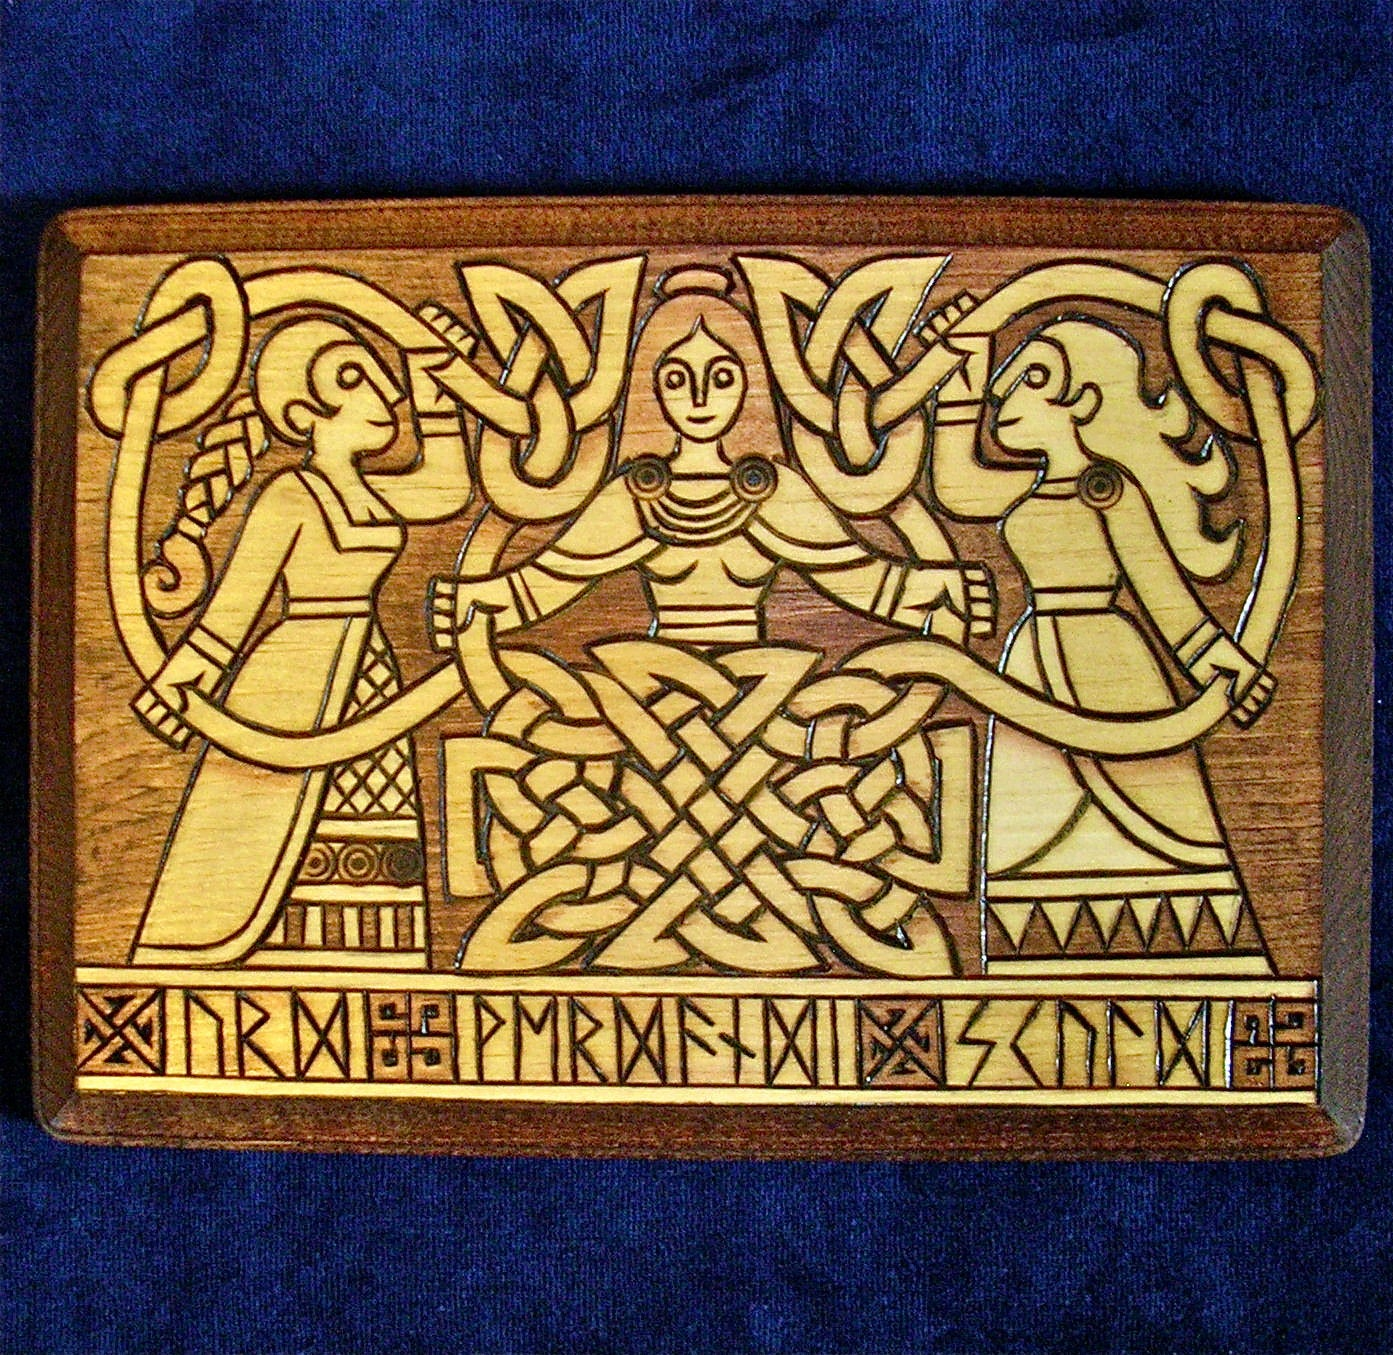
\includegraphics[trim={0 0 0 3cm},clip, width=1.5\textwidth]{figures/Others/il_fullxfull.354517109_sgyq.jpg}} % Override the page setting and occupy it all.

            % Fill the rest of the page
            \vfill  
            
        %\end{flushleft}
        \end{left}
    }  % There is an error here which complain that \begin{left} is math mode and is not closed with $$. It works fine, ignore it.
\end{center}
\cleardoublepage


%--------------------------------------------------------------------------------
% Preamble
%
% This part is just for enumerating the first chapters with Roman numbers.

% This includes:
% (i)   Preface,
% (iii) Acknowledgements
% (v)   List of papers
% (vi)  List of abbreviations
% (x)   English abstract
% (xi)  Norwegian abstract
%--------------------------------------------------------------------------------
\pagenumbering{roman} 				% Begin Roman page numbering (i,ii,...)




%---------------------------------------------------------------------------
% Preface
%---------------------------------------------------------------------------
\chapter*{Preface}
    \addcontentsline{toc}{chapter}{Preface}

        Social influence has been a notion nesting in human brains since we started living in a community. In the Poetic Edda, the poems of Fáfnismál \cite{ref:SagaBook}\cite{ref:Saga1} and Völuspá \cite{ref:Saga2} describe the existence of beings known as the “Nornir”, who are in charge of weaving the threads of destiny for gods and humans alike. Völuspá describes the Nornir as three individuals: Urðr (“Fate”), Verðandi (“What Is To Come”), and Skuld (“What Needs To Occur”). In Germanic folklore, fate is not fixed nor unique. Because of the influence of others, and because of our own past actions, humans do not have complete freedom to do what they want, but we are not enslaved by divine determinism either. The Nornir are constantly knitting the tapestry of life, in which each person's string is tugging with those of others, always changing and defining who we are or will be.

        A thousand years later, Jean Jacques Rousseau argues that we surrender our freedom to the "community". Rousseau synthesized the transition from natural freedom to civil liberty with the phrase: \textit{“Freedom consists not so much in doing one’s will as in not being subjected to that of others; it still consists in not submitting the will of others to ours“} \cite{ref:RousseauBook}. Rousseau argued that one must surrender his freedom and act in the best interest of the "general will" because by definition the general will can never be wrong. This "general will" has been used as justification for preserving liberty and to build the foundations for 20th-century totalitarianism enforcing oppression. In contrast, John Locke argued that there are rights undeniable to each individual, and no government, not even the general will, has the right to take them away.

        This begs the question, if other people always influence us and we are vulnerable to others' ideas, is freedom an illusion? In my thesis, I argue that your health is not different and will never be alone. Your social network has been estimated to weigh between 15\% to 40\% \cite{ref:socialinfluence2014} of the relative contributions from health determinants (such as genetics, environment, or medical care) to health outcomes. You are forced to be part of a community and you need to understand the trade-off of your options. People give you the risk of being infected by pathogens, but isolation makes you more likely to have alcohol addiction or suffer from depression. Friends will influence you to skip diets and drinks at the bar, advertisers will constantly push you to consume junk food. Do you eat what you want or do you eat what is enforced upon you? Do you choose your health or is it imposed by others?

        You are locked in the tapestry with other people and they are always influencing your fate, but you are still in charge of it. Being part of a group doesn't excuse you from being responsible for your actions. Being aware of that influence allows you to act with freedom and not necessarily by obeying the will of others. I invite you to read this work and how we measure such influences and their consequences, how to recognize them, and how to avoid them, in the hope that you use this knowledge to preserve the elemental health rights of individuals.

        This thesis is the product of my work at the Department of Computer Science, UiT The Arctic University of Norway, Tromsø, to obtain the Philosophiae Doctor of Science.

        Rafael Adolfo Nozal Cañadas
        \today

    \cleardoublepage


%---------------------------------------------------------------------------
% ENGLISH ABSTRACT (250-ish Words)
%---------------------------------------------------------------------------
\chapter*{Abstract}
\addcontentsline{toc}{chapter}{Abstract}

\textbf{Research questions:} The primary objective of this doctoral dissertation is an explorative investigation into the social network dynamics within eight high schools, located in Tromsø and Balsfjord (North Norway), and the extent to which these dynamics contribute to the overall health and well-being of the students, such as in the context of infectious disease spread and the transmission of negative or positive health effects, and also in comparison with non-social host factors such as sports or recreational drug frequencies. Secondarily, we aim to develop new analytical methods and provide a framework for enabling agnostic evaluation of social networks in epidemiological studies and faster iterations of developing scripts for general statistical research.

\vspace{0.70\baselineskip} % Increase paragraph spacing manually so this section doesn't end in a weird cut-off paragraph on the second page

\textbf{Methodology:} Using the Fit Futures gathered data on friendship, we used simulations, homophily, $X^2$ tables, logistic regression, and random forests as the main methods to analyze social influence in our topics of interest. We applied classical database normalization and data cleaning to the original data and developed scripts for automatic analysis in R and Python exporting results directly in plain text, Latex, and HTML.

\vspace{0.70\baselineskip}

\textbf{Results:} We found that the social network influences significantly the spread of \gls{staph}. Students close in the network tend to have similar inflammatory biomarkers, \gls{25ohd}, and \gls{bmi} levels. Some high schools tend to consume similar levels of over-the-counter medicines and tend to share the same brand of prescribed medicines. There is also a bias on recreational drug usage by high school.

\vspace{0.70\baselineskip}

\textbf{Conclusions:} Social influence is shown to be significant in every analysis. These findings emphasize the importance of considering social network dynamics in understanding and addressing health and well-being issues among students. Further research and interventions targeting social network influences can contribute to developing more effective health strategies.


\vspace{0.70\baselineskip}

\textbf{Originality:} Use of non-parametric simulation and machine learning methods to estimate social influence. We are measuring social influence on \gls{25ohd}, in an inflammatory proteomic assay.

\vspace{0.70\baselineskip}

\textbf{Significance:} Social influence, whether from virtual friends or physical ones, is a growing area of interest in many fields. In Epidemiology in particular we saw a boost in popularity after the Sars-Cov-2 pandemic.

\vspace{0.70\baselineskip}

\textbf{Keywords:} Social Networks, \gls{staph}, statistics, epidemiology, vitamin D, obesity, inflammation, random forests, prescriptions, drugs.


    
%---------------------------------------------------------------------------
% Acknowledgements
%---------------------------------------------------------------------------
\chapter*{Acknowledgements}
\addcontentsline{toc}{chapter}{Acknowledgements}

    A fair listing of all the positive qualities and contributions of everyone connected to this thesis would render another 200 pages, and would still be the short version of it. Instead, I hope that the people named here would forgive me for describing only one or two of the many good characteristics that helped in this PhD journey.

    First, I want to express my gratitude to \gls{bin} and the UiT The Arctic University of Norway for providing financial support, and \gls{rek} and the Norwegian Data Protection Authority for approval of the data collection (reference: 2018/1975/REK Nord).
 
    I would like to express my sincere gratitude to my main supervisor Lars-Ailo Bongo for his invaluable contributions to this project. His writing feedback has been incredibly thorough and detailed, providing me with the guidance and support I needed to refine my work and take it to the next level. In addition, his high level of expertise and knowledge in many fields has been instrumental in shaping the direction and scope of this project. His insights and recommendations have been invaluable, and I feel fortunate to have had the opportunity to work with someone of such exceptional talent and dedication.

    Co-supervisors Anne-Sofie Furberg and Anne Merethe Hanssen have provided valuable insights and expertise in the areas of general medicine and microbiology, which have helped to shape this project, and been a source of moral support throughout this project, providing encouragement and motivation. They have also introduced me to other individuals, listed below, who have later made significant contributions to this project.

    Christopher Nilsen for his invaluable contributions to this doctoral thesis. Christopher played a pivotal role in the conceptualization of Fit Futures. In particular, he also insisted on the inclusion of the social network data that made this PhD research possible. His foresight was critical in shaping the direction of this research and many others as he is persistently securing funding for new projects.

    To my department leader Anders Andersen and his efforts to improve the department's resources thanks to which I had the means to do this PhD.

    Other co-authors in this project are Dina Benedicte Berg Stensen, Mohsen Askar. I would like to express my deep appreciation to them for their invaluable contributions to the scientific articles we have worked on together. Their expertise in the fields of endocrinology and pharmacy has been essential in shaping the direction and scope of our research, and their collaboration has been instrumental in bringing these papers to fruition. Their dedication, hard work, and attention to detail have been truly inspiring, and I feel grateful to have had the opportunity to work with such talented and knowledgeable individuals.
    
    Other co-authors in other projects, Rocío Raya Miranda and María Luz Gamiz Perez. I did my first statistical course ever with Rocío and I will be forever grateful for her introducing me to this world. María Luz continued teaching me biostatistics and survival analysis later on in my studies. Hopefully, I have become a productive member of this community and thanks to them I have grown to the point that I could teach them a thing or two and we share co-authorship in several articles.

    Other collaborators Rocío Bonillo León, Svendsen Kristian, Lars Småbrekke, Guri Grimmes. I don't have a background in medicine, but thanks to them I gained a deeper understanding of many topics, including nutrition, pharmacology, immunology, endocrinology, and physiology. For me is important to get the best mental image possible of how things work rather than crunching the numbers and hoping that someone else deals with the results.

    All other group coworkers for their continuous feedback, encouragement, and dedication to showing me and others how to push the boundaries of knowledge. Also, to the cleaning crew in the UiT, for their tireless efforts, their hard work and dedication often go unnoticed, but their contributions are invaluable to the smooth operation of the university. Without their daily efforts, the university would not be able to function effectively. And finally to the personnel in charge of making food in the cafeteria. Their commitment to providing nutritious and delicious meals to the university community is greatly appreciated and kept me running many endless days in the office.

    All their valuable wisdom and efforts encourage me and others to reach our full potential.

\cleardoublepage


%---------------------------------------------------------------------------
% LIST OF PAPERS
%---------------------------------------------------------------------------
\chapter*{List of papers}
\label{chapter:chapterListPapers}
\addcontentsline{toc}{chapter}{List of papers}

    This thesis is based on the following papers, available in the appendix section \ref{chapter:annexPapers}.
    
   \begin{description}

        \item[\colorbox{PaperColor}{\textcolor{black}{Paper A:}}]{ Stensen DB, Cañadas RAN, Småbrekke L, Olsen K, Nielsen CS, Svendsen K, Hanssen AM, Sollid JUE, Simonsen GS, Bongo LA, Furberg AS. Social network analysis of Staphylococcus aureus carriage in a general youth population. International Journal of Infectious Diseases Volume 123, October 2022, Pages 200-209 \url{https://doi.org/10.1016/j.ijid.2022.08.018}}

        \item[\colorbox{PaperColor}{\textcolor{black}{Paper B:}}]{ The Social Sunshine of the Arctic Youth: Exploring friendship's influence on Vitamin D levels. Cañadas RAN, Nielsen CS, Furberg AS, Hanssen AM, Bongo LA \url{https://www.medrxiv.org/content/10.1101/2023.11.29.23299188v1.full.pdf}}
        
        \item[\colorbox{PaperColor}{\textcolor{black}{Paper C:}}] { Askar M, Cañadas RAN, Svendsen K. An introduction to network analysis for studies of medication use. Research in Social and Administrative Pharmacy Volume 17, Issue 12, December 2021, Pages 2054-2061 \url{https://doi.org/10.1016/j.sapharm.2021.06.021}}        

    \end{description}

    In addition, the following results are a summary of another four manuscripts that have not yet been published, which can be found in the appendix section \ref{chapter:chapter results}. 

    \begin{description}

        \item[\colorbox{ResultColor}{\textcolor{black}{Result I:}}]{Social network influences on obesity in a general youth population}

        \item[\colorbox{ResultColor}{\textcolor{black}{Result II:}}]{Social network influences on inflammatory response in a general youth population}

        \item[\colorbox{ResultColor}{\textcolor{black}{Result III:}}]{Measuring social influence with random forest regression and artificial neural networks.}

        \item[\colorbox{ResultColor}{\textcolor{black}{Result IV:}}]{Frequency consumption of medication and social network influence in a general youth population.}
        
    \end{description}

%---------------------------------------------------------------------------
% LIST OF ABBREVIATIONS
%
% These are displayed in alphabetical order
%---------------------------------------------------------------------------
%\chapter*{List of abbreviations}
\addcontentsline{toc}{chapter}{List of abbreviations}

\glsnogroupskiptrue  % Don't skip the line between abbreviations group
\printglossary[type=\acronymtype,title=Abbreviations]





%---------------------------------------------------------------------------
% TABLE OF CONTENT
%
% This is generated automatically, you don't need to write anything
%---------------------------------------------------------------------------
\setcounter{tocdepth}{1}            % Sets the number of section levels in the table of contents to 1
                                    % 0 = Chapters only
                                    % 1 = Sections only
                                    % 2 = Sub-sections only
                                    
\tableofcontents                    % Creates the table of contents

\glsunsetall                        % Avoid symbols to be triggered in the list of figures / tables but rather in the body of the text later


\cleardoublepage
% \phantom section so the "List of Figures" appears in the list of contents
\addcontentsline{toc}{chapter}{\listfigurename}
\listoffigures


\cleardoublepage
% \phantom section so the "List of Tables" appears in the list of contents
\addcontentsline{toc}{chapter}{List of Tables}
\listoftables

\glsresetall

\cleardoublepage                    % Ends the current page


%---------------------------------------------------------------------------
% Chapters
%---------------------------------------------------------------------------
\pagestyle{fancy}               	% Fancy headings
\pagenumbering{arabic}				% Begin arabic page numbering (1,2,...)
\setlength{\parindent}{20pt}        % Sets default paragraph indentation to 20 pt 

% Introduction to networks
%*****************************************
\chapter{Introduction}
\label{chapter:chapter intro}
%*****************************************

\section{ Social Network Analysis in health }

In recent years there has been a growing recognition of the profound impact that social relationships and networks of friends have on health outcomes (figure \ref{figure:networkNetworkRise}). This includes common and well-known topics such as the spread of obesity \cite{Christakis2007, Trogdon2008}, recreational drugs usage such as smoking \cite{Christakis2008, Aschbrenner2018} alcohol \cite{Rosenquist2010, Ali2014} or cannabis \cite{Mednick2010}, and  depression \cite{Rosenquist2010}.

    \begin{figure}[H]
        \centering
            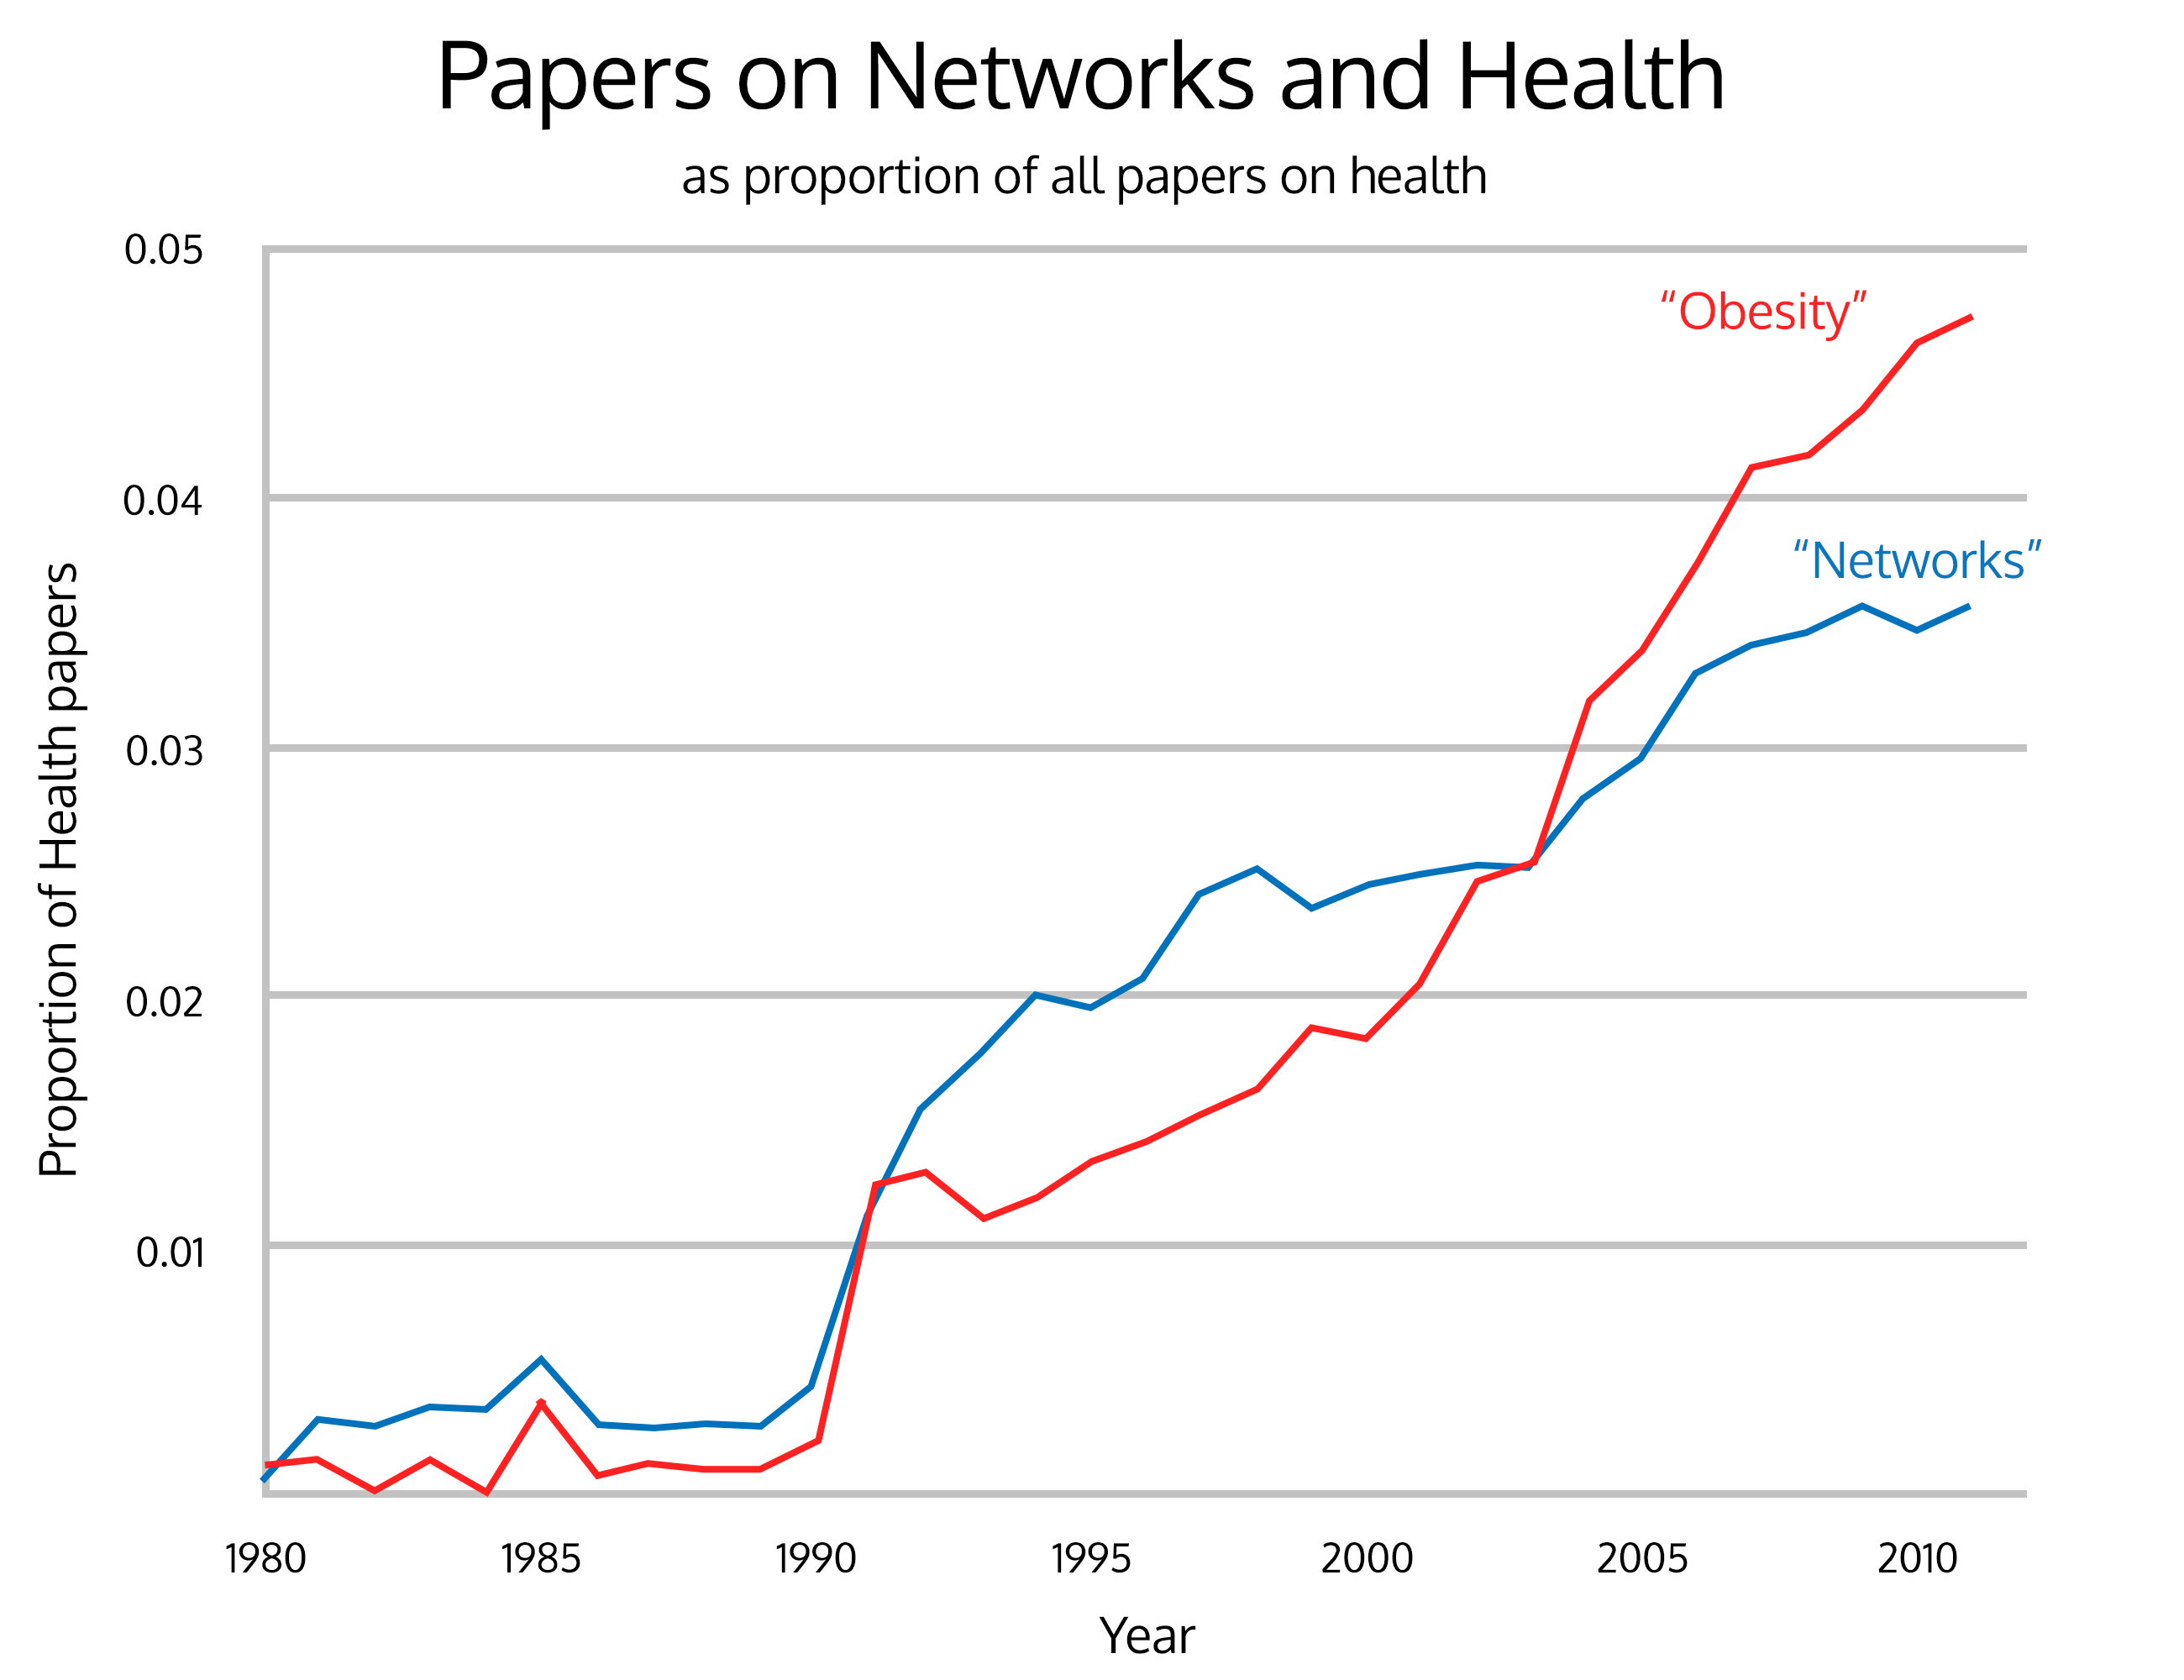
\includegraphics[width=0.7\linewidth]{figures/Social/paperSocialRemastered.png} 
        \caption{Proportion of papers published about networks on the topic of health across the years, compared with the number of papers published on obesity. Image reproduced with permissions from "International Encyclopedia of the Social and Behavioral Sciences" \cite{ref:networkRises}.}
        \label{figure:networkNetworkRise}
    \end{figure}

\gls{sna} is a powerful tool for understanding how social connections influence health behaviors, disease transmission, and healthcare access. This thesis leverages \gls{sna} techniques to explore the dynamic interplay between social networks and health, aiming to provide valuable insights that can inform interventions, policies, and practices for improving health outcomes.

\section{ Social network interventions }
\label{socialinterventions}

Within the realm of health research, \gls{sna} has demonstrated its versatility and applicability across a wide range of topics. It is possible to detect early outbreaks of influenza \cite{Christakis2010}. To prevent the spread of \gls{hiv} infections \cite{Friedman1997}. To improve the life of chronic illnesses patients as well as their families and community \cite{FernndezPea2020}. It has been shown that information on social networks can increase the prediction of health-related models at around 50\% \cite{Lin2019}. It has been used to design interventions and strategies to enhance communication, collaboration, and knowledge sharing among health professionals, ultimately improving the overall performance and effectiveness of the health organization \cite{Tasselli2014, Sabot2017}. A systematic review of 37 studies suggests that social network interventions are associated with positive health behaviors and outcomes \cite{Hunter2019}. And of course, social network interventions have been used to better the outcome of obesity \cite{Gesell2013, systems9030066, Smith2020, McGlashan2019}, mental health \cite{Pinto2005, Rosychuk2009}, overcoming tobacco addiction \cite{Latkin2015, Sadasivam2016},  transmittable diseases in humans \cite{Danon2012, Wang2011, Llupi2016, Ljubic2019} and in cattle such as cows, sheep, and pigs \cite{Marquetoux2016, OrtizPelaez2006}, and recently we experienced these interventions first hand with COVID-19 \cite{Corcoran2022, Centola2020}.

These few examples show that \gls{sna} has proven practical value in understanding the diffusion of diseases, as well as tracking the spread of infectious agents through clusters or interconnected social groups. It has been found to play a crucial role in improving individuals' health and preventing further deterioration of their well-being. Different authors have evaluated that social relationships influence a person's health between 15\% to 40\% \cite{ref:socialinfluence2014}, putting it ahead of the environment and even medical care. And yet it remains a vastly under-utilized and underrated technique.

\section{ Thesis impact }

In this thesis, we employ \gls{sna} techniques to shed light on the complex relationships between social networks and health outcomes within a specific population. We have shown how \gls{staph}, vitamin D, inflammation, medication usage, and obesity are influenced by social networks in a general youth population in Tromsø. We also expanded non-parametric methods for group comparisons in graphs using simulations and applied machine learning models to measure the influence of peers on obesity. Finally, we lay down the basics for a framework to obtain a more efficient analysis framework. We hope this leads to a significant contribution to public interventions and policies that ultimately lead to improved health outcomes in Norway and beyond.


% Aims of the thesis
%*****************************************
\chapter{Aims of the thesis}\label{ch:aims}
%*****************************************

%\colorbox{PaperColor}{\textcolor{black}{Paper}}
%\colorbox{ResultColor}{\textcolor{black}{Result}}


% S - Who and What

The overarching objective of this research is to develop methodologies and conduct exploratory studies to  evaluate the impact of social influence on a range of health-related topics. This work targets several topics and is done with the help of an interdisciplinary team of health professional researchers. In parallel, this work aims to provide a framework that enables researchers to facilitate faster analysis and produce improved visualizations. 

% M - By how much

The results of these studies must be a quantifiable measure of how much measuring or modifying the social networks could benefit the studied population. Secondarily, speculate how these results could affect the general population and the advantages and disadvantages of influencing and changing their social network.

% A - How?

The first step of our research is to study how infections and the immune system behave in the population. First, by measuring the spread of \gls{staph} \colorbox{PaperColor}{\textcolor{black}{(Paper A)}} and investigating the possibility that inflammatory processes may be similar across individuals or schools \colorbox{ResultColor}{\textcolor{black}{(Result II)}}. The second step is to inspect the social aspect of obesity with classical methods \colorbox{ResultColor}{\textcolor{black}{(Result I)}} and using machine learning models \colorbox{ResultColor}{\textcolor{black}{(Result III)}}. Lastly, we look into other variables of interest such as how friends influence vitamin D levels \colorbox{PaperColor}{\textcolor{black}{(Paper B)}} or medication usage \colorbox{ResultColor}{\textcolor{black}{(Result IV)}}.

For our secondary objectives, we want to present tutorials and proof of concept on how to apply \gls{sna} techniques. For this, we choose prescriptions and drug interactions \colorbox{PaperColor}{\textcolor{black}{(Paper C)}}. We also want to present a user-friendly wrapper library to abstract away the complexity and details of \gls{sna} and other statistic and machine learning models, where biases are checked automatically, fundamental analysis reports are generated with minimal intervention from the programmer, and plots or figures follow basic design rules for good visualization.

% R - Why?

Starting with infectious diseases is a good starting point as it is the classical topic for understanding the network structure, and testing and developing new methods. It also has the advantage of updating targeted interventions in similar populations in the future. Later on, obesity in particular is a good topic for \gls{sna} due to having a substantial impact on individual lifestyle choices, including diet, exercise, and weight management; all of which are influenced by friends. Lastly, topics such as vitamin D levels are purely explorative and we want to determine if there was a connection with the social network.

Regarding our programming objective, wrapper libraries serve as a layer of abstraction that simplifies the usage of lower-level functionality, allowing programmers to build applications more efficiently and with less effort. We also want to extend these advantages and make a high-level abstraction in the statistical context.

%The first step of our research involved measuring the spread of \gls{staph} \colorbox{PaperColor}{\textcolor{black}{(Paper A)}} and investigating the possibility that inflammatory processes may be similar across individuals or schools \colorbox{ResultColor}{\textcolor{black}{(Result II)}}. With this initial groundwork laid, we did further analyses. We continued to explore other metrics, such as the influence of obesity \colorbox{ResultColor}{\textcolor{black}{(Result I)}} and vitamin D \colorbox{PaperColor}{\textcolor{black}{(Paper B)}} among other measures. 

%Additionally, we used machine learning models to measure social influence on obesity \colorbox{ResultColor}{\textcolor{black}{(Result III)}}. We also reported medicine usage in this population and how friends can influence this behavior \colorbox{ResultColor}{\textcolor{black}{(Result IV)}}. We also presented a tutorial and proof of concept on how to apply \gls{sna} in prescriptions and drug interactions \colorbox{PaperColor}{\textcolor{black}{(Paper C)}}.






%Throughout the process, I aimed to provide guidelines regarding the data cleaning process, we applied \gls{bcnf} to the data to save valuable time. 


% S - Who and What
% M - By how much
% A - How?
% R - Why?





\vspace{0.90\baselineskip}



% Introduction to Staph and others
\input{chapters/ChapterBACKGROUND}

% Materials and methods
%*****************************************
\chapter{Methodology}\label{ch:methodology}
%*****************************************

\section{Fit Futures}

The \gls{ff} study \cite{ffreference} is a cohort with repeated health surveys among high school students in the Norwegian municipality of Tromsø and the neighboring municipality of Balsfjord. This dataset is the main dataset used across all results of the thesis. All first-year high school students in Tromsø and Balsfjord were invited. FF1 was conducted from September 2010 to May 2011 for 8 months. FF1 included students from eight schools consecutively. A total of 1117 youths were invited 93\% attended, 508 girls (48.9\%), and 530 boys. The age ranges from 15 to 28 years old, with 822 (79.2\%) being 16 years old or younger, and 52 (5\%) older than 18 years old. Older students with special educational needs or mental disabilities have the right to study at the high school level in Norway. In figure \ref{figure:hsLocations} we can see the geographical distribution of the schools and in table \ref{table:SummarySchools} information specific to each school.

\gls{ff2} is a follow-up survey conducted from November 2012 to June 2013. FF2 invited all participants in FF1 and all new students from the third year at the eight high schools. Altogether 870 high school students were recruited in the FF2 study, and 78\% of these attended both surveys. In the papers comprising this thesis, we only used FF2 anthropometrical data. However, FF2 included the same variables present in FF1, but we did not have access to this data. In FF2, 694 students (66.9\% of the FF1 total) completed the anthropomorphic measurements, 378 girls (54.5\% of total participants), and 316 boys. Some students in the vocational training program did not get permission from work to attend the FF2 follow-up measures, which contributed to lowering the total student count in the follow-up study.


    \begin{figure}[ht]
        \centering
            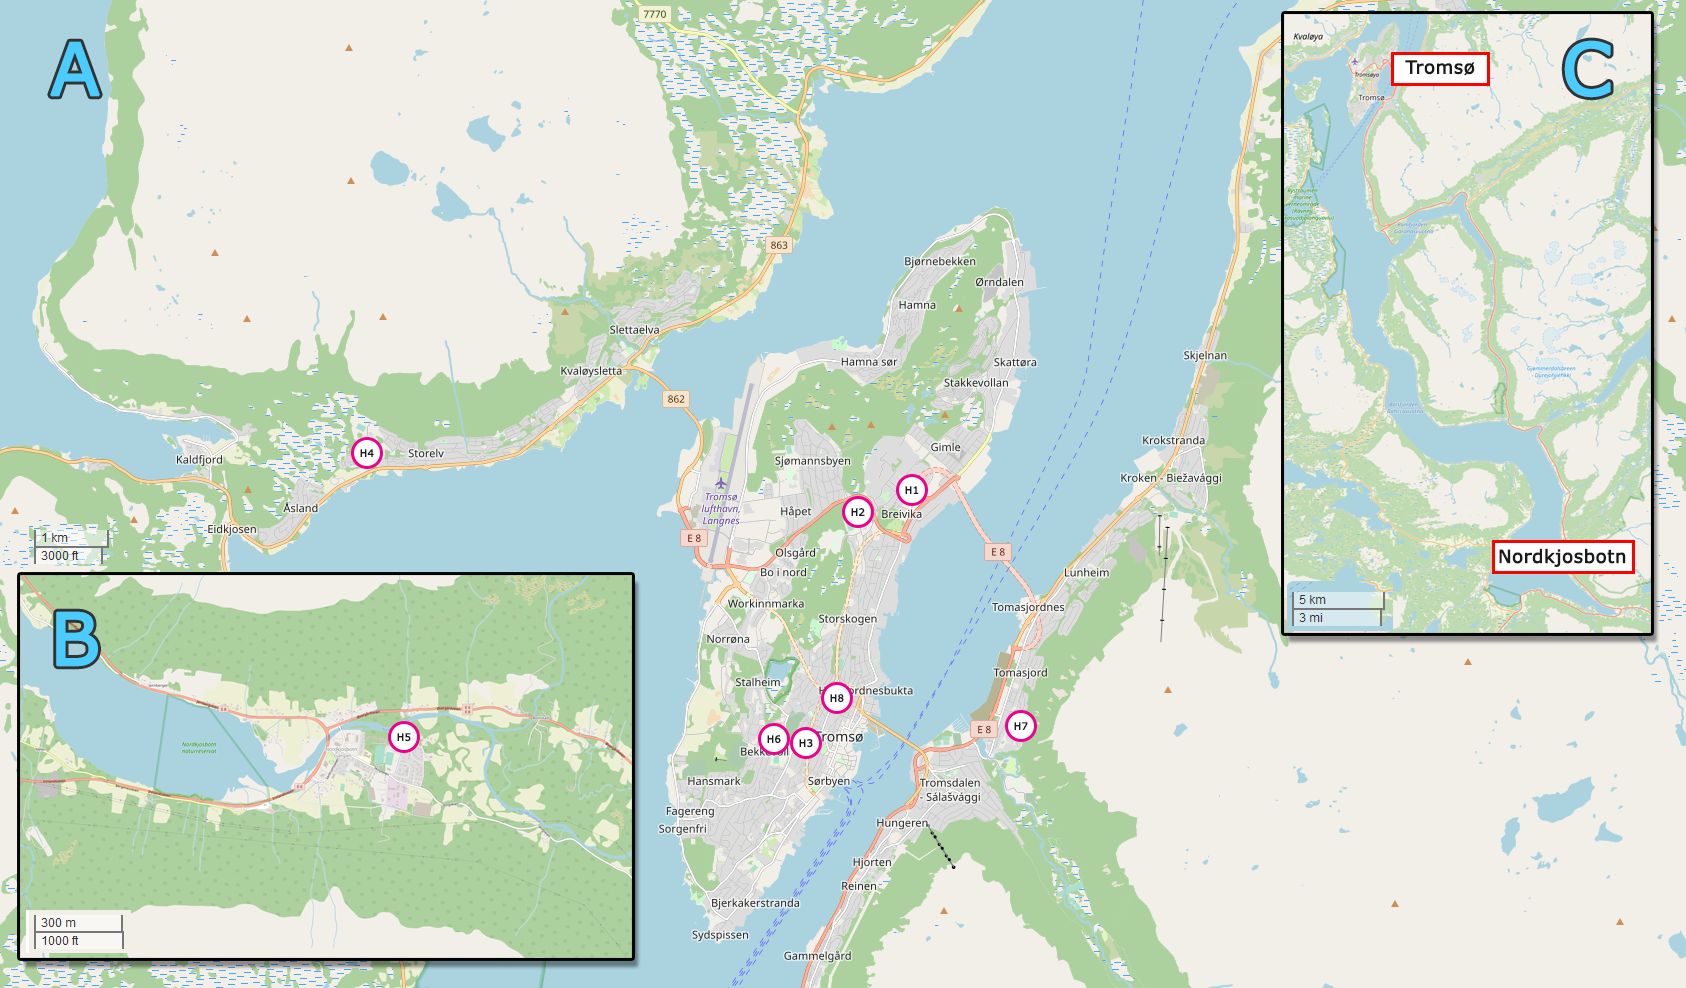
\includegraphics[width=0.9\linewidth]{figures/Methodology/schoolmaps.png } 
        \caption{Geographical location of all eight high schools included in the Fit Futures study. "A" refers to the area around Tromsøya, and "B" is the area in the town of Nordkjosbotn (Balsfjord). "C" shows the distance between "A" and "B".}
        \label{figure:hsLocations}
    \end{figure}

In FF1 and FF2, the participants had a one-day visit to The Clinical Research Unit at the \gls{unn}, which included clinical examinations, microbiological samples, blood samples, a web-based general questionnaire (chapter \ref{ch:Annex}), and an interview \cite{Winther2014}. All procedures were performed by trained research study nurses. 

FF11 and FF12 refer to short follow-ups performed during the FF1 period. In these sub-surveys, not all the data was gathered again; only a sub-sample such as the swabbing of the \textit{S. aureus}.

\subsection{Social network assessment}
\label{method:SocialNetwork}

The social network was constructed based on the following questions in the interview. These were written and answered in Norwegian, here we provide the English translation: \textit{“Which students have you had the most contact with the last week? Name up to 5 students at your own school or other schools in Tromsø and Balsfjord.”}. Reciprocity in the nomination was not mandatory. For each of the nominations, five “yes/no” questions assessed the type of contact they had with their nominations: \textit{“Do you have physical contact?”}, \textit{“Are you together at school?”}, \textit{“Are you together at sports?”}, \textit{“Are you together at home?”}, \textit{“Are you together at other places?”}. This resulted in five social networks: Physical Network, School Network, Sports Network, Home Network, and Other Network. Adding all the relationships together formed a sixth network that was called the Overall Network. Illustrations of all networks are presented in figure \ref{figure:allNetwork}.

Not 100\% of the students participated in the study, and some of the relationship information between them is lost (table \ref{table:SummaryLost}). The final analysis shows that some of the lost 134 IDs, were very popular, with up to 9 friends nominated.

    \begin{figure}[ht!]
        \centering
            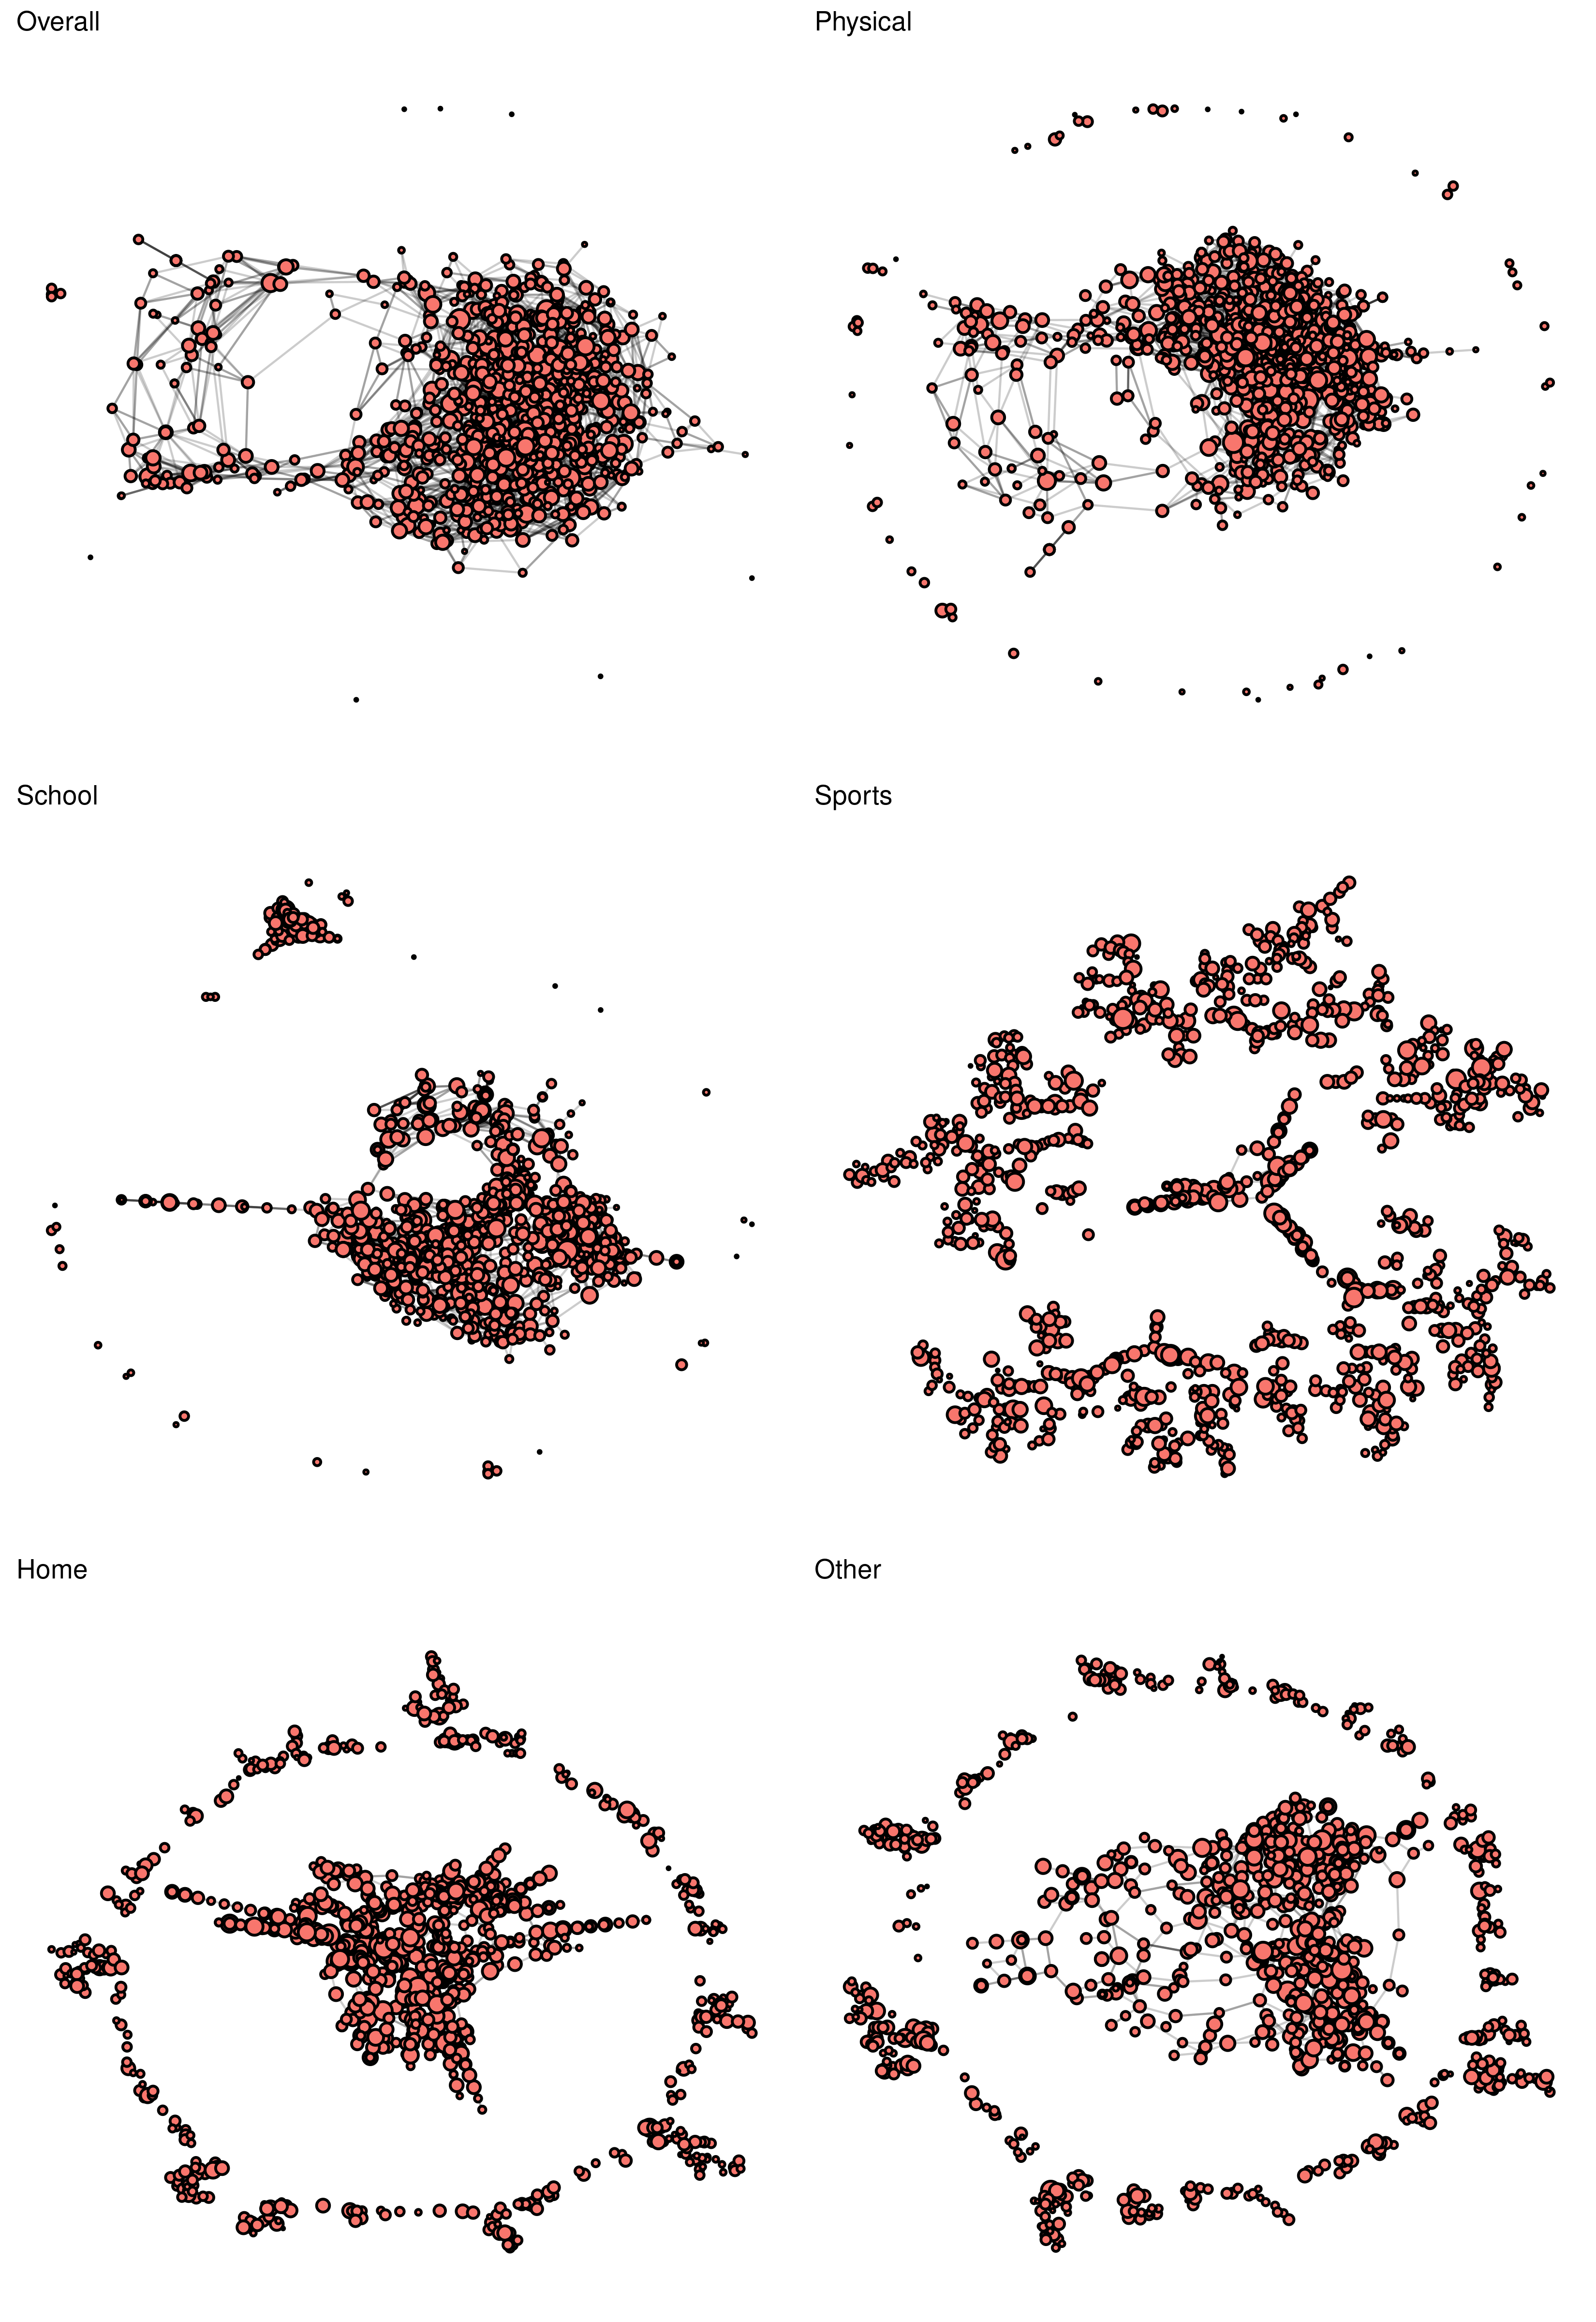
\includegraphics[width=0.8\linewidth]{figures/Methodology/allGraphs.png } 
        \caption{All networks in FF1 following a MDS layout. Each student is represented by one node in the network. Each relationship is represented by an undirected edge, i.e., a line, in the network.}
        \label{figure:allNetwork}
    \end{figure}

    
    \begin{table}[ht!]
    
        \caption{Information with the school names, study program, the total number of students in FF1, astronomical season, and whether a significant amount of students' blood samples were taken during the polar night.}

        \centering

        \label{table:SummarySchools}

        \scalebox{0.75}{
        
        \begin{tabular}{|
        >{\columncolor[HTML]{FFD5D3}}l |lllll|}
        \hline
        \cellcolor[HTML]{FFCCCC}ID           & \cellcolor[HTML]{FFFFC7}Name         & \cellcolor[HTML]{FFFFC7} Studies program &
        \cellcolor[HTML]{FFFFC7}FF1 Students & \cellcolor[HTML]{FFFFC7} Extraction & \cellcolor[HTML]{FFFFC7} Polar night \\ \hline
        
        H1   & Breivika videregående skole     & Vocational             & 207   & Autumn    & No   \\
        H2   & Breivang videregående skole     & Vocational and General & 142   & Autumn    & Yes  \\
        H3   & Kongsbakken videregående skole  & Vocational and General & 168   & Winter    & No   \\
        H4   & Kvaløya videregående skole      & Vocational and General & 98    & Spring    & No   \\
        H5   & Nordkjosbotn videregående skole & Vocational and General & 85    & Spring    & No   \\
        H6   & Norges Toppidrettsgymnas Tromsø & Sports                 & 26    & Spring    & No   \\
        H7   & Tromsdalen videregående skole   & Sports and General     & 192   & Winter    & Yes  \\
        H8   & Tromsø maritime skole           & Vocational             & 120   & Winter    & Yes  \\ \hline
        
        \end{tabular}

        }
    
    \end{table}

To evaluate if the friends mentioned were representative of the participant's social network, the following question was asked: \textit{“To what degree does this table of friends give an overview of your social network? Please indicate on a scale from 0 (small degree) to 10 (high degree).”} Nominated friends that did not participate in FF1 were excluded from the analysis (n=134). In figure \ref{figure:networksRepresentative} we can see a histogram with all the answers.

    \begin{figure}[ht]
        \centering
            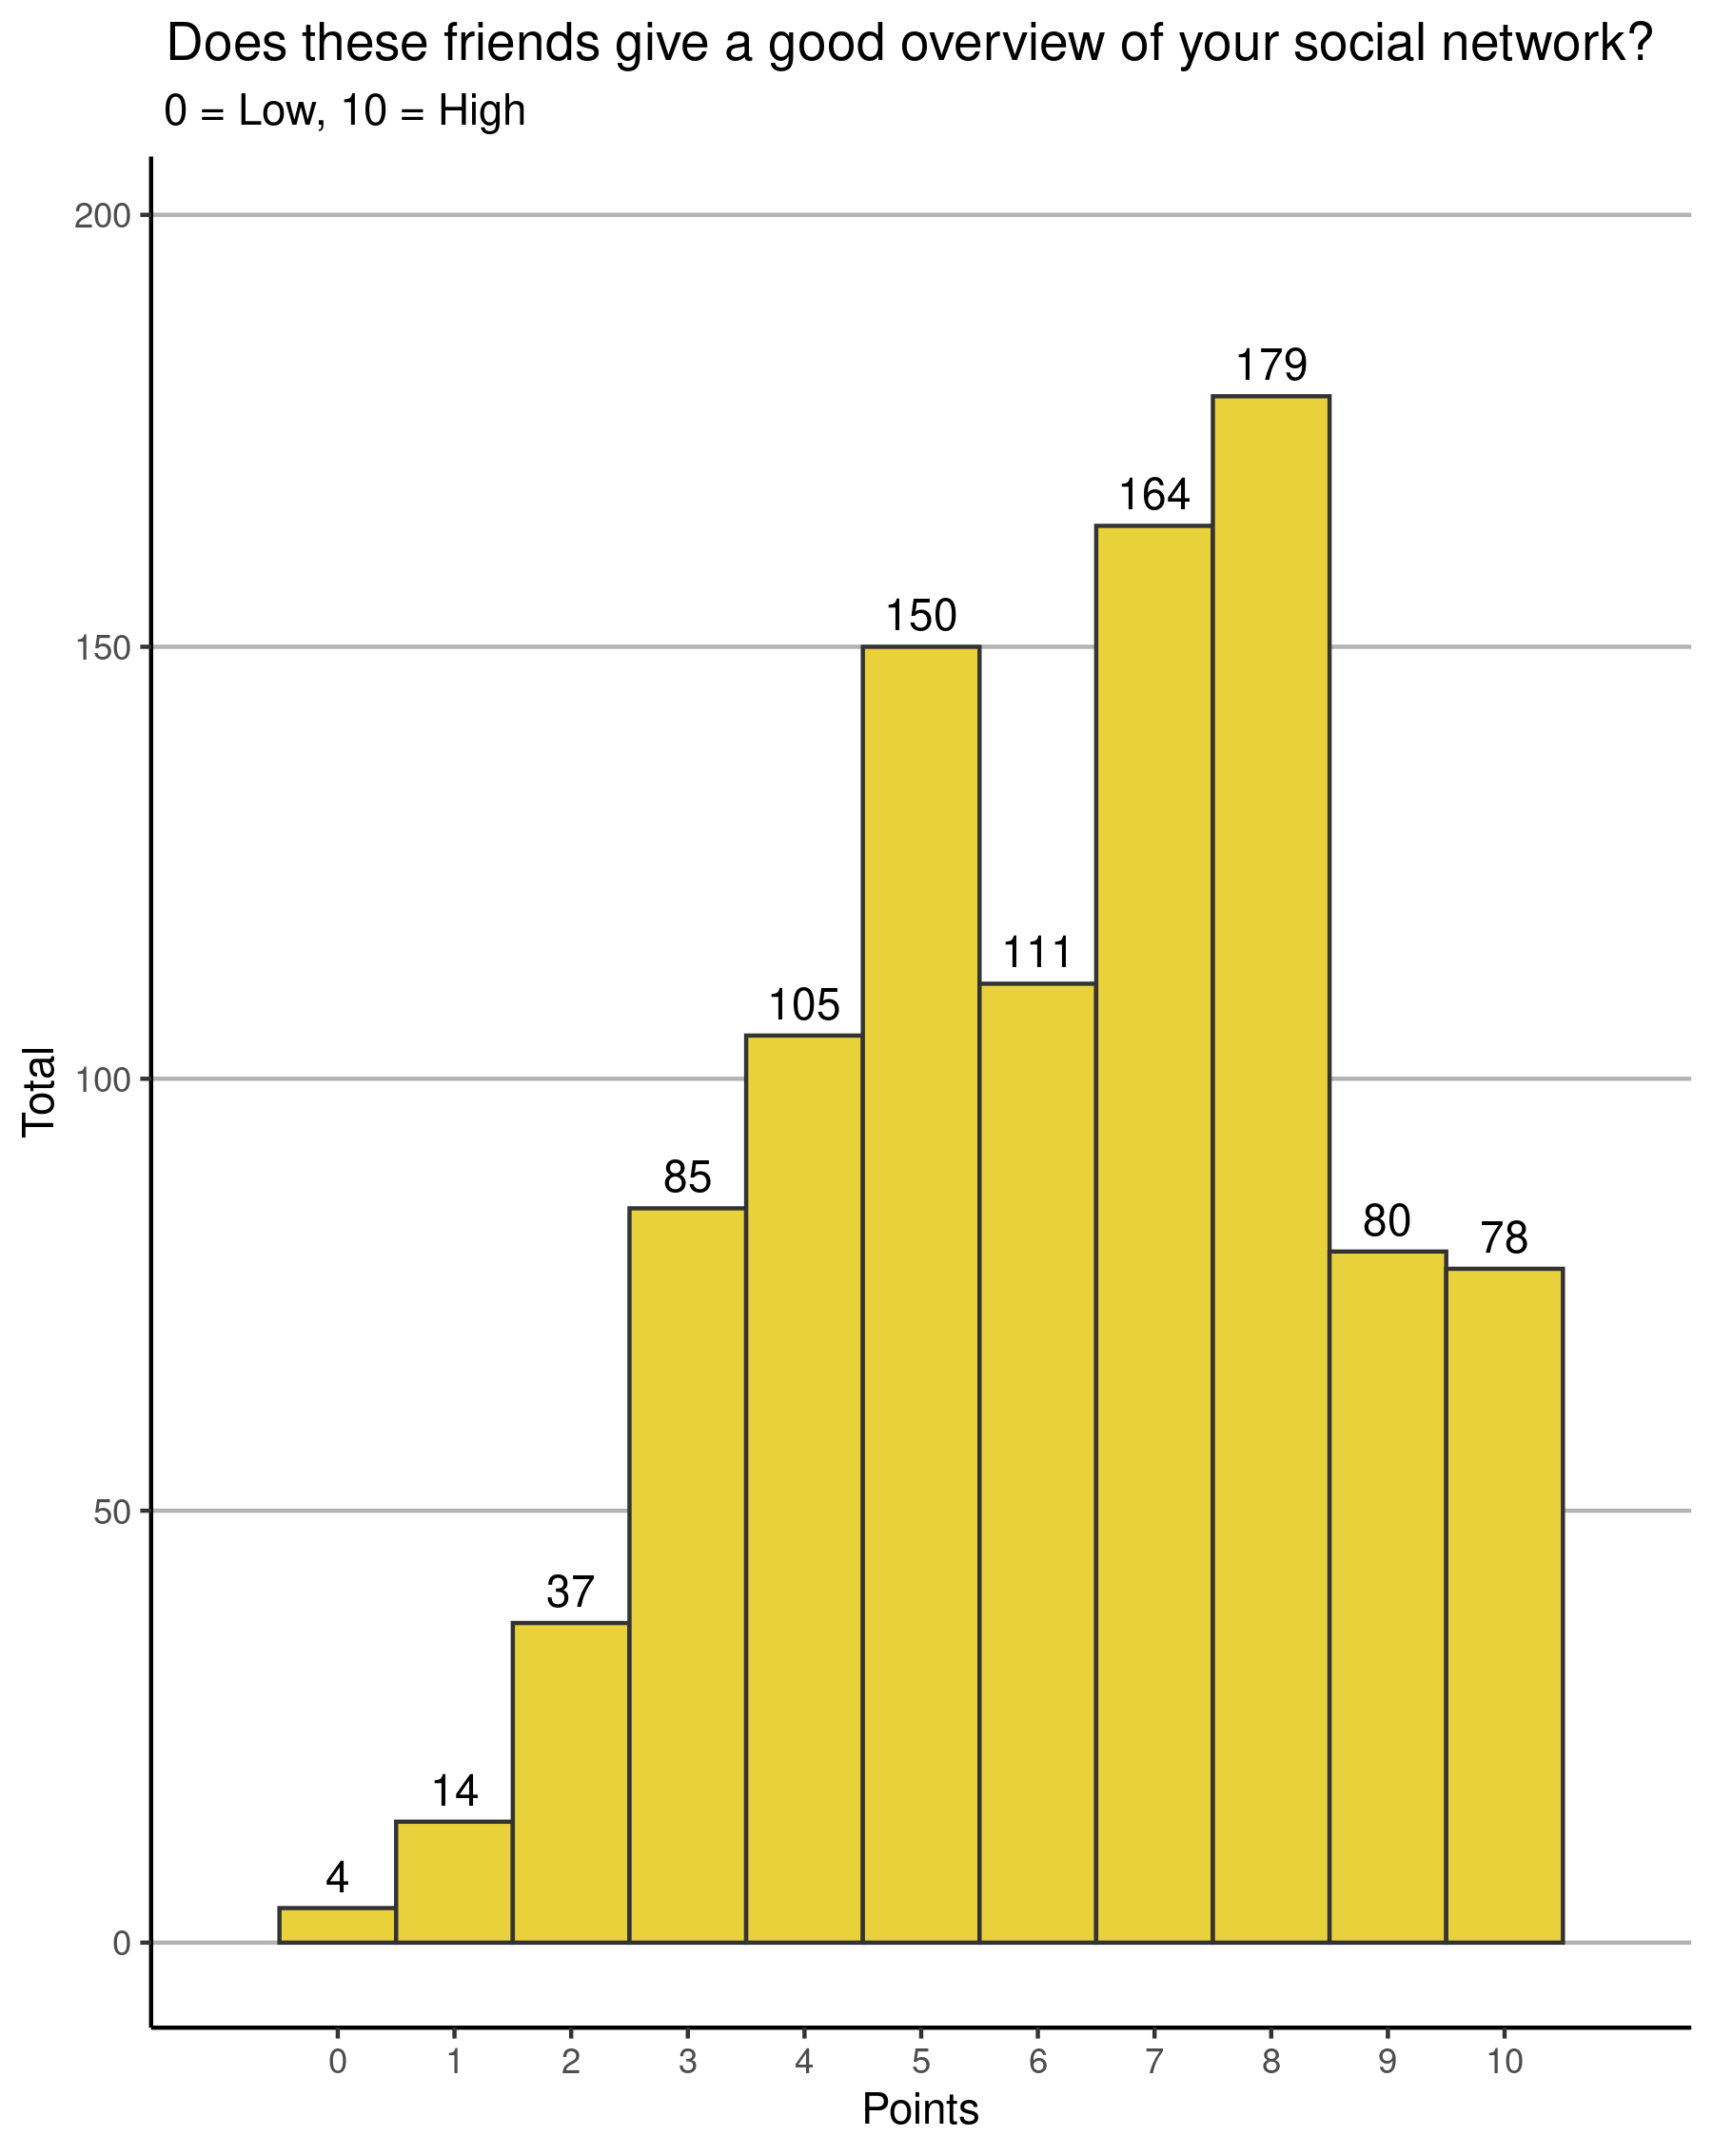
\includegraphics[width=0.55\linewidth]{figures/Methodology/Histogram_completeTable_Overview.png} 
        \caption{Histogram with all the answers to the question: \textit{“To what degree does this table of friends give an overview of your social network? Please indicate on a scale from 0 (small degree) to 10 (high degree).”}}
        \label{figure:networksRepresentative}
    \end{figure}



\begin{table}[ht!]

    \caption{Summary of lost connections at data cleaning.}

    \centering

    \label{table:SummaryLost}

 	\renewcommand{\arraystretch}{1.5} 

    \scalebox{0.75}{
  
    \begin{tabular}{ lll }
        \hline
        \rowcolor[HTML]{FFFFC7}

         \textbf{ Concept } &         \textbf{ Total } &         \textbf{ Relative } \\ 
        \hline 

        \multicolumn{1}{l|}{ Total IDs: } & 1177   & 100 \%          \\ 
        \multicolumn{1}{l|}{ - Total Deleted IDs: } & 139   & 11.81 \%          \\ 
        \multicolumn{1}{l|}{ - Total Remaining IDs: } & 1038   & 88.19 \%          \\ 
        \multicolumn{1}{l|}{ Total Edges: } & 4125   & 100 \%          \\ 
        \multicolumn{1}{l|}{  - Total Deleted Edges: } & 473   & 11.47 \%          \\ 
        \multicolumn{1}{l|}{  - Total Remaining Edges: } & 3652   & 88.53 \%          \\ 

    \end{tabular}
    
    }

\end{table}

\subsection{Host risk factors}

All questions related to sex, use of recreational drugs, dietary habits, chronic diseases, medication usage, sport frequency, sedentism, and so on, are self-reported using a web-based questionnaire.

\subsection{Hormonal contraceptive}

Information on current hormonal contraceptive use was obtained from the interview. \gls{hc} were categorized into combination contraceptives and progestin-only contraceptives. The combination contraceptives were further divided into groups according to high and low ethinylestradiol daily dosage. High dosage was defined as HC containing $\geq$ 30 μg ethinylestradiol. Low dosage was defined as contraceptives containing $\leq$ 30 μg ethinylestradiol. The classification for each brand can be seen in table \ref{table:hormonalDefinitions}.

\begin{table}[ht!]

    \caption{Types of hormonal contraceptives classification and their respective brands.}	

    \centering

    \label{table:hormonalDefinitions}

	\small

	\centering

    \scalebox{0.75}{

	\begin{tabular}{l|l}
	\hline
	\rowcolor[HTML]{FFAAAA} 
	Hormonal type                    & Contraceptive brand  \\ \hline
	Non-hormonal                     & Condoms              \\ \hline
    	                             & Cerazette            \\
        	                         & Nexplanon            \\
            	                     & Depo-provera         \\
	\multirow{-4}{*}{Progestin only} & Implanon             \\ \hline
    	                             & Mercilon             \\
        	                         & Yasminelle           \\
            	                     & Loette 28            \\
	\multirow{-4}{*}{Low Estradiol}  & Nuvaring             \\ \hline
    	                             & Marvelon             \\
        	                         & Yasmin               \\
            	                     & Microgynon           \\
                	                 & Oralcon              \\
                    	             & Diane                \\
                        	         & Synfase              \\
                            	     & Evra                 \\
	\multirow{-8}{*}{High Estradiol} & Zyrona               \\ \hline
	Unknown                           & Any other brand/type
	\end{tabular}
	
    }
	
\end{table}

\clearpage

\subsection{ \textit{S. aureus} assessment}

A first set of nasal and throat swab samples was taken at the research center, and a second set of samples was taken at school after a mean interval of 17 days. All 1038 students were sampled on both occasions, the first batch contained 1028 valid samples, and the second batch 988. A NaCl (0.9\%)-moistened sterile rayon-tipped swab rotated three times with gentle pressure was used to sample both vestibule nasi (nose sample), and an additional swab was used to sample both tonsillar regions (throat sample). The swabs were immediately placed in a transport medium (Amies Copan, Brescia, Italy) and stored at 4°C for a maximum of 3 days. All samples were analyzed at the Department of Microbiology and Infection Control, UNN, both by direct culture \cite{Olsen2011} and enrichment broth (Bacto Staphylococcus medium broth,(Difco Laboratories, Sparks, MD, USA - \cite{Stensen2019}), using blood agar for growth control (Oxoid, UK) and chromID-plates (SAID) for \textit{S. aureus} detection (bioMérieux, Marcy I’Etoile, France). A summary of these methods can be found in the supplementary materials. The growth of any bacterial colonies on agar plates was registered as a valid culture. The most dominating \textit{S. aureus} colony type was frozen at -70°C in glycerol-containing liquid media after confirmation by Staphaurex plus agglutination test (bioMérieux, Marcy I’Etoile, France).



From these results, \textit{S. aureus} nasal or throat persistent carriage was defined as having two \textit{S. aureus} positive cultures for each niche respectively. \cite{Nouwen2004, vanBelkum2009} Two definitions of \textit{S. aureus} persistent carriage was used in the analysis; one based on direct culture, and one based on enrichment broth. All results for every possible combination between the first or second sample, nasal or throat, direct culture or enrichment broth, and so on, can be found in figure \ref{fig:Carrier_definition}. 

%In our context, if a person has \textit{S. aureus} in one sample, we say this person is colonized by the bacteria. If the person has S. aureus in both samples, we say that the person is a persistent carrier. This applies to both the nose and the throat and both the direct culture and enrichment broth. In figure \ref{fig:Carrier_definition} we  encompass all the labeling workflow.

\subsection{SPA typing}

SPA-typing is a technique used to identify the \textit{S. aureus} strain. The gene encoding Spa is highly variable among strains of \textit{S. aureus}, making it a good target for distinguishing different types of bacteria \cite{Hallin2009}. The technique involves targeting the \gls{spa} located in the cell wall are described in the supplementary materials.

For the analysis of \textit{S. aureus} genotype, only data from throat isolates were available (n = 746). All \textit{S. aureus} isolates from throat samples were subjected to spa-typing. The frozen cultures were inoculated on blood agar (Oxoid) and incubated overnight at 37°C. Two or three colonies were transferred to 200 µl sterile\ch{H2O} and vortexed. The isolates were later spa-typed \cite{Sangvik2011}.

\clearpage

            \begin{figure}[!ht]
                \centering
                    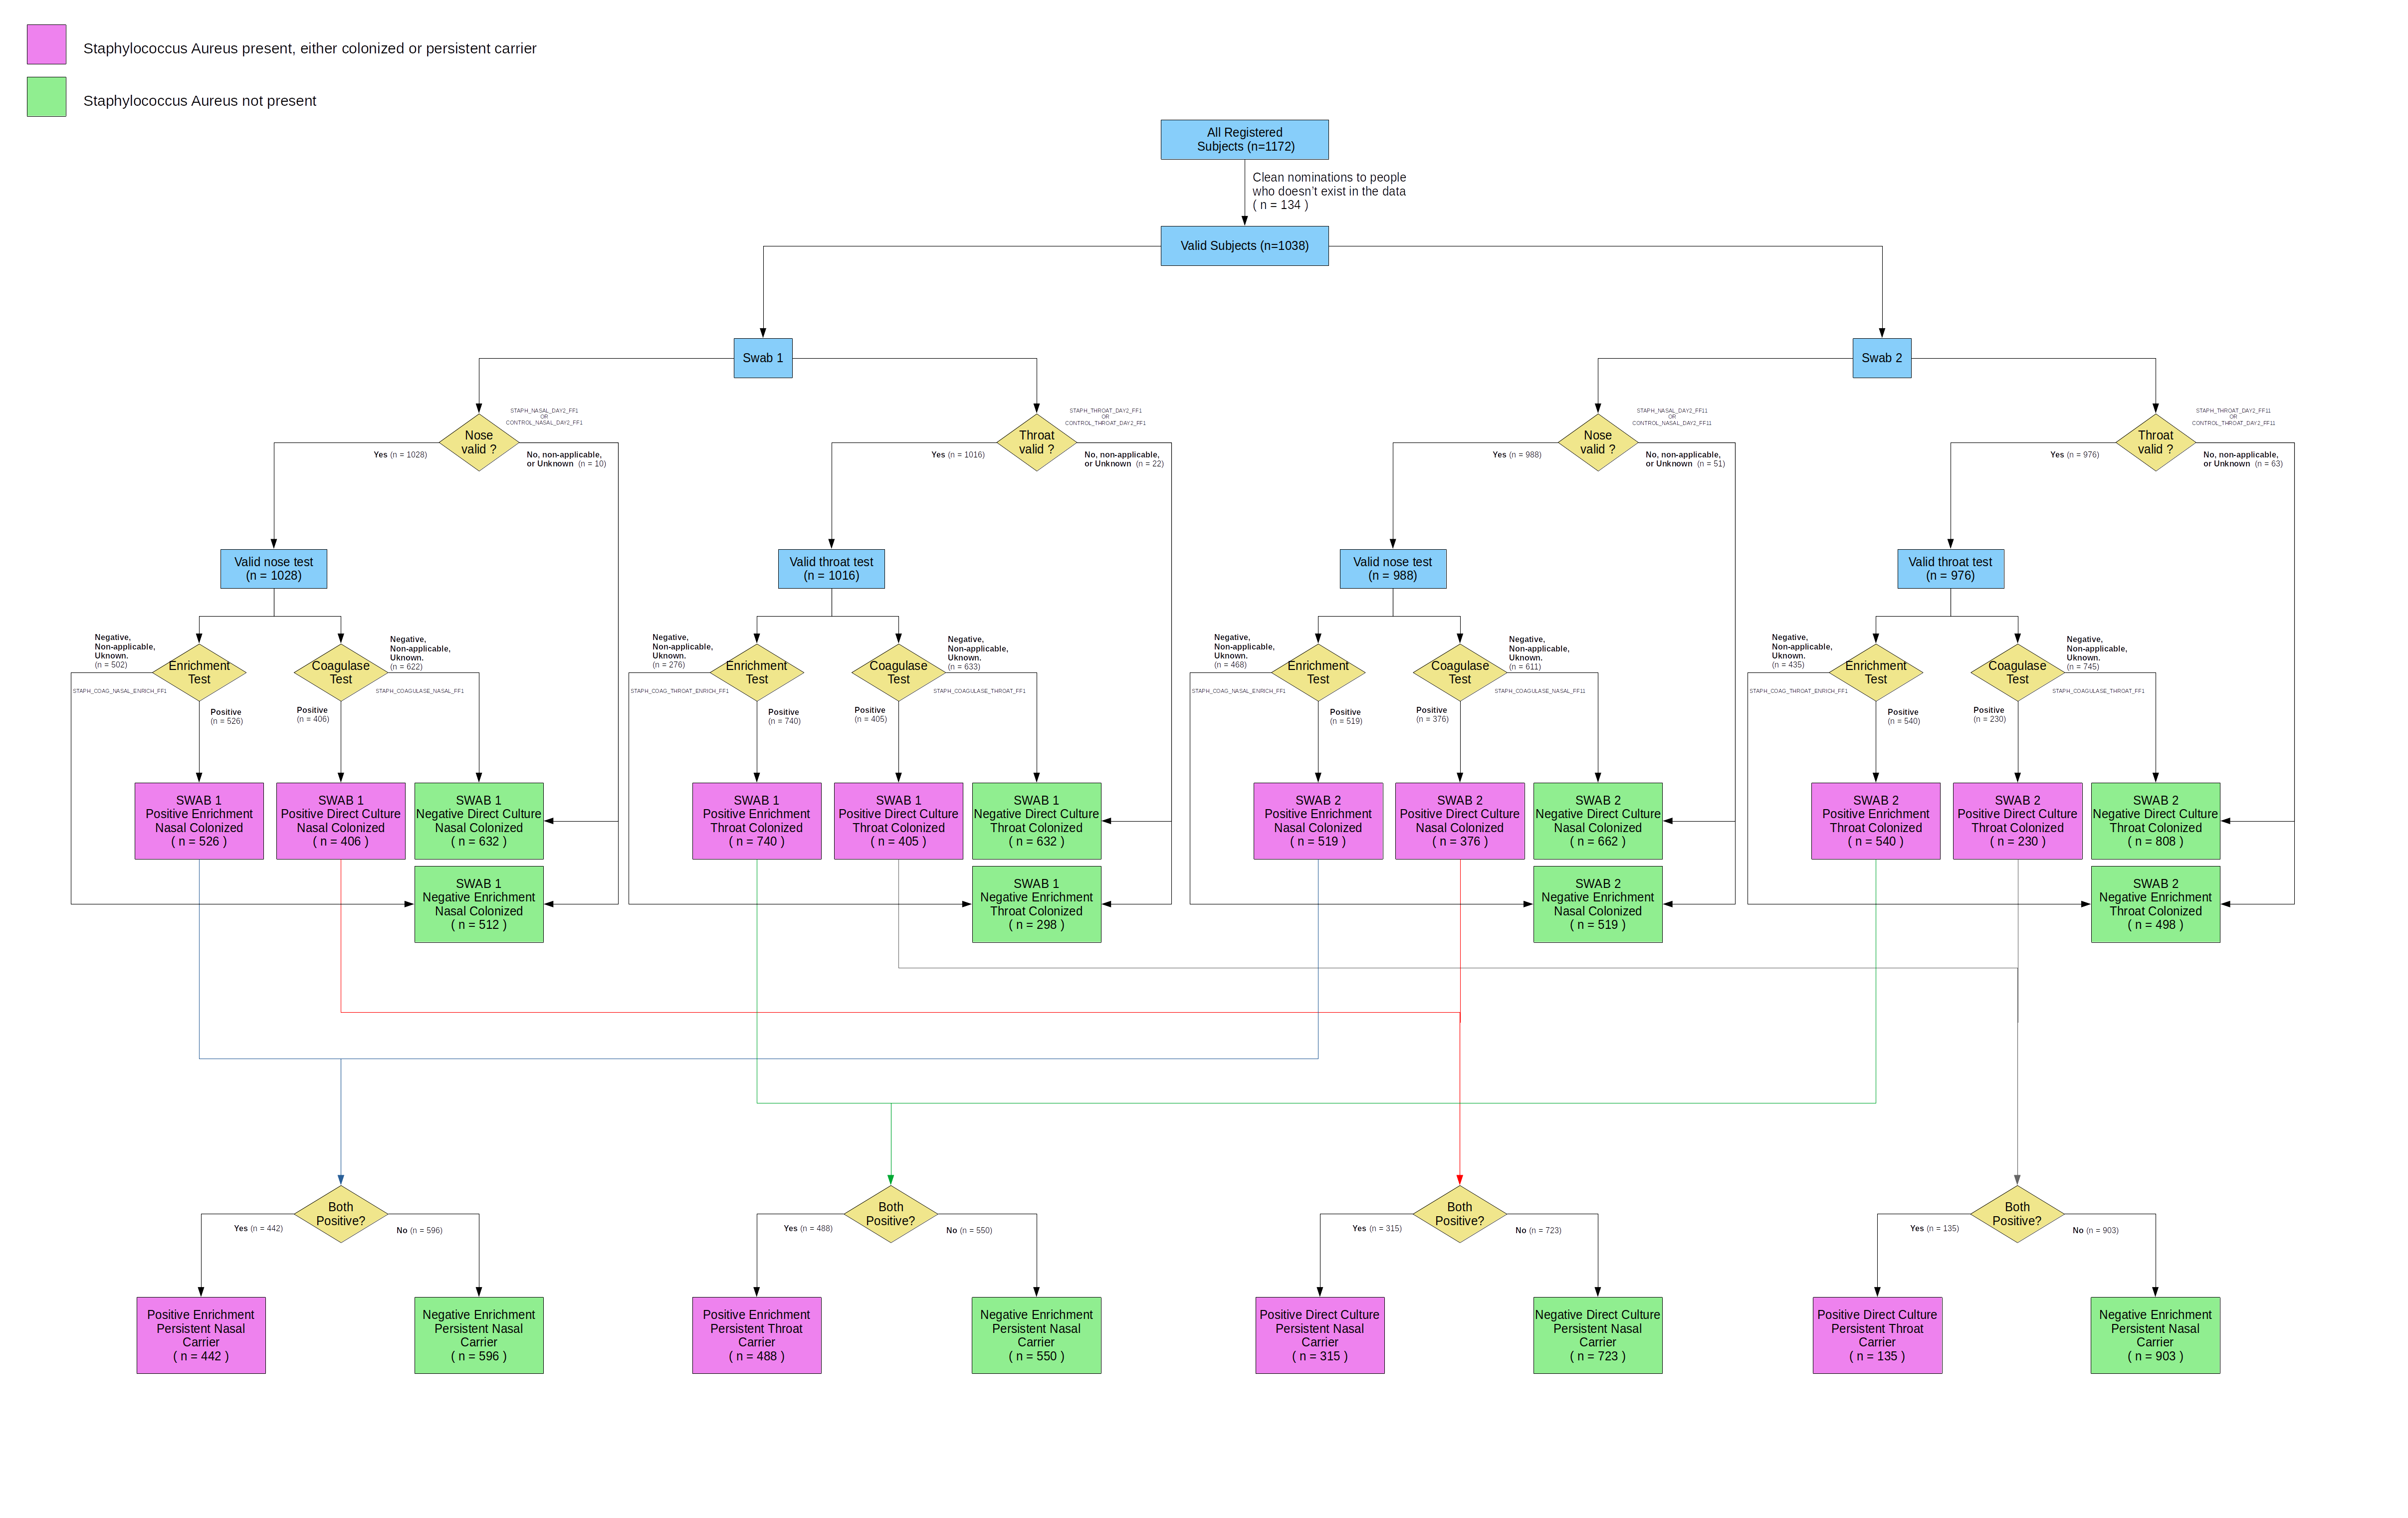
\includegraphics[width=1.2\linewidth, angle=90, origin=c]{figures/Methodology/carrierDefinition.png } 
                \caption{All the S. aureus combinations. A PDF version of this image can be found at the GitHub repository:  \url{https://github.com/rafanozal/PhDThesis/blob/main/Images/carrierDefinition.pdf}}
                
                \label{fig:Carrier_definition}
            \end{figure}

\clearpage

\subsection{Anthropometry assessment}
 
All anthropometric measurements were measured on an electronic scale with participants wearing light clothing and no footwear. BMI is calculated as weight (kg) divided by the squared height ($m^2$) with no correction for sex or age. FF1 has a total of 1034 valid samples, and FF2 has a total of 694.

The BMI comes as a real number and we categorize it following the \gls{who} definition\cite{whoBMI}. "Underweight" if the BMI is lower than 18.5, "Healthy" is above 18.5 and below 25, "Overweight" is between 25 and 30, and "Obese" is greater than 35. The new column is a categorical variable with this information for each person.
  
The WHO also provides BMI-for-age growth charts that take into consideration an individual’s age and sex to determine their BMI percentile. A BMI percentile below the 5th percentile is considered underweight, while a BMI percentile between the 85th and 94th percentiles is considered overweight, and a percentile above the 95th percentile is considered obese. This definition is NOT used since being a relative respects an average rather than a constant value (i.e.: a student being the less obese of a group of people does not make the student not obese); instead, a constant reference point is used as described in the previous paragraph for better comparison across time.

% Describe how does the antropometric variables are measure https://link.springer.com/article/10.1007/s11657-014-0185-0#citeas ; I have no idea why they gave me this reference. Nothing is actually explained there :(

\subsection{Vitamin D assessment}

Blood samples were collected by nurses at the \gls{unn}, centrifugated, and plasma serum was frozen at -70ºC in the Biobank at the \gls{uit}. All samples (n = 890) were sent to the Hormone Laboratory, Haukeland University Hospital, Bergen, Norway; and analyzed by high-pressure liquid chromatography-mass spectroscopy (LC-MS/MS). A sample from all blood vials was reanalyzed at University College Cork, Cork, Ireland, by LC-MS/MS again as a part of the \gls{vdsp} \cite{vdspreference}, and standardization was applied to the rest of the samples \cite{Cashman2015}. 25(OH)D was used as a marker for vitamin D levels. This combines both sources of provitamin D + UVB, and D2+D3 from diet. It has a longer half-life span in blood than other available metabolites. Both 25(OHD)D\textsubscript{2} and 25(OHD)D\textsubscript{3} were measured at the same time. 

\subsection{OLINK Target 96 Inflammation }

Serum levels of 92 proteins were analyzed at the Clinical Biomarkers Facility, SciLifeLab, (Uppsala, Sweden), using the Target 96 Inflammation panel from Olink Holding AB (Uppsala, Sweden) \cite{olinkWeb}. A detailed description of the significance of each marker, alongside the mathematical significance of the values, can be found in the supplementary materials. A total of 936 samples were analyzed this way.

\subsection{Simulations}

\label{sec:MetodologySimulations}


Bootstrapping is a statistical technique used to estimate the variability of a sample statistic without making any assumptions about the underlying population. To determine whether there is bias within the relationships in a network we use bootstrapping simulating 1000 networks using a similar approach to previously described non-parametric tests \cite{ref:nonparametricBook}. This consists of counting how many relationships connect two nodes with the same attributes in our network (i.e., \textit{S. aureus} carrier with \textit{S. aureus} carrier) and comparing this number with the same number given by the simulations. In figure \ref{figure:methodSimulations1} we can see an example of a real network, a simulated one, an arbitrary node attribute distribution, and the same-to-same relationships in each.

    \begin{figure}[H]
        \centering
            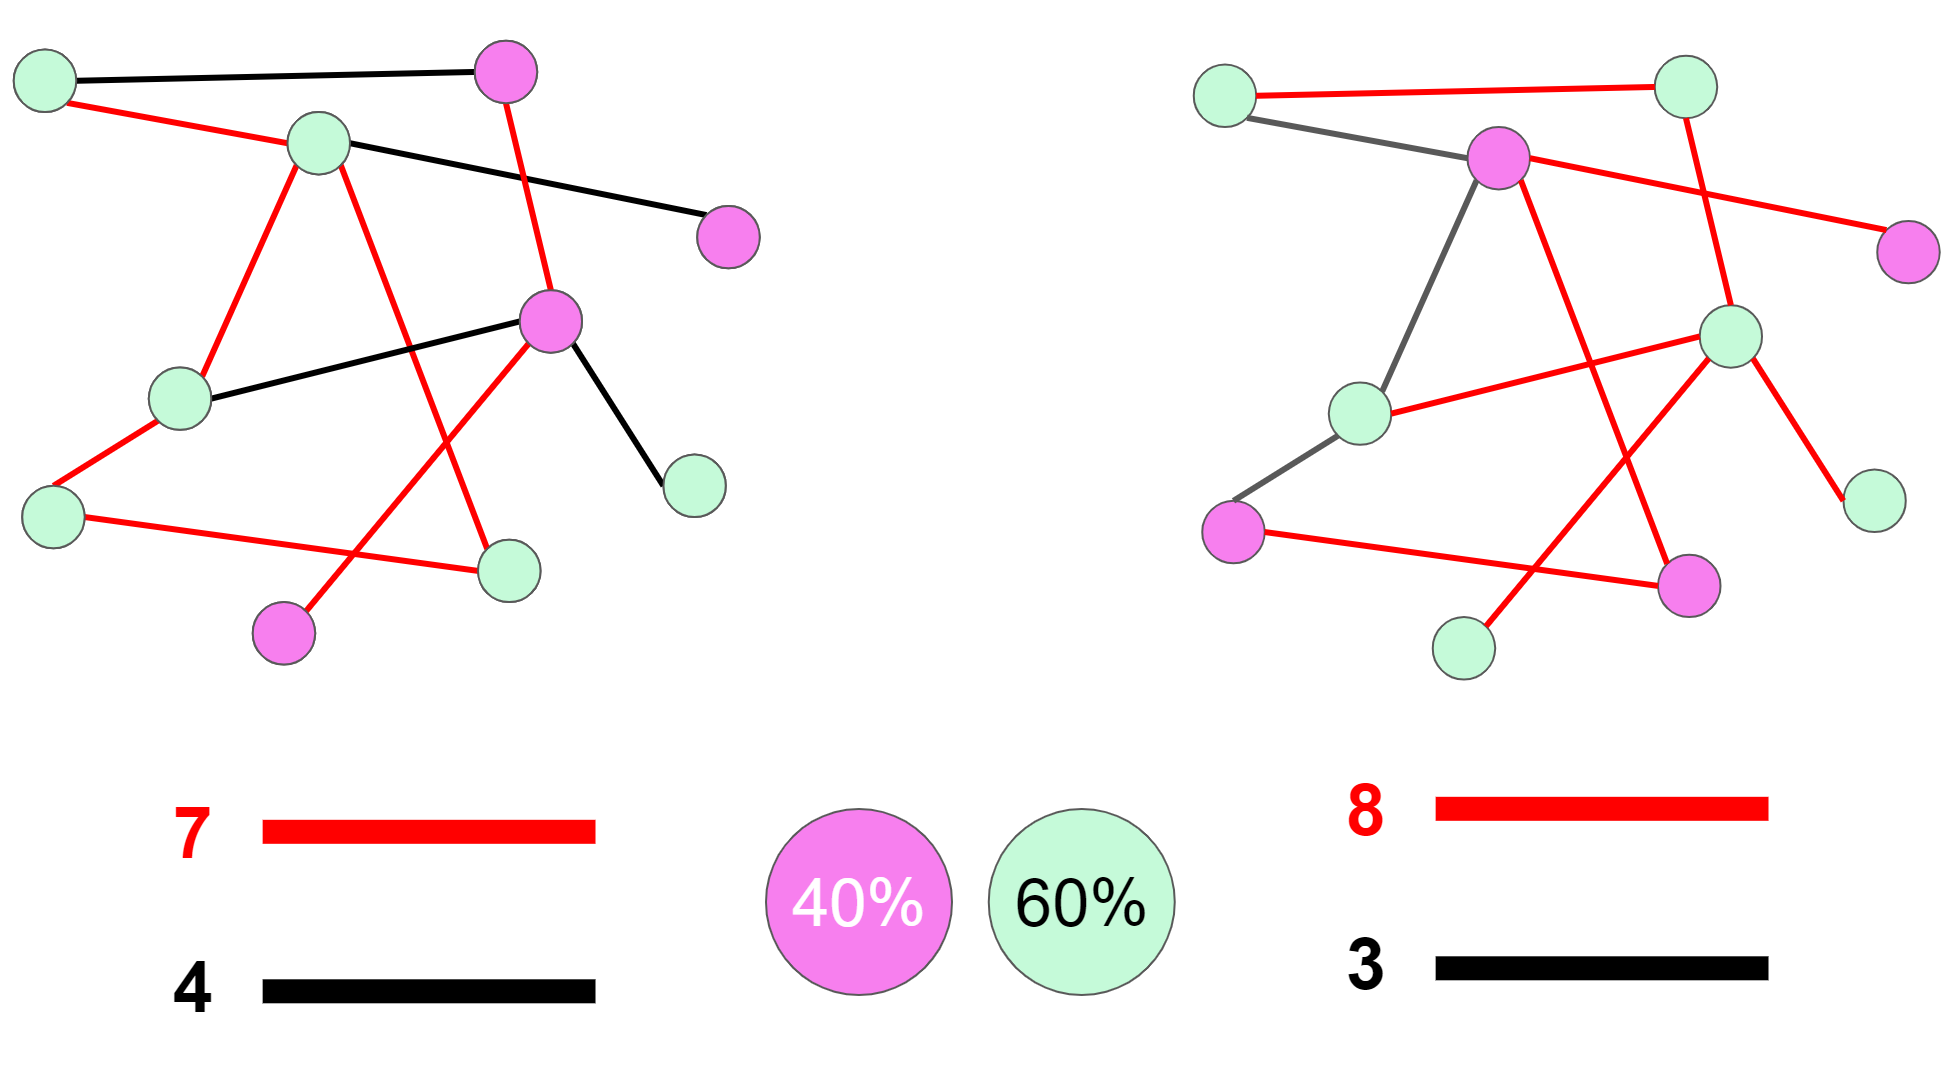
\includegraphics[width=0.7\linewidth]{figures/Methodology/Simulations1.png } 
        \caption{In this figure we see two isomorph networks with the same layout. On the left, we have a representation of a real network. On the right, is a simulated network. Both networks have the same distribution of attributes, with 4 nodes in purple and 6 nodes in green. On the real network, we count 7 edges that share the same node color (same-to-same relationship) which are highlighted in red; while in the simulated network, we count 8. This result indicates that the real network has a bias towards nodes not sharing the same color because the simulation is assumed random and without bias. However, one simulation is not enough, and the result can be due to just random chance. Therefore, the process described on the right is repeated 1000 times, making a distribution of counted same-to-same simulated relationships.}
        \label{figure:methodSimulations1}
    \end{figure}

This gives us a distribution of 1000 values from which we can extract a mean and a standard deviation. We then perform simple hypothesis testing, like a t-test, using the real amount of same-to-same relationships against a normal distribution given by the simulated mean and standard deviation. 

We expand on this concept by instead of using the distribution of attributes in the general population of a node (i.e., \textit{S. aureus} carrier prevalence being 30\%), using the distribution of one specific category (i.e., \textit{S. aureus} carrier prevalence in women being 20\%) and repeating the same process for each category present in each attribute of interest (ie: women and men in sex, from underweight to obese in BMI, and so for). This gives us a new mean which then can be compared with the previous simulated distribution. In this way, we can check how much each of the categories deviates with respect to each other, and we can identify which category has a higher or lower risk for the outcome variable; if any.

Ideally, this technique should be done not by simulating similar networks, but by simulating every possible network and comparing those in which bias happens to those in which bias does not happen. However, it is impossible to find every possible network within reasonable computational time. So we need to reduce the number of possible networks based on some assumptions \cite{Bevan2017}. This allegedly gives the model properties that make it similar enough to all the possible networks. In our case, we use the same frequency tables with a network with the same topology as constriction. We also assume that the virulence of \textit{S. aureus} would cluster carriers with carriers and vice-versa. As BMI homophily is high and the Chi-square table also suggests so, we also assume that this happens with subjects with similar BMI. Finally, we also assume that friends share similar environments and activities and this would be reflected in their vitamin D levels.

\subsection{Friendship ratio}

Biomarkers levels are a continuous variable and as such we cannot use the simulation approach unless we categorize them into something similar to "low level", "medium level", and "high level", losing some information in the process. Instead, we compare numerical levels between friends and non-friends biomarkers one by one. We do this by finding the ratio of, the average square difference between each person's biomarker level and friend's biomarker levels, and the average square difference between each person's biomarker levels and non-friends biomarker levels. Values significantly greater than 1 suggest that clusters of friends have similar biomarker levels in comparison with the rest of the non-friend population, while values smaller than 1 would suggest the opposite. Values similar to 1 suggest nothing, however, we do not know a sensible threshold cut-off for this approach. We arbitrarily suggest that values greater than 1.1 or smaller than 0.9 are the significant ones.

\section{Data cleaning}

\label{datacleaningSection}

%A full report on how the data was transformed, as well as the cleaned data, is available upon request.

This section will present a summary of the important parts of the methodology followed in the data-cleaning process as well as the shortcomings encountered due to the experiment design or the original data-registering process. In the Appendix (chapter \ref{ch:Annex}), some samples from the 25 tables with the original variables' names and a description of what each variable represents are provided, but we do not provide examples from tables that could potentially be used to identify students.

    \begin{figure}[H]
        \centering
            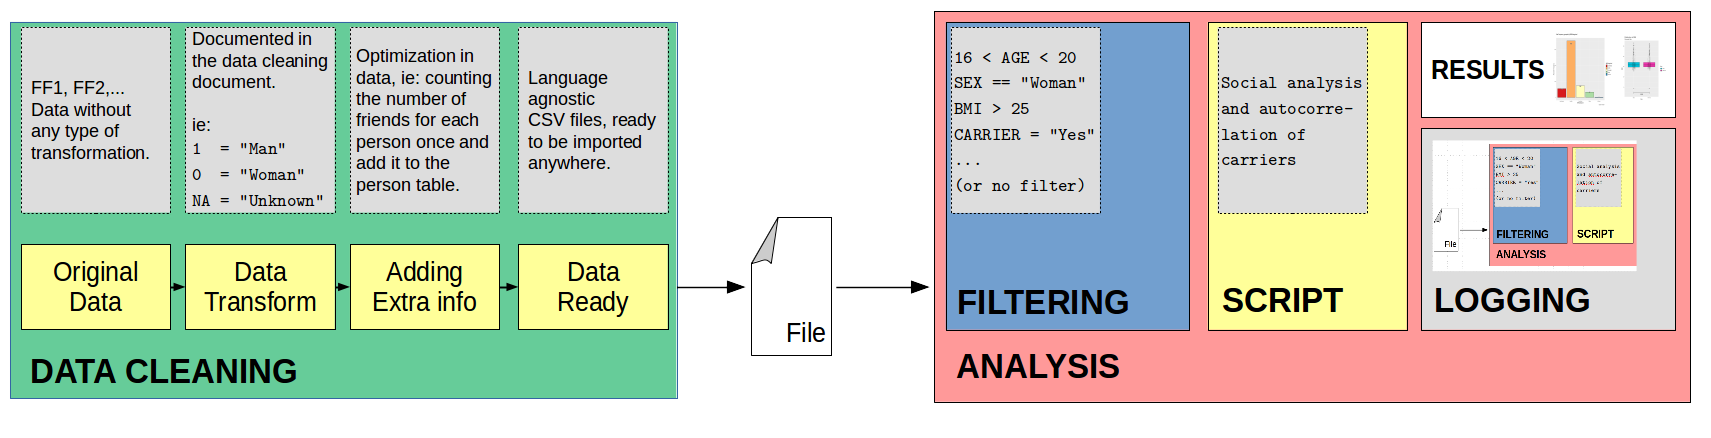
\includegraphics[width=0.95\linewidth]{figures/Methodology/general.png} 
        \caption{Overview of the data cleaning process. To the left, each step that transforms the raw data into a more practical version. This process is done only once. To the right, the subsequent analyses are performed as many times as needed.}
        \label{fig:Data_cleaning_summary}
    \end{figure}

Using our data will save time as it has been thoroughly cleaned, numerical data which is meant to be categorical has been given meaningful strings, diseases with just a verbal description with no code for \gls{icd10} has been assigned manually, and most importantly the data has been transformed into tables following proper Boyce-Codd normalization \cite{ref:KOHLER201888}.


\subsection{Naming}

We changed their name to something more human-friendly and CSV and latex-compatible. This means using upper and lower cases appropriately, "ID" instead of "pers$\_$key$\_$ff1". Samples are labeled as S1 and S2 instead of the given FF11 or FF12 sub-time period. Direct culture and enrichment broth are simplified to "direct" (from STAPH in any case which is confusing) and "enrich". Units are included where possible in the variable name ("FE$\_$FF1" to "Fe$\_$(µmol/L)"). All FF id references are deleted as they are divided into Table$\_$FF1, Table$\_$FF2, and so on. Adding variable name continuity to quickly discern between binary and categorical variables ("FAT$\_$FISH$\_$FF1" to "FatFishFrequency") so the user already knows what to expect in each column. Deleting redundancy in names (  "FRIEND2$\_$CONTACT$\_$SCHOOL$\_$FF1" to "Friend2School").

\subsection{Dates}

For all tables where a date appears, dates are standardized from several data formats (Posix, "mm/dd/YY", "dd/mm/YY", "YYYY-MM-DD") to "YYYY-MM-DD" format. Some of the dates could be transformed to have more precision down to "HH:mm:ss" resolution, but this information is irrelevant to us anyway so it is discarded. SPSS is the programming language that is used to encode the original data, and it uses the start of the Gregorian Calendar in 1582 as the default date for POSIX origin. Because of this chosen date reference, there might be some days' error in coercion in these dates because we do not know which timezone, or time origin, we take as a reference. We delete all timezones from UTC to simply a date, which we assume is GMT +1/+2 depending on the time of the year. Since the time difference is one to two hours, and we have a day resolution level, this loss of detail does not matter. It is advisable to use another non-SPSS method in the future as this time error coercion might render biological data which is time-critical unusable.

\subsection{General tables}

\subsubsection{\textit{S.aureus}}

These tables contain the \textit{S.aureus} information. Note that none of the FF11 variables are described in the metadata files. The information was retrieved from Fit Future experiment designers.

\subsubsection{Swabbing information}

All lab comments that are just registered as \textit{"OK"} by lab technicians for all samples are discarded to avoid data redundancy. Also, all status and event variables are redundant information and are later discarded. All leading and trailing white spaces are deleted. None of these variables are described in the metadata and information.

What remains, for each unique nasal and throat swab, is whether the swabbing was performed successfully, with irregularities and the given reason, the swab was repeated, or the swab was not performed at all. We also have the freezer ID of where to find each sample as well as the freezing date.

\subsubsection{Blood serum and Blood Technical information}

Several variables indicate if some value is above or below the healthy limit which are discarded. The reference on whether some value is healthy or not is marked during the analysis according to the given references for each value. Within the blood serum scope, there are also a bunch of columns named EVENT0 to EVENT9, and EVENTA to EVENTL, which are empty, no description is given in the metadata or any other source, and have no information at all. As such all of them are deleted. All LCMSMS (Mass spectrometry measures) have the same values as their normal measurements counterparts, so those are also skipped.

\subsection{Relational Normalization}
\label{ssec:normalization}

The original data does not have any type of relational meaning between columns. To add future benefits, we need to fix this issue due to privacy security \cite{DomingoFerrer2009}, data logical consistency \cite{DomingoFerrer2009}, and computational time efficiency. This section describes all tables related to relational data. The medicine, contraceptive, and disease tables are read from the original dataset and then transformed later into a structure that follows a proper relational database property.

%\subsection{Formatting}

%In the previous section, we have described which type of data is available to us. Here we are going to explain how the data is clean and transformed into something more useful. The process consists of importing the data from the files described previously with no type of filter. Then transform the original data into values that are more meaningful, as well as add new columns to our data based on data that we already have (i.e.: whether a person is \textit{S. aureus} carrier or not). Then prepossessing the data and adding columns that are time intensive (i.e.: searching for all the friends for all the people, and counting how many types of relationships they have, takes a lot of computational time when you have to do it thousands of times, but you don't need to do this every time you run the network analysis). Finally, we need to normalize the diseases and medicine tables into a proper relational structure. Same for the contraceptive table which is a special case of the medicine table.

%After all of these steps, the data is finally clean and ready to use. But we don't use the data just yet. We save this final version into CSV files and later on we apply the filtering variables with whatever restrictions you want (i.e.: age from 15 to 18). This way, the data cleaning, filtering, and analysis are independent of each other. Notice that data stratification happens where needed during the analysis (i.e.: table for women and table for men); this operation is always O(n) and doesn't need a lot of time to be carried on as it doesn't need to transform all the graphs regarding friendship again and again.


%In all cases, first, we are going to change the selected variable names to something more meaningful; the same for the categorical values that are encoded as numbers.

%\subsubsection{Naming}

%All the variables that we named in the previous chapter changed their name for something more human-friendly and CSV and latex-compatible. This means using upper and lower cases appropriately, "ID" instead of "pers$\_$key$\_$ff1". Samples are labeled as S1 and S2 instead of the given FF11 or FF12 sub-time period. Direct culture and enrichment broth are simplified to "direct" (from STAPH in any case which is confusing) and "enrich". Units are included where possible in the variable name ("FE$\_$FF1" to "Fe$\_$(µmol/L)"). All FFX references are deleted as they are divided into Table$\_$FF1, Table$\_$FF2, and so on; since are implicitly declared at the table level the extra characters are redundant at the variable level. Adding variable name continuity to quickly discern between binary and categorical variables ("FAT$\_$FISH$\_$FF1" to "FatFishFrequency") so you already know what to expect in each column. Deleting redundancy in names (  "FRIEND2$\_$CONTACT$\_$SCHOOL$\_$FF1" to "Friend2School").

\label{relationalNormalization}
%\subsubsection{Relational Normalization}

The data should be organized in Boyce–Codd normal form \cite{ref:KOHLER201888}. Boyce-Codd normalization is important because it ensures that there are no data dependencies between columns, which translates into guaranteeing the integrity and consistency of data which is critical for accurate analysis. This is also crucial in datasets with large amounts of data, but this is not the case. Summarizing the normalization process, all variables and data in those tables need to be transformed so they follow these fundamental principles of normalization:

\begin{itemize}

    \item \textbf{0NF} No information is lost and no information is duplicated.
    \item \textbf{1NF} No columns, or multicolumns (3NF), which contain sets of values.
    \item \textbf{2NF} Single column primary key (person ID) which is also used as superkey (4NF).
    \item \textbf{3NF} Eliminating the transitive functional dependencies.
    \item \textbf{BCNF} Always satisfies lossless join condition.

\end{itemize}

\begin{figure}[H]
        \centering
            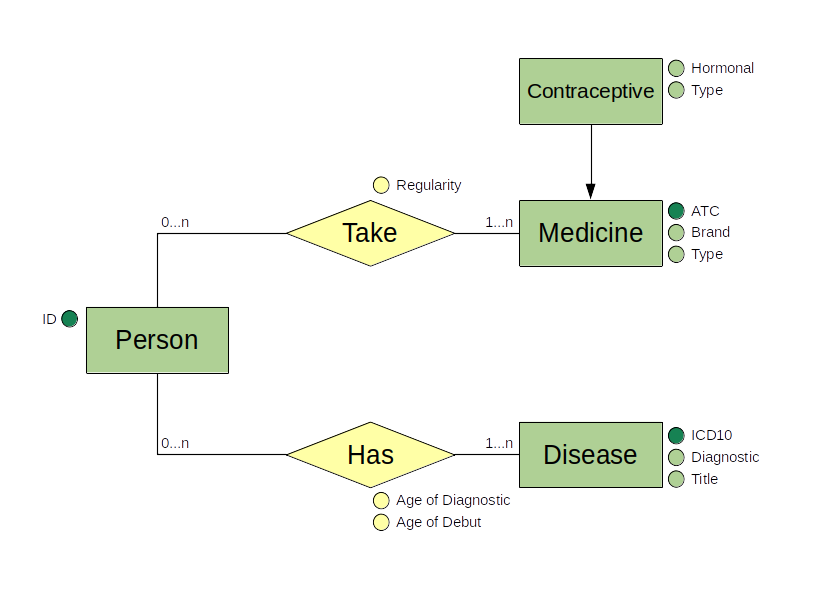
\includegraphics[width=0.75\linewidth]{figures/Methodology/DBrelationals.png} 
        \caption{BCNF transformation from the original data. The database schema for "Person" can be obtained upon request.}
        \label{fig:Database_relational_image}
\end{figure}

%Further information about what compromises the "person" table can be found in the appendix, in section \ref{chapter:Annex_schema}.

%In other tables, similar transformations are produced. Which we will see one by one in the next section. However, because this dataset is not especially big, we applied the join operations to all tables and saved the result in our files. This actually fails the non-duplicity condition and increase significantly the CSV file size, but we do it anyway to increase performance in R (which otherwise would be quite slow having to do joining operations over and over). The disjoint operation is quite trivial if needed (just unique by ID and ICD10, and ID and ATC). The final results for the diseases, medicine, and contraceptive tables, are as follows:

%\begin{table}[H]

	%\tiny	

    %\centering

    %\label{table:Diseases_DB}
    
	%\renewcommand{\arraystretch}{1.5}

    %\begin{tabular}{| l | p{10cm}  l }
     %   \hline
      %  \rowcolor[HTML]{FFAAAA}

       % \textbf{Name} & \textbf{Description} \\ 
        %\hline 

        %\multicolumn{1}{l|}{\detokenize{ID}}             & Person ID \\ 
        %\multicolumn{1}{l|}{\detokenize{Diagnostic}}     & Name of the disease \\ 
        %\multicolumn{1}{l|}{\detokenize{ICD10}}          & Disease identifier following ICD10 \\ 
	    %\multicolumn{1}{l|}{\detokenize{Title}}          & Group to which the disease belongs ("Skin and subcutaneous tissue", "Respiratory system"...) \\
        %\multicolumn{1}{l|}{\detokenize{Age_Diagnostic}} & At what age where you diagnose for the first time \\ 
        %\multicolumn{1}{l|}{\detokenize{Age_Debut}}      & At that age where the symptoms first appeared \\ 

    %\end{tabular}%

    %\caption{Table with the final disease variables in relational format.}
    
%\end{table}

%\begin{table}[H]

	%\tiny	

    %\centering

    %\label{table:Medicine_DB}
    
	%\renewcommand{\arraystretch}{1.5}

    %\begin{tabular}{| l | p{10cm}  l }
     %   \hline
      %  \rowcolor[HTML]{FFAAAA}

       % \textbf{Name} & \textbf{Description} \\ 
        %\hline 

        %\multicolumn{1}{l|}{\detokenize{ID}}         & Person ID \\ 
        %\multicolumn{1}{l|}{\detokenize{Type}}       & Group of the medicine ("Antiinfectives for systemic use", "Genito-urinary system and sex hormones")\\ 
        %\multicolumn{1}{l|}{\detokenize{Brand}}      & Name of the medicine ("Ery-Max", "Microgynon", "Paracetamol", "Ibux 400 mg") \\ 
	    %\multicolumn{1}{l|}{\detokenize{ATC}}        & Medicine ID following the ATC codes.\\
        %\multicolumn{1}{l|}{\detokenize{Regularity}} & How often do you use it \\ 

    %\end{tabular}%

    %\caption{Table with the final medicine variables in relational format.}
    
%\end{table}

%\begin{table}[H]

	%\tiny	

    %\centering

    %\label{table:Contraceptives_DB}
    
	%\renewcommand{\arraystretch}{1.5}

    %\begin{tabular}{| l | p{10cm}  l }
     %   \hline
      %  \rowcolor[HTML]{FFAAAA}

       % \textbf{Name} & \textbf{Description} \\ 
        %\hline 

        %\multicolumn{1}{l|}{\detokenize{ID}}         & Person ID \\ 
        %\multicolumn{1}{l|}{\detokenize{Brand}}      & Name of the medicine ("Microgynon", "Cerazette") \\ 
	    %\multicolumn{1}{l|}{\detokenize{ATC}}        & Medicine ID following the ATC codes.\\
        %\multicolumn{1}{l|}{\detokenize{Type}}       & Contraceptive type ("Subdermal", "Oral", "Condoms")\\
        %\multicolumn{1}{l|}{\detokenize{Hormonal}}   & Type of hormone used ("Non-hormonal", "Progestin", "Low Estradiol" )\\ 

    %\end{tabular}%

    %\caption{Table with the final contraceptives table in relational format.}
    
%\end{table}

%There is further transformation to individual data cells in these tables that has nothing to do with the normalization process (ie: translating from Norwegian or standardizing disease names), or defining which type of hormonal contraceptive each brand medicament belongs to.

\subsection{IDs transformation}

Each individual has a personal key described in the \detokenize{"pers_key_ff1"} variable. The original key looks like this: "12345678" and is simply an 8-digit unique key for each of the 1038 individuals in that file. To avoid visual cluttering and math optimization, we substitute the original IDs with an integer number that goes from 1 to 1038, assigned randomly to each individual.

We have two special IDs. An ID equal to 0 means that a person has a friend that is not in our ID table, for example, it could be a student in another school that is not in Tromsø, or Balsfjord; in short, people who were not part of this study. An ID equal to -1 means no friend. This ID numbering keeps consistency later on when we do the filtering. This way, all the variables for each of the 5 friends have an integer, and is easier and faster to do math, indexing, and filtering. ID swapping log is registered in case identifying the original person is necessary but kept confidential.

%In this process of deleting people who are "unknown", we also delete friendship nominations from people who are registered towards people who are unknown. We don't know how many nominations are from people who are unknown to people who exist because we haven't asked those people who are their friends, so the original number of nominations and how many we lost is impossible to calculate. We can tell however how many nominations we have between people who are registered, plus the nomination from registered to unknown (with unknown to registered missing)

%This is the summary of nodes and edges lost in this process:


%\begin{table}[H]
 %   \centering

  %  \resizebox {0.5\textwidth}{0.1\textheight}{ 

% 	\renewcommand{\arraystretch}{1.5} 
 %   \begin{tabular}{ lll }
  %      \hline
   %     \rowcolor[HTML]{FFFFC7}

    %     \textbf{ Concept } &         \textbf{ Total } &         \textbf{ Relative } \\ 
     %   \hline 

      %  \multicolumn{1}{l|}{ Total IDs: } & 1177   & 100 \%          \\ 
       % \multicolumn{1}{l|}{ - Total Deleted IDs: } & 139   & 11.81 \%          \\ 
        %\multicolumn{1}{l|}{ - Total Remaining IDs: } & 1038   & 88.19 \%          \\ 
%        \multicolumn{1}{l|}{ Total Edges: } & 4125   & 100 \%          \\ 
 %       \multicolumn{1}{l|}{  - Total Deleted Edges: } & 473   & 11.47 \%          \\ 
  %      \multicolumn{1}{l|}{  - Total Remaining Edges: } & 3652   & 88.53 \%          \\ 

    %\end{tabular}
 %} 
 
    %\caption{Summary of lost connections at data cleaning.}
    %\label{table:SummaryLost}

%\end{table}

%\begin{figure}[H]
 %       \centering
  %          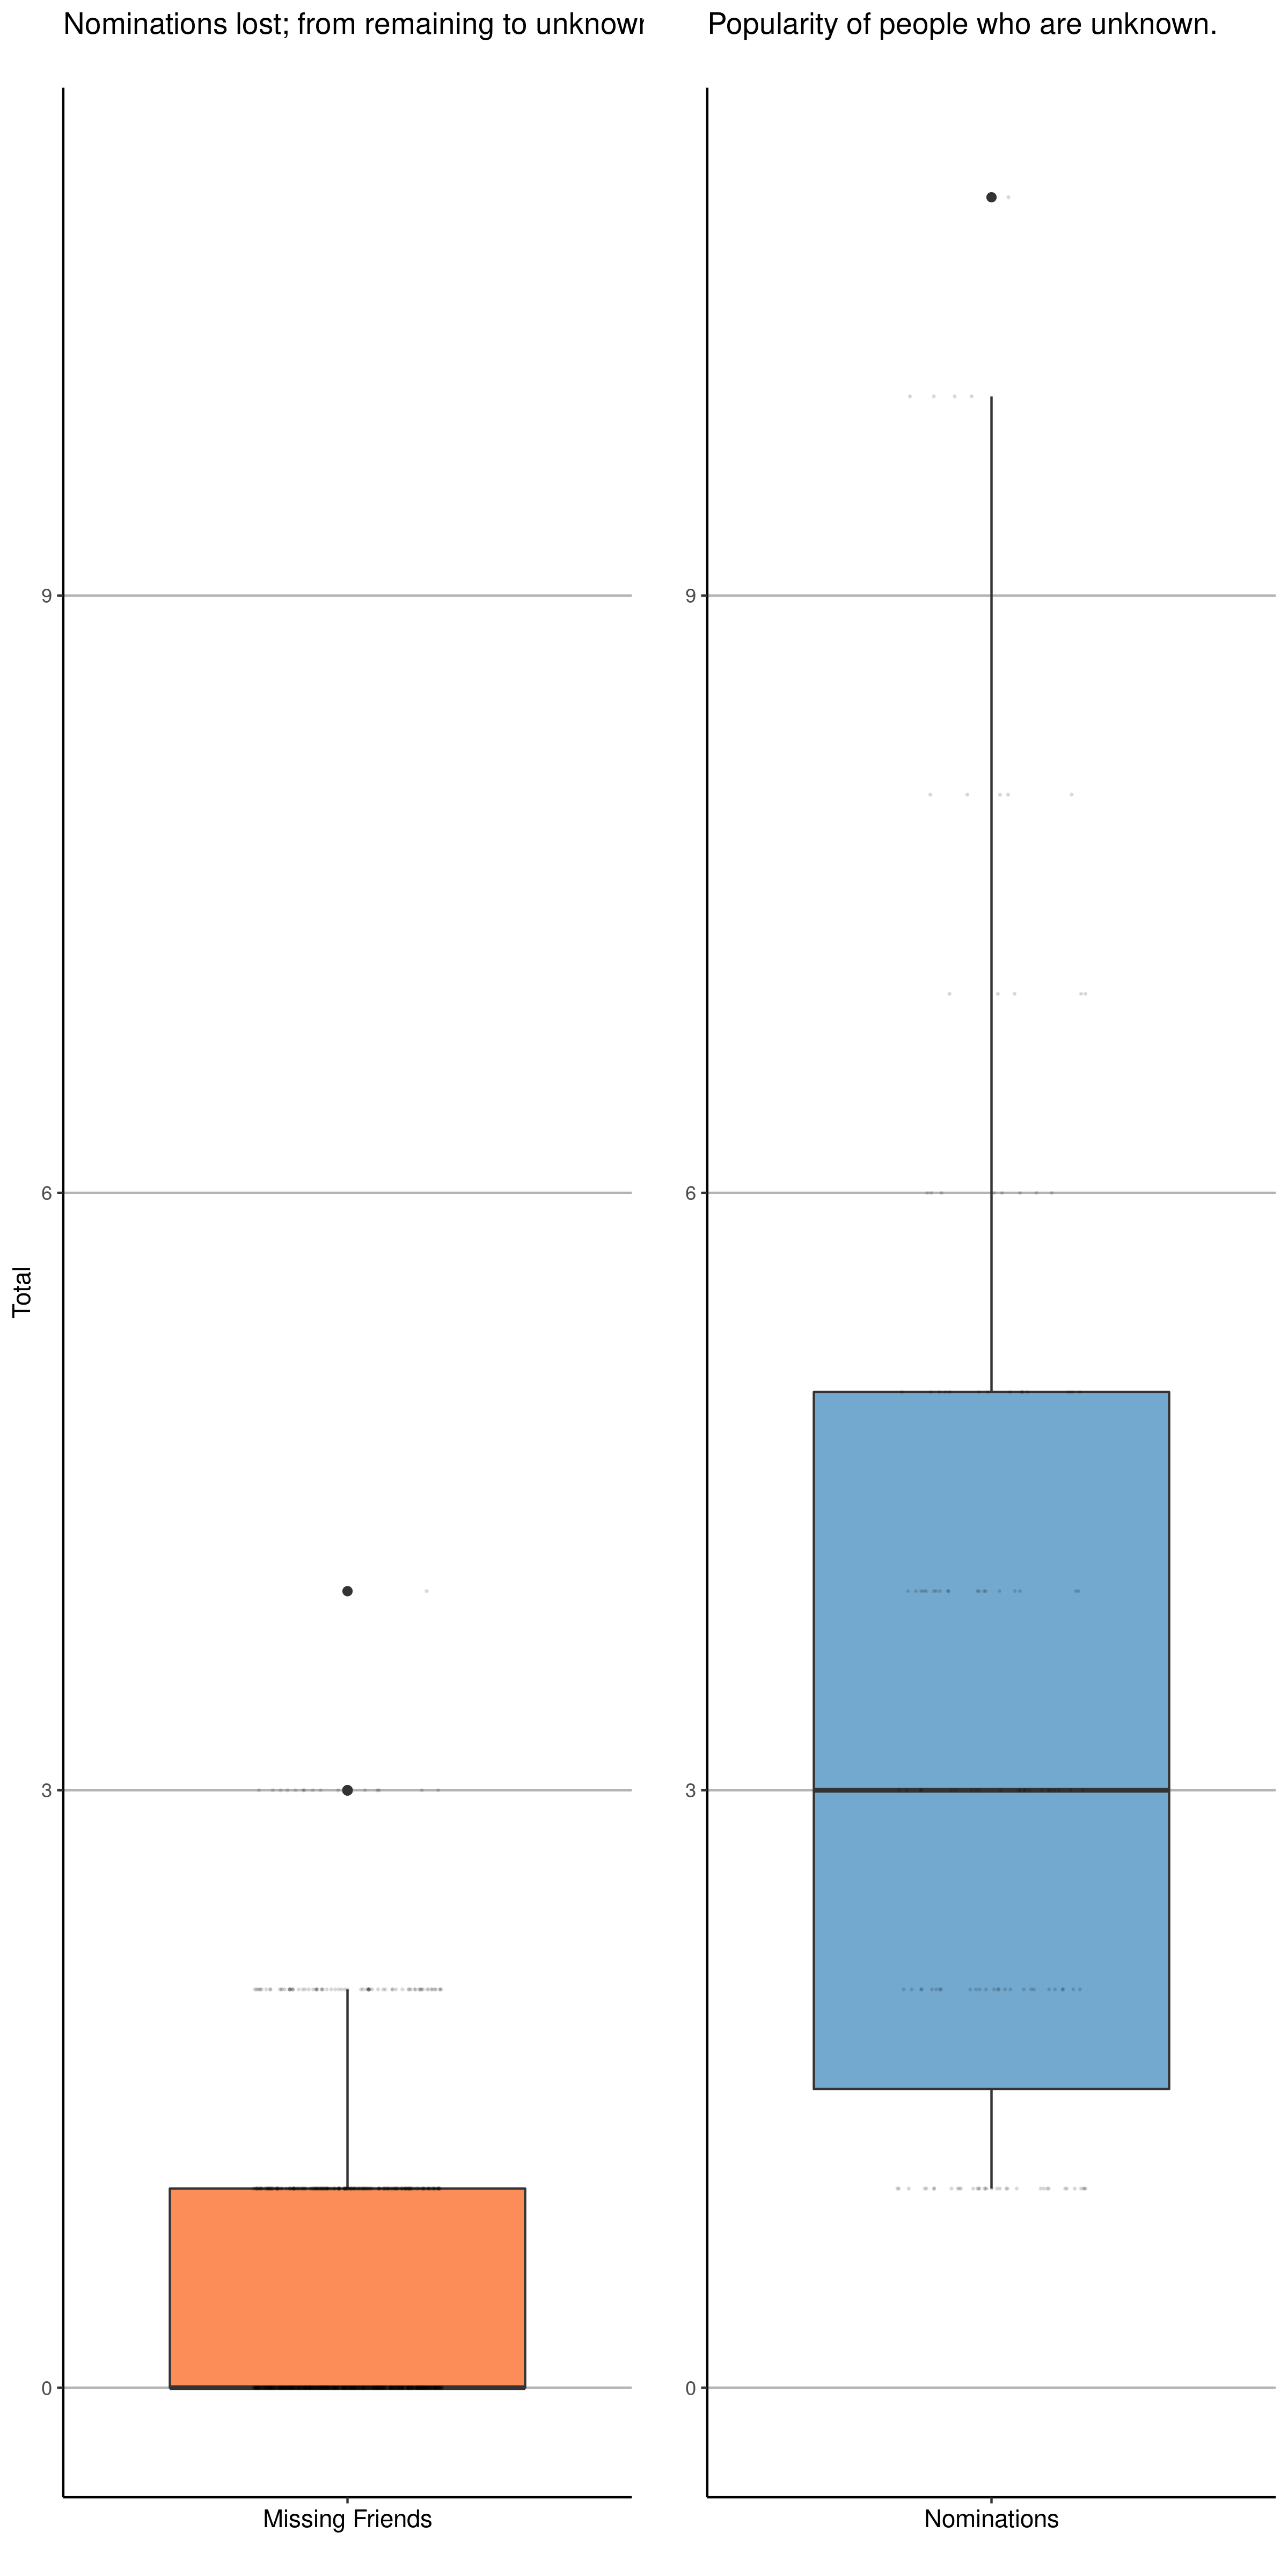
\includegraphics[width=0.2\linewidth]{figures/Methodology/NominationsBoxplots.png} 
   %     \caption{Summary of all nominations lost}
    %    \label{fig:boxplotLostNominations}
%\end{figure}

\subsection{Mapping}

In this subsection, we discuss the relevant issues that arise during the mapping and transformation of the original variables. From the subsequent 29 tables generated during the mapping, we only provide a few relevant examples in this thesis.

\subsubsection{\textit{S. aureus}}

Changes for Nasal and Throat variables are identical. This is also true for the variables for sample 1 and the variables for sample 2. In total, we have Nasal Sample 1, Nasal Sample 2, Throat Sample 1, and Throat Sample 2. Notice that all SPA-type variables remain the same.

\subsubsection{School and education}

Three columns represent "HighSchool", "Class", and "Programme". All of those have a numerical ID to represent the high school, a numerical ID to represent each class, and so on. While those can work ok the way they are, I choose to change them by adding a letter to each column to categorize it properly; these are not numerical values, these are categories. So high-school "1" becomes "H1", high-school "2" becomes "H2", class "10" becomes "C10", program "23" becomes "P23", and so for all values.

\subsubsection{Sociology}

Two variables expressed if "You live with 1 to 2 Siblings (yes/no/NA)", and "You live with 3 or more siblings (yes/no/NA)". Ideally, the questions should be: "How many siblings do you have? (number)", "How many siblings live with you? (number)". But we do not have that. However, we can convert those two variables into a single categorical variable that is expressed as "How many siblings live with you? (NA / Zero / One or Two / Three or more)". Regarding working status, the original data is also divided into too many variables that should not be, as they are sometimes mutually exclusive. The first one is "Is your mother studying?", "Is your mother a housewife?", and "Is your mother disabled?". All three of those are okay to have them separated as any combination of those (yes/no), plus working status, is possible. The rest of the possible answers refer to "Full time", "Part-time", "Unemployed", "Pensioned", "Deceased", "Don't Know", and "Other". All of those are grouped into the same variable within the same variable. Regarding ethnicity, the original question is not clear, and people have not answered ethnicity directly; instead, they have a combination of their country of origin, country of residence, country of parents, and their own race or cultural background. So here is the attempt to clear all that data into something useful. The final variable is a string with as many ethnicities as needed ("Norwegian", "Norwegian-Sami", "Belgium-Spain-France"). People who said they are Norwegian, Sami, or Kven, have a combined ethnicity if answered more than one of those, and also combined with whatever they write in the "Other" column where applicable.

We must express our concern that sharing the precise text from the "Other" category may lead to the identification of individuals. Researchers seeking access to the FF data can, however, apply for access to obtain the exact methodology. 

%People who already answered "Norwegian", "Sami", or "Kvensk" and not included in the "Other" translation if they also include one of those three in the "Other" field. People who emphasize they are from North Norway keep their Norwegian ethnicity (3). People who write "fjellfin" are set to "Sami" instead (2). People who are joking or write some invalid text do not get any follow-up ethnicity (1).

Finally, we have these variables which are just a straightforward mapping \textit{"Who do you live with? / What is your parents' educational background?"} In this case, while would be a fringe case, is possible to live with multiple combinations of these at the same time. For example, parents can be divorced while the student lives with both of them half of the time, each having a stepmother/stepfather, while the grandfather also lives inside one of the houses. So all of these variables are kept independent.


\subsubsection{Puberty and Sleeping}

These tables and serve as an example in which categorical data is overdone due to the string field limitations of SPSS/STATA data. 

The variable for "At what age did your pubic hair start growing?" is, originally, saved as a categorical variable, that gets the values "1", "2", "3", "4", "5", "6", "7", that means from 9 to 15 years accordingly. This is changed from a categorical to a numerical value, however, the data is of course censored to the left and to the right since we do not have any other option. Ideally, we should have a real number instead of the category. For the rest of the men variables we have standardized all answers and eliminated references to the variable in each of the options, so instead of "Facial hair has not yet started growing", or "Voice has not yet started changing", both are mapped to "Haven't Started".

In table \ref{table:Table_Sleeping_Mapping} we see that modeling a time of the day, into 18 different categories is not practical. A better solution would be, at the questionnaire level, to ask "At what time do you go to sleep?" so we can have a numerical value instead. This particular mapping is later transformed into "How many minutes since noon passes until sleeping time", which is a more sensible data format.

\begin{table}[H]

    \caption{Original values for the sleeping habits.}

	\tiny

	\centering

    \label{table:Table_Sleeping_Mapping}
    
	\renewcommand{\arraystretch}{1.5}

    \begin{tabular}{l | l | l}
		\hline
        \rowcolor[HTML]{FF9999}		
		
        \textbf{Variable} & \textbf{Original} & \textbf{Transformed} \\ 		
        
        \hline 
                                  
            \multirow{5}{*}{SleepingPills}
                            
            	& \multicolumn{1}{l}{1}     & \multicolumn{1}{l}{Not used}                 \\\cline{2-3}
                & \multicolumn{1}{l}{2}     & \multicolumn{1}{l}{Less frequently than every week}   \\\cline{2-3}
				& \multicolumn{1}{l}{3}     & \multicolumn{1}{l}{Every week, but not daily} \\\cline{2-3}
				& \multicolumn{1}{l}{4}     & \multicolumn{1}{l}{Daily}   \\\cline{2-3}
				& \multicolumn{1}{l}{NA}    & \multicolumn{1}{l}{Didn't Answered}              \\\hline                                                                                                
   
            \multirow{18}{*}{BedTimeHourCat}
                            
            	& \multicolumn{1}{l}{1}     & \multicolumn{1}{l}{18:00 or earlier}                 \\\cline{2-3}
                & \multicolumn{1}{l}{2}     & \multicolumn{1}{l}{18:30}   \\\cline{2-3}
				& \multicolumn{1}{l}{3}     & \multicolumn{1}{l}{19:00} \\\cline{2-3}
				& \multicolumn{1}{l}{4}     & \multicolumn{1}{l}{19:30}   \\\cline{2-3}
            	& \multicolumn{1}{l}{5}     & \multicolumn{1}{l}{20:00}                 \\\cline{2-3}
                & \multicolumn{1}{l}{6}     & \multicolumn{1}{l}{20:30}   \\\cline{2-3}
				& \multicolumn{1}{l}{7}     & \multicolumn{1}{l}{21:00} \\\cline{2-3}
				& \multicolumn{1}{l}{8}     & \multicolumn{1}{l}{21:30}   \\\cline{2-3}
            	& \multicolumn{1}{l}{9}     & \multicolumn{1}{l}{22:00}                 \\\cline{2-3}
                & \multicolumn{1}{l}{10}    & \multicolumn{1}{l}{22:30}   \\\cline{2-3}
				& \multicolumn{1}{l}{11}    & \multicolumn{1}{l}{23:00} \\\cline{2-3}
				& \multicolumn{1}{l}{12}    & \multicolumn{1}{l}{23:30}   \\\cline{2-3}
            	& \multicolumn{1}{l}{13}    & \multicolumn{1}{l}{00:00}                 \\\cline{2-3}
                & \multicolumn{1}{l}{14}    & \multicolumn{1}{l}{00:30}   \\\cline{2-3}
				& \multicolumn{1}{l}{15}    & \multicolumn{1}{l}{01:00} \\\cline{2-3}
				& \multicolumn{1}{l}{16}    & \multicolumn{1}{l}{01:30}   \\\cline{2-3}															& \multicolumn{1}{l}{17}    & \multicolumn{1}{l}{02:00 or later}   \\\cline{2-3}								
				& \multicolumn{1}{l}{NA}    & \multicolumn{1}{l}{Didn't Answered}              \\\hline                                                                                                

        \end{tabular}

    

\end{table}

\subsection{Diseases}

All diseases are transformed into the proper relational table described earlier in section \ref{ssec:normalization}. There are plenty of transformations that need to be curated manually.

\subsubsection{Common Diseases I}

The questionnaire keeps track of diseases in three different ways. First, there are 7 diseases that the original data track explicitly, but do not register any ICD10 code. Those are "Diabetes" (unspecified which type), "Ichy Skin", "Hand Eczema", "Rhinitis", "Asthma", "Atopic Eczema" and "Psoriasis". The ICD10 codes can be seen in table \ref{table:Table_Common_Diseases}.

\begin{table}[H]

    \caption{Table with the common 7 chronic diseases asked in a subsection of the questionnaire.}

	\tiny

	\centering

    \label{table:Table_Common_Diseases}
    
	\renewcommand{\arraystretch}{1.5}

	\begin{tabular}{|llll|}
		\hline
		\rowcolor[HTML]{FFAAAA} 
		Questionary   & Medical                        & ICD10 & Comment                                         \\ \hline
		
		Diabetes      & Other specified diabetes mellitus & E13   &  \\
		Ichy Skin     & Pruritus, unspecified          & L29.9 &                                                 \\
		Hand Eczema   & Dyshidrosis                    & L30.1 &                                                \\
		Rhinitis      & Allergic rhinitis, unspecified & J30.9 &                   \\
		
		Asthma        & Asthma                         & J45.9 &                                                 \\
		Atopic Eczema & Atopic dermatitis, unspecified & L20.9 & Skin and subcutaneous tissue                    \\
		Psoriasis     & Psoriasis, unspecified         & L40.9 &  \\ \hline
		
	\end{tabular}
	
\end{table}

\subsubsection{Common Diseases II}

The second way to track diseases is that during the interview, the student can tell up to 5 chronic diseases, and the ICD10 code is also registered by the person performing the interview. Again, in order to safeguard privacy, the initial response will not be displayed throughout this thesis. Instead, solely the conclusive compilation of ICD10 codes and their corresponding medical terms will be provided in table \ref{table:Table_Common_Diseases_2}.


\begin{table}[H]

    \caption{Table with the up to 5 self-reported chronic diseases asked during the interview.}

	\tiny

	\centering

    \label{table:Table_Common_Diseases_2}
    
	\renewcommand{\arraystretch}{1.5}
\begin{tabular}{|ll}
\hline
\rowcolor[HTML]{FFCCC9} 
Medical                        & \multicolumn{1}{l|}{\cellcolor[HTML]{FFCCC9}ICD10} \\ \hline
Allergic rhinitis, unspecified & \multicolumn{1}{l|}{J30.9}                         \\
ADHD                           & F90.9                                              \\
Celiac disease                 & \multicolumn{1}{l|}{K90.0}                         \\
Eczema                         & \multicolumn{1}{l|}{L30.9}                         \\
Food allergy                   & \multicolumn{1}{l|}{T78.4}                         \\
Migraine, unspecified          & \multicolumn{1}{l|}{G43.909}                       \\
Lactose intolerance            & \multicolumn{1}{l|}{E73.9}                         \\
Depression                     & \multicolumn{1}{l|}{F32.9}                         \\
Anemia, unspecified            & \multicolumn{1}{l|}{D64.9}                         \\
Imnsonia                       & \multicolumn{1}{l|}{F51.9}                         \\
Diabetes Type 1                & \multicolumn{1}{l|}{E10}                           \\
Anxiety                        & \multicolumn{1}{l|}{F41.9}                         \\
Tension headache (TTH)         & \multicolumn{1}{l|}{G44.2}                         \\
Gastritis                      & \multicolumn{1}{l|}{K29}                           \\
Artritis                       & \multicolumn{1}{l|}{M13.4}                         \\
Hypothyroidism                 & \multicolumn{1}{l|}{E03}                           \\
Asthma                         & \multicolumn{1}{l|}{J45.9}                         \\
Eating Disorder                & \multicolumn{1}{l|}{F50.9}                         \\ \hline
\end{tabular}
\end{table}

It can be seen that some that were in the previous table are also repeated here. Redundant diseases are deleted. If the disease has more information (i.e.: "Diabetes type 1" instead of "Diabetes"), we keep the most specific record. There are also some cases in which the person registered "Rhinitis" but assigned different "J30.X" codes to them. In this case, we changed the name "Rhinitis" to the ICD10 referred name. The disease "Migraine" is registered but no ICD10 was given, so we assigned the "G43.909" code.

\subsubsection{Other Diseases}

Finally, we need to look for all diseases that are written in the "Other" column. There is no further information here besides what the patient describes in one line of text, and no ICD10 code is given. People reporting two diseases at once are registered as two independent diseases. If the description here is more specific than in previous tables, then the information is updated. We have a total of 1133 instances of an individual linked to a disease, from which more than 10\% came from cleaning this part of the data. We also have a total of 98 unique diseases, of which more than 75\% come from this section alone.





%\subsection{Contraceptives}

%For the contraceptives, aside from organizing all the information into the proper normal form, we simply change the number to the type of contraceptives and register which type of hormonal contraceptive (if any), this person is taking.





%\begin{table}[H]

 %   \caption{Table with the mapping of contraceptive types.}

	%\small

    %\centering

    %\label{table:Contraceptives_type_ingestion}
    
	%\renewcommand{\arraystretch}{1.1}

    %\begin{tabular}{| l | p{10cm}  l }
     %   \hline
      %  \rowcolor[HTML]{FFAAAA}

       % \textbf{Original} & \textbf{Type} \\ 
%        \hline 

	%	\multicolumn{1}{l|}{\detokenize{1}}             & Oral     \\
		%\multicolumn{1}{l|}{\detokenize{2}}             & Injected \\
		%\multicolumn{1}{l|}{\detokenize{3}}             & Subdermal \\
		%\multicolumn{1}{l|}{\detokenize{4}}             & Condoms \\
		%\multicolumn{1}{l|}{\detokenize{5}}             & Skin \\
		%\multicolumn{1}{l|}{\detokenize{6}}             & Vaginal \\
		%\multicolumn{1}{l|}{\detokenize{7}}             & Other \\
		 										
            
    %\end{tabular}%

    

%\end{table}


\subsection{Medicines}

All medicine information, including contraceptives, is transformed into a proper normalization table as shown before. Is not described for all cases, but if possible, we include regularity information, meaning how often the person takes this medication. Notice that in the medicine table, we later also include the contraceptives that are hormonal in the list of medicines that this woman is taking.

There is one section of the interview where it is asked about regular medication. In the first one, detailed information is asked of the patient (i.e.: what is the name of the medication, the ATC code, and so on). There is also a section in the questionnaire where we have redundant information and it is only asked in a "yes/no" format (i.e.: " Have you taken sleeping pills in the last 4 weeks? "). In the second case, no regularity, no brand, and no ATC code are provided. We also have no information regarding whether this was a one-time-only event for this medication, if it was taken without a prescription, or any other extra information.  Because of this, the second part is ignored since we cannot add a generic drug, or when specifically when it was consumed in the last 4 weeks. This affects the question regarding painkillers, sleeping pills, antidepressants, ADHD medication, and tranquilizers. People who take any of these regularly, have already filled this information in the first part of the questionnaire.

\section{Ethical considerations}

The Regional Committee for Research Ethics approved the Fit Futures study (REK North application ID 16773) and the analysis as part of the Tromsø Staph and Skin study - Fit Futures (REK North application ID 23432).

%\subsection{Adding new information}

%Based on the columns or information that we already have, we are going to add some extra columns to our tables. This could be new information, like calculating if a person is pain-tolerant or not. Or  could be redundant information so we can avoid calculating the same value twice in the future and optimize the running time of the script.

	%\subsubsection{BMI categorical}	
			
		%The BMI comes as a real number, but usually, this is categorized into 4 categories named "Underweight" if the BMI is lower than 18.5, "Healthy" is above 18.5 and below 25, "Overweight" is between 25 and 30, and "Obese" is greater than 35. The new column is a categorical variable with this information for each person.
  
        %The WHO also provides BMI-for-age growth charts that take into consideration an individual’s age and sex to determine their BMI percentile. A BMI percentile below the 5th percentile is considered underweight, while a BMI percentile between the 85th and 94th percentiles is considered overweight, and a percentile above the 95th percentile is considered obese. This definition is NOT since being a relative respects an average rather than a constant value (ie: being the less obese of a group of people does not make you not obese); instead, a constant reference point is used as described in the previous paragraph for better comparison across time.
 

	%\subsubsection{S. aureus colonization and persistent carrier}
		
			%In our context, if a person has \textit{S. aureus} in one sample, we say this person is colonized by the bacteria. If the person has S. aureus in both samples, we say that the person is a persistent carrier. This applies to both the nose and the throat and both the direct culture and enrichment broth. In figure \ref{fig:Carrier_definition} we  encompass all the labeling workflow.


		
			%Finally, we have some extra variables that keep track of how many samples were positive across all possible combinations. This is used to give some numerical approximation to evaluate "how much of a carrier" you are.

	%\subsubsection{Puberty Women}

		%Two variables keep track of at what age a woman starts menstruating; age and month. So we combine both variables into one that gives you a decimal number (i.e.: 12 years and 3 months = 12.25 years).

	%\subsubsection{Menstruation}

		%We have information regarding what was the exact date of the last menstruation, and the exact date of when the blood serum was taken. Combining the two, we can tell how many days have passed, since the last menstruation concerning the blood serum. Furthermore, we also have information regarding how long their cycle usually lasts. Combining everything, we standardize by cycle length and tell how advanced was the cycle (from 0\% to 100\%) at the time of blood serum. With this later we can find out if the hormone levels are correct with respect, for example, the ovulation time offset.

	%\subsubsection{Sleeping habits}

        %This is a simple transformation that takes the categorical value and assigns a numerical value instead as described before.

	%\subsubsection{Friendship tracker}
			
		%For each person, we count how many connections he has (undirected edges), how many people he nominates, how many people follow him, and how many relations are reciprocal. All of this could be done "on the fly" as the analysis needs it, but it would be very time-consuming to calculate over and over again. So we add this information to this table. This is done for the 6 networks (Overall, Physical, School, Sports, Home, and Other), and for the FF1 and FF12 networks.
			
		%We also convert the friendship information into 6 matrices of size 1038 x 1038 representing each row and column a combination of who (row) nominates whom (column). This is an essential step to use libraries later on. For example, if matrix[3,7] = 1, it means that person number 3 likes person number 7.  If matrix[7,3] = 0 it means that sadly 7 does not reciprocate the relationship with 3.
				
	

% Results
%*****************************************
\chapter{Summary of main papers}
\label{chapter:summay}
%*****************************************
\section{Paper A}

\textbf{Social network analysis of \textit{Staphylococcus aureus} carriage in a general youth population.}

We explored the prevalence of \gls{staph} and risk factors in the \gls{ff1} population. Carriage prevalence was 30.4\% for direct culture and 42.6\% for enrichment broth. Both direct culture and enrichment broth showed a significant difference between males and females; with males having 36.4\% and 48.1\% prevalence, and females having 24\% and 36.8\% prevalence respectively. No other host factor was significant.

Students who attend the same high school tend to share the same \gls{spa}-type between them, which indicates that they share the same source of infection. The simulations indicated that school transmission is significant in the school network if the direct culture is used, and significant in the overall, physical, and school network if the enrichment culture is used. Simulation regarding \gls{spa}-type similarity indicated that transmission is relevant in all networks.

Males showed to have less connectivity than females, however, they have a higher prevalence. Autocorrelation regression also indicates that transmission happens in the network, but only the direct culture indicates that sex is a relevant factor. Our simulations indicate that sex and \gls{pa} are relevant in both cases, which seems to indicate that women are at more risk of person-to-person transmission due to their higher connectivity. Autocorrelation also shows that \gls{bmi} and PA were relevant in both cases and the study program and alcohol for enrichment only. Our simulations indicate BMI and Alcohol for the direct culture only.

Finally, we estimated that a random student has an average increased risk of transmission of 3.5\% with logistic regression, and an increased risk of 5\% with auto-correlation, for each additional friend who is \textit{S. aureus} carrier.

\section{Paper B}

\textbf{“Friends are the sunshine of life” Social influence on vitamin D in a general youth arctic population.}

Vitamin D is of special interest in the Arctic region; here we explored if friends tend to have similar levels. While vitamin D is not contagious from person to person, similar levels would indicate that friends share the same environment, activities, diets, or habits that promote or hinder vitamin D absorption.

First, we presented all possible factors that affect \gls{25ohd} levels in the blood. Diseases and medications were not relevant for this population. Then we checked which variables had a bias for each high school. This is because \gls{uvb} influence overwhelmingly affects vitamin D absorption, and each high school had a different date for blood extraction across the year, differing traveling to sunny regions due to school calendar holidays, and different solarium habits. Without stratification, several levels are significant, but once the high schools are investigated one by one, only sex in H8, \gls{pa} in H3, and holiday traveling in H1 and H3 were significant variables.

We also found out that women influence other women into going to the solarium, however, men do not influence other men. Currently, teenagers are banned from entering solariums in Norway due to their increased risk of skin lesions and cancer.

Among non-solarium goers, using logistic regression, we estimated that people with friends who have normal vitamin D levels (>50 nmol/l) have a 7.25\% chance of having normal vitamin D levels themselves for each additional normal vitamin D friend. We also checked this for high schools, and the influence was also significant among 5 of the 8 high schools.

Finally, we found contradictory results in the vitamin D levels concerning diet and vitamin D supplements. That is, people, eating fatty fish which is high in D3, or taking supplements that are extremely high in D3, do not show elevated levels of 25OHD in their blood. This is impossible. In the discussion part, we mentioned how different \gls{mbms} can be used to improve the validity of dietary data, as well as \gls{met} for PA.

\section{Paper C}

\textbf{An introduction to network analysis for studies of medication use.}

We presented how \gls{na} can help study medication usage regarding co-medications and drug interaction in the Norwegian population.

NA is underutilized in \gls{dpn}. As such we provided examples of how this type of analysis can help to analyze the relationships between prescriptions, health professionals, and patients. We accompanied this with a comprehensive tutorial on how to apply these methods using R and Stata syntax.

To accomplish this, we presented networks using the \gls{norpd} in the elderly population, and another network of severe \gls{ddis} using the \gls{fest}. In the results, we presented several statistics with their explanation for the reader to understand this type of analysis.

\section{Result I}

\textbf{Social network influences on obesity in a general youth population.}

We studied how friendship and social contact influence obesity. We saw that students tend to cluster together based on their BMI. Simulations indicate that students being friends with other students of the same BMI does not seem to be at random.

BMI increased almost 1kg/m² on average from FF1 to FF2. We also show that students who belong to the "Healthy" group in FF1 have fewer chances of belonging to the same group in FF2 as their number of friends with BMI > 25 increases.

\section{Result II}

\textbf{Social network influences on inflammatory response in a general youth population.}

We found several results that suggest friends share similar inflammatory profiles among them.

A student's average biomarker level tends to be similar to his / her friend's average levels as well once sex and high school are accounted for. Similarities increase if we compare samples taken early in the academic year with samples taken later on. Furthermore, we introduced a distance metric which also suggests that friends have similar levels to non-friends.

We also tried to compare inflammation induced via social contact with inflammation resulting from obesity complications. Some biomarkers that correlated with anthropometric variables are not present in the social influence results; suggesting that the inflammation effect has a mix of both.

\section{Result III}

\textbf{Measuring social influence with random forest regression and artificial neural networks.}

We ran two machine learning models to predict FF2 BMI based on FF1 variables sex, BMI, smoking, snuff, alcohol, and sport frequency habits; as well as the number of underweight, healthy, overweight, and obese friends. We ran these models in 6 different subsets in which students increased, decreased, or stayed in the same BMI group from FF1 to FF2.

We used \gls{mdi} and \gls{shap} to measure the most important variables according to the ML models. After the initial BMI, in most cases, the total number of friends in each BMI group was evaluated as more important than the non-social variables.

\section{Result IV}

\textbf{Frequency consumption of medication and social network influence in a general youth population.}

We studied the possibility that students can influence each other's usage of over-the-counter medicines. These are often misused with unwanted side effects, or abused due to their potential as recreational drugs.

\clearpage

We saw a huge disproportion of reported diseases with respect to the reported medicines that are relevant for these diseases. In particular a spike in the use of anti-inflammatories and painkillers. Consumption by sex indicates that women tend to consume more of these medicines than men.

Hormonal contraceptives and painkillers seem to be associated with high schools. Anti-inflammatories and painkillers seem to be associated with sex. Simulations indicate that women who are friends share the same hormonal contraceptive brand.


% Discussion
%*****************************************
\chapter{Discussion}\label{ch:discussion}
%*****************************************

% ----------------------------
% PAPER WHATEVER:
% ----------------------------
% What are the main results 
% (not going to do this, already in the previous chapter)

% How do the results compare to current works (others)
% Something something [1] and others did something too [2]

% What are the impacts
% Very important! Nobel plz

% How do the results compare to the thesis (ours)
% Similar to papers A B and C where we did something too

% What are the limitations
% Something else couldn't be done because of reasons

\section{Papers and results}

\subsection{Paper A}

% How do the results compare to current works (others)

\gls{staph} transmission has been the subject of study on several occasions. Whether it is within the same household \cite{Knox2015, Zhu2021}, same hospital and ICUs \cite{LeBihan2017, Solberg2000}, or worldwide \gls{mrsa} \cite{Ayliffe1997}. Also, social transmission of the beneficial or detrimental pathogen has been studied for \gls{hiv} \cite{Rothenberg1998}, and microbiota sharing among family and their pets \cite{Song2013}.

To our knowledge, this is the first study to analyze social transmission in a general youth population. In 2023 another paper studied the spread of \gls{staph} in schools in England reaching similar results and conclusions to us \cite{vanTonder2023}.

% What are the impacts

We hypothesize that school is an important factor, not because the school itself is relevant, but because students spend more time together. However seasonal immunology is also a factor to be considered \cite{Lund2022}, and so far we have not been able to analyze this effect with confidence with only a one-time data point. For example, temperature, humidity, and vitamin D levels seem to drive the seasonal immunity for influenza \cite{https://doi.org/10.48550/arxiv.1908.00925}. It would be interesting to determine if a similar effect is relevant for \textit{S. aureus}, especially considering that it is an opportunistic bacterium, adjusts a time series model accordingly, so the risk of transmission can also be adjusted depending on the time of the year.

% How do the results compare to the thesis (ours)

Our results in \colorbox{ResultColor}{\textcolor{black}{Result III}} also show inflammation processes correlated as the academic year progresses and with schools individually. It is reasonable to think that infection risk increases in function over time, and so does the immune reaction that follows. 

% What are the limitations

Defining what is a carrier of \textit{S. aureus} is a difficult task in itself that took a considerable level of debate to resolve because we used two different growth methods. An alternative method to define a carrier or infected individual would be by using fuzzy logic. Fuzzy logic is a branch of mathematical logic that deals with reasoning and decision-making in situations that involve uncertainty and imprecision. Classical logic operates on binary values (true/false), whether fuzzy logic allows for degrees of truth, in which logical propositions can be partially true or partially false. This approach has been used to improve chronic disease classification and decision-support systems \cite{Thukral2019, Amirkhani2017}, and it would be interesting to see if it can perform well in graph models designed to predict disease spread in cases such as this in which a person can be a carrier of a bacterium, in different body tissues, at different enrichment levels of the sample, while also being asymptomatic.



\subsection{Paper B}

% How do the results compare to current works (others)
There are plenty of studies comparing ethnicity with vitamin D \cite{Holvik2004, Bjrk2013, Martin2016, Nielsen2014, 2017, Ceccarelli2019, Smith2021}. There is also at least one study comparing socioeconomic factors with vitamin D deficiency \cite{Navarro2013}. Although these variables tend to have a strong social component, to our knowledge no previous study has tried to study the social aspect of vitamin D. Other previous studies have measured the vitamin D prevalence in Tromsø \cite{berg2014, Jorde2015, ref:berg2022}, but again not the social aspect of it.

% What are the impacts AND % What are the limitations

This paper is of particular interest in our Arctic population given how poorly vitamin D is absorbed via \gls{uvb} radiation in this area. We can counter bad habits such as the described negative effect of solarium and recommend better activities such as \gls{pa} so it has a spillover effect on the network. There are also plenty of external social influences regarding \gls{pa} alone \cite{ref:SportsInfluenceBook} which are not within the reach of this data and would be interesting to see and compare at the same time. Another nice follow-up would be how these recommendations would be effective in an adult and elderly population as their \gls{pa} decreases while their traveling increases but as their capacity for vitamin D metabolization decreases with age as well \cite{ref:Chalcraft2020}.

One interesting approach from a public intervention point of view is that teenagers with no European background are especially vulnerable to vitamin D deficiency \cite{ref:ricketstats, ref:ricketstats, ref:Uday2017, ref:Munns2016, ref:B_Amrein2020, ref:A_Cashman2016, ref:C_Jiang2021, ref:D_Mogire2020}. In \colorbox{PaperColor}{\textcolor{black}{Paper B}} we discussed how immigrant populations tend to form strong community bonds. So public interventions targeted to this population to increase vitamin D levels would be quite effective.

Here we also discuss how future projects should gather data. There are plenty of improvements that can achieve better results with \gls{mbms} and dietary data, and using \gls{met} for \gls{pa}. Within the vitamin D topic, there are plenty of contradictory results \cite{Theodoratou2014, Chowdhury2014, Welsh2014} due to poor standardization or poor experiment design \cite{ref:A_Cashman2016, ref:Sempos2018, ref:Sempos20182}. For example, in our own data, we are not taking into consideration any interactions between foods \cite{ref:Li2020, ref:Lynch1980, ref:Li2020}. It is paramount that we do not add confusion and noise to the literature; and that we start with proper data.

% How do the results compare to the thesis (ours)

As previously commented, the immune system seems to be influenced as time passes by. Vitamin D promotes a homoeostatic effect on the immune system. If vitamin D is depleted over time, such as is the case in Tromsø where students come back from sunbathing in August and local UVB radiation is not high enough to fill them again, it would mean that unwanted type 2 immune reactions \cite{Lloyd2018} are going to increase.

\subsection{Paper C}

% How do the results compare to current works (others)

Previous works have used network analysis to detect fraudulent opioid prescriptions \cite{Perry2019} as well as being at risk of opioid abuse \cite{Rice2012}. Another study from 2021 showed the capabilities of data mining using prescription networks in Italy \cite{Miglio2021}. Overall using SNA particularly to study prescriptions and find patterns has proven to be a useful tool for researchers and health professionals.

% How do the results compare to the thesis (ours)

This paper, similarly to \colorbox{ResultColor}{\textcolor{black}{Result III}}, has been composed to demonstrate potential applications of a specific methodology. The results of \gls{ddis} are explored in other articles.

% What are the impacts

In our study, we saw that \gls{sna} can be useful in visualizing complex interactions and measuring clusters and central nodes with different metrics. Clusters in particular could be connected to pharmacological data to see the importance of pharmacokinetic interactions.

% What are the limitations

The bigger downside is to be able to draw the network in a meaningful way; not because this network is difficult to draw, but because plotting it is a general downside of SNA as we discussed during the background in section \ref{background:layout}. Another downside to this network is that it is a bipartite network divided into prescriptions, patients, and medics. Bipartite networks are generally more complex to analyze. This makes the tool great for visualization and exploring but weak for hypothesis testing.

\subsection{Result I}

% How do the results compare to current works (others)

Here we saw that social dynamics behave in similar tendencies as in other teenage populations \cite{Zhang2015, Schaefer2014, Fonseca2005, Valente2009, delaHaye2011} where it is also shown that \textit{“avoidance of overweight friends is the primary determinant of friendship patterns related to BMI.”} and \textit{“a significantly greater proportion of obese/overweight versus non-overweight youth reported difficulty in making friends”}. 

% What are the limitations AND % How does the results compare to thesis (ours)

A questionnaire on dietary habits, including vitamin supplementation, was given to the participants. However, our analysis of the dietary response, as shown in \colorbox{PaperColor}{\textcolor{black}{Paper B}}, shows that the self-reported diet habits are not a reliable answer, as the estimated nutritional intake from questionnaire data (selected food items with average frequencies of intake) does not correlate with the nutritional data retrieved from blood samples. As such, no nutritional data was included in this study so there is no assessment of how one person's diet influences another person's eating habits as well.

Another limitation of this study, which we try to partially overcome with \colorbox{ResultColor}{\textcolor{black}{Result III}}, is that we do not address how to move students from unhealthy BMI groups to healthy BMI groups. The second limitation is how to increase the connectivity from Healthy BMI to other groups as it would seem that groups tend to be self-biased and close to people from other groups. 

% What are the impacts



\subsection{Result II}

% How do the results compare to current works (others)

There are plenty of papers that have explored the effects of inflammation and isolation \cite{Smith2020}, but to our knowledge, this is the first time that it has been studied how non-isolation influences other people's inflammation. This is important with \gls{il6} and \gls{crp} in particular as they seem to be the leading factor in inflammation affecting loneliness. There also have been several studies linking biomarker levels with obesity. To name a few, ADA has been linked in mouse models with lower obesity and insulin resistance \cite{Cui2021}. Axin-1 is correlated with glucose uptake in skeletal muscle \cite{Yue2020}. BNGF has been linked with BMI and obesity regulation in a Scandinavian population \cite{Thorleifsson2008}. Obesity-driven chemokine has been studied for CCL2, CCL13, CCL18-19, CCL23, CCL26, CXCL1, CXCL3 and CXCL14 \cite{Ignacio2016}. Patients in the obesity group had higher IL-1beta, IL-1RA, IL-2, IL-4, IL-5, IL-6, IL-8, IL-9, IL-10, IL-15, IL-17A, MCP-1/CCL2, MIP-1alpha/CCL3, MIP-1beta/CCL4, G-CSF, GM-CSF, FGF, IFN-gamma, and TNF-alpha than control group \cite{vanderZalm2020}.

% How do the results compare to the thesis (ours)

% Already mentioned in Paper A and referencing this one and Paper B, too many repetitions

% What are the impacts

Here we see a positive correlation between IL-6, waist, hip, weight, and BMI in both men and women, plus a correlation between IL-6 within some high schools, and IL-6 being quite similar in between women's friends. IL-6 acts as a pro-inflammatory cytokine and as an anti-inflammatory myokine, it suppresses inflammation caused by stress in bones and muscles during exercise and promotes bone re-absorption. Myokines function is still poorly understood but is believed to have a beneficial impact as a response to PA \cite{Ostrowski2000}, which can be one of the reasons why women seem to have similar levels given that they do more PA than men in this population.

Another interesting result is that we can also see IL-10 and IL-13 correlating in women's friendships, and IL-10, IL-13, and IL-33 correlating with high school and sex. These are anti-inflammatory cytokines which would lead to believe social influence may alter the anti-inflammation profile of a student. Several chemokines related to immune hemostasis are also found across relevant results in both sexes, such as CCL 23, CCL 25, and CCL 28. In women's cluster of friends again, \gls{bdnf} is also associated with anti-inflammatory, chemotactic proteins that aid with diapedesis and extravasation of monocytes, and \gls{csf1} it regulates osteoclast proliferation and differentiation and the regulation of bone resorption which might be interesting considering the sex differences of vitamin D levels seen in \colorbox{PaperColor}{\textcolor{black}{Paper B}}.

% What are the limitations

A methodology shortcoming of this study is, as discussed previously in \colorbox{PaperColor}{\textcolor{black}{Paper A}}, seasonal immunity effects are not taken into consideration. The study itself could be just a signal that we are measuring seasonality as each high school has different blood extraction dates and we are just seeing proteins reflecting immunity determined by time rather than high school influence.

For CRP, we found a very strong association for H6 women (R2 = 0.88, p-v < 0.001), and a weak for H6 men (R2 = 0.22, p-v = 0.11). Others \gls{apr} would be interesting to study, in particular \gls{esr} given that it takes way longer than CRP to return to normal levels after an inflammation process.

\subsection{Result III}

% How do the results compare to current works (others)

In previous studies \cite{ElSayed2013, Zhang2015} two strategies have been theorized regarding weight loss for overweight individuals. One that increases the total connectivity in general, and another one that increases the total healthy connectivity in particular. Obese students have low average connectivity, and they tend to be friends among themselves rather than with the general population. These results seem to indicate that the second strategy is better. 

% What are the impacts

Initial \gls{bmi} is the most important variable by far in all models. Individuals seeking weight changes should make necessary adjustments to their goals and refrain from relying on methods that promise quick results.

In all models, after FF1 BMI, \gls{mdi} evaluated healthy social contact influence in the final BMI more than any other non-social host factors including sport frequency. In general, \gls{shap} evaluates some of the total friends' variables very highly alongside sex and sports frequency. General high connectivity with healthy friends seems to be a good contributor to lower BMI or to prevent further BMI increase. General high connectivity with overweight friends seems to be a bad contributor to increasing BMI or preventing further BMI losses. Only group D seems to have a negative correlation, but the effect is small ( -0.15 BMI from 0 to 3 overweight friends ).

% How do the results compare to the thesis (ours)

These results follow the previous analysis done in \colorbox{ResultColor}{\textcolor{black}{Result I}} where we see that FF2 BMI is proportional with connectivity with high BMI individuals. We also observed that students have a bias toward choosing friends of the same BMI category. How to break this bias is beyond the scope of this study, but social relationships seem to be as important as doing sports in aiding overweight and obese individuals to lose weight. 

% What are the limitations

It would be interesting to figure out why Healthy students stopped being healthy and advanced to an Overweight or worse state. But model E seems hard to interpret by our model. Further data regarding if these people change their habits with time (i.e.: Sport was “hard” in FF1 but then “none” in FF2 two years later) would be useful. 

Sports are evaluated as having high importance by \gls{mdi} and \gls{shap} to stay Healthy but seem to be of not much relevance when you increase or decrease your weight. Sports are generally also evaluated as a strong variable indicator. Sports increase the metabolism and total energy consumption, but if the energy intake is still greater than the energy spent in sports, then weight loss is not possible. In this dataset, we do not have a healthy diet adherence evaluation, as it could be for example the \gls{medas}. Further analysis that includes food questionnaires is needed to evaluate how diet is influenced by social contacts, and how important it is with respect the social influences. 

In these results, we used some naive approaches to building machine learning models and used a limited set of explainability techniques. Our main goal was to show that this is useful and the results are important, rather than fine-tuning each model accordingly for each dataset; which in particular is self-evident with dataset E.

\subsection{Result IV}

% How do the results compare to current works (others)

Other works have presented the over-the-counter usage in Norway \cite{Lorentzen2018}, and have also been speculated, such as \textit{"Parents’ symptom experience seems to influence their children’s medicine use over and above medicine use indicated by symptoms. Two potential explanations are suggested: a socialization pathway and/or a pathway through adverse living conditions."} \cite{Andersen2011}, which links medicine abuse to the social network influence. Once again, to our knowledge, no other article has analyzed the social aspect.

% How do the results compare to thesis (ours)

In \colorbox{PaperColor}{\textcolor{black}{Paper C}} we discussed how other works detected substance abuse using SNA. Here something similar is achieved in specific high schools showing a disproportionate amount of medicines with respect to diseases, and how social influence affects this.

% What are the impacts

Painkiller usage is biased within high schools. This should not happen under normal circumstances, as both the diseases related to pain, and the use of over-the-counter drugs should be spread across high schools randomly. Pain-related diseases are indeed spread fairly balanced across high schools, but not the medicine part. The use of anti-inflammatory bias in women can be explained by the use of medication during menstrual cramps. We can see that the use of Naproxen (brand name Naprocyn) is 100\% females as this is an NSAID mainly used to treat such pains.

% What are the limitations

The main concern of these results is whether students are using painkillers as recreational drugs, the same as seen in other populations \cite{Sung2005}. While these results should raise some attention, are not direct proof of anything. A proper follow-up questionnaire should be addressed and asked directly \textit{"Have you ever used over-the-counter medicine/self-medication with non-medical purposes? If so, in which period of time and what frequency?"}.

 Previous work studied the relationship between pain threshold and friends' influence and inflammation response \cite{IordanovaSchistad2019}. The bias that we saw in painkiller consumption at the high school level might be partially explained due to some high schools having lower pain resistance in general. However, we do not have access to the pain threshold data to investigate this approach further.

This data is also from the 2010s, being not a well-up-to-date reflection of current teenage drug activities. For example, in recent years "U-47700" has been popularized as a Non-Fentanyl Synthetic Opioids \cite{Baumann2020} and it could be that current teenagers are ditching painkillers for this drug, or any other alternative.


\section{Direct influence vs common environment}
\label{disc:directenviroment}

From here, I will now proceed to address the overarching themes within the thesis.

Two influences can be detected using social network analysis. The first one is the influence that is shared directly by contact, such as in the case of \colorbox{PaperColor}{\textcolor{black}{Paper A}}, where bacteria jump from person to person. The other way is by sharing the same environment as with \colorbox{ResultColor}{\textcolor{black}{Result II}}; the inflammation process cannot jump from person to person but they both can share an environment in which allergens, and irritants, or toxic compounds are present, which can lead to common inflammation reactions. Realistically, in most cases, we will have a bit of both cases all the time. In \colorbox{ResultColor}{\textcolor{black}{Result II}} we can also have a shared microbe going around the schools. In \colorbox{PaperColor}{\textcolor{black}{Paper B}} students share an environment with the same amount of UVB, and even though we were not able to measure it, it is likely that they share a similar diet and PA.

A significant limitation of social network analysis is that this method is unable to tell if direct influence or common environment or both are happening and needs the support of other classical statistical methods or direct measurements, to be able to tell which are the reasons why people have common levels of something. For example, in \colorbox{ResultColor}{\textcolor{black}{Result II}} we see that people belonging to the same school share inflammation processes as the school year progresses.

%Is this because schools are dirty and brewing bacteria? if so we need to go to the school and test for bacterial growth on surfaces. Is it because people have more allergies in spring? if so we need medical records about their allergies. Or it has nothing to do with shared place or time? Is this because friends become closer as the year progresses? For example, because friends are eating a diet rich in EPA and DHA? If so we need to analyze nutrient consumption.  As such we are careful to complement all our results with a significant analysis of the secondary factors to be able to tell which type of influence is happening.

However, a significant advantage, is that social analysis can be done very quickly. It is unrealistic to expect constant monitoring of allergens, diets, pathogens, and so on in every environment in the population. But we can monitor and detect trends in people's health immediately. This might lead to us being able to tell that friends in a particular environment (school) are getting unhealthy levels or whatever concept we are interested in. If we were to only measure the general population instead of grouping by friends we could lose significant patterns as we show in \colorbox{ResultColor}{\textcolor{black}{Result II}}, in which analyses stratifying by sex only shows no significant results; even though the effects are already there. This could lead to being too late to do something of value to stop the health hazard in time.

\section{Optimization of resources in public interventions}

In the introduction (section \ref{socialinterventions}) examples of how SNA optimized public health interventions and resources with little cost were presented. This is something that we would like to validate further with our results.

% Social network analysis helps in this regard by focusing public health intervention on the groups of people who would result in a higher return value.

%So it would be more sensitive to advise men about symptoms, and women about transmission better

For example, in \colorbox{PaperColor}{\textcolor{black}{Paper B}} we see that women influence other women into going to the solarium, but men do not influence other men. Solariums are a horrible idea that leads to a significant increase in skin cancer lesions with insubstantial benefits \cite{deGruijl2017}. As such we would like to convince the population to stop going to the solarium. Based on our results, an optimal approach would be to target women in an ad campaign rather than the general population. We see something similar in \colorbox{PaperColor}{\textcolor{black}{Paper A}} in which men are more common carriers of \textit{S. aureus}, but women are more at risk due to social contact. In \colorbox{ResultColor}{\textcolor{black}{Result III}} we associated an increased risk of obesity due to social contact with overweight friends, and a lower risk with healthy-weight friends, so a better approach would be to increase network connectivity between these two groups. \colorbox{ResultColor}{\textcolor{black}{Result IV}} shows which high schools tend to have biased use towards painkillers, so we can concentrate efforts on drug prevention campaigns there.

A second important concept is the spillover effect \cite{Egami2020, Steptoe2008, Yan2015, Fletcher2018} which is discussed in \colorbox{PaperColor}{\textcolor{black}{Paper B}}. In a network, especially one with a hierarchical topology, it is possible to target the top hierarchical behavior which would make the hanging nodes copy this behavior propagating the health effects throughout the network, instead of targeting all nodes at the same time which takes time and efforts which we might not be able to afford. This is similar to any marketing campaign in which internet influencers (top nodes) are paid to promote a product among the followers (hanging nodes).


\section{Challenges in privacy}

We encountered some data points that potentially allow for the identification of individual students. This exemplifies why the use of the \gls{bcnf}, described in methodology (section \ref{ssec:normalization}), is important, as it mathematically guarantees that access to information contained in tables that a person shouldn't have access are kept in those tables and not outside of it.

These events are reported back to the head of the appropriate department and corrected. In a future manuscript, we will list all the "lessons learned" from the data cleaning process and help to develop better protocols for future epidemiology studies.

\section{Challenges in reproducibility}

In science, you have not discovered something until you discover it and somebody else reproduces it. All our code is open source (Affero GPL3.0 \cite{ref:afferoGPL}), however, due to regulations in Norwegian law \cite{NorwayLaw1} and privacy ethics \cite{NorwayLaw2}, the data is only available upon request. For example, a legal limitation is that subjects under 16 years old must sign special consent which includes limitation to the data access. This can limit the ability of other researchers to replicate and validate the results of our studies, which can lead to a lack of confidence in the findings. This also hinders the ability to build upon our methods. Any push to allow for more flexible data access can also hinder the trust of the public who gave us the data in the first place, hindering in this case any future project.

This is a very serious limitation that we need to overcome, and luckily there is one particular example that can be used to inspire future projects. There's however another project, the Tromsø Study \cite{TTStudyA}, which has a more flexible approach. For example, all the metadata is \href{https://helsedata.no/en/variables/?datakilde=K_TR&page=search}{open and publicly available}, including some basic descriptive statistics for many of the variables.

Despite the similarities between the two cases, data remains accessible only upon request. In the future, it would be beneficial to adopt a more open approach to data collection while ensuring the public's trust is maintained. In 2017, a systematic review found only one study discussing how data could be more open: \textit{"this systematic review of the literature has uncovered a lack of evidence-based incentives for researchers to share data, which is ironic in an evidence-based world"}\cite{RowhaniFarid2017} Another similar study of 2020 \cite{Hulsen2020}, highlights the paradox of how open data is widely supported by researchers, publishers, governmental institutions, and is even a necessary condition for asking for funding; and yet the sharing of the data is heavily restricted due to publication pressure and fear for competition.

%Some recommendations, purely speculative, on how to convince the general public to give more 


%Offering incentives for individuals to contribute their data, such as access to personalized health recommendations or participation in clinical trials.

%Establishing partnerships with patient advocacy groups and other organizations to build trust and promote the benefits of open data sharing.

%Providing opportunities for individuals to opt-out of data sharing if they choose to do so, while still allowing them to benefit from the services provided by the open data repository.






%Collaboration is an important aspect of scientific research and we need to strive to make it easier for everyone involved without endangering patient privacy. Our code and data are not hidden but rather protected by an intimidating wall of requests and bureaucracy. However, as long as proper data cleaning is performed, all sensitive data is guaranteed to be protected, and we should not fear sharing curated data more easily. This aspect should be brought forward to legislators and ease restrictions on the data that are at the moment too draconian for proper sharing and use.




%%%%%%%%%

%Once again, due to privacy concerns, especially due to identifiable individual data points, we are not showing the original answers or the final codes. However, we would like to bring forward concerns about how parents wrote identifiable personal information in this section. For example, one wrote something similar to this text: \textit{"Rafael Adolfo has the human immune depressive disorder (not sure how it is written)"}. In this case, the name of the student bypasses the previously applied censorship to identifiable information. Another example would be how several wrote the exact date of a surgical procedure which can be used to track the full person's ID from hospital records or school assistance records. 

%Finally, 12 instances of diseases described in "Other" do not have enough information, or do not have a clear diagnosis. These are the diseases that are deleted from the data.



%In this aspect, it is certainly worth raising this issue with the patients to check how far they are willing to extend their generosity, and to legislators to see how else can be done to protect unethical use of publicly available medical data.


\section{Challenges in framework developing}

We have successfully developed a framework that automatizes most of the tedious scripting aspects. However, we found that R was quite limited in comparison with other programming languages \cite{Burns2012-tj}. As such, we are putting our effort into developing this framework into other languages in the future which would be less complicated than trying to keep updating and maintaining our current packages.

When it comes to performance, large-scaling computing is not an option in R, especially since R does not have built-in support for multithreading. While techniques such as the use of RCPP library \cite{Eddelbuettel2013} can integrate C++ into R, is just an unnecessary middleman. On top of this, R and the de-facto \gls{ide} RStudio, have limited memory management capabilities, which can lead to memory leaks and slow down the performance of R scripts even further. 

While performance is a deal breaker in the long run, this does not affect our data too much since we barely have about 1000x1000 tabular matrices which is not much. However, what pushes us to abandon further support for the future is the lack of proper object-oriented programming and lack of standardization. R does not have strong support for object-oriented programming. R aimed to retain the core functionalities and syntax of S while adding modern features and extending its capabilities. However, S was designed as a language for data analysis and a graphical representation \cite{Chambers2004-sc}, primarily used for statistical modeling and visualization which back in the 1970s did not have in mind the very strong paradigms of object-oriented programming that C++ would properly develop years later during the 1980s. As a result, R was developed in the 1990s, trying to use the 1970s syntax, but somewhat trying to appeal to modern functionality. Even though R does not have to deal with pointers, and memory management like in C++, R has a steeper learning curve than Python or C++ in the long run due to its lack of core personality. Making Python a much better option for beginners a C++ a better option for software professionals. In both cases, all the statistical-related functionality that R specializes in is also available in both of these languages.

From our own experience, R sometimes might appear difficult to work for people who know other programming languages like computer science professionals, but loved by people who are used to working with SPSS or Stata. We tried to satisfy this last group, but now the limitations have become clear, and we should be pushing scripting and programming to be done in Python or C/C++ as in both cases, in the long run, will produce better scripts and final products with much less hassle.

\section{Future projects}

Several small-molecule inhibitors and monoclonal antibodies against \gls{fnbpa} \cite{Gries2020, Provenza2010} are being tested in intrahospital environments \cite{Zimmerli2014}. All the social influence techniques we have discussed and presented so far, especially those related to \gls{staph} hospital-acquired infections \cite{Denis2017, Solberg2000}, can be applied to study nosocomial infections related to \gls{staph} to show the effectiveness of preventing transmission using these inhibitors.

\gls{spm} is highly associated with a fish-rich diet. Friends tend to have similar diets, so the similar good inflammatory process might be due to sharing similar pro-inflammatory or anti-inflammatory diets. As discussed in \colorbox{PaperColor}{\textcolor{black}{Paper B}}, we need to refine the dietary data in FF or use another dataset, before we try this approach.

A forthcoming manuscript uses lessons learned in this thesis regarding \gls{ff} for future epidemiological studies. This is of high interest because future epidemiological studies need to optimize the organization of the data better to minimize the work described in section \ref{datacleaningSection}, which is currently repeated over and over by different researchers. Other practices while analyzing the data need to be revised as well.

We had very limited access to the FF2 dataset, which did not include the social network. We also did not get any data from FF3. There are plenty of studies that can be done using longitudinal data between FF1, FF2, and FF3. For example, on the topic of how is health affected at a later age by a person's social network as the year progresses?; how does \gls{staph} colonization evolve as the social network changes? , does inflammation markers change when we get new friends? does over-the-counter misuse get better or worse over time?


% \subsection{General projects}

%Despite having developed a fully functional disease simulator, it hasn't been used for any topic. It would be interesting to test the simulation model against real case models and compare performance. Furthermore, the simulator can be improved with the evolution of the network over time, so it can also infer friendships being broken or new ones forming and by extension diseases evolving.

% A forthcoming manuscript uses lessons learned in this thesis regarding \gls{ff} for future epidemiological studies. This is of high interest because future epidemiological studies need to optimize the organization of the data better to minimize the work described in section \ref{datacleaningSection}, which is currently repeated over and over by different researchers. Other practices while analyzing the data need to be revised as well.

%In another paper currently on hold, we tried comparisons with other Arctic populations. Unfortunately, our plans to include data from our collaborators in Arkhangelsk (Russian Federation) had to be abandoned due to the conflict in Ukraine.

% We expended effort on automatic analysis using ontologies and on producing web-based reports of this automated analysis. Unfortunately, due to limitations in R, these efforts have been temporarily put on hold until the code has been ported into Python or C++.

% There are many social dynamics of high schools that haven't been analyzed and offer several research opportunities. Within the context of social studies, this data can be utilized by the humanities faculty, but the social network data from FF is underutilized within the \gls{uit}.

%\subsection{Pathogen related}

%Several small-molecule inhibitors and monoclonal antibodies against \gls{fnbpa} are being tested in intrahospital environments. The same social influence studies can be applied again in hospitals using these techniques in order to prove that they actually decrease intrahospital infections.

%\textit{S. aureus} social transmission among animals hasn't been studied. It would interesting to see the animal interaction behavior that promotes transmission; especially within the topic of antibiotic abuse in cattle. You can't ask cows about their social network of friends, but you can equip them with GPS to track movement and distances automatically, which is what has been done similarly in intrahospital settings to track transmission between humans and rooms \cite{Obadia2015}.

%As an antibiotic resistance strain surfaces such as LZR Staphylococcus, is important to measure the most common transmission factors, which may include social transmission. Of course, any other pathogen can also be of interest.

%We saw that the \textit{S. aureus} is composed of many virulent factors such as enzymes, toxins, and cell structure. Each of these components contributes more or less to transmission. An interesting approach would be to compare this transmission with other similar bacteria, that for example lack TSST-1. This way we can estimate the transmission and virulence of this toxin by itself. This is repeated with all the \textit{S. aureus} components. Then we can show if any new virus or bacteria can then be quickly assessed by the summation of its components or if the combination of those acts synergetically.

%As vaccines for \textit{S. aureus} are developed, we can also measure herd immunity in society using social influence methods to test if this objective is properly achieved.

%\subsection{Inflammation}

%We already have results that link different diseases and medication usage with inflammation levels, but so far no clinicians have had the time to comment on them.

%Several studies link biomarker levels with obesity. To name a few, ADA has been linked in mouse models with lower obesity and insulin resistance \cite{Cui2021}. Axin-1 is correlated with glucose uptake in skeletal muscle \cite{Yue2020}. BNGF has been linked with BMI and obesity regulation in a Scandinavian population \cite{Thorleifsson2008}. Obesity-driven chemokine has been studied for CCL2, CCL13, CCL18-19, CCL23, CCL26, CXCL1, CXCL3 and CXCL14 \cite{Ignacio2016}. Patients in the obesity group had higher IL-1beta, IL-1RA, IL-2, IL-4, IL-5, IL-6, IL-8, IL-9, IL-10, IL-15, IL-17A, MCP-1/CCL2, MIP-1alpha/CCL3, MIP-1beta/CCL4, G-CSF, GM-CSF, FGF, IFN-gamma, and TNF-alpha than control group \cite{vanderZalm2020}. Our first approach was to study obesity spread and inflammation together, but at this moment, the results are separated in obesity spread (Result I) and biomarkers spread (Result II), with no link between the two. Regardless of this, the results linking both are ready but we had to chance to discuss the results with experts in the field.

%There's a link between anti-inflammation properties and PA due to IL-6 and IL-10. PA is shared among friends. It would be interesting to dive further into how PA is influenced around in the network, and as such if specifically, this enhances levels of myokines and if these levels are shared among friends.

%\gls{spm} is highly associated with a fish-rich diet. Friends tend to have similar diets, so the similar good inflammatory process might be due to sharing similar pro-inflammatory or anti-inflammatory diets. As discussed in Paper B, we need to refine the dietary data in FF or use another dataset, before we try this approach.

%The topic of immunity in itself is a very complex multimodal network of influences between cells, cytokines, and pathogens. It would be interesting to apply network analyzing techniques over a graph representing all of it and check for emerging patterns and influences that might still be unknown.

%\subsection{FF2 and FF3 data}

We have a very limited dataset from FF2, which is unrelated to the social network, and no data from FF3. There are plenty of studies that can be done using longitudinal data; mostly on the topic of how health is affected at a later age by the social network as the year progresses.

%\subsection{Engineering and reliability}

%Outside the scope of this thesis, and in a very different context, I have also explored the possibility of applying other methods to studying how a network of pipes carrying liquids performs depending on the architecture and how to predict failures \cite{Gmiz2023}. Another forthcoming article explores how to predict failures and performance with machine learning methods.



% Main conclusions
%*****************************************
\chapter{Conclusions}\label{ch:conclussions2}
%*****************************************

This document showed the multiple applications that \gls{sna} have in our population within a broad range of topics. In \colorbox{PaperColor}{\textcolor{black}{Paper A}} we saw how \gls{staph} transmission is more associated with women's social interactions and how schools have distinctive strains measured by their Spa-typing. \colorbox{ResultColor}{\textcolor{black}{Result II}} also showed the importance of school interaction concerning immune response and inflammation as the academic year progresses. \colorbox{ResultColor}{\textcolor{black}{Result I}} and \colorbox{ResultColor}{\textcolor{black}{Result III}} showed the importance of friends in the quest for a healthy \gls{bmi}. \colorbox{PaperColor}{\textcolor{black}{Paper B}} shows solarium influence in women and underlying influences related to social contacts about vitamin D levels. \colorbox{ResultColor}{\textcolor{black}{Result IV}} also hints at how hormonal contraceptive usage is shared among communities and some concerning usage of \gls{otc} medicine shared in schools.

We showed the application of non-parametric simulations and machine learning methods in studying social influences. We developed an easy-to-use framework in R and showed easy-to-use examples in  \colorbox{PaperColor}{\textcolor{black}{Paper C}}, but due to several drawbacks, mainly maintenance of big libraries, is going to be ditched in favor of the Python and C++ implementations in the future.

We show several metrics to quantify these influences. However further work and discussion with health professionals are needed to determine the best way to impact policy-making based on these results at a lower cost.

In summary, this thesis provides evidence that suggests social influence is currently present in many topics, and accounting for this factor is as important, if not more, than accounting for other classical variables such as smoking or PA. We have also sadly experienced recently the necessity to account for social interactions during the SARS-Cov-2 pandemic, which also demonstrated a good example of why this type of analysis can be critical.

%%*****************************************
\chapter{Conclusions}\label{ch:conclussions}
%*****************************************


% Restate the main research questions and objectives of the thesis.

The main objective of this thesis was to explore how social influence different aspect of health. We did that showing that is relevant for several topics, such as bacterial infection (Paper A), obesity (Result I and Result III), inflammation (Result II), vitamin D levels (Paper B), and medication usage (Result IV).

% Summarize the main findings and contributions of each paper, highlighting their novelty, significance, and relevance to the field.

In Paper A we show an increased risk of transmission between 3.5\% to 5\%, and in particular, women are more at risk of social transmission. We also showed that SPA-type specific strains spread regardless of social context, while carriage is more spread in the school network, and additionally also physical and overall with the enrich definition. This updated the population's prevalence of \gls{staph}, showed new methods to calculate social influence, and put emphasis on how to better prevent \gls{staph} transmission at schools which can also extrapolate to other contexts.

Result I and Result III show how students with higher BMI tend to cluster together, and we show that the total number of friends based on BMI levels is the same importance or more as other variables such as smoking or PA; also showing that increased connectivity with overweight and obese increase BMI in the future, while increased connectivity with healthy decreases BMI. Other works have proposed different techniques to decrease BMI; here we found that increasing connectivity is not good enough, and it should be increased with a particular group and not the whole group. We also applied machine learning with both host factor and social data, as a new way to compare both to discern which has a bigger impact on BMI.

In Result II we showed that clusters of friends tend to have similar inflammation markers, and this similarity increases as the academic years progress further emphasizing the social influence regarding these variables. Previous work showed that social isolation influences inflammation processes; our main contribution is showing how the opposite is also true.

In Paper B we showed that friends tend to share similar levels of vitamin D even during the winter night and that women in particular tend to influence other women into adopting similar solarium habits. This opens new health guidelines to increase vitamin D in the general population.

 %   Discuss the strengths and limitations of the research, acknowledging any methodological or conceptual challenges, but emphasizing the overall rigor and coherence of the thesis.

Some of the limitations in this work include the difficulty of gathering social data ethically, and that we can't tell which type of influence is due people to people or just by sharing the same environment. In Result II we can't tell if friends influence each other into having health habits that improve or worsen their immune reaction, or if all of that is irrelevant and they are just sharing a very dirty or clean school. Also in Result II, we showed influence related to inflammation exists, but the meaning of having the particular shared marker is difficult to interpret. In Paper B we can't tell how much people share the same diet or PA, or how much they can influence each other on this topic, and to do so we need to collect more rigorous data. Also in Paper B, we didn't check friendship against bone mineralization which is very related to vitamin D levels. Some methods used in Paper A need to review the mathematics more rigorously, and in particular improve the R libraries giving non-inverse matrices errors when the system solution should, in theory, be solvable. In Result III the ML hyper-parameters were not optimized and better models, with better explainability, should be easy to find. Result IV extrapolates the reasons for self-medication from previous Norwegian studies, but we don't ask the students directly. We also discussed in the mathematical background how the visualization of the network can be very challenging, and is not straightforward to create a figure able to convey the pattern in the relationships. 

%    Reflect on the broader implications of the research, both in terms of theoretical insights and practical applications and suggest possible avenues for future research.

%% In the Discussion chapter, we discussed plenty of examples in which research can be expanded, and in some cases, we have already generated interesting results.

The advance of antibiotic resistance bacteria seems to be a pressing matter at the moment which will require a better understanding of how people share the same environment or transmit the bacteria to each other. A better understanding of how a cluster of friends influences diet and PA is also a very interesting branch of research in this context. Social studies can also collaborate with public health to investigate how to increase connectivity in obese people so they adopt better dietary habits. Finally, precision in social health interventions targeting specific groups better rather than broad reaching can be done and increase the effectiveness of such interventions while reducing the cost.
  
% Conclude with a concise and memorable statement that captures the essence and value of the research, and its potential impact on the field and beyond.

In summary, this thesis provides evidence that suggests social influence is currently present in many topics, and accounting for this factor is as important, if not more, than accounting for other classical variables such as smoking or PA. We have also sadly experienced recently the necessity to account for social interactions during the SARS-Cov-2 pandemic, which also demonstrated a good example of why this type of analysis can be critical.




%% Finally, we also discussed how this is extendable to both health and non-health topics; showing also that unfortunately, this type of analysis can work against the general public interest, and showing the necessity of being prepared to defend ourselves from external influences, and is no better way to do so than with transparency and public research.


%---------------------------------------------------------------------------
% References and Bibliography
% 
% Add them manually to the references.bib file
%---------------------------------------------------------------------------

\phantomsection

\addcontentsline{toc}{chapter}{Bibliography}

%\bibliographystyle{unsrt}  % applies an unsorted citation style for the references

\bibliographystyle{IEEEtran}

% Sorting bibliography in different files didn't work ;(

%\bibliography{references.bib,./Bibliography/BIBmethod.bib,./Bibliography/BIBinflammation.bib,./Bibliography/BIBvitaminD.bib,./Bibliography/BIBnetwork.bib}   % loads the references from the bibliography files and creates the Bibliography section   

\bibliography{references.bib}


%---------------------------------------------------------------------------
% Appendix
%
% Append appendices here (there are none? maybe the web questionaries?)
%---------------------------------------------------------------------------
\label{ch:Annex}

\appendix                           % Tells Latex that the upcoming chapters should be put in the Appendix

% Published papers
%*****************************************
\chapter{Main papers}
\label{chapter:annexPapers}
%*****************************************

\section{Paper A}

% Papers
% ---- A ----
\label{annex:PaperA}
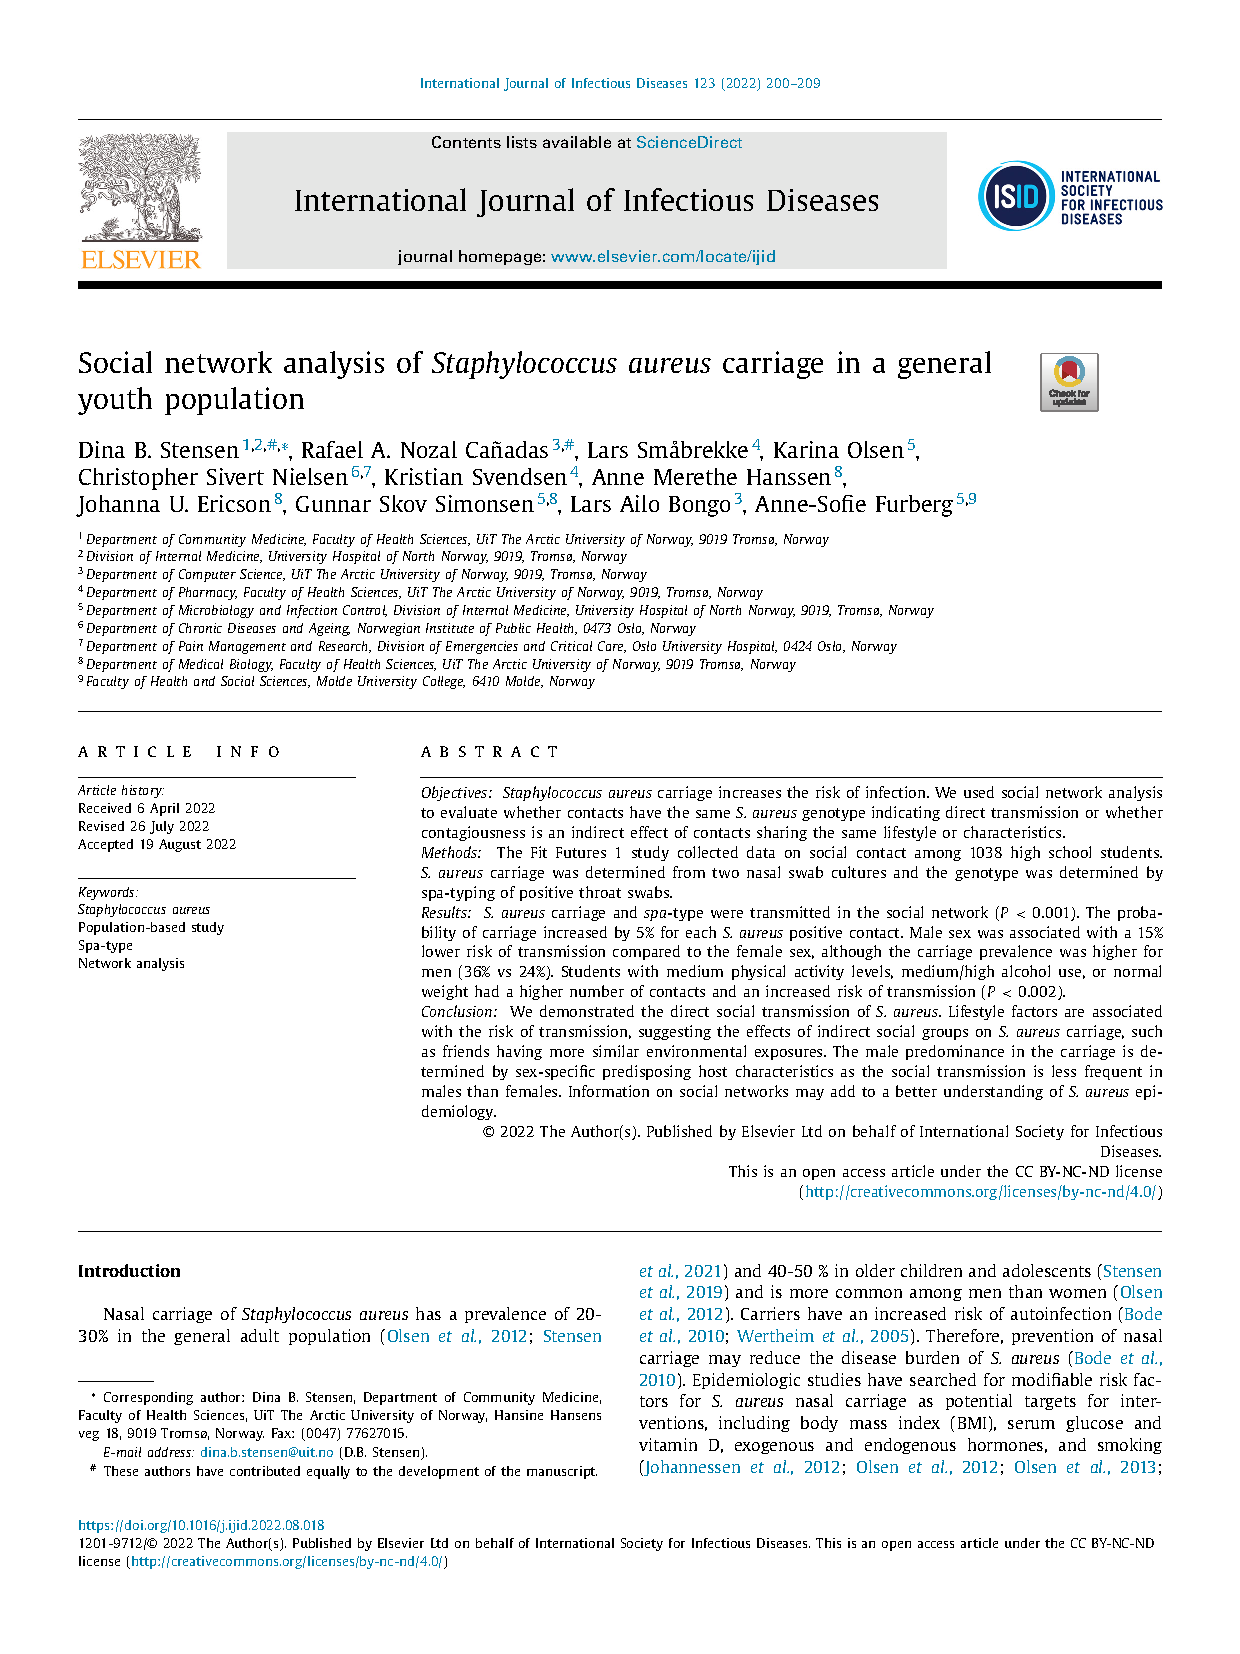
\includepdf[pages=-, width = \textwidth]{Annex/Papers/staph_paper}

\label{annex:PaperASup}
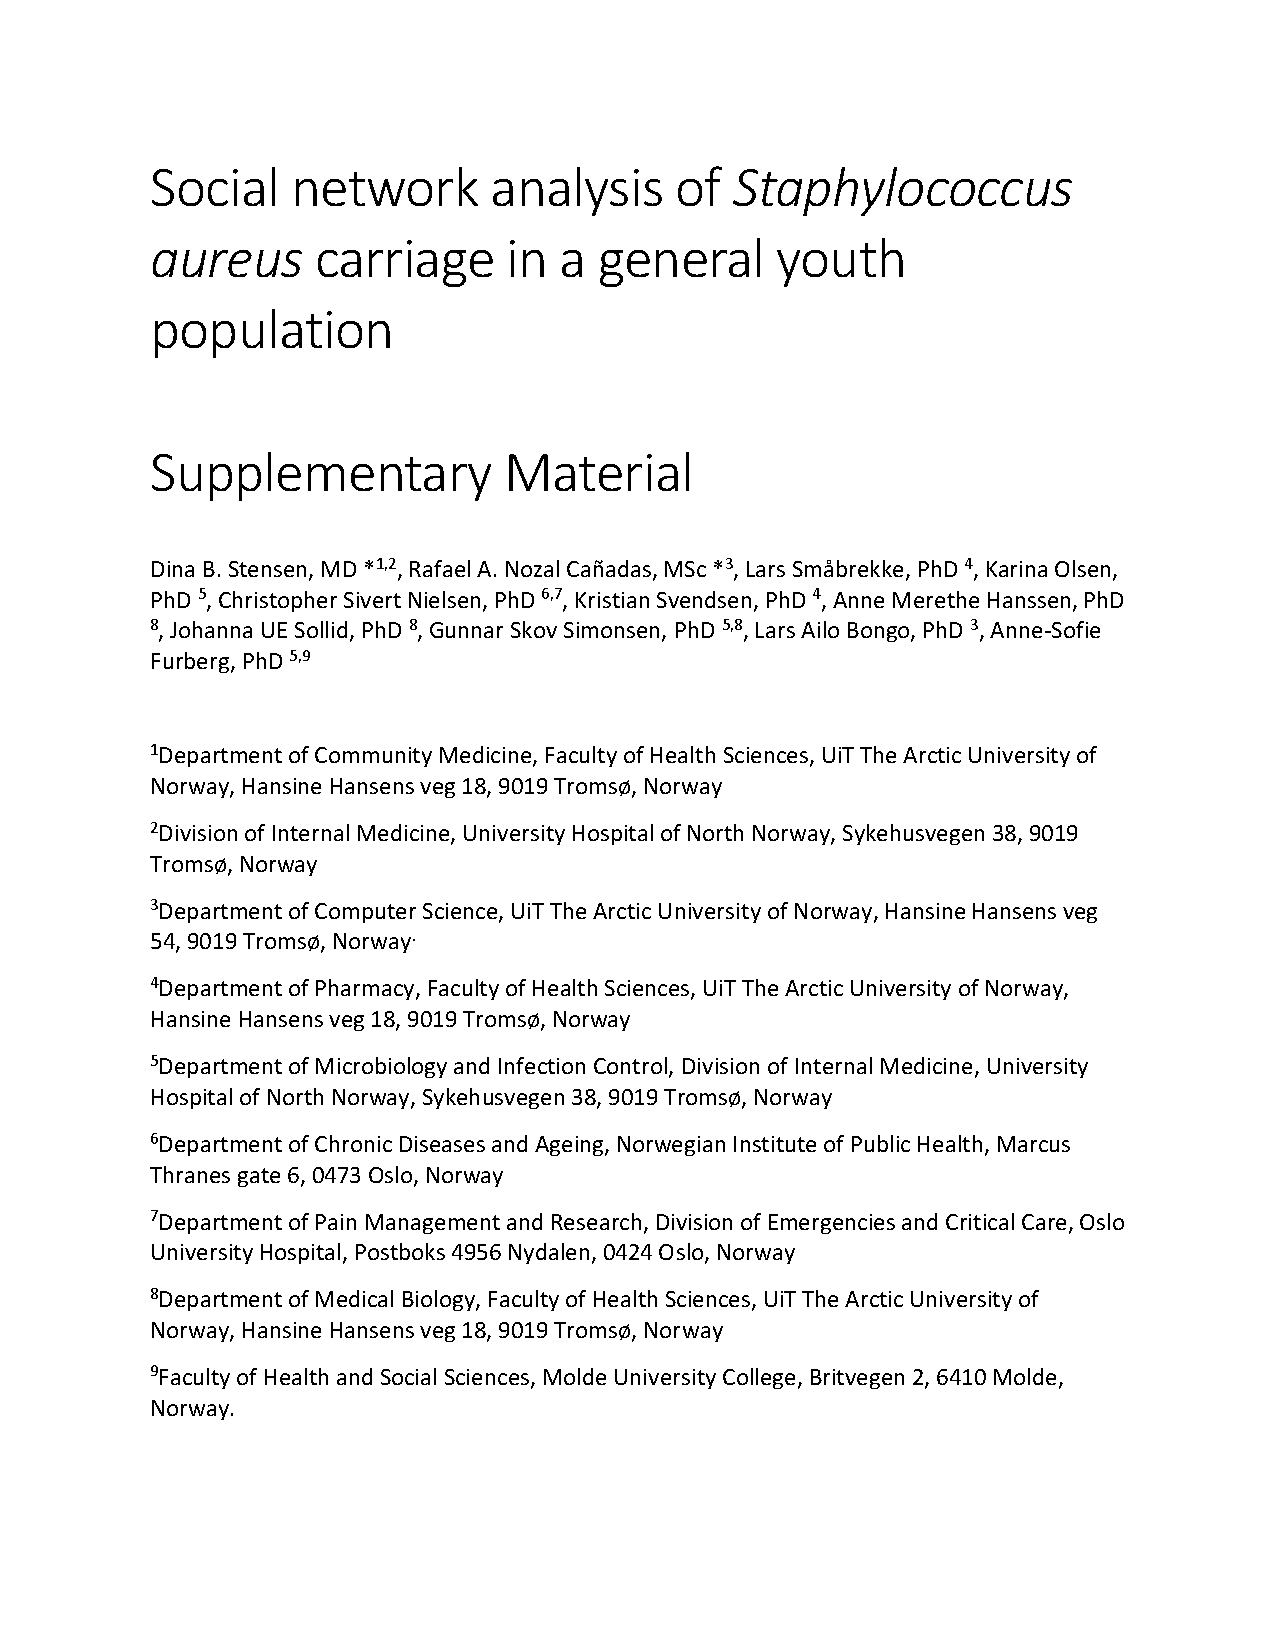
\includepdf[pages=-, width=\textwidth]{Annex/Papers/A_staph_supplementary}

% ---- B ----
\section{Paper B}
\label{annex:PaperB}
\includepdf[pages=-, width=\textwidth ]{Annex/Papers/Vitamin_D-Arxiv_V1}

%\label{annex:PaperC}
%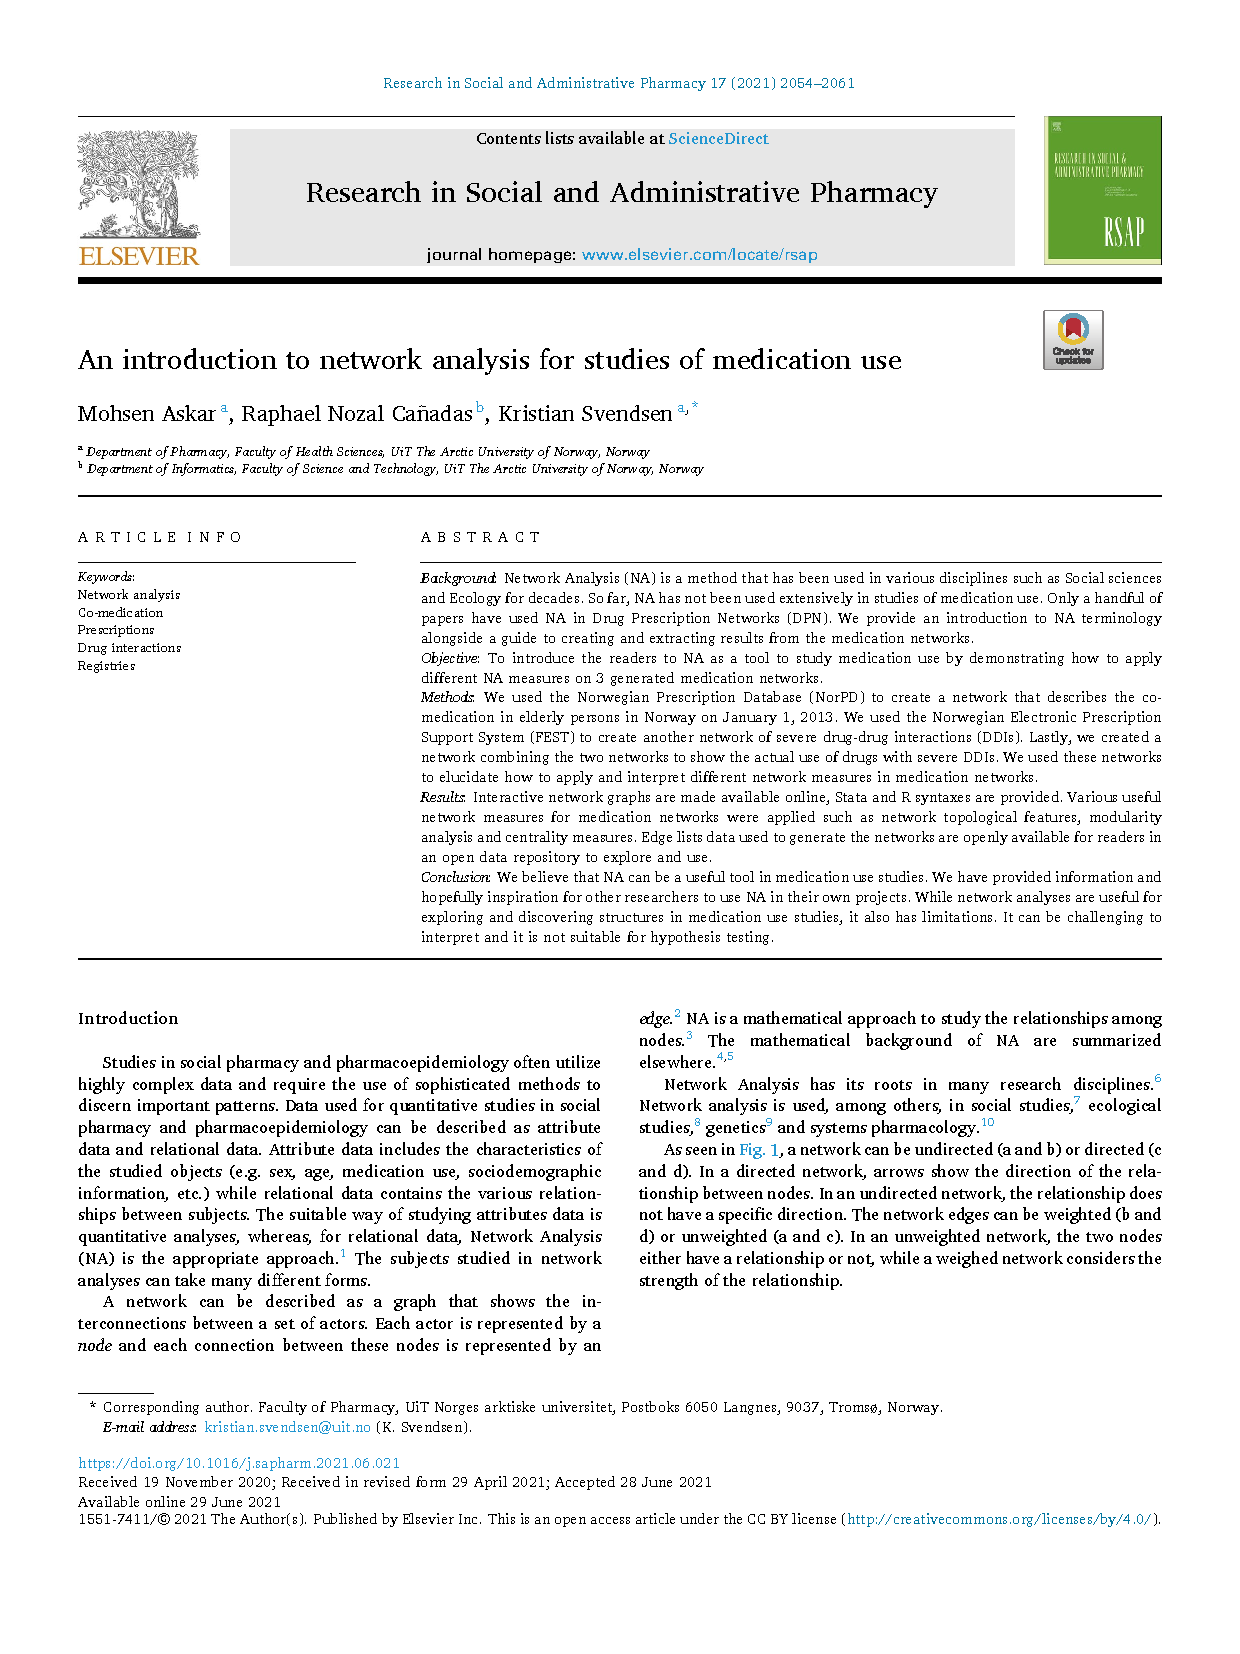
\includepdf[pages=-, nup=1x1, scale = 0.85 ]{Annex/Papers/network_paper}

\section{Paper C}

% ---- C ----
\label{annex:PaperC}
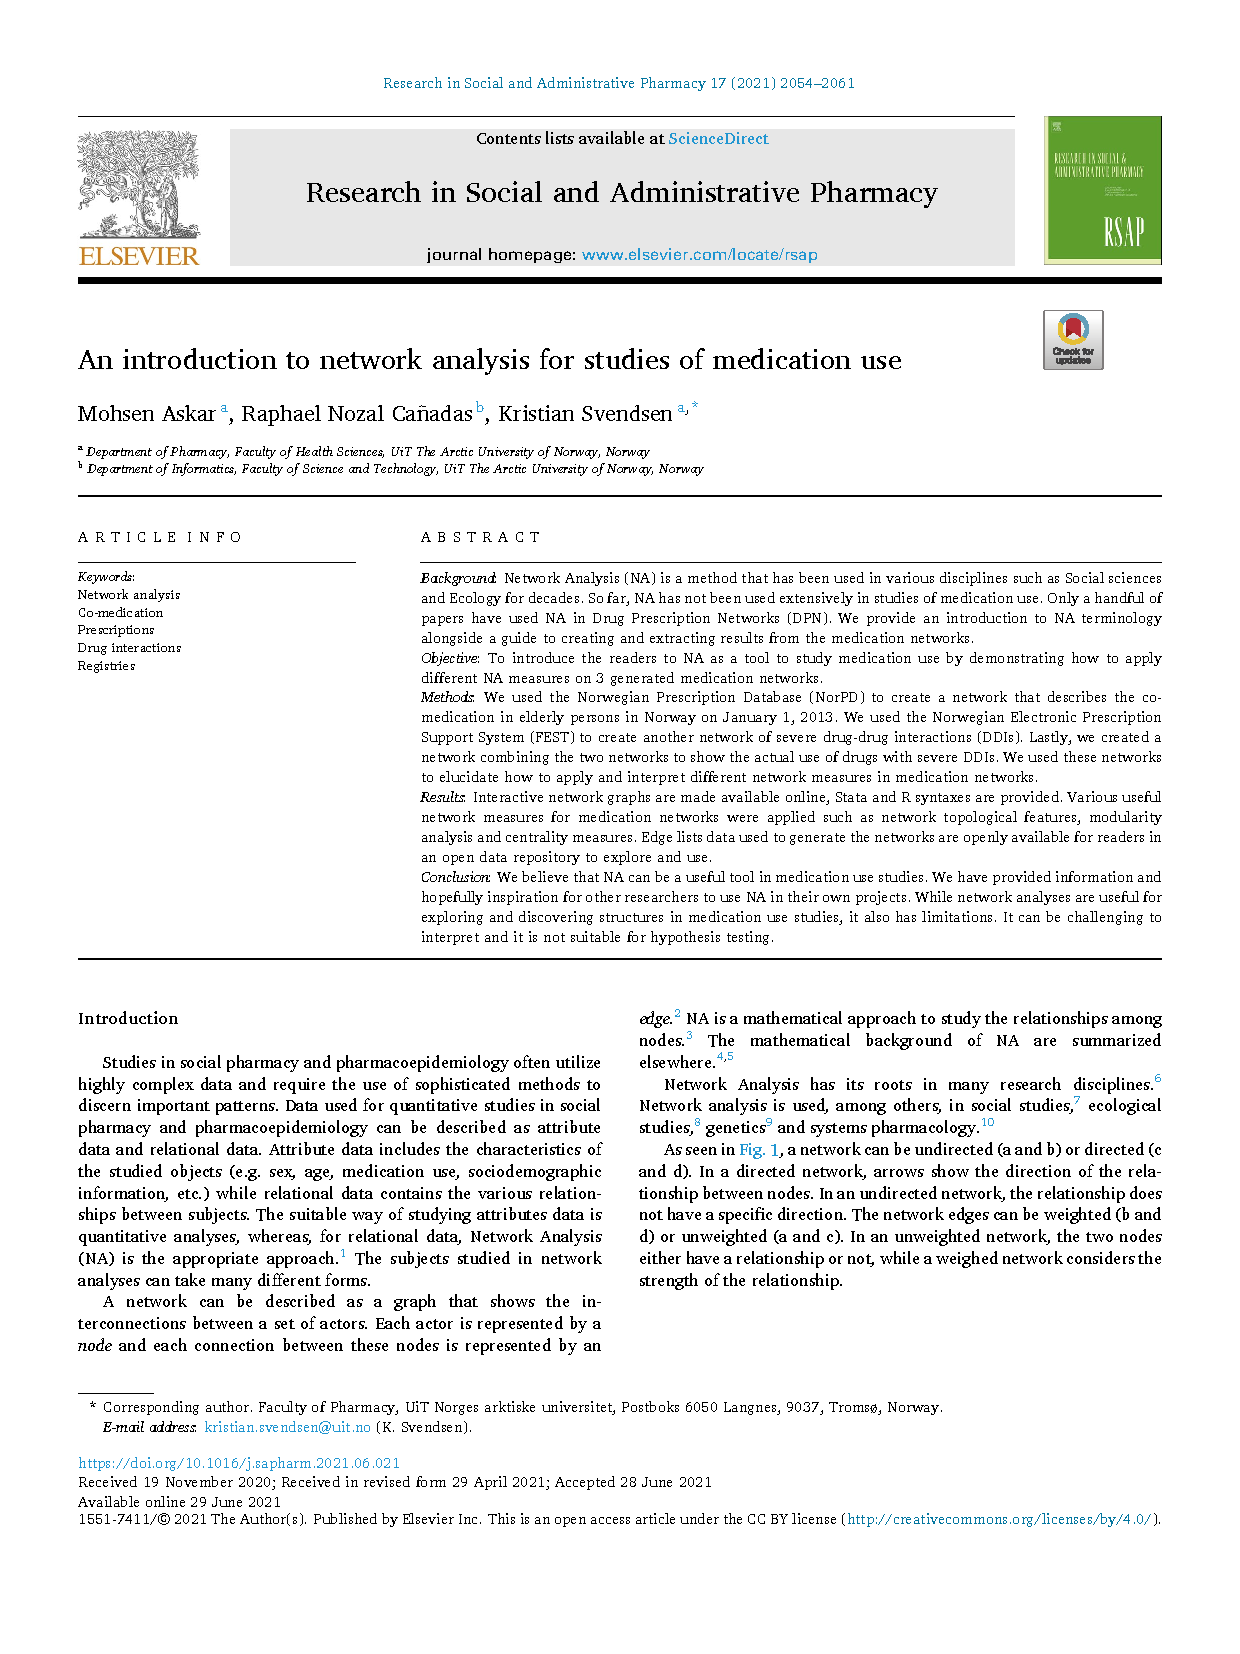
\includepdf[pages=-, nup=1x1, scale = 0.95, width=\textwidth ]{Annex/Papers/network_paper}

% Github structure here

% Necessary screenshots

% Extra results
%*****************************************
\chapter{Preliminary Results}
\label{chapter:chapter results}
%*****************************************

In this chapter, we explore the latest findings and ongoing research that form a crucial part of my PhD work. These results bear significant relevance to this thesis and enrich our understanding of the research domain, although still in progress and yet to be formally published. By including these preliminary findings, we aim to provide a comprehensive and up-to-date exploration of the topic. It is important to note that these findings are presented as drafts and are subject to further refinement and validation before publication.

\section{Result I}

\textbf{Social network influences on obesity in a general youth population.}

In recent years studies have evaluated the effect of peer pressure on obesity, via close friend networks in adults \cite{Christakis2007, Oliveira2013, Powell2015} and adolescents \cite{Fowler2008}, or direct advertising of junk food \cite{Dixon2007} or healthy habits \cite{Turner2017}. These studies have shown that people’s health, including obesity, tends to become similar to those in their social network. We would like to check if these results also apply to our student population and how these evolve over time.

In these results (tables \ref{table:resultOneBigTable}, \ref{table:resultSimulations}  figures \ref{figure:Results1general}, \ref{figure:Results1evolutionBMI}), first, we showed the social dynamics with respect to BMI (table \ref{table:resultOneBigTable}). We show that this population behaves similarly to other student populations \cite{DIXON20071311, Deoke2012, Lasserre2007}, and there is a bias in forming friendships with respect to BMI. "Overweight" and "Obese" students tend to form connections with each other, while at the same "Obese" students have lower connectivity are more isolated in the network, and seem to have a negative bias towards "Healthy" students. On the other hand, "Healthy" form connections mostly among themselves, with a negative bias toward both "Overweight" and "Obese". Using the same simulation technique as in Paper A (section \ref{sec:MetodologySimulations}), we also show a bias toward obesity spread in all networks (table \ref{table:resultSimulations}), being stronger in the "Sports" network, and weaker in the "School" network.

    \begin{table}

    \caption{ Bias with respect to the total number of relationships between each BMI category. The top column shows the absolute and relative frequencies of the population (n = 1034). People with unknown BMI are excluded from the analysis (n = 4). Each combination of categories represents people who nominate a friend (rows) and people who are nominated (columns). Each cell is divided into three parts, the left-most is the total number of relationships in this combination, the center one is the expected number of relationships (only given if a bias was found), the right part contains an arrow indicating over (up \textcolor{Green}{\textbf{↑}}) or underrepresented (down \textcolor{Red}{\textbf{↓}}) using a two-sided binomial test with at least p-value < 0.1.  The table Xi² test is < $10^{-10}$. In the bottom and to the left, we have the marginal absolute and relative frequencies for each combination. }

    \centering

    \label{table:resultOneBigTable}

    \renewcommand{\arraystretch}{1.2}

    \scalebox{0.70}{

    \begin{tabular}{|l|rrr:rrc:rrc:rrc|rr|} 
    
    \hline
    
    \begin{tabular}[c]{@{}l@{}}\end{tabular} &
    \multicolumn{3}{c}{{\cellcolor[rgb]{0.937,0.937,0.937}}
    
    \begin{tabular}[c]{@{}>{\cellcolor[rgb]{0.937,0.937,0.937}}c@{}}Underweight \\ n = 110 , f = .106\end{tabular}} &
    \multicolumn{3}{c}{{\cellcolor[rgb]{0.937,0.937,0.937}}
    
    \begin{tabular}[c]{@{}>{\cellcolor[rgb]{0.937,0.937,0.937}}c@{}}Healthy \\ n = 710 , f = .684\end{tabular}} &
    \multicolumn{3}{c}{{\cellcolor[rgb]{0.937,0.937,0.937}}
    
    \begin{tabular}[c]{@{}>{\cellcolor[rgb]{0.937,0.937,0.937}}c@{}}Overweight \\ n = 147 , f = .142\end{tabular}} &
    \multicolumn{3}{c|}{{\cellcolor[rgb]{0.937,0.937,0.937}}
    
    \begin{tabular}[c]{@{}>{\cellcolor[rgb]{0.937,0.937,0.937}}c@{}}Obese \\ n = 67 , f = .064\end{tabular}} &
    
    \multicolumn{1}{c}{{\cellcolor[rgb]{0.886,0.937,0.851}}Total} & \multicolumn{1}{c|}{{\cellcolor[rgb]{0.886,0.937,0.851}}Freq}  \\ 
    
    \hline
    
    {\cellcolor[rgb]{0.937,0.937,0.937}}Underweight & 47  &  & & 285  & & \multicolumn{1}{r:}{} & 48  & & \multicolumn{1}{r:}{} & 24 & & \multicolumn{1}{r|}{} & 404 & 10.8\% \\
    
    {\cellcolor[rgb]{0.937,0.937,0.937}}Healthy                                             & 282 &  &                                                                                                                                                               & 1870 & (1822) & \textbf{\textcolor[rgb]{0,0.502,0}{↑}}                                                                                                                      & 345 & (367) & \textbf{\textcolor{red}{↓}}                                                                                                                             & 90 & (122) & \textcolor{red}{↓}                                                                                                                                  & 2587                                                          & 69.1\%                                                         \\
{\cellcolor[rgb]{0.937,0.937,0.937}}Overweight                                          & 46  &  &                                                                                                                                                               & 347  &        &                                                                                                                                                    & 97  & (74)  & \textbf{\textcolor[rgb]{0,0.502,0}{↑}}                                                                                                                  & 34 & (24)  & \textcolor[rgb]{0,0.502,0}{\textbf{↑}}                                                                                                                       & 524                                                           & 14.0\%                                                         \\
{\cellcolor[rgb]{0.937,0.937,0.937}}Obese                                               & 22  &  &                                                                                                                                                               & 135  & (160)  & \textcolor{red}{\textbf{↓}}                                                                                                                                 & 42  & (32)  & \textcolor[rgb]{0,0.502,0}{\textbf{↑}}                                                                                                                  & 29 & (10)  & \textbf{\textcolor[rgb]{0,0.502,0}{↑}}                                                                                                                       & 228                                                           & 6.1\%                                                          \\ 
\hline
{\cellcolor[rgb]{0.886,0.937,0.851}}Total                                               & \multicolumn{3}{c}{397}                                                                                                                                                & \multicolumn{3}{c}{2637}                                                                                                                                           & \multicolumn{3}{c}{532}                                                                                                                                               & \multicolumn{3}{c|}{177}                                                                                                                                         & \multicolumn{1}{l}{3743}                                      & \multicolumn{1}{l|}{}                                          \\
{\cellcolor[rgb]{0.886,0.937,0.851}}Frequency                                           & \multicolumn{3}{c}{10.6\%}                                                                                                                                             & \multicolumn{3}{c}{70.5\%}                                                                                                                                         & \multicolumn{3}{c}{14.2\%}                                                                                                                                            & \multicolumn{3}{c|}{4.7\%}                                                                                                                                       & \multicolumn{1}{l}{}                                          & \multicolumn{1}{l|}{100\%}                                     \\
\hline
\end{tabular}

}



\end{table}



\begin{table}[H]

\caption{Results of the spread of BMI across all networks simulations. The first column is the name of the network. Second is how many relationships are in that network. The third column is how many of those relationships share the same BMI category. The next 7 columns are the details of the simulation results, with the important one being the ”Average“ and ”SD (Standard Deviation)”, which shows how many same-to-same relationships in average we had in the 1000 simulations, using a network with the same topology but randomizing the BMI according to the BMI probability density data of the original network. The last column is the p-value, rounded to 3 decimals, which shows if there is a significant difference between the averaged same-to-same simulated relationship and the real same-to-same relationships.}

\centering

\label{table:resultSimulations}

\renewcommand{\arraystretch}{1.2}
\scalebox{0.70}{

\begin{tabular}{l|rr|rrrrrrr|r}
\cline{2-10}
                                                      & \multicolumn{2}{c|}{\cellcolor[HTML]{F7CAAC}Real networks}                                                                         & \multicolumn{7}{c|}{\cellcolor[HTML]{FFE599}Simulated 1000 networks}                                                                                                                                                                                                                                                                                             & \multicolumn{1}{c}{}                                 \\ \hline
\rowcolor[HTML]{FFF2CC} 
\multicolumn{1}{|c|}{\cellcolor[HTML]{D9E2F3}Network} & \multicolumn{1}{c}{\cellcolor[HTML]{FBE4D5}Total Relationships} & \multicolumn{1}{c|}{\cellcolor[HTML]{FBE4D5}Equal Relationships} & \multicolumn{1}{c}{\cellcolor[HTML]{FFF2CC}MIN} & \multicolumn{1}{c}{\cellcolor[HTML]{FFF2CC}Q1} & \multicolumn{1}{c}{\cellcolor[HTML]{FFF2CC}Median} & \multicolumn{1}{c}{\cellcolor[HTML]{FFF2CC}Average} & \multicolumn{1}{c}{\cellcolor[HTML]{FFF2CC}Q3} & \multicolumn{1}{c}{\cellcolor[HTML]{FFF2CC}MAX} & \multicolumn{1}{c|}{\cellcolor[HTML]{FFF2CC}SD} & \multicolumn{1}{c|}{\cellcolor[HTML]{E2EFD9}P-value} \\ \hline
\multicolumn{1}{|l|}{Overall}                         & {\color[HTML]{9B9B9B} 3767}                                     & 2043                                                             & {\color[HTML]{9B9B9B} 1761}                     & {\color[HTML]{9B9B9B} 1853}                    & {\color[HTML]{9B9B9B} 1893}                        & 1894.1                                              & {\color[HTML]{9B9B9B} 1934}                    & {\color[HTML]{9B9B9B} 2077}                     & {\color[HTML]{9B9B9B} 59.5}                     & \multicolumn{1}{r|}{0.006}                           \\
\multicolumn{1}{|l|}{Physical}                        & {\color[HTML]{9B9B9B} 2823}                                     & 1584                                                             & {\color[HTML]{9B9B9B} 1233}                     & {\color[HTML]{9B9B9B} 1368}                    & {\color[HTML]{9B9B9B} 1402}                        & 1406.1                                              & {\color[HTML]{9B9B9B} 1445}                    & {\color[HTML]{9B9B9B} 1561}                     & {\color[HTML]{9B9B9B} 59.6}                     & \multicolumn{1}{r|}{0.001}                           \\
\multicolumn{1}{|l|}{School}                          & {\color[HTML]{9B9B9B} 2979}                                     & 1590                                                             & {\color[HTML]{9B9B9B} 1337}                     & {\color[HTML]{9B9B9B} 1459}                    & {\color[HTML]{9B9B9B} 1490}                        & 1493.7                                              & {\color[HTML]{9B9B9B} 1536}                    & {\color[HTML]{9B9B9B} 1647}                     & {\color[HTML]{9B9B9B} 59.9}                     & \multicolumn{1}{r|}{0.054}                           \\
\multicolumn{1}{|l|}{Sports}                          & {\color[HTML]{9B9B9B} 598}                                      & 415                                                              & {\color[HTML]{9B9B9B} 257}                      & {\color[HTML]{9B9B9B} 289}                     & {\color[HTML]{9B9B9B} 303}                         & 301.9                                               & {\color[HTML]{9B9B9B} 314}                     & {\color[HTML]{9B9B9B} 355}                      & {\color[HTML]{9B9B9B} 19.1}                     & \multicolumn{1}{r|}{\textless{}0.0001}               \\
\multicolumn{1}{|l|}{Home}                            & {\color[HTML]{9B9B9B} 1247}                                     & 722                                                              & {\color[HTML]{9B9B9B} 563}                      & {\color[HTML]{9B9B9B} 603}                     & {\color[HTML]{9B9B9B} 621}                         & 624.3                                               & {\color[HTML]{9B9B9B} 645}                     & {\color[HTML]{9B9B9B} 709}                      & {\color[HTML]{9B9B9B} 29.9}                     & \multicolumn{1}{r|}{0.001}                           \\
\multicolumn{1}{|l|}{Other}                           & {\color[HTML]{9B9B9B} 1095}                                     & 612                                                              & {\color[HTML]{9B9B9B} 488}                      & {\color[HTML]{9B9B9B} 532}                     & {\color[HTML]{9B9B9B} 552}                         & 552.7                                               & {\color[HTML]{9B9B9B} 575}                     & {\color[HTML]{9B9B9B} 623}                      & {\color[HTML]{9B9B9B} 28.8}                     & \multicolumn{1}{r|}{0.020}                           \\ \hline
\end{tabular}

}



\end{table}

We checked for the general evolution of BMI over time (figure \ref{figure:Results1general}). We observed that roughly half of the “Underweights” go into the “Healthy” group while almost none of the “Healthy” descent into the “Underweights”. However, a similar trend is seen with a big group of “Healthy” going into “Overweight” without barely “Overweight” descending into “Healthy”. There is also another group going from “Overweight” to “Obese”; this group is larger than the group descending to “Healthy”. Both “Underweight” and “Healthy” groups decrease in size while both “Overweight” and “Obese” increase. Some from the “Obese” group descent into the “Overweight” group, but not enough to compensate for those new students entering the group. The average BMI (kg/m2) in FF1 was 22.57 ± 4.23, and in FF2 was 23.32 ± 4.25. For men, in FF1 was 22.51 ± 4.22 and 23.55 ± 4.19 in FF2. For women was 22.62 ± 4.24 in FF1 and 23.12 ± 4.30 in FF2.

    \begin{figure}[ht]
        \centering
            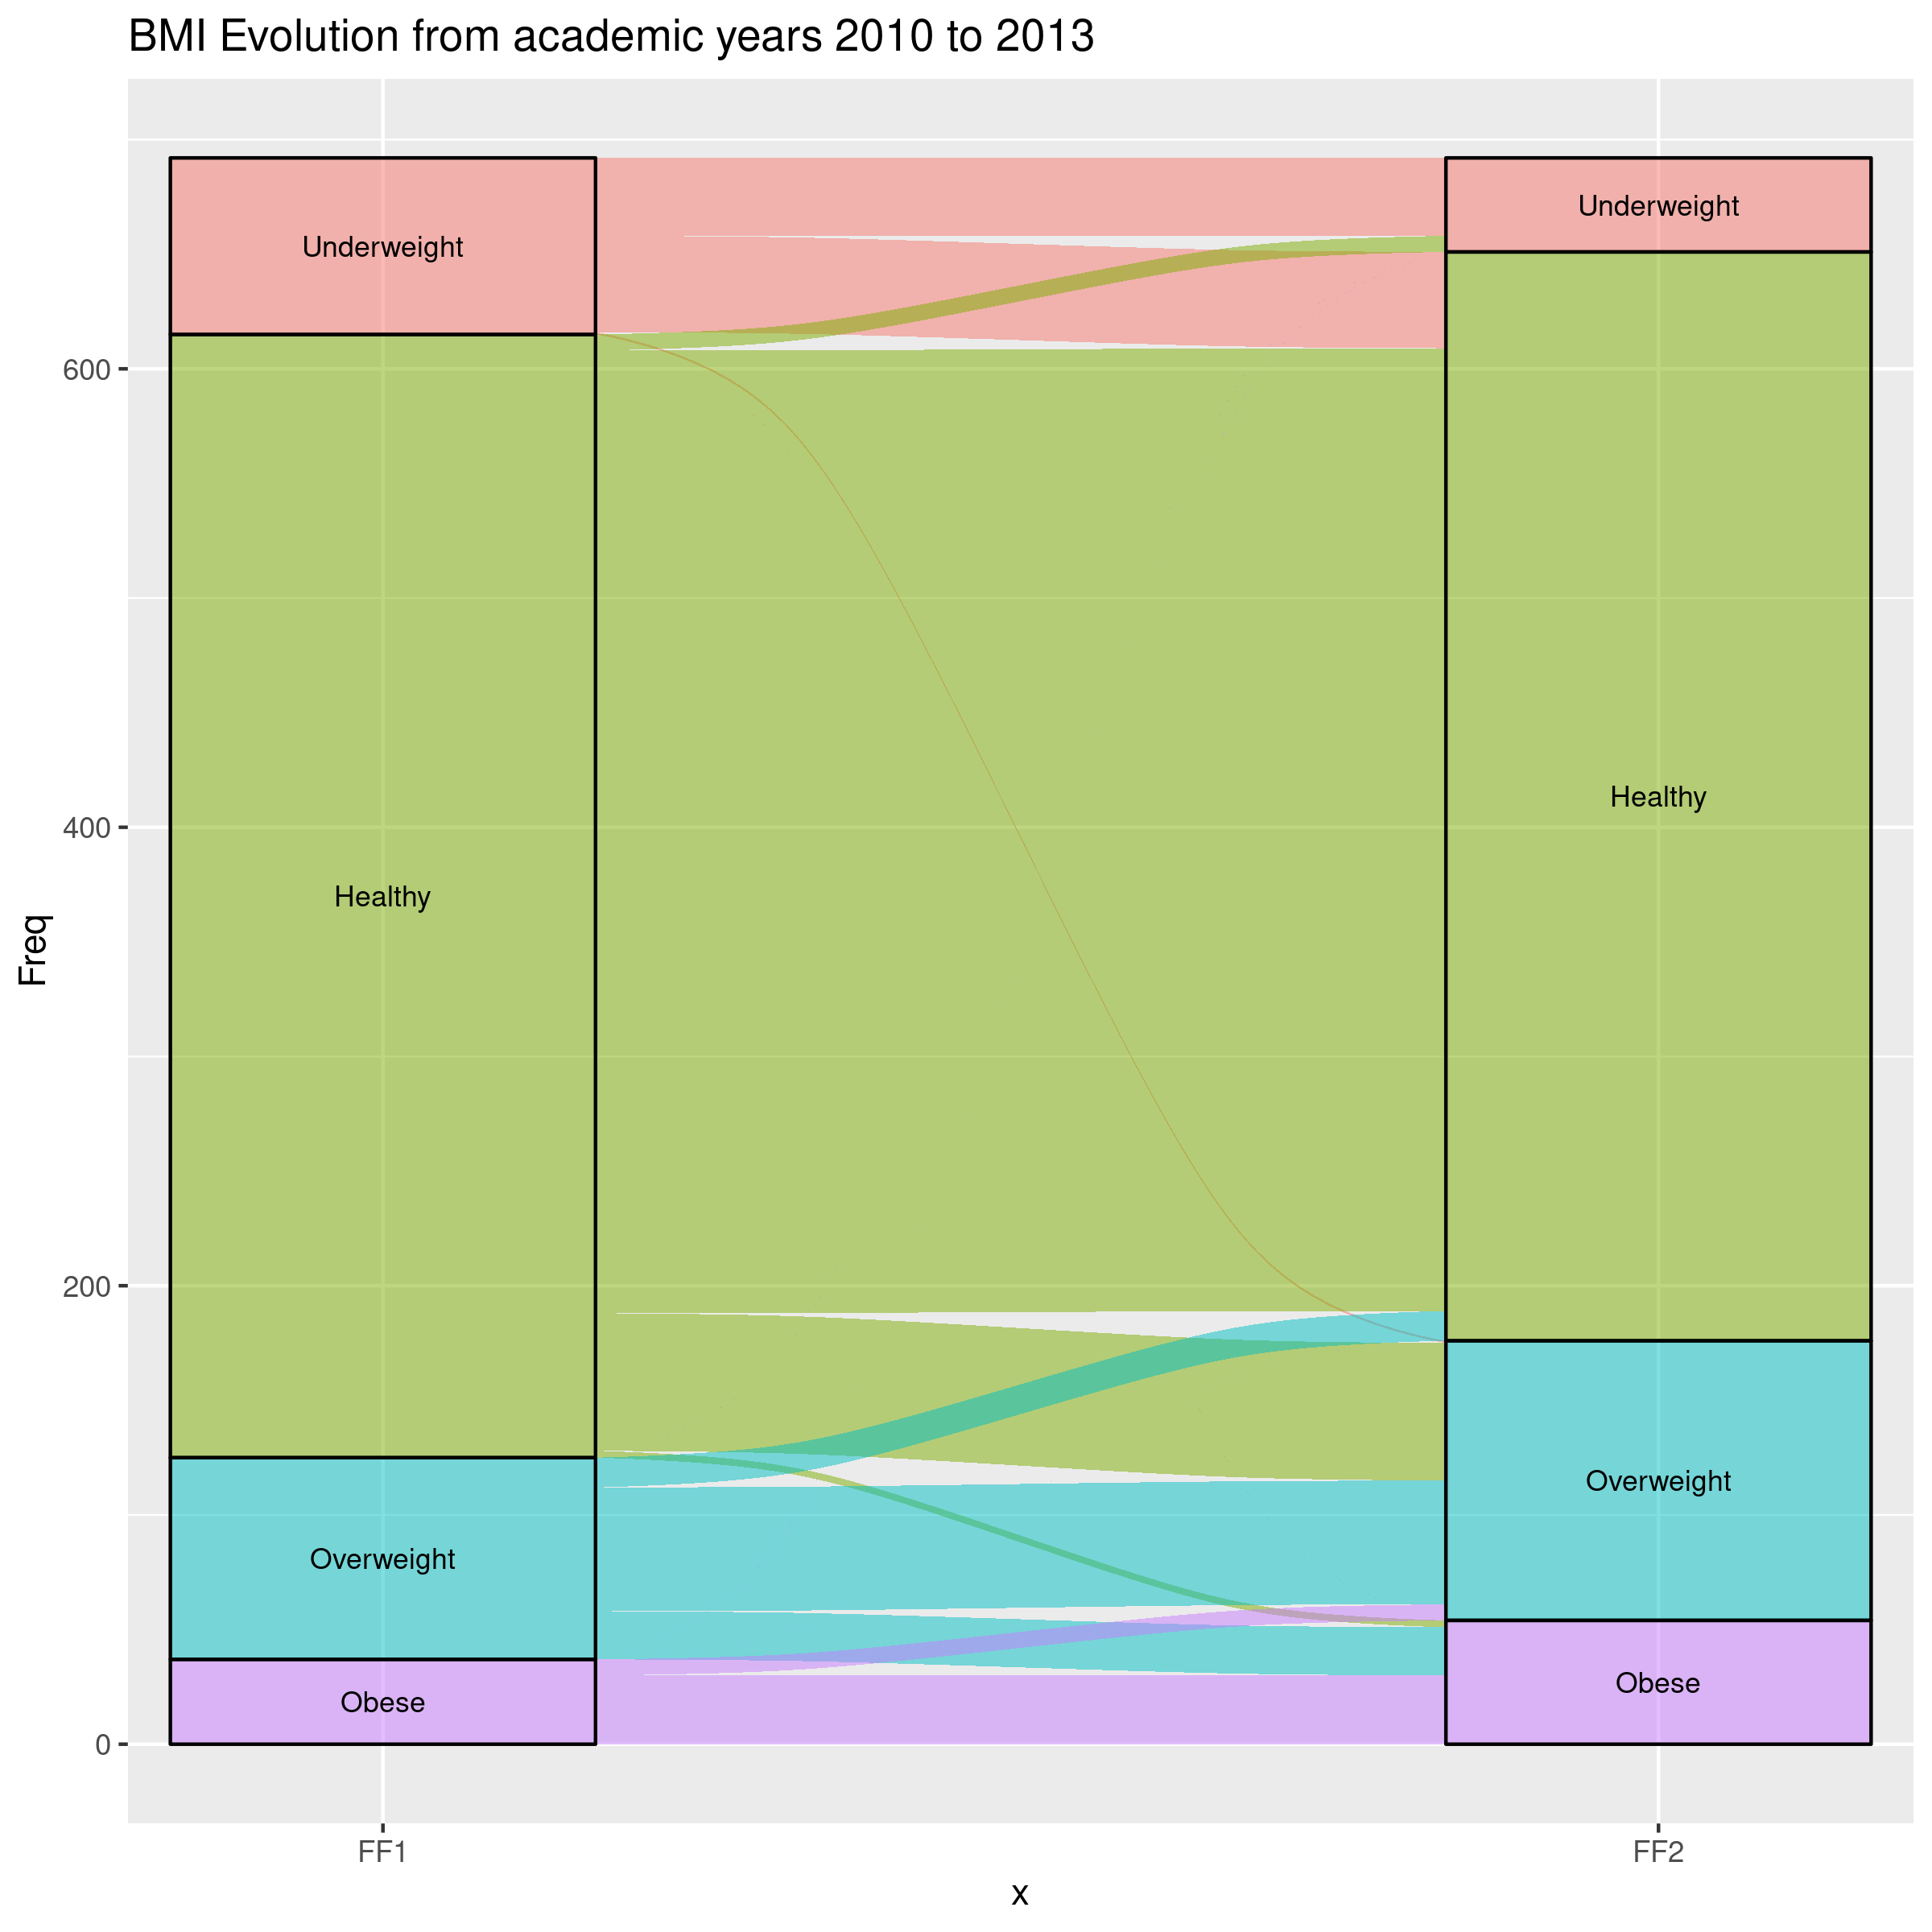
\includegraphics[width=0.75\linewidth]{figures/Results/ResultOne/generalEvolution.png } 
        \caption{An overview of the evolution of BMI from Fit Futures 1 (2010-2011) to Fit Futures 2 (2012-2013) for every student with valid BMI data in both studies (n = 692). On the left column, we have the FF1 BMI categories. In the right column, we have the FF2 categories two years later. The threads from left to right indicate the evolution of each person with respect to the BMI category.}
        \label{figure:Results1general}
    \end{figure}

We also tested if the number of high BMI friends is related to the BMI value in FF2 (figure \ref{figure:Results1evolutionBMI}). On average, the “Healthy” and “Underweight” groups tend to go down in FF2, the greater the number of friends with BMI>25 they had during FF1. We only see a sharp decrease in “Overweight” for the number of friends equal to 5, but they go into the “Obese” category instead which is a sharp increase in this group. Using logistic regression we estimated an 8.5\% increase in the risk of high BMI with respect to each additional "Overweight" or "Obese" friend. We also show that as the number of friends in FF1 with BMI > 25 increases, there is a higher probability of not landing in the "Healthy" group in FF2, and is also likely that the student will land in "Overweight" or "Obese" instead.

    \begin{figure}[ht]
        \centering
            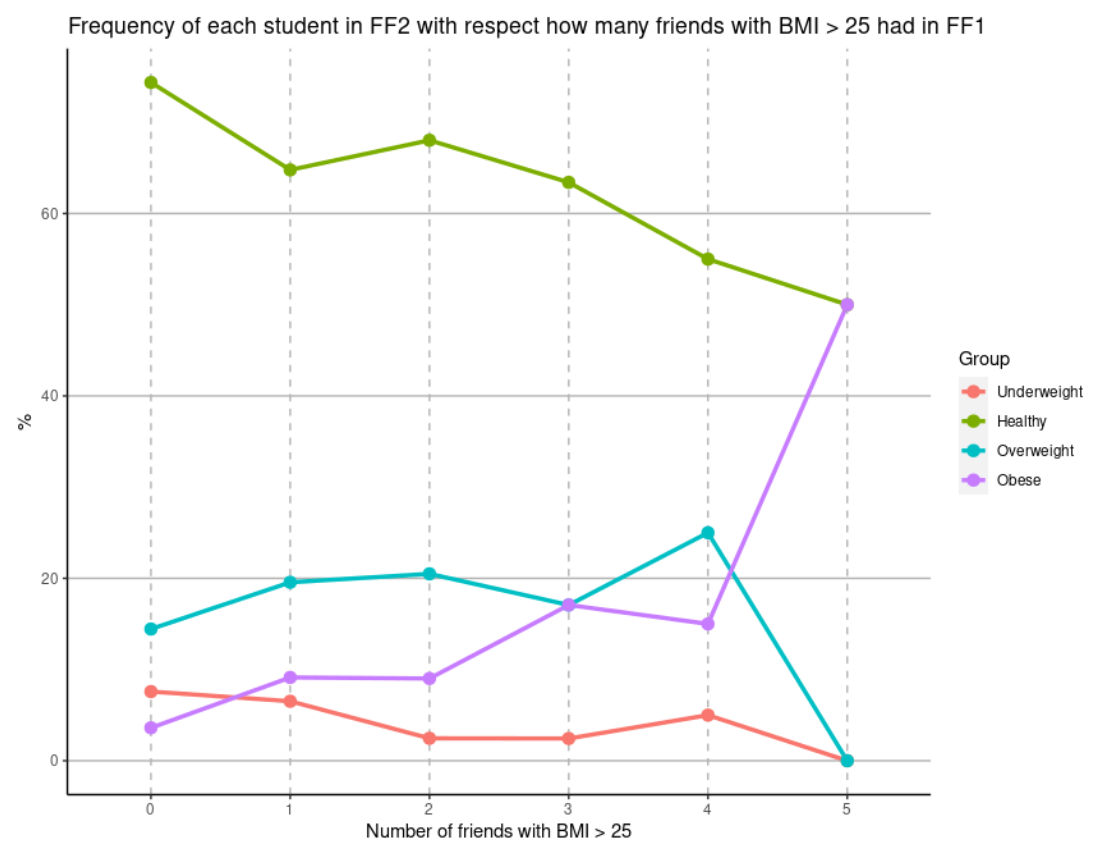
\includegraphics[width=0.75\linewidth]{figures/Results/ResultOne/bmiInfluence.png } 
        \caption{ The influence of friends from FF1 have with respect to FF2 BMI. The X-axis is the number of friends in FF1 with BMI>25 kg/m2 The Y-axis is the relative number of students belonging to each BMI category in FF2.}
        \label{figure:Results1evolutionBMI}
    \end{figure}

Overall, these results seem to indicate that friendship is stagnated and students tend to keep within the same BMI group. And more importantly, an individual with "Healthy" friends has a better chance of being "Healthy" in the future, and an individual with "Overweight" or "Obese" friends has also a better chance of being "Overweight" or "Obese" in the future as well.


\section{Result II}

\textbf{Social network influences on inflammatory response in a general youth population.}

Chronic inflammation is a health concern with evidence suggesting that it contributes to the pathogenesis of numerous diseases, including cancer, cardiovascular disease, diabetes, and neurodegenerative disorders. Obesity has been shown to be correlated from childhood to adulthood \cite{Woo2019}, while also being responsible for a range of adverse health conditions. Inflammation is shown to vary as a function of social isolation; in particular social behavior and the inflammatory process seem to be regulating one another \cite{Zhang2015, Karczewski2018, Safaei2021, Eisenberger2016, Bang2019, Henriquez2022, Koyama2021}. Obesity is also an underlying condition in both chronic inflammation and metabolic diseases \cite{Lee2013, Karczewski2018, Dhurandhar2014CounteringTE}. In this explorative study, we investigate how the three concepts of inflammation in the form of a 92 proteomic assay, obesity in the form of anthropometric variables, and social interaction in the form of our network of friends, are related to one another. In particular, we look if there is a similarity of inflammation among social contacts. We found some results in the data that suggest that inflammatory markers are common among friends of the same sex and the same high school suggesting that social influence has an underlying link.

To evaluate if there is a correlation between each person and his/her friends’ biomarker levels, we tried regression models (linear, quadratic, logarithmic, or exponential) using each person’s friends’ average biomarker level as the independent variable, and the person’s biomarker levels as the dependent variable. Without any stratification by sex or by high school, we found no statistically relevant results for any biomarker. We found no correlation for sex stratification using all high schools. But biomarker levels are influenced by sex and social influence is driven by high school. If we stratify by these two variables; we found a total of 50 biomarkers for men and 46 for women that are significant with respect to some high schools (tables \ref{table:Result1MalesRegression} and \ref{table:Result1FemalesRegression}). This suggests that some biomarker levels are influenced by the student’s social network, and in particular by high school, which has a relevant homophily coefficient (87.85\% p-value <0.0001). Furthermore, high schools where blood samples were extracted later during the academic year (March / April 2011) show a higher amount of biomarkers correlation in contrast with other schools (October 2010 to March 2011). For High School 5, we found 13 markers for men, 11 for women; for High School 6, 23 for men, 17 for women; and for the rest of high schools combined 14 for men, 18 for women.

\begin{table}[ht]

\caption{ Overview of all biomarkers with respect to each high school (n=8) for men. All biomarkers with either R2 < 0.2 and p-value > 0.05, are hidden from the tables. P-values are expressed in GP Prism 5.04/d format.}

\centering

\renewcommand{\arraystretch}{1.2}

\scalebox{0.70}{
\begin{tabular}{clll}
\rowcolor[HTML]{01C0DB} 
{\color[HTML]{FFFFFF} \textbf{Highschool}} & {\color[HTML]{FFFFFF} \textbf{Protein}}                                               & {\color[HTML]{FFFFFF} \textbf{R2}} & {\color[HTML]{FFFFFF} \textbf{P-value}} \\ \hline
                                           & C-X-C motif chemokine 9                                                               & 0.26                               & *                                       \\
                                           & Eotaxin                                                                               & 0.33                               & **                                      \\
                                           & Interleukin-10                                                                        & 0.55                               & ****                                    \\
                                           & Interleukin-10 receptor subunit alpha                                                 & 0.25                               & **                                      \\
                                           & \cellcolor[HTML]{EFEFEF}Interleukin-13                                                & \cellcolor[HTML]{EFEFEF}0.66       & \cellcolor[HTML]{EFEFEF}****            \\
                                           & \cellcolor[HTML]{EFEFEF}Interleukin-33                                                & \cellcolor[HTML]{EFEFEF}0.27       & \cellcolor[HTML]{EFEFEF}**              \\
                                           & \cellcolor[HTML]{EFEFEF}Interleukin-6                                                 & \cellcolor[HTML]{EFEFEF}0.28       & \cellcolor[HTML]{EFEFEF}*               \\
                                           & \cellcolor[HTML]{EFEFEF}Interleukin-8                                                 & \cellcolor[HTML]{EFEFEF}0.24       & \cellcolor[HTML]{EFEFEF}**              \\
                                           & Macrophage colony-stimulating factor 1                                                & 0.49                               & ****                                    \\
\multirow{-10}{*}{H2}                      & Oncostatin-M                                                                          & 0.26                               & *                                       \\ \hline
                                           & Cystatin D                                                                            & 0.21                               & **                                      \\
\multirow{-2}{*}{H3}                       & STAM-binding protein                                                                  & 0.23                               & ***                                     \\ \hline
H4                                         & \cellcolor[HTML]{EFEFEF}Leukemia inhibitory factor receptor                           & \cellcolor[HTML]{EFEFEF}0.27       & \cellcolor[HTML]{EFEFEF}***             \\ \hline
                                           & \cellcolor[HTML]{EFEFEF}Adenosine Deaminase                                           & \cellcolor[HTML]{EFEFEF}0.44       & \cellcolor[HTML]{EFEFEF}****            \\
                                           & \cellcolor[HTML]{EFEFEF}Beta-nerve growth factor                                      & \cellcolor[HTML]{EFEFEF}0.22       & \cellcolor[HTML]{EFEFEF}**              \\
                                           & \cellcolor[HTML]{EFEFEF}C-C motif chemokine 28                                        & \cellcolor[HTML]{EFEFEF}0.28       & \cellcolor[HTML]{EFEFEF}**              \\
                                           & C-X-C motif chemokine 11                                                              & 0.21                               & *                                       \\
                                           & CD40L receptor                                                                        & 0.29                               & **                                      \\
                                           & CUB domain-containing protein 1                                                       & 0.23                               & *                                       \\
                                           & Fractalkine                                                                           & 0.48                               & ***                                     \\
                                           & \cellcolor[HTML]{EFEFEF}Interleukin-10                                                & \cellcolor[HTML]{EFEFEF}0.21       & \cellcolor[HTML]{EFEFEF}**              \\
                                           & \cellcolor[HTML]{EFEFEF}Interleukin-10 receptor subunit alpha                         & \cellcolor[HTML]{EFEFEF}0.34       & \cellcolor[HTML]{EFEFEF}**              \\
                                           & \cellcolor[HTML]{EFEFEF}Interleukin-17C                                               & \cellcolor[HTML]{EFEFEF}0.24       & \cellcolor[HTML]{EFEFEF}**              \\
                                           & \cellcolor[HTML]{EFEFEF}Macrophage colony-stimulating factor 1                        & \cellcolor[HTML]{EFEFEF}0.24       & \cellcolor[HTML]{EFEFEF}*               \\
                                           & Monocyte chemotactic protein 3                                                        & 0.21                               & **                                      \\
\multirow{-13}{*}{H5}                      & Tumor necrosis factor receptor superfamily member 9                                   & 0.4                                & ***                                     \\ \hline
                                           & Artemin                                                                               & 0.32                               & *                                       \\
                                           & Beta-nerve growth factor                                                              & 0.27                               & *                                       \\
                                           & \cellcolor[HTML]{EFEFEF}C-C motif chemokine 20                                        & \cellcolor[HTML]{EFEFEF}0.57       & \cellcolor[HTML]{EFEFEF}**              \\
                                           & \cellcolor[HTML]{EFEFEF}C-C motif chemokine 25                                        & \cellcolor[HTML]{EFEFEF}0.45       & \cellcolor[HTML]{EFEFEF}**              \\
                                           & \cellcolor[HTML]{EFEFEF}C-C motif chemokine 28                                        & \cellcolor[HTML]{EFEFEF}0.62       & \cellcolor[HTML]{EFEFEF}***             \\
                                           & \cellcolor[HTML]{EFEFEF}C-X-C motif chemokine 5                                       & \cellcolor[HTML]{EFEFEF}0.32       & \cellcolor[HTML]{EFEFEF}*               \\
                                           & C-X-C motif chemokine 6                                                               & 0.4                                & *                                       \\
                                           & Caspase-8                                                                             & 0.49                               & **                                      \\
                                           & CD40L receptor                                                                        & 0.72                               & ***                                     \\
                                           & CUB domain-containing protein 1                                                       & 0.63                               & ***                                     \\
                                           & \cellcolor[HTML]{EFEFEF}Delta and Notch-like epidermal growth factor-related receptor & \cellcolor[HTML]{EFEFEF}0.56       & \cellcolor[HTML]{EFEFEF}**              \\
                                           & \cellcolor[HTML]{EFEFEF}Fibroblast growth factor 23                                   & \cellcolor[HTML]{EFEFEF}0.49       & \cellcolor[HTML]{EFEFEF}**              \\
                                           & \cellcolor[HTML]{EFEFEF}Fractalkine                                                   & \cellcolor[HTML]{EFEFEF}0.41       & \cellcolor[HTML]{EFEFEF}*               \\
                                           & \cellcolor[HTML]{EFEFEF}Interferon gamma                                              & \cellcolor[HTML]{EFEFEF}0.4        & \cellcolor[HTML]{EFEFEF}*               \\
                                           & Interleukin-33                                                                        & 0.28                               & *                                       \\
                                           & Interleukin-8                                                                         & 0.57                               & **                                      \\
                                           & Leukemia inhibitory factor receptor                                                   & 0.49                               & **                                      \\
                                           & Neurotrophin-3                                                                        & 0.51                               & **                                      \\
                                           & \cellcolor[HTML]{EFEFEF}Oncostatin-M                                                  & \cellcolor[HTML]{EFEFEF}0.28       & \cellcolor[HTML]{EFEFEF}*               \\
                                           & \cellcolor[HTML]{EFEFEF}Osteoprotegerin                                               & \cellcolor[HTML]{EFEFEF}0.53       & \cellcolor[HTML]{EFEFEF}**              \\
                                           & \cellcolor[HTML]{EFEFEF}Programmed cell death 1 ligand 1                              & \cellcolor[HTML]{EFEFEF}0.47       & \cellcolor[HTML]{EFEFEF}**              \\
                                           & \cellcolor[HTML]{EFEFEF}TNF-related apoptosis-inducing ligand                         & \cellcolor[HTML]{EFEFEF}0.48       & \cellcolor[HTML]{EFEFEF}**              \\
\multirow{-23}{*}{H6}                      & Urokinase-type plasminogen activator                                                  & 0.65                               & ***                                    
\end{tabular}
}

\label{table:Result1MalesRegression}
\end{table}


\begin{table}[ht]
\caption{ Overview of all biomarkers with respect to each high school (n=8) for women. All biomarkers with either R2 < 0.2 and p-value > 0.05, are hidden from the tables. P-values are expressed in GP Prism 5.04/d format.}
\centering
\renewcommand{\arraystretch}{1.2}

\scalebox{0.70}{
\begin{tabular}{clll}
\rowcolor[HTML]{EF35AE} 
{\color[HTML]{FFFFFF} \textbf{Highschool}} & {\color[HTML]{FFFFFF} \textbf{Protein}}                                     & {\color[HTML]{FFFFFF} \textbf{R2}} & {\color[HTML]{FFFFFF} \textbf{P-value}} \\ \hline
                                           & Glial cell line-derived neurotrophic factor                                 & 0.26                               & ****                                    \\
\multirow{-2}{*}{H1}                       & Interferon gamma                                                            & 0.24                               & ***                                     \\ \hline
H2                                         & Tumor necrosis factor                                                       & 0.4                                & ****                                    \\ \hline
                                           & Fibroblast growth factor 19                                                 & 0.23                               & **                                      \\
                                           & \cellcolor[HTML]{EFEFEF}Interleukin-10 receptor subunit beta                & \cellcolor[HTML]{EFEFEF}0.25       & \cellcolor[HTML]{EFEFEF}*               \\
                                           & \cellcolor[HTML]{EFEFEF}Interleukin-33                                      & \cellcolor[HTML]{EFEFEF}0.29       & \cellcolor[HTML]{EFEFEF}**              \\
                                           & \cellcolor[HTML]{EFEFEF}Matrix metalloproteinase-10                         & \cellcolor[HTML]{EFEFEF}0.24       & \cellcolor[HTML]{EFEFEF}**              \\
                                           & \cellcolor[HTML]{EFEFEF}Neurturin                                           & \cellcolor[HTML]{EFEFEF}0.31       & \cellcolor[HTML]{EFEFEF}***             \\
                                           & Programmed cell death 1 ligand 1                                            & 0.32                               & **                                      \\
                                           & STAM-binding protein                                                        & 0.24                               & **                                      \\
                                           & Sulfotransferase 1A1                                                        & 0.22                               & *                                       \\
\multirow{-9}{*}{H4}                       & Urokinase-type plasminogen activator                                        & 0.28                               & **                                      \\ \hline
                                           & \cellcolor[HTML]{EFEFEF}C-C motif chemokine 28                              & \cellcolor[HTML]{EFEFEF}0.27       & \cellcolor[HTML]{EFEFEF}**              \\
                                           & \cellcolor[HTML]{EFEFEF}C-X-C motif chemokine 5                             & \cellcolor[HTML]{EFEFEF}0.31       & \cellcolor[HTML]{EFEFEF}**              \\
                                           & \cellcolor[HTML]{EFEFEF}C-X-C motif chemokine 9                             & \cellcolor[HTML]{EFEFEF}0.21       & \cellcolor[HTML]{EFEFEF}*               \\
                                           & \cellcolor[HTML]{EFEFEF}Interleukin-10 receptor subunit beta                & \cellcolor[HTML]{EFEFEF}0.27       & \cellcolor[HTML]{EFEFEF}***             \\
                                           & Interleukin-6                                                               & 0.32                               & ***                                     \\
                                           & Interleukin-7                                                               & 0.22                               & **                                      \\
                                           & Latency-associated peptide transforming growth factor beta-1                & 0.26                               & ***                                     \\
                                           & Matrix metalloproteinase-10                                                 & 0.22                               & **                                      \\
                                           & \cellcolor[HTML]{EFEFEF}TNF-related activation-induced cytokine             & \cellcolor[HTML]{EFEFEF}0.24       & \cellcolor[HTML]{EFEFEF}**              \\
                                           & \cellcolor[HTML]{EFEFEF}Tumor necrosis factor                               & \cellcolor[HTML]{EFEFEF}0.36       & \cellcolor[HTML]{EFEFEF}****            \\
\multirow{-11}{*}{H5}                      & \cellcolor[HTML]{EFEFEF}Vascular endothelial growth factor A                & \cellcolor[HTML]{EFEFEF}0.24       & \cellcolor[HTML]{EFEFEF}**              \\ \hline
                                           & \cellcolor[HTML]{EFEFEF}Brain-derived neurotrophic factor                   & \cellcolor[HTML]{EFEFEF}0.76       & \cellcolor[HTML]{EFEFEF}**              \\
                                           & C-C motif chemokine 23                                                      & 0.95                               & ***                                     \\
                                           & Delta and Notch-like epidermal growth factor-related receptor               & 0.85                               & ***                                     \\
                                           & Fibroblast growth factor 21                                                 & 0.66                               & **                                      \\
                                           & Fms-related tyrosine kinase 3 ligand                                        & 0.76                               & *                                       \\
                                           & \cellcolor[HTML]{EFEFEF}Interleukin-10 receptor subunit alpha               & \cellcolor[HTML]{EFEFEF}0.69       & \cellcolor[HTML]{EFEFEF}**              \\
                                           & \cellcolor[HTML]{EFEFEF}Interleukin-17A                                     & \cellcolor[HTML]{EFEFEF}0.64       & \cellcolor[HTML]{EFEFEF}*               \\
                                           & \cellcolor[HTML]{EFEFEF}Interleukin-2 receptor subunit beta                 & \cellcolor[HTML]{EFEFEF}0.75       & \cellcolor[HTML]{EFEFEF}*               \\
                                           & \cellcolor[HTML]{EFEFEF}Interleukin-20 receptor subunit alpha               & \cellcolor[HTML]{EFEFEF}0.73       & \cellcolor[HTML]{EFEFEF}**              \\
                                           & Interleukin-33                                                              & 0.64                               & **                                      \\
                                           & Interleukin-6                                                               & 0.9                                & ***                                     \\
                                           & Leukemia inhibitory factor receptor                                         & 0.89                               & ***                                     \\
                                           & Monocyte chemotactic protein 3                                              & 0.78                               & **                                      \\
                                           & \cellcolor[HTML]{EFEFEF}Neurturin                                           & \cellcolor[HTML]{EFEFEF}0.45       & \cellcolor[HTML]{EFEFEF}*               \\
                                           & \cellcolor[HTML]{EFEFEF}Osteoprotegerin                                     & \cellcolor[HTML]{EFEFEF}0.59       & \cellcolor[HTML]{EFEFEF}*               \\
                                           & \cellcolor[HTML]{EFEFEF}Stem cell factor                                    & \cellcolor[HTML]{EFEFEF}0.67       & \cellcolor[HTML]{EFEFEF}**              \\
\multirow{-17}{*}{H6}                      & \cellcolor[HTML]{EFEFEF}T cell surface glycoprotein CD6 isoform             & \cellcolor[HTML]{EFEFEF}0.45       & \cellcolor[HTML]{EFEFEF}*               \\ \hline
                                           & C-C motif chemokine 4                                                       & 0.27                               & ***                                     \\
                                           & Caspase-8                                                                   & 0.47                               & ****                                    \\
                                           & Interleukin-17C                                                             & 0.21                               & **                                      \\
                                           & Interleukin-24                                                              & 0.36                               & ****                                    \\
                                           & \cellcolor[HTML]{EFEFEF}Osteoprotegerin                                     & \cellcolor[HTML]{EFEFEF}0.21       & \cellcolor[HTML]{EFEFEF}**              \\
\multirow{-6}{*}{H8}                       & \cellcolor[HTML]{EFEFEF}Tumor necrosis factor receptor superfamily member 9 & \cellcolor[HTML]{EFEFEF}0.29       & \cellcolor[HTML]{EFEFEF}***            
\end{tabular}
}

\label{table:Result1FemalesRegression}

\end{table}

We wanted to check not only that biomarkers are similar among friends, but also different from non-friends. We defined biomarker distance as the ratio of the average square difference between each person’s biomarker level and levels among students who are not his/her friends, and the average square difference between each person’s biomarker level and levels among students who are his/her friends. We analyzed using same-sex friends, only for people with at least two friends of the same sex with valid biomarker levels. Values closer to 1 indicate no difference between each person’s friends and non-friends biomarker level average. Values greater than 1 indicate that the distance to the friends’ biomarkers is shorter (more similar) than to the non-friends biomarkers. Values smaller than 1 indicate that non-friends are closer and more similar than friends. We arbitrarily defined distances ±0.1 from 1 as relevant. We found for both men and women 14 proteins in each group with a ratio higher than 1.1, for men we found three proteins lower than 0.9, and for women, we found five proteins lower than 0.9 (tables \ref{table:Result1Friends1}, \ref{table:Result1Friends2}, \ref{table:Result1Friends3}, \ref{table:Result1Friends4}). 

\begin{table}[ht]
\caption{Ratio of average square distances between each person's biomarker level and friend's biomarker levels, and average square distance between each person's biomarker levels and non-friends biomarker levels. Values greater than 1 suggest that clusters of friends have similar biomarkers levels in comparison with the rest of the non-friend population. Relevant values are highlighted in bold, with green for >1.1 and red for <0.9. Values are rounded to two decimals but highlighted according to the original values. (Table 1 of 4)}
\centering
\renewcommand{\arraystretch}{1.2}
\begin{tabular}{lll}
\rowcolor[HTML]{FFFFC7} 
\textbf{Protein}                                        & \textbf{Men}                         & \textbf{Women}                       \\
Adenosine Deaminase                                     & {\color[HTML]{009901} \textbf{1.12}} & {\color[HTML]{C0C0C0} 1.03}          \\
Artemin                                                 & {\color[HTML]{C0C0C0} 0.98}          & {\color[HTML]{C0C0C0} 1.04}          \\
Axin-1                                                  & {\color[HTML]{C0C0C0} 1.06}          & {\color[HTML]{C0C0C0} 1.02}          \\
Brain-derived neurotrophic factor                       & {\color[HTML]{C0C0C0} 1.06}          & {\color[HTML]{009901} \textbf{1.14}} \\
\rowcolor[HTML]{EFEFEF} 
Beta-nerve growth factor                                & {\color[HTML]{009901} \textbf{1.29}} & {\color[HTML]{C0C0C0} 0.91}          \\
\rowcolor[HTML]{EFEFEF} 
Caspase-8                                               & {\color[HTML]{C0C0C0} 1.01}          & {\color[HTML]{C0C0C0} 1.04}          \\
\rowcolor[HTML]{EFEFEF} 
Eotaxin                                                 & {\color[HTML]{C0C0C0} 0.94}          & {\color[HTML]{C0C0C0} 1.04}          \\
\rowcolor[HTML]{EFEFEF} 
C-C motif chemokine 19                                  & {\color[HTML]{C0C0C0} 1}             & {\color[HTML]{C0C0C0} 0.96}          \\
C-C motif chemokine 20                                  & {\color[HTML]{C0C0C0} 1.09}          & {\color[HTML]{C0C0C0} 0.97}          \\
C-C motif chemokine 23                                  & {\color[HTML]{C0C0C0} 1.06}          & {\color[HTML]{009901} \textbf{1.1}}  \\
C-C motif chemokine 25                                  & {\color[HTML]{C0C0C0} 1.04}          & {\color[HTML]{C0C0C0} 1.02}          \\
C-C motif chemokine 28                                  & {\color[HTML]{CB0000} \textbf{0.76}} & {\color[HTML]{CB0000} \textbf{0.84}} \\
\rowcolor[HTML]{EFEFEF} 
{\color[HTML]{000000} C-C motif chemokine 3}            & {\color[HTML]{C0C0C0} 1}             & {\color[HTML]{C0C0C0} 0.96}          \\
\rowcolor[HTML]{EFEFEF} 
{\color[HTML]{000000} C-C motif chemokine 4}            & {\color[HTML]{C0C0C0} 0.98}          & {\color[HTML]{C0C0C0} 1.02}          \\
\rowcolor[HTML]{EFEFEF} 
{\color[HTML]{000000} Natural killer cell receptor 2B4} & {\color[HTML]{C0C0C0} 1.02}          & {\color[HTML]{C0C0C0} 1}             \\
\rowcolor[HTML]{EFEFEF} 
{\color[HTML]{000000} CD40L receptor}                   & {\color[HTML]{C0C0C0} 1.03}          & {\color[HTML]{C0C0C0} 1.04}          \\
T-cell surface glycoprotein CD5                         & {\color[HTML]{C0C0C0} 1.09}          & {\color[HTML]{C0C0C0} 1.07}          \\
T cell surface glycoprotein CD6 isoform                 & {\color[HTML]{C0C0C0} 1.04}          & {\color[HTML]{C0C0C0} 0.97}          \\
CUB domain-containing protein 1                         & {\color[HTML]{C0C0C0} 1.04}          & {\color[HTML]{009901} \textbf{1.14}} \\
Macrophage colony-stimulating factor 1                  & {\color[HTML]{C0C0C0} 1.01}          & {\color[HTML]{009901} \textbf{1.13}} \\
\rowcolor[HTML]{EFEFEF} 
Cystatin D                                              & {\color[HTML]{C0C0C0} 1.04}          & {\color[HTML]{C0C0C0} 0.97}          \\
\rowcolor[HTML]{EFEFEF} 
Fractalkine                                             & {\color[HTML]{009901} \textbf{1.12}} & {\color[HTML]{C0C0C0} 1.03}          \\
\rowcolor[HTML]{EFEFEF} 
C-X-C motif chemokine 1                                 & {\color[HTML]{C0C0C0} 1.07}          & {\color[HTML]{C0C0C0} 1.08}          \\
\rowcolor[HTML]{EFEFEF} 
C-X-C motif chemokine 10                                & {\color[HTML]{C0C0C0} 1.05}          & {\color[HTML]{C0C0C0} 0.97}         
\end{tabular}

\label{table:Result1Friends1}
\end{table}


\begin{table}[ht]
\caption{Ratio of average square distances (Table 2 of 4)}
\centering
\renewcommand{\arraystretch}{1.2}
\begin{tabular}{lll}
\rowcolor[HTML]{FFFFC7} 
\textbf{Protein}                                              & \textbf{Men}                         & \textbf{Women}                       \\
C-X-C motif chemokine 11                                      & {\color[HTML]{C0C0C0} 1.05}          & {\color[HTML]{C0C0C0} 1.02}          \\
C-X-C motif chemokine 5                                       & {\color[HTML]{C0C0C0} 1.01}          & {\color[HTML]{C0C0C0} 1.09}          \\
C-X-C motif chemokine 6                                       & {\color[HTML]{C0C0C0} 0.95}          & {\color[HTML]{C0C0C0} 1}             \\
C-X-C motif chemokine 9                                       & {\color[HTML]{009901} \textbf{1.11}} & {\color[HTML]{C0C0C0} 1}             \\
\rowcolor[HTML]{EFEFEF} 
Delta and Notch-like epidermal growth factor-related receptor & {\color[HTML]{009901} \textbf{1.14}} & {\color[HTML]{C0C0C0} 1.09}          \\
\rowcolor[HTML]{EFEFEF} 
Eukaryotic translation initiation factor 4E-binding protein 1 & {\color[HTML]{009901} \textbf{1.21}} & {\color[HTML]{C0C0C0} 1.03}          \\
\rowcolor[HTML]{EFEFEF} 
Protein S100-A12                                              & {\color[HTML]{C0C0C0} 1.03}          & {\color[HTML]{C0C0C0} 0.99}          \\
\rowcolor[HTML]{EFEFEF} 
Fibroblast growth factor 19                                   & {\color[HTML]{C0C0C0} 1.08}          & {\color[HTML]{C0C0C0} 1.06}          \\
Fibroblast growth factor 21                                   & {\color[HTML]{C0C0C0} 1.07}          & {\color[HTML]{009901} \textbf{1.12}} \\
Fibroblast growth factor 23                                   & {\color[HTML]{C0C0C0} 1.08}          & {\color[HTML]{C0C0C0} 1.06}          \\
Fibroblast growth factor 5                                    & {\color[HTML]{C0C0C0} 1.03}          & {\color[HTML]{C0C0C0} 0.9}           \\
Fms-related tyrosine kinase 3 ligand                          & {\color[HTML]{009901} \textbf{1.11}} & {\color[HTML]{C0C0C0} 0.99}          \\
\rowcolor[HTML]{EFEFEF} 
Glial cell line-derived neurotrophic factor                   & {\color[HTML]{C0C0C0} 1.08}          & {\color[HTML]{C0C0C0} 1.05}          \\
\rowcolor[HTML]{EFEFEF} 
Hepatocyte growth factor                                      & {\color[HTML]{C0C0C0} 1.04}          & {\color[HTML]{C0C0C0} 1}             \\
\rowcolor[HTML]{EFEFEF} 
Interferon gamma                                              & {\color[HTML]{C0C0C0} 1.04}          & {\color[HTML]{CB0000} \textbf{0.79}} \\
\rowcolor[HTML]{EFEFEF} 
Interleukin-10                                                & {\color[HTML]{C0C0C0} 0.99}          & {\color[HTML]{009901} \textbf{1.16}} \\
Interleukin-10 receptor subunit alpha                         & {\color[HTML]{C0C0C0} 1.03}          & {\color[HTML]{C0C0C0} 0.96}          \\
Interleukin-10 receptor subunit beta                          & {\color[HTML]{009901} \textbf{1.1}}  & {\color[HTML]{C0C0C0} 1.06}          \\
Interleukin-12 subunit beta                                   & {\color[HTML]{C0C0C0} 1.08}          & {\color[HTML]{C0C0C0} 1}             \\
Interleukin-13                                                & {\color[HTML]{C0C0C0} 1.04}          & {\color[HTML]{009901} \textbf{1.11}} \\
\rowcolor[HTML]{EFEFEF} 
Interleukin-15 receptor subunit alpha                         & {\color[HTML]{C0C0C0} 1.02}          & {\color[HTML]{C0C0C0} 1}             \\
\rowcolor[HTML]{EFEFEF} 
Interleukin-17A                                               & {\color[HTML]{C0C0C0} 0.95}          & {\color[HTML]{C0C0C0} 1}             \\
\rowcolor[HTML]{EFEFEF} 
Interleukin-17C                                               & {\color[HTML]{C0C0C0} 1.06}          & {\color[HTML]{C0C0C0} 1.04}          \\
\rowcolor[HTML]{EFEFEF} 
Interleukin-18                                                & {\color[HTML]{C0C0C0} 0.97}          & {\color[HTML]{C0C0C0} 1.05}          \\
                                                              &                                      &                                      \\
                                                              &                                      &                                      \\
                                                              &                                      &                                     
\end{tabular}
\label{table:Result1Friends2}
\end{table}


\begin{table}[ht]
\caption{Ratio of average square distances (Table 3 of 4)}
\centering
\renewcommand{\arraystretch}{1.2}
\begin{tabular}{lll}
\rowcolor[HTML]{FFFFC7} 
\textbf{Protein}                        & \textbf{Men}                         & \textbf{Women}                       \\
Interleukin-18 receptor 1               & {\color[HTML]{C0C0C0} 0.94}          & {\color[HTML]{C0C0C0} 1.08}          \\
Interleukin-1 alpha                     & {\color[HTML]{C0C0C0} 1.09}          & {\color[HTML]{009901} \textbf{1.12}} \\
Interleukin-2                           & {\color[HTML]{C0C0C0} 1.09}          & {\color[HTML]{C0C0C0} 0.97}          \\
Interleukin-20                          & {\color[HTML]{009901} \textbf{1.22}} & {\color[HTML]{C0C0C0} 0.98}          \\
\rowcolor[HTML]{EFEFEF} 
Interleukin-20 receptor subunit alpha   & {\color[HTML]{C0C0C0} 1.01}          & {\color[HTML]{C0C0C0} 0.98}          \\
\rowcolor[HTML]{EFEFEF} 
Interleukin-22 receptor subunit alpha-1 & {\color[HTML]{C0C0C0} 1}             & {\color[HTML]{C0C0C0} 0.92}          \\
\rowcolor[HTML]{EFEFEF} 
Interleukin-24                          & {\color[HTML]{C0C0C0} 0.98}          & {\color[HTML]{C0C0C0} 1.03}          \\
\rowcolor[HTML]{EFEFEF} 
Interleukin-2 receptor subunit beta     & {\color[HTML]{C0C0C0} 1.05}          & {\color[HTML]{C0C0C0} 0.93}          \\
Interleukin-33                          & {\color[HTML]{C0C0C0} 1.03}          & {\color[HTML]{C0C0C0} 0.99}          \\
Interleukin-4                           & {\color[HTML]{C0C0C0} 0.98}          & {\color[HTML]{C0C0C0} 1.09}          \\
Interleukin-5                           & {\color[HTML]{CB0000} \textbf{0.87}} & {\color[HTML]{C0C0C0} 1.04}          \\
Interleukin-6                           & {\color[HTML]{C0C0C0} 0.98}          & {\color[HTML]{009901} \textbf{1.3}}  \\
\rowcolor[HTML]{EFEFEF} 
Interleukin-7                           & {\color[HTML]{C0C0C0} 1.03}          & {\color[HTML]{C0C0C0} 1}             \\
\rowcolor[HTML]{EFEFEF} 
Interleukin-8                           & {\color[HTML]{C0C0C0} 1.05}          & {\color[HTML]{C0C0C0} 1.01}          \\
\rowcolor[HTML]{EFEFEF} 
Leukemia inhibitory factor              & {\color[HTML]{C0C0C0} 0.92}          & {\color[HTML]{CB0000} \textbf{0.85}} \\
\rowcolor[HTML]{EFEFEF} 
Leukemia inhibitory factor receptor     & {\color[HTML]{C0C0C0} 1.08}          & {\color[HTML]{C0C0C0} 0.96}          \\
Monocyte chemotactic protein 1          & {\color[HTML]{C0C0C0} 1.05}          & {\color[HTML]{009901} \textbf{1.18}} \\
Monocyte chemotactic protein 2          & {\color[HTML]{C0C0C0} 0.92}          & {\color[HTML]{C0C0C0} 1.06}          \\
Monocyte chemotactic protein 3          & {\color[HTML]{C0C0C0} 1.01}          & {\color[HTML]{C0C0C0} 0.92}          \\
Monocyte chemotactic protein 4          & {\color[HTML]{C0C0C0} 1}             & {\color[HTML]{009901} \textbf{1.12}} \\
\rowcolor[HTML]{EFEFEF} 
Matrix metalloproteinase-1              & {\color[HTML]{C0C0C0} 1.05}          & {\color[HTML]{C0C0C0} 0.97}          \\
\rowcolor[HTML]{EFEFEF} 
Matrix metalloproteinase-10             & {\color[HTML]{009901} \textbf{1.11}} & {\color[HTML]{009901} \textbf{1.1}}  \\
\rowcolor[HTML]{EFEFEF} 
Neurturin                               & {\color[HTML]{C0C0C0} 0.91}          & {\color[HTML]{C0C0C0} 1.06}          \\
\rowcolor[HTML]{EFEFEF} 
Neurotrophin-3                          & {\color[HTML]{C0C0C0} 0.98}          & {\color[HTML]{C0C0C0} 1.02}         
\end{tabular}
\label{table:Result1Friends3}
\end{table}



\begin{table}[ht]
\caption{Ratio of average square distances (Table 4 of 4)}
\centering
\renewcommand{\arraystretch}{1.2}
\begin{tabular}{lll}
\rowcolor[HTML]{FFFFC7} 
\textbf{Protein}                                             & \textbf{Men}                         & \textbf{Women}                       \\
Osteoprotegerin                                              & {\color[HTML]{C0C0C0} 1.07}          & {\color[HTML]{C0C0C0} 0.98}          \\
Oncostatin-M                                                 & {\color[HTML]{C0C0C0} 1.09}          & {\color[HTML]{C0C0C0} 1.03}          \\
Programmed cell death 1 ligand 1                             & {\color[HTML]{C0C0C0} 0.93}          & {\color[HTML]{C0C0C0} 0.96}          \\
Stem cell factor                                             & {\color[HTML]{C0C0C0} 1.05}          & {\color[HTML]{C0C0C0} 1.08}          \\
\rowcolor[HTML]{EFEFEF} 
SIR2-like protein 2                                          & {\color[HTML]{C0C0C0} 1.04}          & {\color[HTML]{C0C0C0} 1.02}          \\
\rowcolor[HTML]{EFEFEF} 
Signaling lymphocytic activation molecule                    & {\color[HTML]{C0C0C0} 1.02}          & {\color[HTML]{CB0000} \textbf{0.88}} \\
\rowcolor[HTML]{EFEFEF} 
Sulfotransferase 1A1                                         & {\color[HTML]{C0C0C0} 1.01}          & {\color[HTML]{C0C0C0} 1.07}          \\
\rowcolor[HTML]{EFEFEF} 
STAM-binding protein                                         & {\color[HTML]{C0C0C0} 1.1}           & {\color[HTML]{C0C0C0} 0.99}          \\
Transforming growth factor alpha                             & {\color[HTML]{C0C0C0} 1.09}          & {\color[HTML]{C0C0C0} 1.02}          \\
Latency-associated peptide transforming growth factor beta-1 & {\color[HTML]{C0C0C0} 1.08}          & {\color[HTML]{C0C0C0} 0.99}          \\
Tumor necrosis factor                                        & {\color[HTML]{CB0000} \textbf{0.87}} & {\color[HTML]{CB0000} \textbf{0.69}} \\
TNF-beta                                                     & {\color[HTML]{C0C0C0} 1.04}          & {\color[HTML]{C0C0C0} 1.02}          \\
\rowcolor[HTML]{EFEFEF} 
Tumor necrosis factor receptor superfamily member 9          & {\color[HTML]{009901} \textbf{1.24}} & {\color[HTML]{C0C0C0} 1.08}          \\
\rowcolor[HTML]{EFEFEF} 
Tumor necrosis factor ligand superfamily member 14           & {\color[HTML]{C0C0C0} 1.08}          & {\color[HTML]{C0C0C0} 1.01}          \\
\rowcolor[HTML]{EFEFEF} 
TNF-related apoptosis-inducing ligand                        & {\color[HTML]{009901} \textbf{1.17}} & {\color[HTML]{C0C0C0} 1.01}          \\
\rowcolor[HTML]{EFEFEF} 
TNF-related activation-induced cytokine                      & {\color[HTML]{009901} \textbf{1.1}}  & {\color[HTML]{009901} \textbf{1.11}} \\
Thymic stromal lymphopoietin                                 & {\color[HTML]{C0C0C0} 1.01}          & {\color[HTML]{C0C0C0} 0.98}          \\
Tumor necrosis factor                                        & {\color[HTML]{C0C0C0} 1.02}          & {\color[HTML]{C0C0C0} 1.02}          \\
Urokinase-type plasminogen activator                         & {\color[HTML]{009901} \textbf{1.24}} & {\color[HTML]{C0C0C0} 1.08}          \\
Vascular endothelial growth factor A                         & {\color[HTML]{C0C0C0} 1}             & {\color[HTML]{009901} \textbf{1.16}}
\end{tabular}
\label{table:Result1Friends4}
\end{table}

There is also a correlation between anthropometry and inflammation (table \ref{table:BiomarkersAntropoMales} and table \ref{table:BiomarkersAntropoFemales}); Result I and Result III suggest that social contact also influences the spread of obesity which is determined by anthropometrical variables. Not all the biomarkers presented in the anthropometric variables are necessarily expressed in each high school or vice versa. Inflammation driven by obesity only, or social influence only, would have similar results in both groups, so this would hint that we have a mix of the two factors. Furthermore, we see that high schools 5 and 6 have the greatest number of biomarkers being significant compared with the rest. This seems to indicate that biomarker levels gain similarity between friends over time. We also saw that the biomarkers that were negatively correlated with respect to friends' influence do not correlate with anthropometry and very little with high schools. 

\begin{table}[ht]
\caption{Anthropometric variables with respect to biomarkers levels in men. Each cell is a p-value in GP Prism 5.04/d format. Biomarkers rows with no statistically significant p-values are hidden. All p-values are corrected for Bonferroni. }
\centering

\renewcommand{\arraystretch}{1.2}
\scalebox{0.65}{

\begin{tabular}{lcccccccc}
\rowcolor[HTML]{01C0DB} 
{\color[HTML]{FFFFFF} \textbf{Protein}}                                                                    & {\color[HTML]{FFFFFF} \textbf{Waist}} & {\color[HTML]{FFFFFF} \textbf{Hip}} & {\color[HTML]{FFFFFF} \textbf{Height}} & {\color[HTML]{FFFFFF} \textbf{Weight}} & {\color[HTML]{FFFFFF} \textbf{BMI}} & {\color[HTML]{FFFFFF} \textbf{HR}} & {\color[HTML]{FFFFFF} \textbf{SYSBP}} & {\color[HTML]{FFFFFF} \textbf{DIABP}} \\
\multicolumn{1}{l|}{C-C motif chemokine 3}                                                                 & ***                                   & **                                  & ns                                     & **                                     & **                                  & ns                                 & ns                                    & ns                                    \\
\multicolumn{1}{l|}{C-C motif chemokine 4}                                                                 & **                                    & ns                                  & ns                                     & ns                                     & ns                                  & ns                                 & ns                                    & ns                                    \\
\multicolumn{1}{l|}{CUB domain-containing protein 1}                                                       & ****                                  & ****                                & ns                                     & ****                                   & ****                                & ns                                 & ns                                    & ns                                    \\
\multicolumn{1}{l|}{Macrophage colony-stimulating factor 1}                                                & **                                    & ****                                & ns                                     & ***                                    & ***                                 & ns                                 & ns                                    & ns                                    \\
\rowcolor[HTML]{EFEFEF} 
\multicolumn{1}{l|}{\cellcolor[HTML]{EFEFEF}Delta and Notch-like epidermal growth factor-related receptor} & ns                                    & ns                                  & ns                                     & *                                      & ns                                  & ns                                 & ns                                    & ns                                    \\
\rowcolor[HTML]{EFEFEF} 
\multicolumn{1}{l|}{\cellcolor[HTML]{EFEFEF}Fibroblast growth factor 19}                                   & ns                                    & ns                                  & ns                                     & ns                                     & *                                   & ns                                 & ns                                    & ns                                    \\
\rowcolor[HTML]{EFEFEF} 
\multicolumn{1}{l|}{\cellcolor[HTML]{EFEFEF}Fibroblast growth factor 21}                                   & *                                     & ns                                  & ns                                     & ns                                     & ns                                  & ns                                 & ns                                    & ns                                    \\
\rowcolor[HTML]{EFEFEF} 
\multicolumn{1}{l|}{\cellcolor[HTML]{EFEFEF}Glial cell line-derived neurotrophic factor}                   & **                                    & ns                                  & ns                                     & *                                      & **                                  & ns                                 & ns                                    & ns                                    \\
\multicolumn{1}{l|}{Hepatocyte growth factor}                                                              & ****                                  & ***                                 & ns                                     & **                                     & ****                                & ns                                 & ns                                    & ns                                    \\
\multicolumn{1}{l|}{Interleukin-18}                                                                        & ***                                   & ***                                 & ns                                     & ***                                    & ***                                 & ns                                 & ns                                    & ns                                    \\
\multicolumn{1}{l|}{Interleukin-18 receptor 1}                                                             & ****                                  & ****                                & ns                                     & ****                                   & ****                                & ns                                 & ns                                    & ns                                    \\
\multicolumn{1}{l|}{Interleukin-6}                                                                         & ****                                  & ***                                 & ns                                     & ***                                    & ****                                & ns                                 & ns                                    & ns                                    \\
\rowcolor[HTML]{EFEFEF} 
\multicolumn{1}{l|}{\cellcolor[HTML]{EFEFEF}Monocyte chemotactic protein 3}                                & ****                                  & ****                                & ns                                     & ****                                   & ****                                & ns                                 & ns                                    & ns                                    \\
\rowcolor[HTML]{EFEFEF} 
\multicolumn{1}{l|}{\cellcolor[HTML]{EFEFEF}Stem cell factor}                                              & ****                                  & ****                                & ns                                     & ****                                   & ****                                & ns                                 & ns                                    & ns                                    \\
\rowcolor[HTML]{EFEFEF} 
\multicolumn{1}{l|}{\cellcolor[HTML]{EFEFEF}Tumor necrosis factor receptor superfamily member 9}           & ***                                   & ns                                  & ns                                     & *                                      & **                                  & ns                                 & ns                                    & ns                                   
\end{tabular}

}

\label{table:BiomarkersAntropoMales}
\end{table}


\begin{table}[ht]
\caption{Anthropometric variables with respect to biomarkers levels in women. Each cell is a p-value in GP Prism 5.04/d format. Biomarkers rows with no statistically significant p-values are hidden. All p-values are corrected for Bonferroni. }
\centering


\renewcommand{\arraystretch}{1.2}
\scalebox{0.65}{

\begin{tabular}{lcccccccc}
\rowcolor[HTML]{EF35AE} 
{\color[HTML]{FFFFFF} \textbf{Protein}}                                                                    & {\color[HTML]{FFFFFF} \textbf{Waist}} & {\color[HTML]{FFFFFF} \textbf{Hip}} & {\color[HTML]{FFFFFF} \textbf{Height}} & {\color[HTML]{FFFFFF} \textbf{Weight}} & {\color[HTML]{FFFFFF} \textbf{BMI}} & {\color[HTML]{FFFFFF} \textbf{HR}} & {\color[HTML]{FFFFFF} \textbf{SYSBP}} & {\color[HTML]{FFFFFF} \textbf{DIABP}} \\
\multicolumn{1}{l|}{Caspase-8}                                                                             & *                                     & ***                                 & ns                                     & ***                                    & **                                  & ns                                 & ns                                    & ns                                    \\
\multicolumn{1}{l|}{C-C motif chemokine 3}                                                                 & *                                     & ns                                  & ns                                     & ns                                     & ns                                  & ns                                 & ns                                    & ns                                    \\
\multicolumn{1}{l|}{CUB domain-containing protein 1}                                                       & ****                                  & ****                                & ns                                     & ****                                   & ****                                & ns                                 & ns                                    & ns                                    \\
\multicolumn{1}{l|}{Macrophage colony-stimulating factor 1}                                                & ****                                  & ***                                 & ns                                     & **                                     & **                                  & ns                                 & ns                                    & ns                                    \\
\rowcolor[HTML]{EFEFEF} 
\multicolumn{1}{l|}{\cellcolor[HTML]{EFEFEF}Delta and Notch-like epidermal growth factor-related receptor} & ns                                    & ns                                  & ns                                     & *                                      & *                                   & ns                                 & ns                                    & ns                                    \\
\rowcolor[HTML]{EFEFEF} 
\multicolumn{1}{l|}{\cellcolor[HTML]{EFEFEF}Fibroblast growth factor 21}                                   & *                                     & ns                                  & ns                                     & ns                                     & *                                   & ns                                 & ns                                    & ns                                    \\
\rowcolor[HTML]{EFEFEF} 
\multicolumn{1}{l|}{\cellcolor[HTML]{EFEFEF}Hepatocyte growth factor}                                      & ****                                  & ***                                 & ns                                     & **                                     & ***                                 & ns                                 & ns                                    & ns                                    \\
\rowcolor[HTML]{EFEFEF} 
\multicolumn{1}{l|}{\cellcolor[HTML]{EFEFEF}Interleukin-10 receptor subunit beta}                          & ****                                  & *                                   & ns                                     & **                                     & **                                  & ns                                 & ns                                    & ns                                    \\
\multicolumn{1}{l|}{Interleukin-18}                                                                        & **                                    & *                                   & ns                                     & ns                                     & **                                  & ns                                 & ns                                    & ns                                    \\
\multicolumn{1}{l|}{Interleukin-18 receptor 1}                                                             & ****                                  & ***                                 & ns                                     & ***                                    & ****                                & ns                                 & ns                                    & ns                                    \\
\multicolumn{1}{l|}{Interleukin-6}                                                                         & ****                                  & ****                                & ns                                     & ****                                   & ****                                & ns                                 & ns                                    & ns                                    \\
\multicolumn{1}{l|}{Interleukin-7}                                                                         & **                                    & **                                  & ns                                     & **                                     & *                                   & ns                                 & ns                                    & ns                                    \\
\rowcolor[HTML]{EFEFEF} 
\multicolumn{1}{l|}{\cellcolor[HTML]{EFEFEF}Monocyte chemotactic protein 3}                                & ****                                  & ****                                & ns                                     & ****                                   & ****                                & ns                                 & ns                                    & ns                                    \\
\rowcolor[HTML]{EFEFEF} 
\multicolumn{1}{l|}{\cellcolor[HTML]{EFEFEF}Monocyte chemotactic protein 4}                                & *                                     & ns                                  & ns                                     & ns                                     & ns                                  & ns                                 & ns                                    & ns                                    \\
\rowcolor[HTML]{EFEFEF} 
\multicolumn{1}{l|}{\cellcolor[HTML]{EFEFEF}Latency-associated peptide transforming growth factor beta-1}  & *                                     & *                                   & ns                                     & ns                                     & ns                                  & ns                                 & ns                                    & ns                                    \\
\rowcolor[HTML]{EFEFEF} 
\multicolumn{1}{l|}{\cellcolor[HTML]{EFEFEF}TNF-related apoptosis-inducing ligand}                         & **                                    & *                                   & ns                                     & ns                                     & *                                   & ns                                 & ns                                    & ns                                    \\
\multicolumn{1}{l|}{TNF-related activation-induced cytokine}                                               & *                                     & **                                  & ns                                     & *                                      & ns                                  & ns                                 & ns                                    & ns                                    \\
\multicolumn{1}{l|}{Vascular endothelial growth factor A}                                                  & **                                    & *                                   & ns                                     & *                                      & ****                                & ns                                 & ns                                    & ns                                   
\end{tabular}

}

\label{table:BiomarkersAntropoFemales}
\end{table}


These results indicate, in the context of inflammation, that friendship either influence directly the immune system among a cluster of friends, or clusters of friends share some common habits which influence their immune system the same way. 


\clearpage

\section{Result III}

\textbf{Measuring social influence with random forest regression and artificial neural networks}

There are plenty of studies and machine learning models that predict obesity given a multivariate dataset, some using up to 190 multidomain variables \cite{MarcosPasero2021}. But to our knowledge, no machine learning method has been used to predict changes in BMI using social networks and compare how well the model evaluate those variables' score to classical lifestyle factors.

We want to determine which variables are more important to predict BMI in \gls{ff2}. We measured the influence of host factors, and the influence of the total number of friends grouped by BMI category, using \gls{rf} (easier explainability) and \gls{anns} (higher accuracy). We measure variable influence using \gls{shap} for both models and \gls{mdi} for RF.

We split our subjects into six different datasets, organized by whether or not the student's BMI increased or decreased, and which was the original BMI in FF1.

\begin{itemize}

    \item \textbf{(A) “Getting worse or staying bad”.} Cases for students who are Healthy in FF1 and end up Overweight or Obese in FF2. Or students who are Overweight in FF1 and end up Overweight or Obese in FF2. Or students who are Obese in FF1 and stayed Obese in FF2. 

    \item \textbf{(B) “Getting better or staying good”.} Cases for students who are Healthy, Overweight, or Obese BMI in FF1 and end up Healthy in FF2. Or Obese BMI in FF2 and end up Overweight in FF2. 

    \item \textbf{(C) “Stay Healthy”.} Cases for students who have a Healthy BMI in both FF1 and FF2. 

    \item \textbf{(D) “Bad cases get strictly better”.} Cases for students who have FF1 BMI > 25, and their FF2 BMI < FF1 BMI. 
    
    \item \textbf{(E) “Healthy to worse”.} Cases for students with a Healthy BMI in FF1, who have a FF2 BMI > 25. 

    \item \textbf{(F) “Overweight or worse get strictly worse”.} Cases for students with FF1 BMI > 25, who have a FF1 BMI < FF2 BMI 

\end{itemize}

We run both models against every dataset (table \ref{table:Results3A}). We also measured all the mean SHAP absolute values with respect to every dataset, every model, and every variable (figure \ref{figure:Results3A}). Initial BMI in FF1 is always ranked as a very important variable in every model. In general, individual social influence variables are also highly ranked among sex and sport frequency. Dataset E seems to stand up with respect to the rest due to variable importance being quite different and more balanced across each variable. RF tends to lower the importance of any variable that is not BMI, while ANN tends to give more importance to the rest of the variables. Furthermore, we also tested all variables MDI with respect to all RF models (figure \ref{figure:Results3B}). 


\begin{table}[H]

\caption{Summary of all models and datasets used. From left to right, the ID of each dataset is represented by a letter, the short name of the dataset, the total samples in the dataset, Mean Absolute Error (MAE) for each model (RF or ANN) performing in this dataset, mean BMI in FF1 and mean BMI in FF2 in this dataset.}
\centering
\begin{tabular}{lllllll}
\multicolumn{3}{l}{{\color[HTML]{000000} }}                                                                                                                                                                                  & \multicolumn{2}{c}{\cellcolor[HTML]{FFE599}{\color[HTML]{000000} MAE}}                                                                         & \multicolumn{2}{c}{\cellcolor[HTML]{FFE599}{\color[HTML]{000000} Mean BMI}}                                                                     \\
\rowcolor[HTML]{FFF2CC} 
\multicolumn{1}{c}{\cellcolor[HTML]{FFF2CC}{\color[HTML]{000000} ID}} & \multicolumn{1}{c}{\cellcolor[HTML]{FFF2CC}{\color[HTML]{000000} Name}} & \multicolumn{1}{c}{\cellcolor[HTML]{FFF2CC}{\color[HTML]{000000} Samples}} & \multicolumn{1}{c}{\cellcolor[HTML]{FFF2CC}{\color[HTML]{000000} RF}} & \multicolumn{1}{c}{\cellcolor[HTML]{FFF2CC}{\color[HTML]{000000} ANN}} & \multicolumn{1}{c}{\cellcolor[HTML]{FFF2CC}{\color[HTML]{000000} FF1}} & \multicolumn{1}{c}{\cellcolor[HTML]{FFF2CC}{\color[HTML]{000000} FF2}} \\
{\color[HTML]{000000} A}                                              & {\color[HTML]{000000} Healthy or worse to Overweight or worse}          & {\color[HTML]{000000} 168}                                                 & {\color[HTML]{000000} 1.71}                                           & {\color[HTML]{000000} 1.81}                                            & {\color[HTML]{000000} 26.88}                                           & {\color[HTML]{000000} 29.07}                                           \\
{\color[HTML]{000000} B}                                              & {\color[HTML]{000000} Healthy or worse to Healthy or better}            & {\color[HTML]{000000} 440}                                                 & {\color[HTML]{000000} 0.99}                                           & {\color[HTML]{000000} 1.00}                                            & {\color[HTML]{000000} 21.43}                                           & {\color[HTML]{000000} 21.98}                                           \\
{\color[HTML]{000000} C}                                              & {\color[HTML]{000000} Healthy to Healthy}                               & {\color[HTML]{000000} 420}                                                 & {\color[HTML]{000000} 1.05}                                           & {\color[HTML]{000000} 1.07}                                            & {\color[HTML]{000000} 21.12}                                           & {\color[HTML]{000000} 21.81}                                           \\
{\color[HTML]{000000} D}                                              & {\color[HTML]{000000} Overweight or worse to lower BMI}                 & {\color[HTML]{000000} 44}                                                  & {\color[HTML]{000000} 0.96}                                           & {\color[HTML]{000000} 1.39}                                            & {\color[HTML]{000000} 28.69}                                           & {\color[HTML]{000000} 26.79}                                           \\
{\color[HTML]{000000} E}                                              & {\color[HTML]{000000} Healthy to Overweight or worse BMI}               & {\color[HTML]{000000} 63}                                                  & {\color[HTML]{000000} 0.90}                                           & {\color[HTML]{000000} 1.60}                                            & {\color[HTML]{000000} 23.32}                                           & {\color[HTML]{000000} 26.52}                                           \\
{\color[HTML]{000000} F}                                              & {\color[HTML]{000000} Overweight or worse to higher BMI}                & {\color[HTML]{000000} 80}                                                  & {\color[HTML]{000000} 1.86}                                           & {\color[HTML]{000000} 1.95}                                            & {\color[HTML]{000000} 28.99}                                           & {\color[HTML]{000000} 31.46}                                          
\end{tabular}

\label{table:Results3A}

\end{table}

On average, the models presented a \gls{mae} of 1.35, and evaluated either "Total Healthy Friends" or "Total Overweight Friends" as either the most important variable or among the top 3 more important, for all models and datasets, after the variable BMI in FF1.

    \begin{figure}[ht]
        \centering
            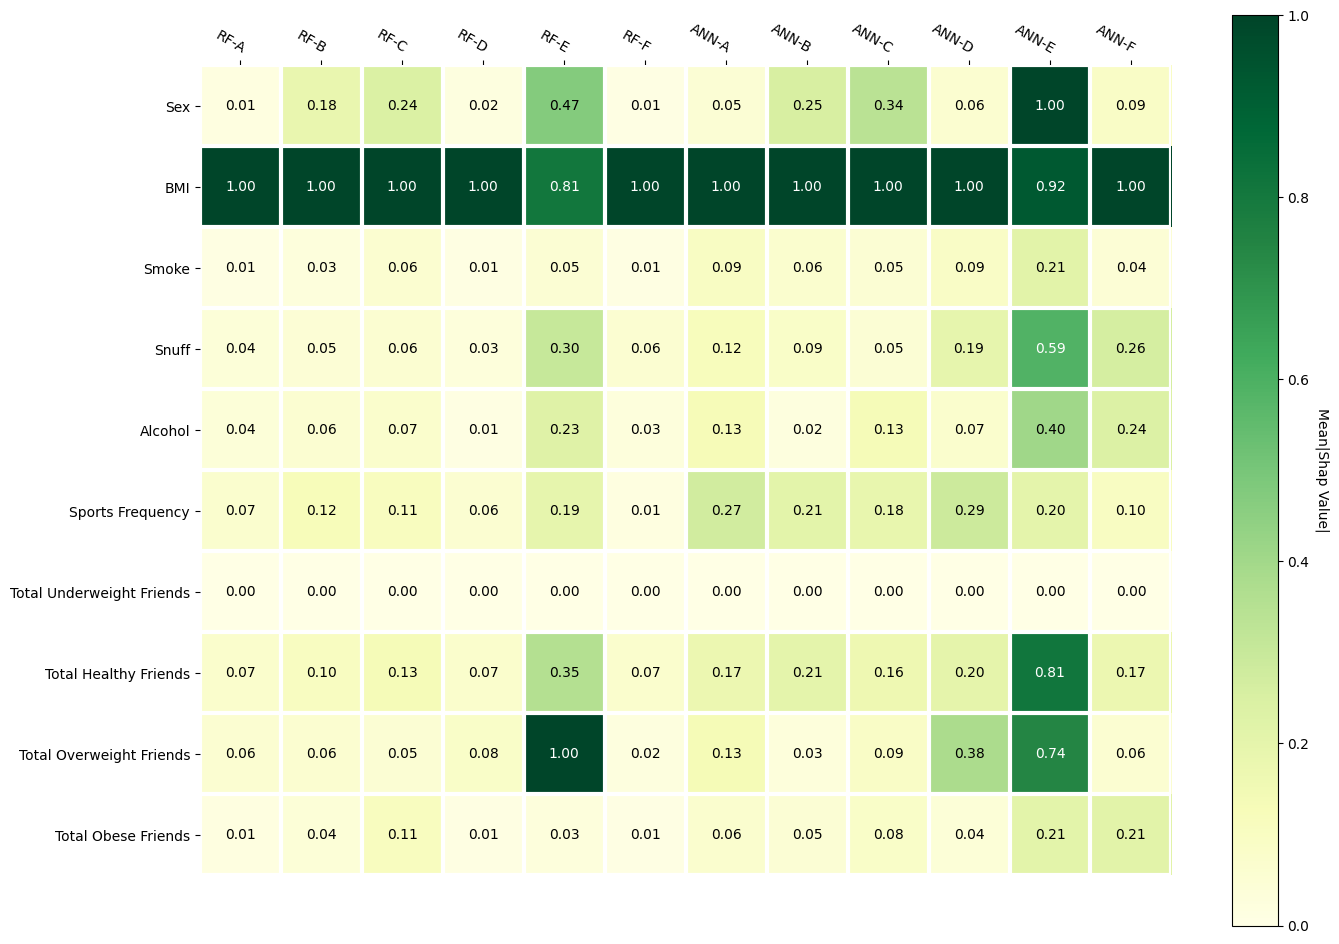
\includegraphics[width=0.9\linewidth]{figures/Results/ResultThree/Heatmap2.png } 
        \caption{Heatmap with the normalized mean |SHAP values| for the model with respect to each dataset (top names) against each variable (left names). Values closer to 1 indicate strong importance in the model.}
        \label{figure:Results3A}
    \end{figure}

    \begin{figure}[ht]
        \centering
            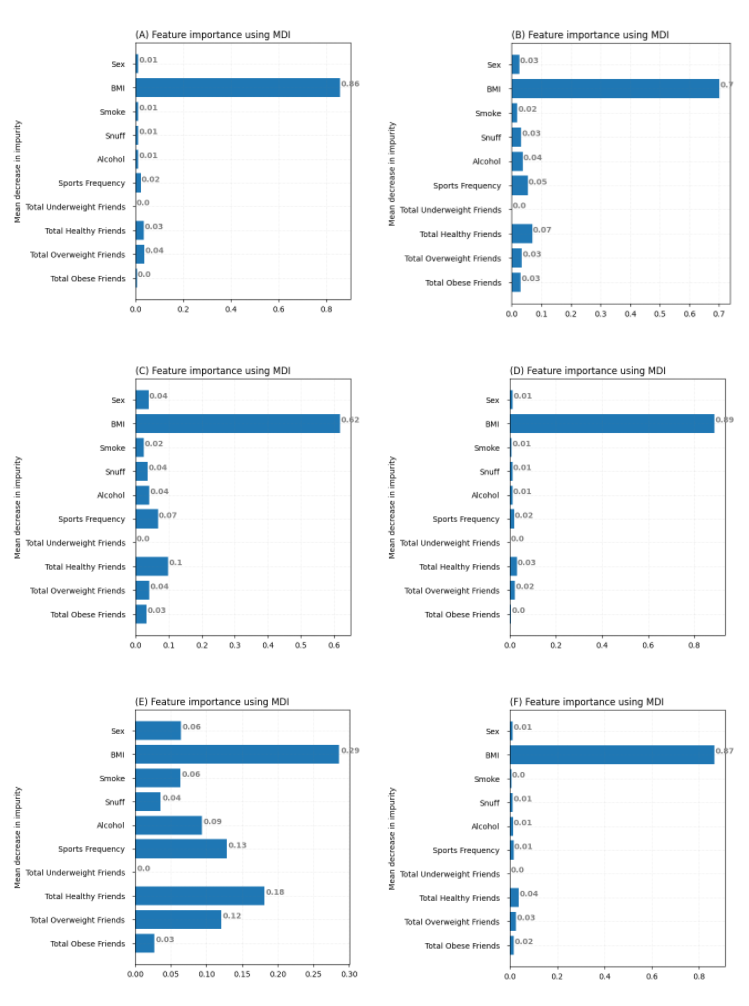
\includegraphics[width=0.9\linewidth]{figures/Results/ResultThree/MDIs.png } 
        \caption{Barplots using MDI in RF for each of the datasets. The x-axis represents the MDI value, the greater the value the greater the importance. The y-axis represents each of the studied variables.}
        \label{figure:Results3B}
    \end{figure}

It is possible to evaluate specific individuals to check what makes them gain or lose BMI in FF2 with respect to FF1. Here we present two examples using RF in dataset A (figures \ref{figure:ResultsSHAP1} and  \ref{figure:ResultsSHAP2}). Individual cases should not be extrapolated as variable weights for the whole dataset. 

    \begin{figure}[ht]
        \centering
            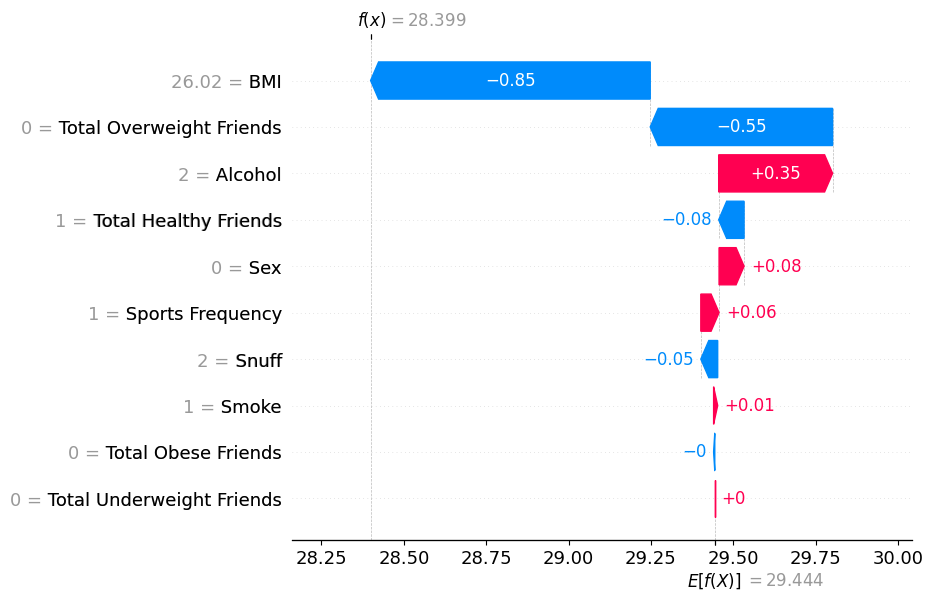
\includegraphics[width=0.9\linewidth]{figures/Results/ResultThree/Person Model RFA.png } 
        \caption{Waterfall plot with an individual case in the (A) dataset. The first row is the initial BMI in FF1, which was 26.09 (overweight) but is relatively close to 25 and this person is almost classified as healthy. This contributed the most (-0.85) to the final BMI in FF2 displayed on the figure’s top “f(x) = 28.399”, which increases below average in comparison with the rest of the samples in this dataset; with the average being 29.444 displayed on the bottom of the figure as “E[f(X)] = 29.2444”. After that, we see that having 0 overweight friends also contributed (-0.55) in favor of lowering the final BMI. The alcohol consumption of 2, equivalent to “Twice or more per month”, contributed in the opposite direction, increasing the final BMI to +0.35. One healthy friend contributed a little bit to decrease the final BMI. Being a man (sex = 0) contributed a little bit to worse BMI. And so on for the rest of the variables until the change becomes inconsequential. }
        \label{figure:ResultsSHAP1}
    \end{figure}

    \begin{figure}[ht]
        \centering
            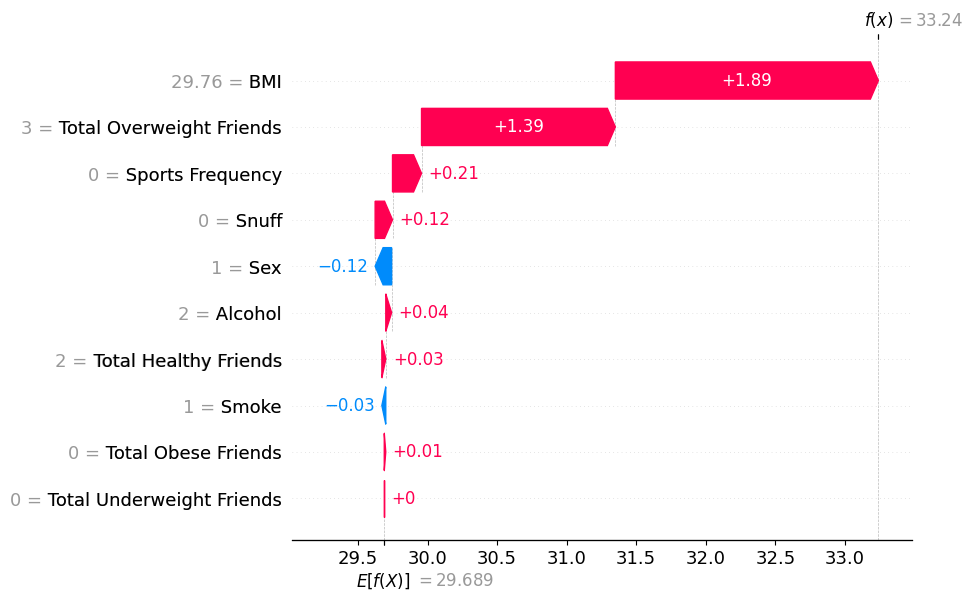
\includegraphics[width=0.9\linewidth]{figures/Results/ResultThree/Person ModelRFA 36.png} 
        \caption{Waterfall plot with an individual case in the (A) dataset. The initial BMI in FF1 was 29.68, very close to the obese category, which contributed the most to increasing the final FF2 BMI to 33.24, displayed in “f(x) = 33.24” at the top of the figure, by quite a lot (+1.89), in comparison with the FF2 average displayed at the bottom of the figure as “E[f(x)] = 29.689”. Having 3 overweight friends also contributed to a similar increase of +1.39. Not practicing any sport also contributed to a moderate increase in BMI (+0.21). The rest of the variables' effects’ sizes are quite small in comparison to the effects of the first three. }
        \label{figure:ResultsSHAP2}
    \end{figure}

Partial dependencies plots indicate how changing a particular variable changes the output of the model. All plots produced in this section are done using the RF models.

All datasets except C (Healthy to Healthy) show a decrease in BMI with respect to the total number of healthy friends (figure \ref{figure:Results3PDHealthy}). Datasets B (Overweight or Obese to better) and C also show a slight increase in BMI with sports, this might be due to an increase in muscle mass and reduced total percentage of fat due to exercise. Increasing the BMI is not necessarily bad if the increase is due to a higher weight due to increased muscle mass. So, in the C dataset, this increase seems to be justified due to staying healthy. In the B dataset, it would indicate that sports also help by decreasing total body fat. 

    \begin{figure}[ht]
        \centering
            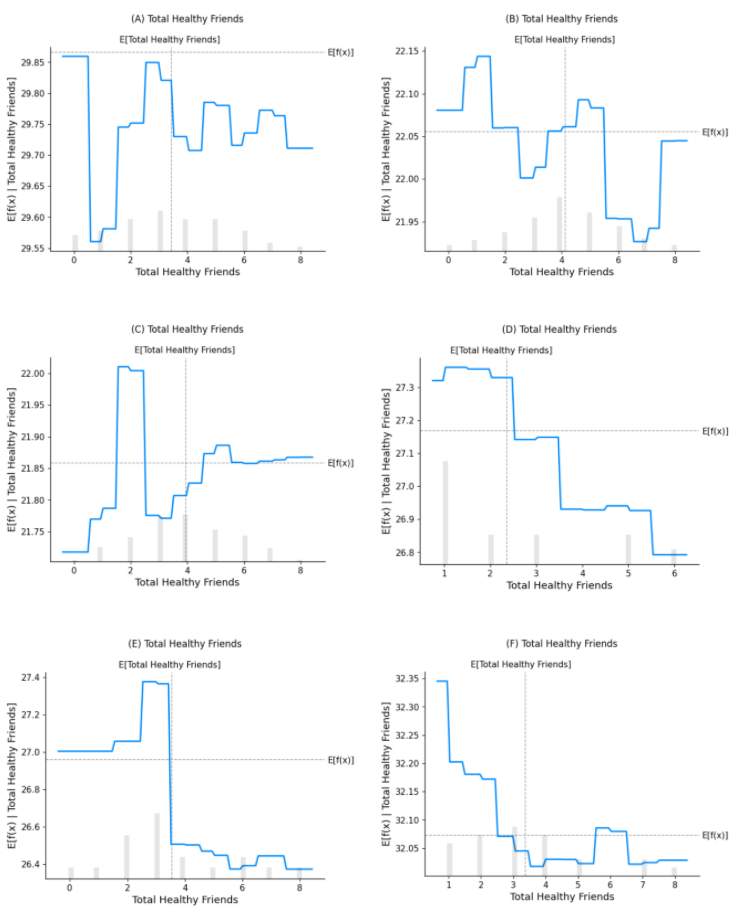
\includegraphics[width=0.9\linewidth]{figures/Results/ResultThree/PDHealthy.png } 
        \caption{Partial dependencies plots for datasets A to F in regard to total healthy friends for the RF models. On the X-axis, the total number of healthy friends, with a light grey histogram in the background. On the Y-axis, this variable is expected to modify the model output (BMI) as the variable changes.}
        \label{figure:Results3PDHealthy}
    \end{figure}

All datasets except for D (Overweight or worse got better BMI) showed an increase in BMI with respect to the total number of overweight friends (figure \ref{figure:Results3PDObese}). 

    \begin{figure}[ht]
        \centering
            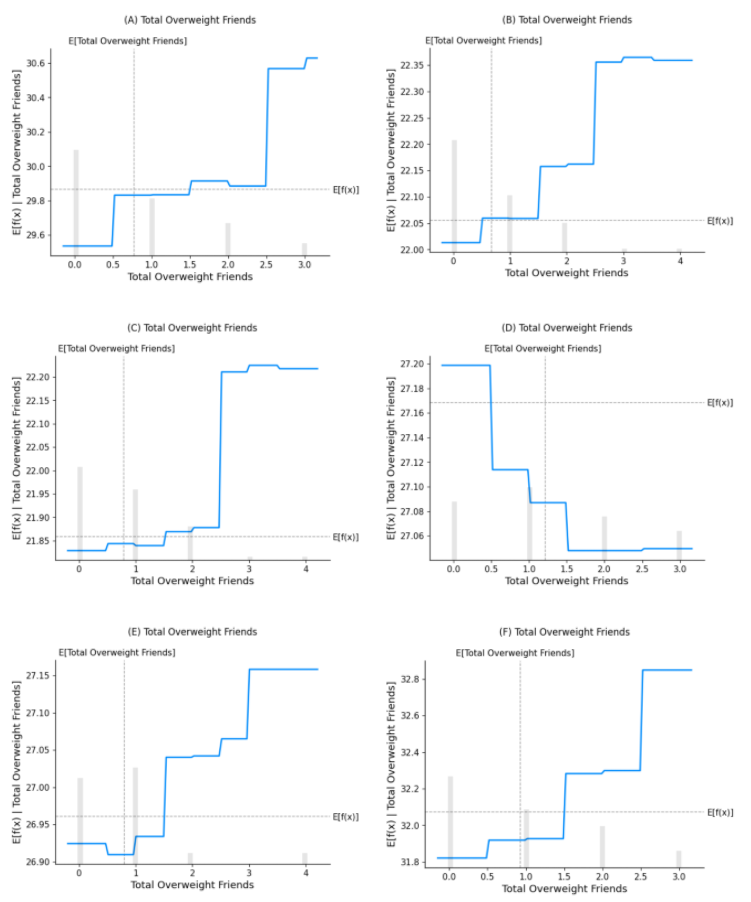
\includegraphics[width=0.9\linewidth]{figures/Results/ResultThree/PDOverweight.png } 
        \caption{Partial dependencies plots for datasets A to F in regard to total overweight friends for the RF models. On the X-axis, the total number of healthy friends, with a light grey histogram in the background. On the Y-axis, how this variable is expected to modify the model output (BMI) as the variable changes.}
        \label{figure:Results3PDObese}
    \end{figure}    

The dependency plots show on average a very slight increase (+0.12) in the final BMI. The weight of this variable is also low in the RF models. We show in the friendship bias section that obese individuals have low popularity and are not well connected with the healthy group. For all combined 692 valid samples, the average of total overweight friends is 0.28 ±0.56.  It would appear that increasing connectivity with obese individuals did not have a meaningful effect. However, since the connectivity is low, we can’t extrapolate on how the effect would be in a better-connected population. 
 
The E dataset (Healthy BMI that ends up in Overweight or worse) seems to have a completely different weight of SHAP values according to both RF and ANN (figure \ref{figure:Results3A}), and to MDI in RF (figure \ref{figure:Results3B}). Is also the group with the bigger BMI increase (+3.2 ±1.6). The variable Total Overweight friends get a very high impact on the model despite people not having that many overweight friends. In general, Total Healthy friends decrease the BMI but it shows a spike in BMI for specifically “3” healthy friends (figure \ref{figure:Results3PDHealthy}).  It shows an increase with smoke but a decrease with snuff and alcohol frequency (figure \ref{figure:Results3EWeird}). Females have slightly more risk than males. We tried limiting the dataset from Healthy to Overweight only in case the Healthy to Obese jump was too much of an outlier, but it had barely any effect on the outputs. Analyzing all individuals one by one using the waterfall plots did not show any pattern. Dataset C shows a spike in BMI for “2” total numbers of healthy friends (figure \ref{figure:Results3PDHealthy}), but the model is more predictable. E is just a subset of the A dataset which does not show any strange particularities either. 

    \begin{figure}[ht]
        \centering
            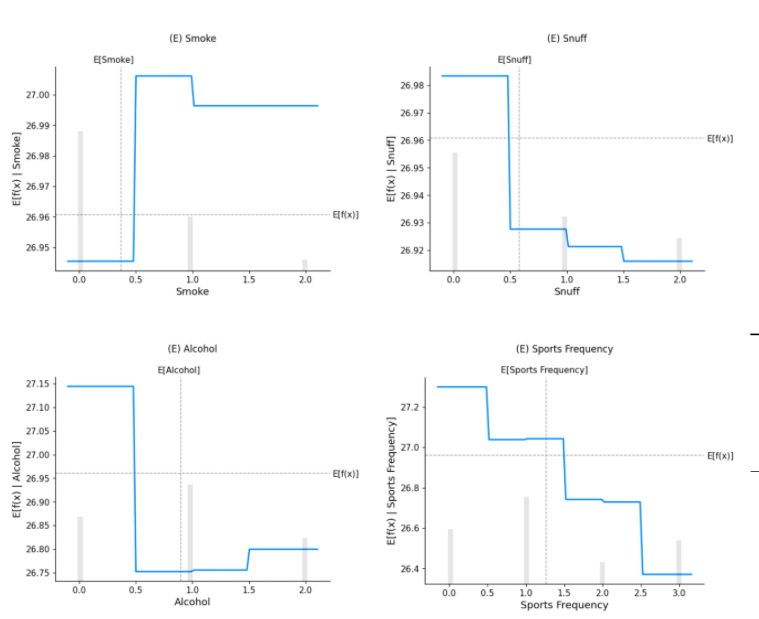
\includegraphics[width=0.7\linewidth]{figures/Results/ResultThree/PDECrap.png } 
        \caption{Partial dependencies plots for datasets E regarding recreational drugs and sport frequency for the RF models. On the X-axis, the total number of healthy friends, with a light grey histogram in the background. On the Y-axis, how this variable is expected to modify the model output (BMI) as the variable changes. }
        \label{figure:Results3EWeird}
    \end{figure}    

Similarly to Result I, here we evaluate the influence of friendship on obesity and it appears that there's also an influence depending on the number of "Healthy", "Overweight", or "Obese" friends. And our machine learning models give a similar explanation compared with previous results.

\clearpage



\section{Result IV}

\textbf{Frequency consumption of medication and social network influence in a general youth population.}

In previous studies there has been a concerning trend in self-medication and in particular the overuse of painkillers for non-therapeutic purposes; mostly as a recreational drug within Norway \cite{ref:selfMedicationA, ref:selfMedicationB, Lorentzen2018} which coincide with worldwide trends and usage \cite{Algarni2021, ijerph18115530, PolandSelfMedicate, Lein2023}. With this study, we aim for two objectives. First, to update the data on self-reporting medication with the FF1's 2010 data, and if possible, include up to Fit Futures 3 data done throughout the year 2022. And second to investigate if there's a social influence component as to whether students tend to self-medicate.

% and \ref{figure:Results4D}, unreferenced, taken away

We analyzed the frequency of self-reported consumption of medicines and diseases in our population (figure \ref{figure:Results4C}). We can observe that there are plenty of dermatological diseases, however, the usage of dermatological medicines is quite low. In contrast, the amount of pain-related diseases is low, but the consumption of painkillers, or anti-inflammatory medicaments is extremely high in comparison.

    \begin{figure}[H]
        \centering
            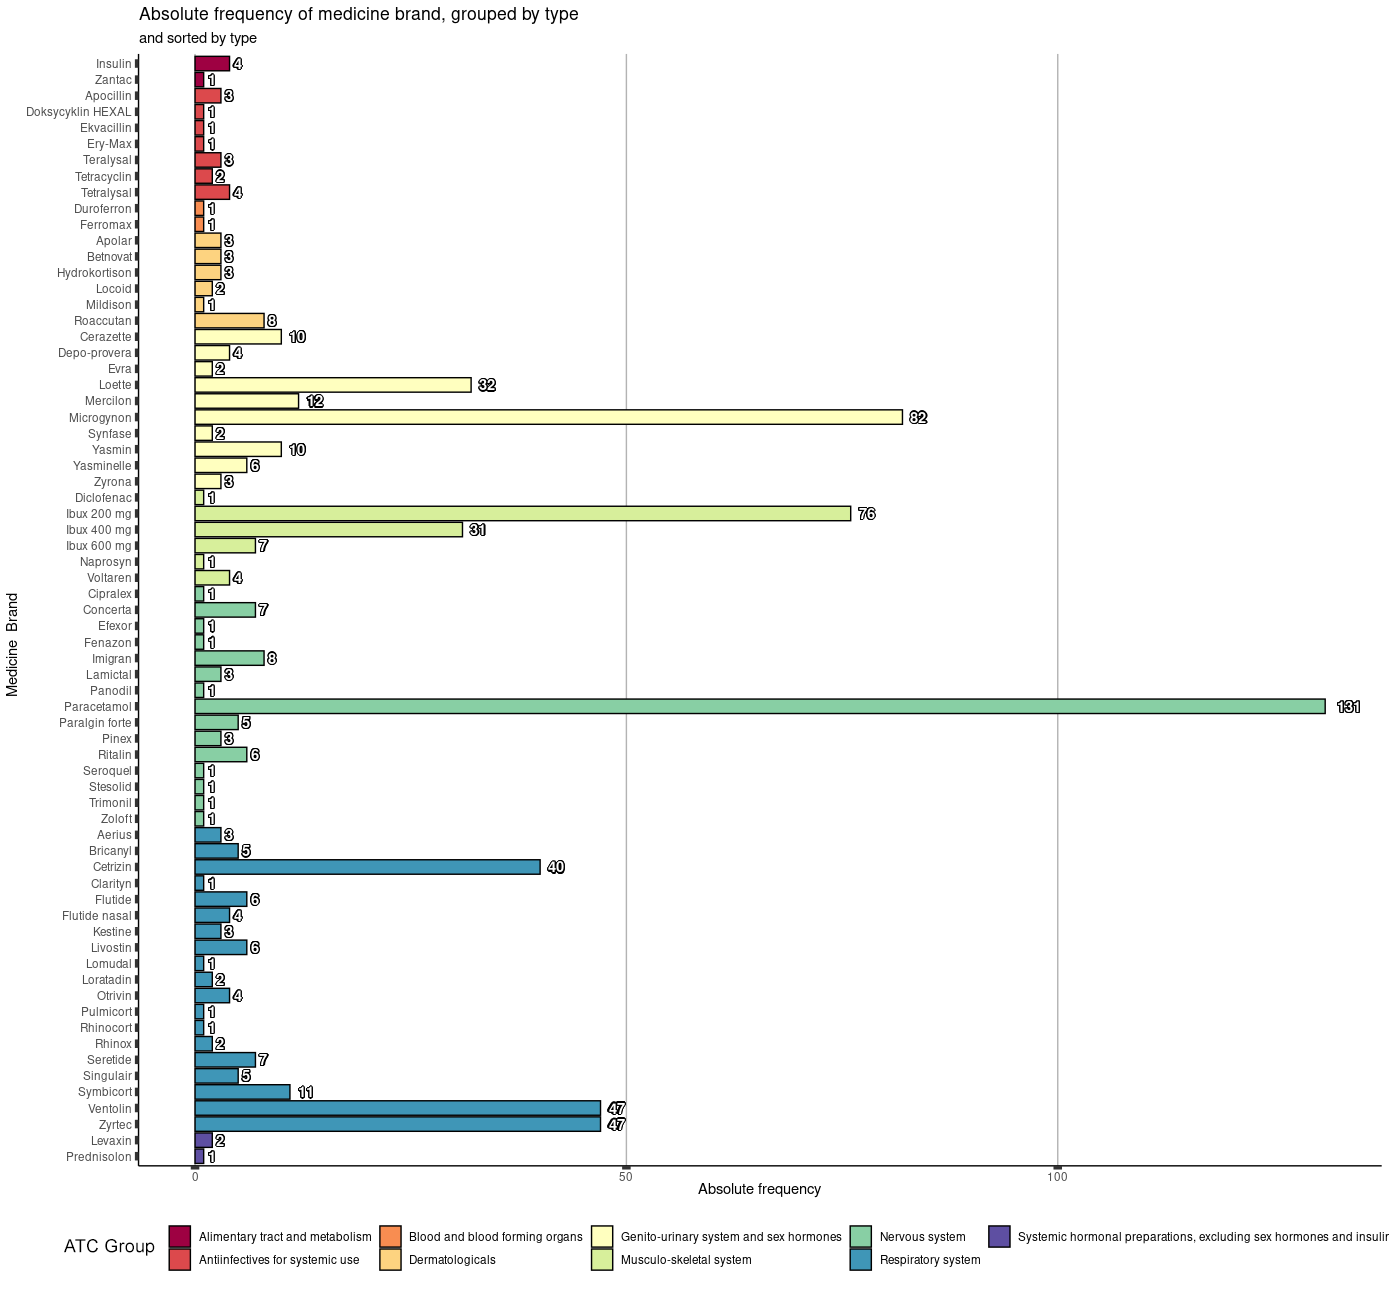
\includegraphics[width=0.9\linewidth]{figures/Results/ResultFour/CombinedLongRelBarPlot_typesAbsolute_Brand_TypeType.png } 
        \caption{Absolute frequency of medicine consumption sorted by ATC group. Hormonal contraceptives, anti-inflammatories, painkillers, antiasthmatic, and antihistaminics dominate the frequency of use.}
        \label{figure:Results4C}
    \end{figure}

Females seem to have a higher consumption of medicines in general (figure \ref{figure:Results4B}), and also higher disease prevalence (figure \ref{figure:Results4Diseases}). However, the disease types and medicine types don't match; meaning that self-medication is higher among the female population.

    \begin{figure}[H]
        \centering
            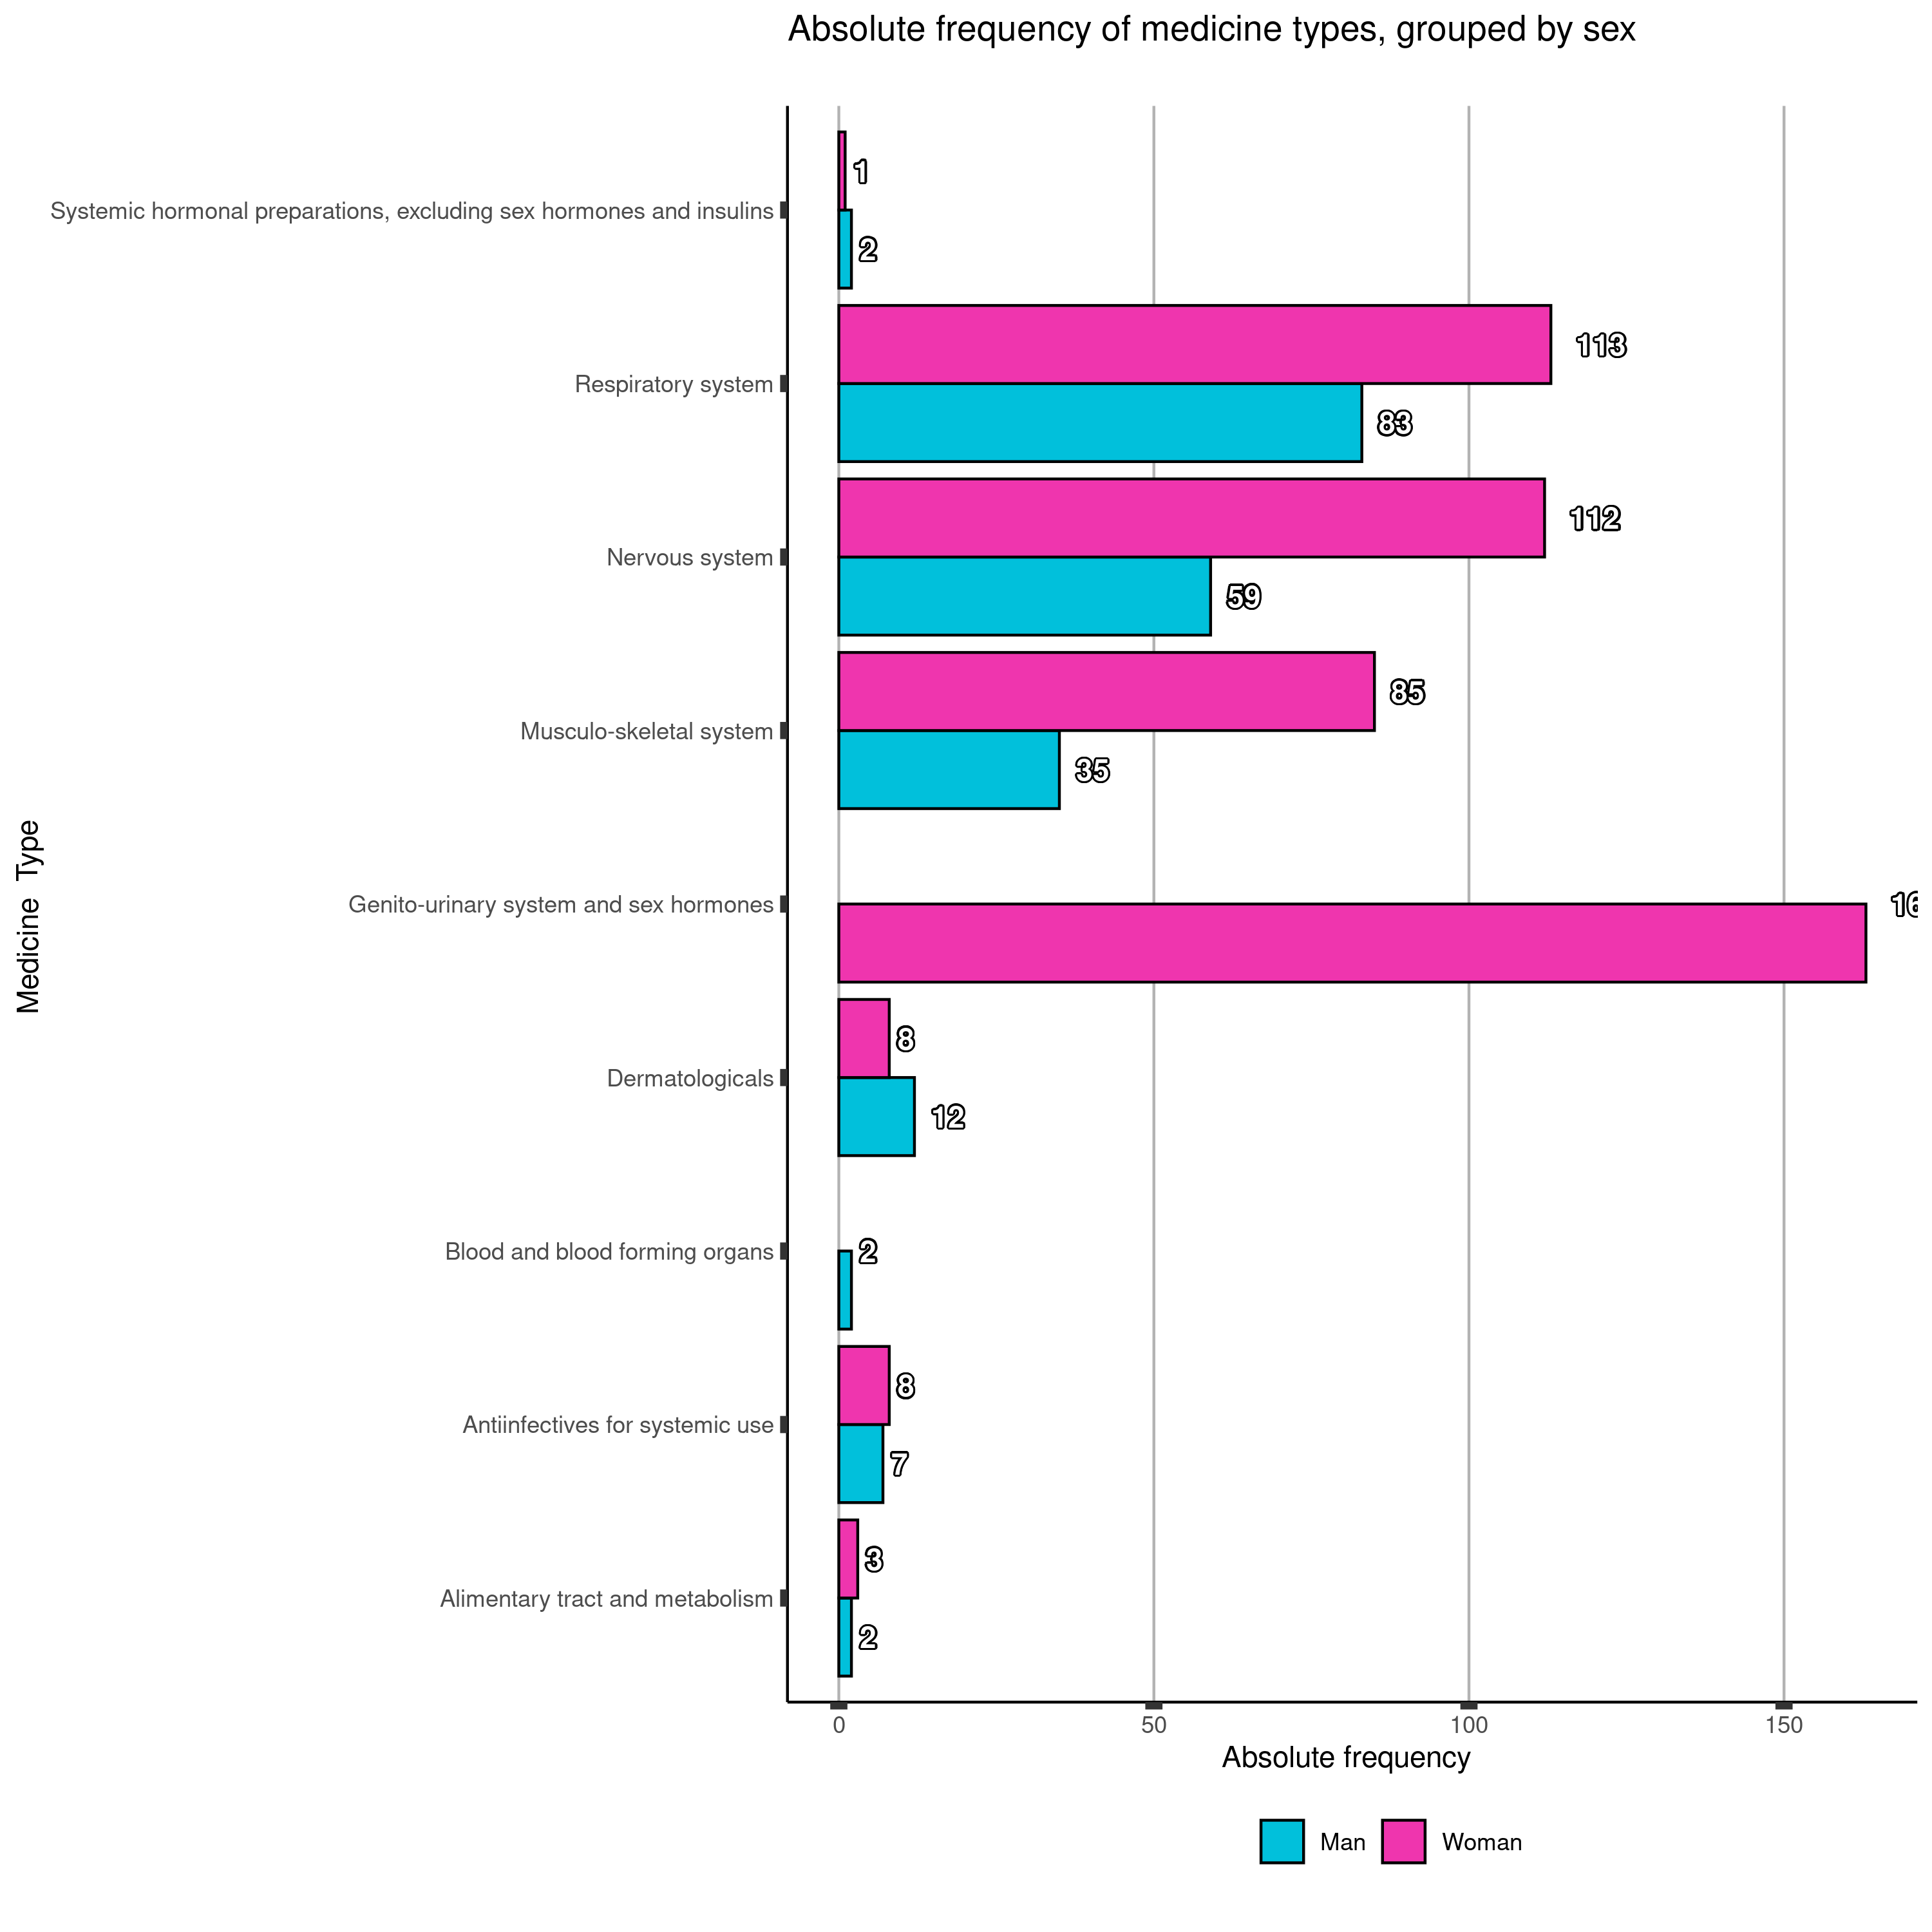
\includegraphics[width=0.9\linewidth]{figures/Results/ResultFour/CombinedLongAbsBarPlot_typesBySex_Type_Sex.png } 
        \caption{Absolute frequency of medicine consumption group by ATC group and divided by sex, which seems to indicate a higher consumption among females}
        \label{figure:Results4Diseases}
    \end{figure}

    
    \begin{table}
    
        \caption{Summary of the $Xi^2$ significance for relevant medicine groups divided by bias type (high school and sex). From left to right, bias type, type of medicine, numerical significance rounded to 4 decimals, and p-value in GP Prism 5.04/d format. Hormonal contraceptives seem to be biased concerning high school. Painkillers also seem to be biased by high school and sex. Anti-inflammatory shows a bias by sex only}
        
        \centering
        
        \begin{tabular}{clll}
        
            \rowcolor[rgb]{1,1,0.78} \multicolumn{1}{l}{Bias type}       & Medicine                             & Significance &       \\ 
            \hline
            {\cellcolor[rgb]{1,0.808,0.576}}                             & Hormonal contraceptives (women only) & 0.0002       & ***   \\
            {\cellcolor[rgb]{1,0.808,0.576}}                             & Anti-inflammatory                    & 0.2075       & ns    \\
            {\cellcolor[rgb]{1,0.808,0.576}}                             & Antihistamine                        & 0.1766       & ns    \\
            \multirow{-4}{*}{{\cellcolor[rgb]{1,0.808,0.576}}Highschool} & Painkiller                           & 0.0006       & ***   \\ 
            \hline
            {\cellcolor[rgb]{0.925,0.957,1}}                             & Anti-inflammatory                    & 0            & ****  \\
            {\cellcolor[rgb]{0.925,0.957,1}}                             & Antihistamine                        & 0.264        & ns    \\
            \multirow{-3}{*}{{\cellcolor[rgb]{0.925,0.957,1}}Sex}        & Painkiller                           & 0.0011       & **   
            
        \end{tabular}
        
        \label{table:Results4XiSummary}
        
    \end{table}

    \begin{figure}[H]
        \centering
            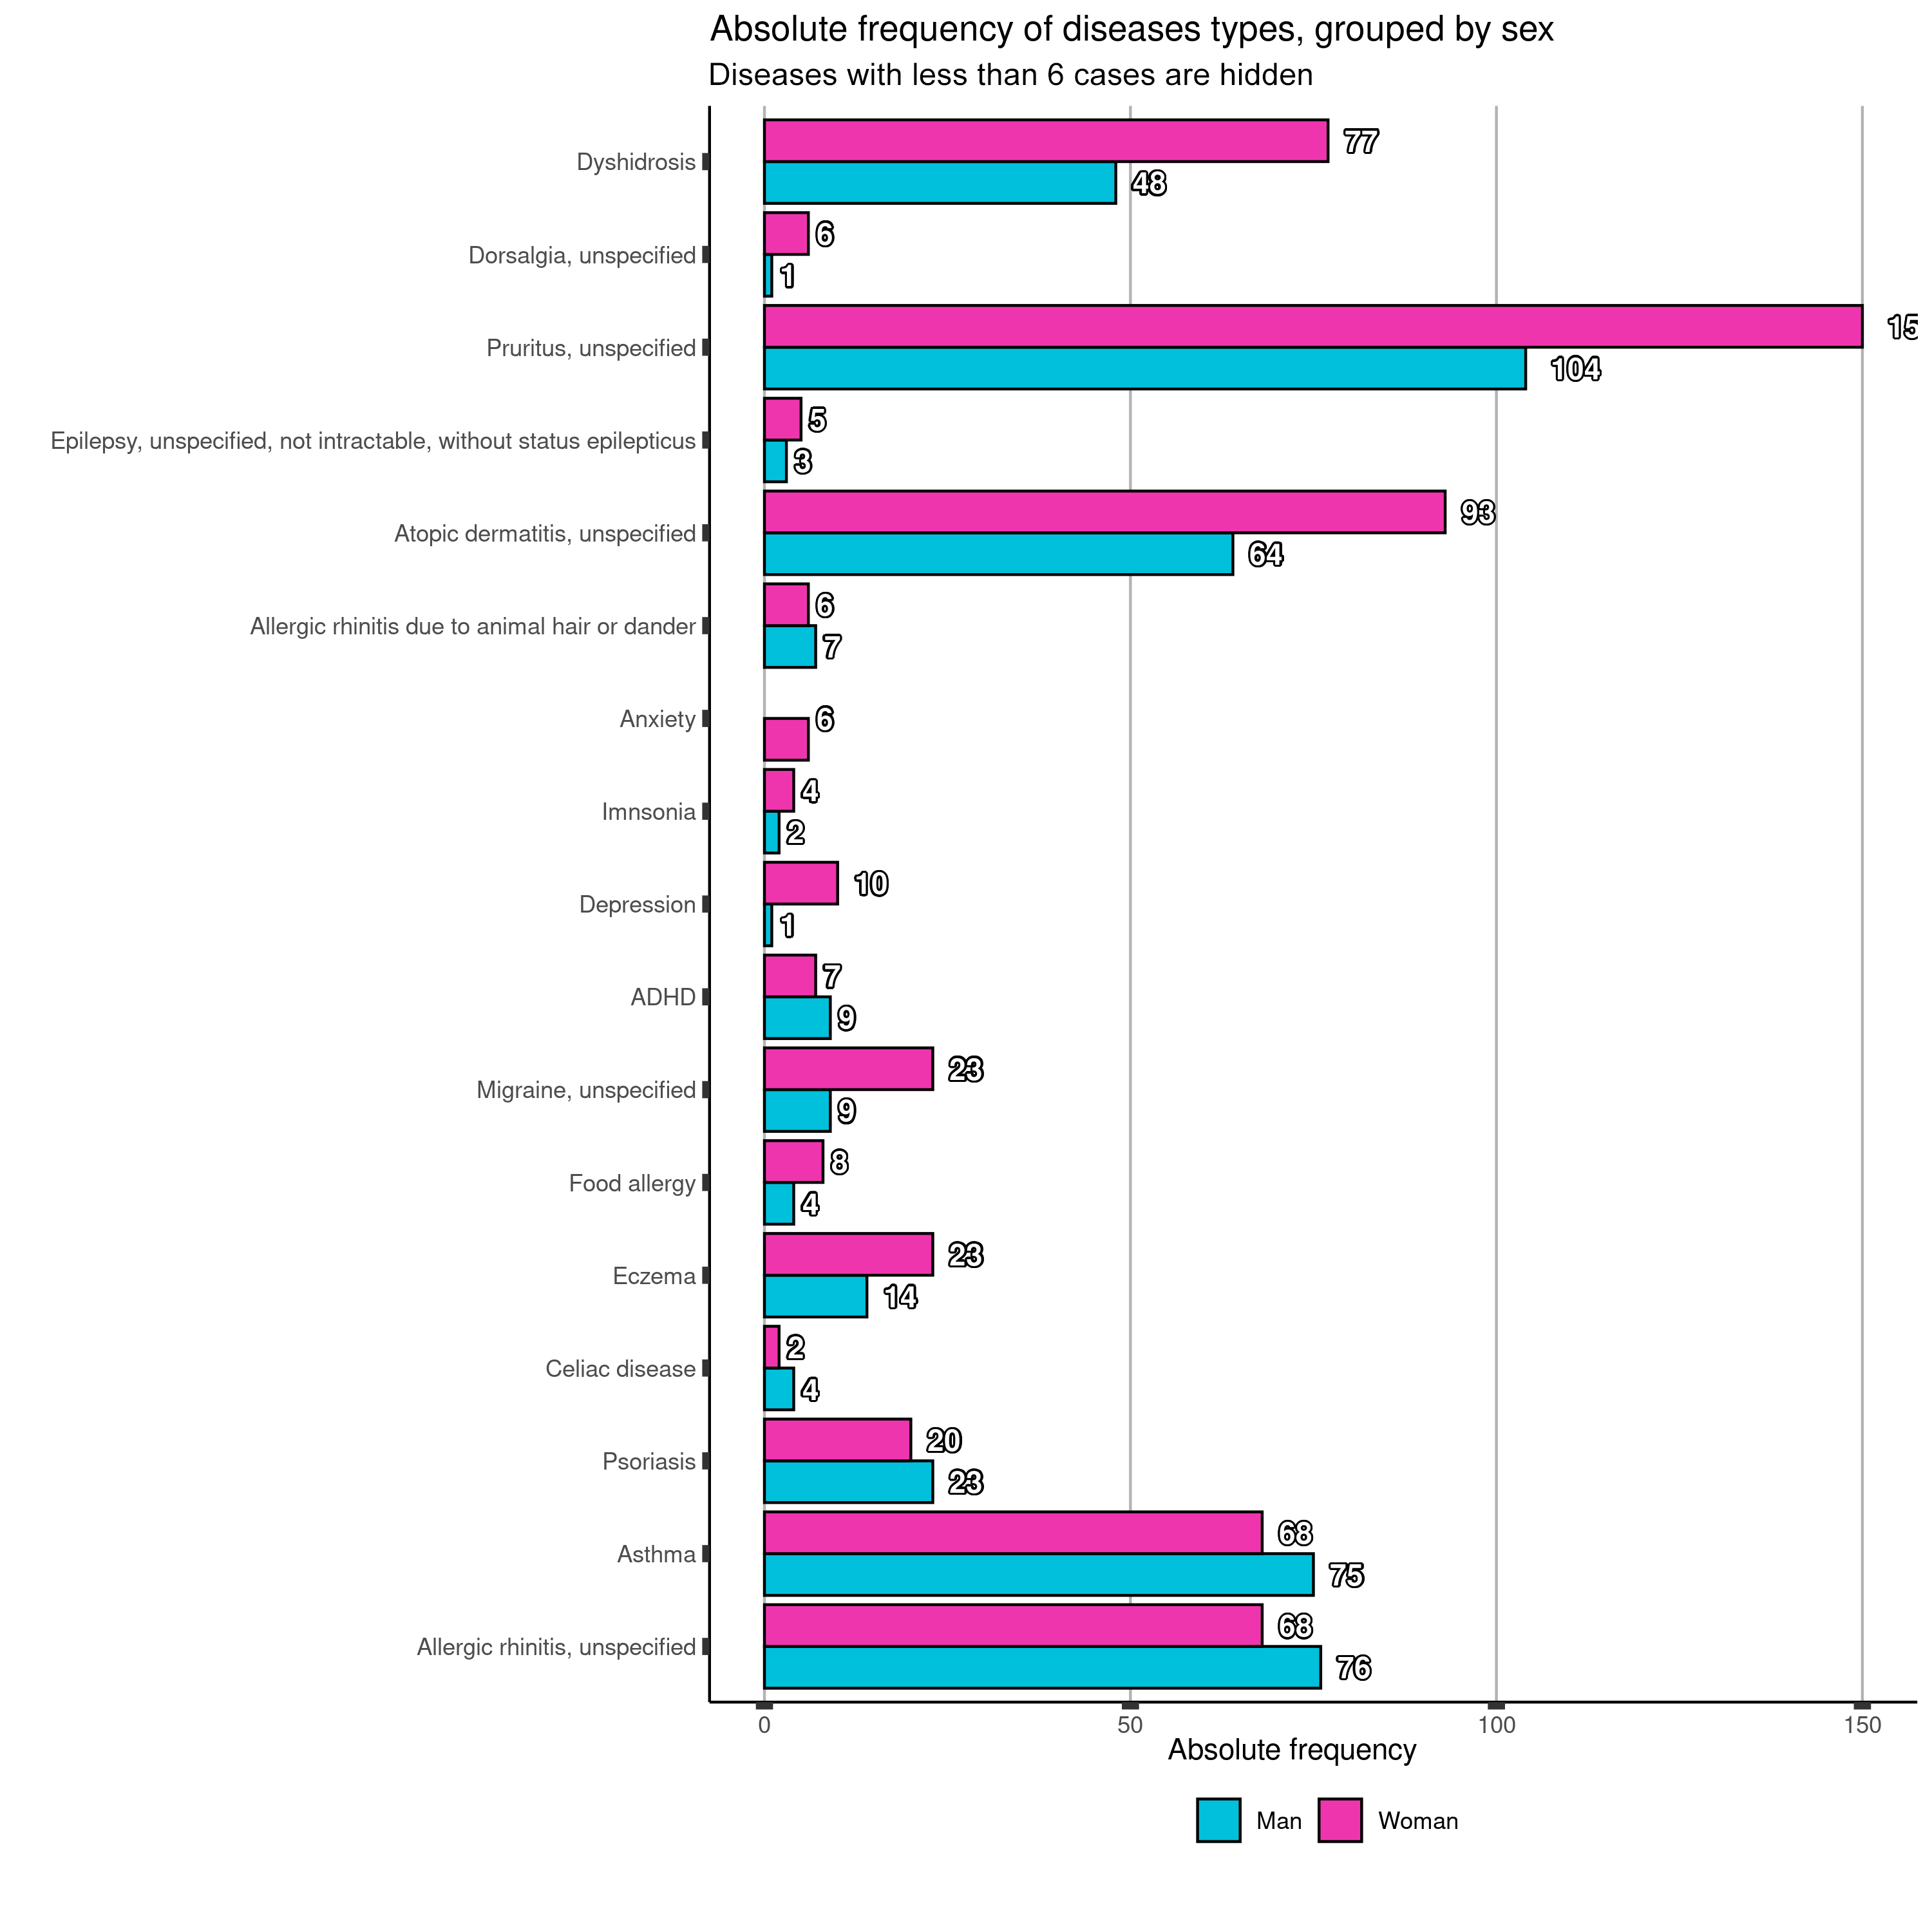
\includegraphics[width=0.9\linewidth]{figures/Results/ResultFour/CombinedLongAbsBarPlot_typesDiseasesBySex_Diagnostic_Sex.png } 
        \caption{Absolute frequency of self-reported diseases divided by sex. To avoid visual cluttering, diseases with 5 or fewer instances are not included in this figure. Females also lead in dermatological and psychological conditions, plus migraines. Males seem to have a short lead in respiratory conditions.}
        \label{figure:Results4B}
    \end{figure}

    %\begin{figure}[H]
     %   \centering
      %      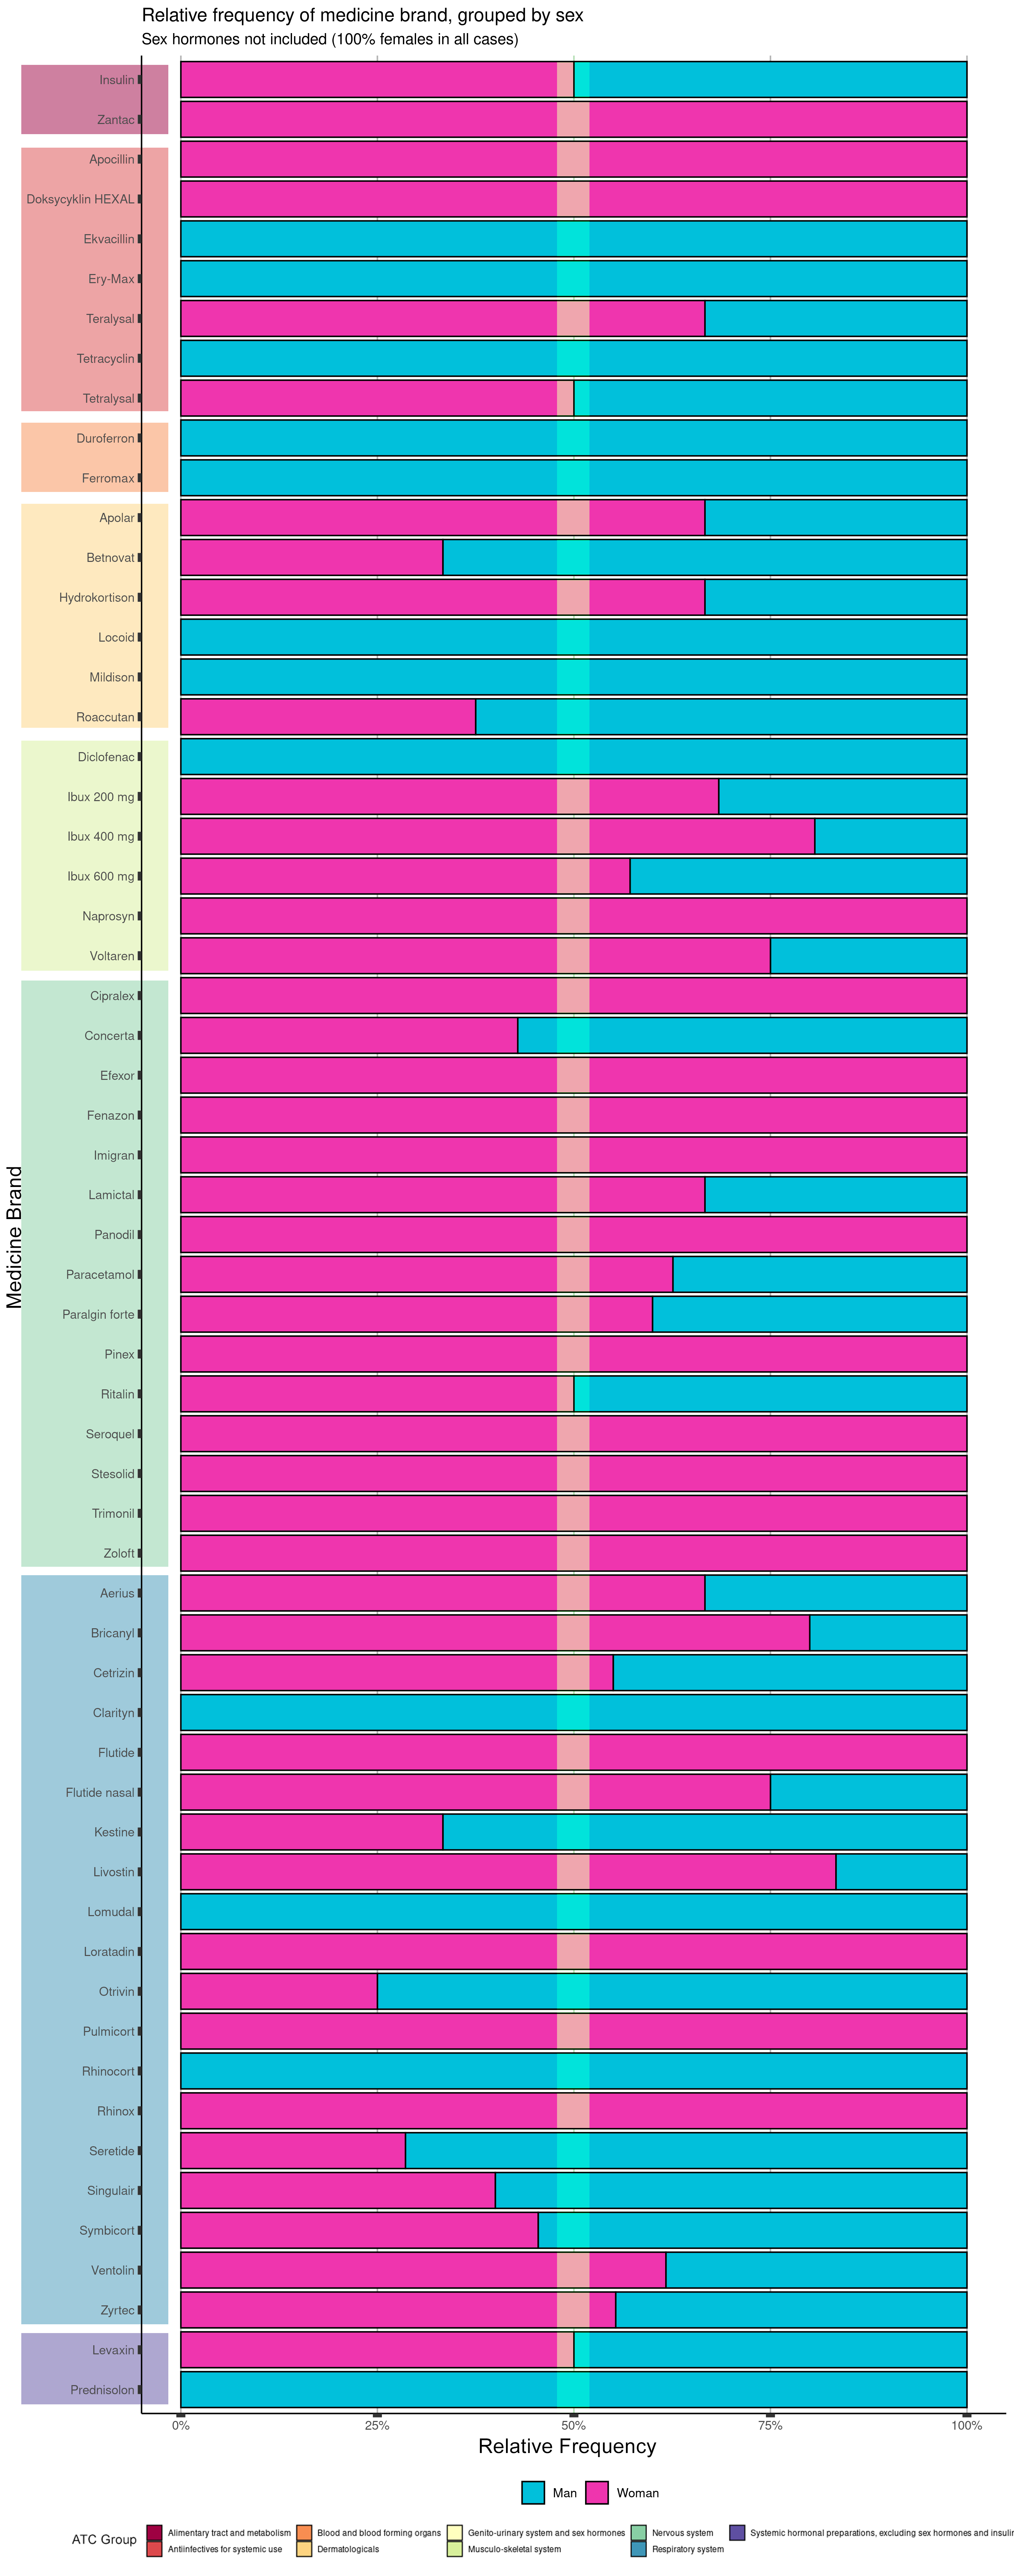
\includegraphics[width=0.5\linewidth]{figures/Results/ResultFour/CombinedLongRelBarPlot_typesBySex_Brand_Sex2.png } 
       % \caption{Relative consumption of medicines grouped by brand and divided by sex. Hormonal contraceptives are not included in the figure (100\% female). A highlight of ±5\% centered in the middle is included. Women seem to have a higher reported consumption of the most popular medicament.}
        %\label{figure:Results4D}
    %\end{figure}

We analyzed if there was any bias concerning sex and high school using over-the-counter medicines and also concerning hormonal contraceptives in women. Our results (table \ref{table:Results4XiSummary}) indicate that women sharing the same high school is biased towards hormonal contraceptive usage. Our simulations also show that women who are friends are biased to share the same hormonal contraceptive brand. One of the possible reasons is due to direct recommendations among them and later on asking their family doctor for the same brand. Another one is that women going to the same school tend to live close by and thus share the same family doctor who tends to prescribe the same medication.



The results coincide with teenagers' trend of misusing over-the-counter medication.


% Database schema and tables
%\chapter{Technical data information}
\label{chapter:Annexes}

\subsection{Database schema}
\label{chapter:Annex_schema}

This section provides an overview of all the tables that compose the data once the cleaning process is finished.

The first listing of tables corresponds to the information stored for each individual. The tables are divided by topics for better understanding, but mathematically, they should all be joined together by ID to create a large table for each of the FF time points (FF1, FF2, etc...).

\begin{sloppypar}
\begin{itemize}
    \item {Basic} (\textbf{ID}, Attendance Date FF1, Attendance Date FF12, Medication Date FF1, Questionary Date FF1, Sex, Age, General Health, Age FF12)

    \item {Network Technical} (\textbf{ID}, Signature FF1, Comment, Signature FF12, Comment FF12)
    
    \item {Antropometric FF1} (\textbf{ID}, Waist, Hip, Height, Weight, BMI, HR, SYSBP, DIABP, BMI Categorical)
    
    \item {Antropometric FF2} (\textbf{ID}, Waist, Hip, Height, Weight, BMI, HR, SYSBP, DIABP, BMI Categorical)

    \item {Aureus} (\textbf{ID}, S1 AttendanceDate, S1 R2 AttendanceDate, S2 AttendanceDate, S1 CultureDate, S2 CultureDate, S1 BacterialNasalGrowth, S1 BacterialThroatGrowth, S2 BacterialNasalGrowth, S2 BacterialThroatGrowth, S1 SA Direct NasalGrowth, S1 SA Direct ThroatGrowth, S1 SA Direct NasalPopulation, S1 SA Direct ThroatPopulation, S2 SA Direct NasalGrowth, S2 SA Direct ThroatGrowth, S2 SA Direct NasalPopulation, S2 SA Direct ThroatPopulation, S1 SA Enrich NasalGrowth, S1 SA Enrich ThroatGrowth, S1 SA Enrich NasalPopulation, S1 SA Enrich ThroatPopulation, S2 SA Enrich NasalGrowth, S2 SA Enrich ThroatGrowth, S2 SA Enrich NasalPopulation, S2 SA Enrich ThroatPopulation, S1 Direct CoagulaseNasal, S1 Direct CoagulaseThroat, S1 Enrich CoagulaseNasal, S1 Enrich CoagulaseThroat, S2 Direct CoagulaseNasal, S2 Direct CoagulaseThroat, S2 Enrich CoagulaseNasal, S2 Enrich CoagulaseThroat, SPANasal1, SPANasal2, SPAThroat1, SPAThroat2, SPAThroatClonning, SPAThroatCount, S1 D NasalColonize, S1 D ThroatColonize, S1 D Colonize, S1 E NasalColonize, S1 E ThroatColonize, S1 E Colonize, S2 D NasalColonize, S2 D ThroatColonize, S2 D Colonize, S2 E NasalColonize, S2 E ThroatColonize, S2 E Colonize, D NasalCarrier, D ThroatCarrier, D Carrier, E NasalCarrier, E ThroatCarrier, E Carrier, P Nasal, P Throat, P Carrier)

    \item {Swabbing} (\textbf{ID}, S1 NasalOK, S1 ThroatOK, S1 LabComments Enrich, S1 LabComments Staph, S1 Performed, S1 Event, S1 Medical Event, S1 Medical Event Comment, S1 Technical Event, S1 Technical Event Comment, S1 Abort Event, S1 Abort Event Comment, S1 Other Event, S1 Other Event Comment, S2 Performed, S2 Event, S2 Medical Event, S2 Medical Event Comment, S2 Technical Event, S2 Technical Event Comment, S2 Abort Event, S2 Abort Event Comment, S2 Other Event, S2 Other Event Comment, S1 Repeated Performed, S1 Nose Repeated, S1 Throat Repeated, S1 Repeated Event, S1 Repeated Medical Event, S1 Repeated Medical Event Comment, S1 Repeated Technical Event, S1 Repeated Technical Event Comment, S1 Repeated Abort Event, S1 Repeated Abort Event Comment, S1 Repeated Other Event, S1 Repeated Other Event Comment, S1 Nasal FreezeDate, S1 Throat FreezeDate, S1 FreezerNasalID, S1 FreezerThroatID, S2 FreezerNasalID, S2 FreezerThroatID)

    \item {High School} (\textbf{ID}, HighSchool, Class, Programme, MainPrograme)
    
    \item {Blood} (\textbf{ID}, Blood Analysis Date, Plasma Analysis Date, Time Since Eating, Mean Corposcular Hemoglobin pg, Mean Corposcular Hemoglobin Concentration g dL, Mean Corposcular Hemoglobin Volume fl, Fe µmol L, Ferritinin ug L, Transferrin g L, Total cholesterol mmol L, Triglycerides mmol L, LDL cholesterol mmol L, HDL cholesterol mmol L, Calcium mmol L, High sensitive CRP, Apolipoprotein A1 g L, Apolipoprotein B g L, Estradiol E2 nmol L, Progesterone nmol L, Testosterone nmol L, DHEA SO4 µmol L, SHBG nmol L, LH IU L, FSH IU L, Glucose Non fasting mmol L, HBA1C ..., Haemoglobin g dL, Albumin g L, X25 OH D nmol L, Retinol µmol L, PTH pmol L, FA C12 0 mcg ml, FA C14 0 mcg ml, FA C15 0 mcg ml, FA C16 0 mcg ml, FA C16 1 n 7 mcg ml, FA C18 0 mcg ml, FA C18 1 t6 11 mcg ml, FA C18 1 c 9 mcg ml, FA C18 1 c 11 mcg ml, FA C18 2 n 6 mcg ml, FA C20 0 mcg ml, FA C18 3 n 6 mcg ml, FA C18 3 n 3 mcg ml, FA C20 1 n 9 mcg ml, FA C20 2 n 6 mcg ml, FA C22 0 mcg ml, FA C20 3 n 6 mcg ml, FA C20 4 n 6 mcg ml, FA C23 0 mcg ml, FA C20 5 n 3 mcg ml, FA C24 0 mcg ml, FA C24 1 mcg ml, FA C22 5 n 3 mcg ml, FA C22 6 n 3 mcg ml, FA C12 0 weight, FA C14 0 weight, FA C15 0 weight, FA C16 0 weight, FA C16 1 n 7 weight, FA C18 0 weight, FA C18 1 t6 11 weight, FA C18 1 c 9 weight, FA C18 1 c 11 weight, FA C18 2 n 6 weight, FA C20 0 weight, FA C18 3 n 6 weight, FA C18 3 n 3 weight, FA C20 1 n 9 weight, FA C20 2 n 6 weight, FA C22 0 weight, FA C20 3 n 6 weight, FA C20 4 n 6 weight, FA C23 0 weight, FA C20 5 n 3 weight, FA C24 0 weight, FA C24 1 weight, FA C22 5 n 3 weight, FA C22 6 n 3 weight)
    
    \item {Blood Technical} (\textbf{ID}, Blood Test Performed, Blood Event, Blood Medical Event, Blood Medical Comment, Blood Technical Event, Blood Technical Comment, Blood Aborted, Blood Aborted Comment, Blood Other, Blood Other Comment, Blood S25OH Event, Blood S25OH Event Comment, Blood Retinol Event, Blood Retinol Event Comment)

    \item {Sociology} (\textbf{ID}, Live With Mother, Live With Father, Live With Stepfather, Live With Stepmother, Live With Foster Parents, Live With Adoptive Parents, Live With Grandparents, Live With Friends, Live With Nobody, Live With Institution, Live With Other, When Left Home, Mother Work Time, Mother Studying, Mother Domestic, Mother Disable, Father Work Time, Father Studying, Father Domestic, Father Disable, Mother Education, Father Education, Ethnicity, Live With Siblings)
    
    \item {Frienship Table} (\textbf{ID}, Created, Overview, Yesterday SMS, Overall Connections, Overall Popularity, Overall Following, Overall Reciprocity, Physical Connections, Physical Popularity, Physical Following, Physical Reciprocity, School Connections, School Popularity, School Following, School Reciprocity, Sports Connections, Sports Popularity, Sports Following, Sports Reciprocity, Home Connections, Home Popularity, Home Following, Home Reciprocity, Other Connections, Other Popularity, Other Following, Other Reciprocity, Overall Connections FF12, Overall Popularity FF12, Overall Following FF12, Overall Reciprocity FF12, Physical Connections FF12, Physical Popularity FF12, Physical Following FF12, Physical Reciprocity FF12, School Connections FF12, School Popularity FF12, School Following FF12, School Reciprocity FF12, Sports Connections FF12, Sports Popularity FF12, Sports Following FF12, Sports Reciprocity FF12, Home Connections FF12, Home Popularity FF12, Home Following FF12, Home Reciprocity FF12, Other Connections FF12, Other Popularity FF12, Other Following FF12, Other Reciprocity FF12)
    
    \item {Puberty Men Table} (\textbf{ID}, Change Height, Change Voice, Facial Hair, Men Body Hair, Men Pubic Hair, Men Pubic Age)
    
    \item {Puberty Women Table} (\textbf{ID}, Menarche, Menarche Age, Women Pubic Hair, Breasts)

    \item {Menstruation} (\textbf{ID}, Date, Menstruation Start, Menstruation Regular, Menstruation Cycle, Menstruation Date, Cycle Advance)
    
    \item {Drugs Table} (\textbf{ID}, Smoke, Smoke Per Week, Smoke Per Day, Snuff, Snuff Per Week, Snuff Per Day, Alcohol, Alcohol Units, Alcohol 6 Units)

    \item {Sports} (\textbf{ID}, Sports Leisure, Sports Outside School, Sports Frequency, Sport Hours, Sports Intensity, Summer Transport, Summer Time, Winter Transport, Winter Time, Screen Time)
    
    \item {Hygiene} (\textbf{ID}, Shower Bath Frequency, Handwash Frequency, Body Lotion Frequency, Skin Sunbathing, Holiday Sunbathing, Solarium Last 4 Weeks) 
    
    \item {Biomarkers} (\textbf{ID}, BatchNumber, Flagged, Adenosine Deaminase LOD, Artemin LOD, Axin 1 LOD, Brain derived neurotrophic factor LOD, Beta nerve growth factor LOD, Caspase 8 LOD, Eotaxin LOD, CC motif chemokine 19 LOD, CC motif chemokine 20 LOD, CC motif chemokine 23 LOD, CC motif chemokine 25 LOD, CC motif chemokine 28 LOD, CC motif chemokine 3 LOD, CC motif chemokine 4 LOD, Natural killer cell receptor 2B4 LOD, CD40L receptor LOD, T cell surface glycoprotein CD5 LOD, T cell surface glycoprotein CD6 isoform LOD, CUB domain containing protein 1 LOD, Macrophage colony stimulating factor 1 LOD, Cystatin D LOD, Fractalkine LOD, CXC motif chemokine 1 LOD, CXC motif chemokine 10 LOD, CXC motif chemokine 11 LOD, CXC motif chemokine 5 LOD, CXC motif chemokine 6 LOD, CXC motif chemokine 9 LOD, Delta and Notch like epidermal growth factor related receptor LOD, Eukaryotic translation initiation factor 4E binding protein 1 LOD, Protein S100 A12 LOD, Fibroblast growth factor 19 LOD, Fibroblast growth factor 21 LOD, Fibroblast growth factor 23 LOD, Fibroblast growth factor 5 LOD, Fms related tyrosine kinase 3 ligand LOD, Glial cell line derived neurotrophic factor LOD, Hepatocyte growth factor LOD, Interferon gamma LOD, Interleukin 10 LOD, Interleukin 10 receptor subunit alpha LOD, Interleukin 10 receptor subunit beta LOD, Interleukin 12 subunit beta LOD, Interleukin 13 LOD, Interleukin 15 receptor subunit alpha LOD, Interleukin 17 A LOD, Interleukin 17 C LOD, Interleukin 18 LOD, Interleukin 18 receptor 1 LOD, Interleukin 1 alpha LOD, Interleukin 2 LOD, Interleukin 20 LOD, Interleukin 20 receptor subunit alpha LOD, Interleukin 22 receptor subunit alpha 1 LOD, Interleukin 24 LOD, Interleukin 2 receptor subunit beta LOD, Interleukin 33 LOD, Interleukin 4 LOD, Interleukin 5 LOD, Interleukin 6 LOD, Interleukin 7 LOD, Interleukin 8 LOD, Leukemia inhibitory factor LOD, Leukemia inhibitory factor receptor LOD, Monocyte chemotactic protein 1 LOD, Monocyte chemotactic protein 2 LOD, Monocyte chemotactic protein 3 LOD, Monocyte chemotactic protein 4 LOD, Matrix metalloproteinase 1 LOD, Matrix metalloproteinase 10 LOD, Neurturin LOD, Neurotrophin 3 LOD, Osteoprotegerin LOD, Oncostatin M LOD, Programmed cell death 1 ligand 1 LOD, Stemcell factor LOD, SIR2 like protein 2 LOD, Signaling lymphocytic activation molecule LOD, Sulfotransferase 1A1 LOD, STAM binding protein LOD, Transforming growth factor alpha LOD, Latency associated peptide transforming growth factor beta 1 LOD, Tumor necrosis factor LOD, TNF beta LOD, Tumor necrosis factor receptor superfamily member 9 LOD, Tumor necrosis factor ligand superfamily member 14 LOD, TNF related apoptosis inducing ligand LOD, TNF related activation induced cytokine LOD, Thymic stromal lymphopoietin LOD, Tumor necrosis factor LOD, Urokinase type plasminogen activator LOD, Vascular endothelial growth factor A LOD, Adenosine Deaminase NLD, Artemin NLD, Axin 1 NLD, Brain derived neurotrophic factor NLD, Beta nerve growth factor NLD, Caspase 8 NLD, Eotaxin NLD, CC motif chemokine 19 NLD, CC motif chemokine 20 NLD, CC motif chemokine 23 NLD, CC motif chemokine 25 NLD, CC motif chemokine 28 NLD, CC motif chemokine 3 NLD, CC motif chemokine 4 NLD, Natural killer cell receptor 2B4 NLD, CD40L receptor NLD, T cell surface glycoprotein CD5 NLD, T cell surface glycoprotein CD6 isoform NLD, CUB domain containing protein 1 NLD, Macrophage colony stimulating factor 1 NLD, Cystatin D NLD, Fractalkine NLD, CXC motif chemokine 1 NLD, CXC motif chemokine 10 NLD, CXC motif chemokine 11 NLD, CXC motif chemokine 5 NLD, CXC motif chemokine 6 NLD, CXC motif chemokine 9 NLD, Delta and Notch like epidermal growth factor related receptor NLD, Eukaryotic translation initiation factor 4E binding protein 1 NLD, Protein S100 A12 NLD, Fibroblast growth factor 19 NLD, Fibroblast growth factor 21 NLD, Fibroblast growth factor 23 NLD, Fibroblast growth factor 5 NLD, Fms related tyrosine kinase 3 ligand NLD, Glial cell line derived neurotrophic factor NLD, Hepatocyte growth factor NLD, Interferon gamma NLD, Interleukin 10 NLD, Interleukin 10 receptor subunit alpha NLD, Interleukin 10 receptor subunit beta NLD, Interleukin 12 subunit beta NLD, Interleukin 13 NLD, Interleukin 15 receptor subunit alpha NLD, Interleukin 17 A NLD, Interleukin 17 C NLD, Interleukin 18 NLD, Interleukin 18 receptor 1 NLD, Interleukin 1 alpha NLD, Interleukin 2 NLD, Interleukin 20 NLD, Interleukin 20 receptor subunit alpha NLD, Interleukin 22 receptor subunit alpha 1 NLD, Interleukin 24 NLD, Interleukin 2 receptor subunit beta NLD, Interleukin 33 NLD, Interleukin 4 NLD, Interleukin 5 NLD, Interleukin 6 NLD, Interleukin 7 NLD, Interleukin 8 NLD, Leukemia inhibitory factor NLD, Leukemia inhibitory factor receptor NLD, Monocyte chemotactic protein 1 NLD, Monocyte chemotactic protein 2 NLD, Monocyte chemotactic protein 3 NLD, Monocyte chemotactic protein 4 NLD, Matrix metalloproteinase 1 NLD, Matrix metalloproteinase 10 NLD, Neurturin NLD, Neurotrophin 3 NLD, Osteoprotegerin NLD, Oncostatin M NLD, Programmed cell death 1 ligand 1 NLD, Stemcell factor NLD, SIR2 like protein 2 NLD, Signaling lymphocytic activation molecule NLD, Sulfotransferase 1A1 NLD, STAM binding protein NLD, Transforming growth factor alpha NLD, Latency associated peptide transforming growth factor beta 1 NLD, Tumor necrosis factor NLD, TNF beta NLD, Tumor necrosis factor receptor superfamily member 9 NLD, Tumor necrosis factor ligand superfamily member 14 NLD, TNF related apoptosis inducing ligand NLD, TNF related activation induced cytokine NLD, Thymic stromal lymphopoietin NLD, Tumor necrosis factor NLD, Urokinase type plasminogen activator NLD, Vascular endothelial growth factor A NLD)
    
    \item {Diet} (\textbf{ID}, Breakfast Frequency, Fat Fish Frequency, Lean Fish Frequency, Seagull Eggs Frequency, Reindeer Frequency, Cheese Frequency, Chocolate Frequency, Fruits Frequency, Vegetables Frequency, Dairy Frequency, Fruit Juice Frequency, Sugar Juice Frequency, Sugar Drink Frequency, Sweetener Drink Frequency, Water Frequency, Fish Oil Frequency, Vitamins Frequency) 
    
    \item {Sleep} (\textbf{ID}, Hours Sleeping, Bed Time Hour Categorical, Bed Time Hour Float, Sleeping Pills)
    
\end{itemize}
\end{sloppypar}

The following tables describe the data that can be found in the relations described in figure \ref{fig:Database_relational_image}; this is, however, in melted form as described in the methodology.

\begin{itemize}

    \item {Diseases} (\textbf{ID}, Diagnostic, ICD10, Title, Age Diagnostic, Age Debut)     
    
    \item {Contraceptives} (\textbf{ID}, Brand, ATC, Type, Hormonal) 
    
    \item {Medicines} (\textbf{ID}, Type, Brand, ATC, Regularity, Content)        
\end{itemize}

Finally, for each of the six networks, we have a simplified version of the "Frienship" table described above. Here, we give an example of the physical network. The other five have the same structure but with just different names.

\begin{itemize}
    \item {Physical Edges} (\textbf{from}, \textbf{to}, value)     
\end{itemize}

\subsection{Data cleaning tables}

\subsubsection{Metadata information}

This section aims to inform about data shortcomings, so it can be replicated properly.

The original file with all the data description for all variables is called \detokenize{"20180601-Komplett Metadata FF1.xls"}, here we can find 1514 different variables across many different topics. But this file doesn't contain all the possible variable descriptions and what the numerical values mean when encoding categorical data.

Without the complete data specification, a good data logic system that retrieves the data properly can't be designed properly and this is a well-known source of errors, bugs, and patches. It also limited the analysis since the validation of values is not possible (i.e.: Is glucose above 300 biologically possible in our glucose variable?).

%can be designed from start while programming. Sometimes, the definitions in this document contradict what you find in the actual data, such as numbers in a column that don't appear in the specification. This means that instead of designing a robust data-cleaning script from scratch, it needs to be updated every time new information comes afloat, which in software development is a well-known source of errors, bugs, and patches.


\subsubsection{ \textit{S. Aureus} information}

\begin{table}[H]

	\tiny	

    \centering

    \label{table:SA_Original_Data_1}
    
	\renewcommand{\arraystretch}{1.5}

    \scalebox{0.85}{

    \begin{tabular}{| l | p{10cm} }
        \hline
        
        \rowcolor[HTML]{FFAAAA}
        \textbf{Name} & \textbf{Description} \\ 
        \hline 

        \rowcolor[HTML]{FFD1AA}        
		\multicolumn{2}{|l|}{Dates of attendance}   \\
		\hline      
        
        
        \multicolumn{1}{l|}{\detokenize{SWAB_DATE_FF1}}   & Attendance date for sample 1, for FF1. \\         
        \multicolumn{1}{l|}{\detokenize{SWAB_DATE_2_FF1}} & Attendance date for repetition of sample 1, for FF1. \\         
        \multicolumn{1}{l|}{\detokenize{SWAB_DATE_FF12}}  & Attendance date for sample 2, for FF1. \\                 
        
        
        \rowcolor[HTML]{FFD1AA}        
		\multicolumn{2}{|l|}{Dates of culture}   \\
		\hline              
                
        \multicolumn{1}{l|}{\detokenize{DATE_CULTURE_DAY0_FF1}}
        & Nasal and Throat sample 1 swabs for FF1, date of culturing in the laboratory. \\         
        
        
        \rowcolor[HTML]{FFD1AA}        
		\multicolumn{2}{|l|}{The experiment grew something in the agar plate}   \\
		\hline              
        
        
        \multicolumn{1}{l|}{\detokenize{CONTROL_NASAL_DAY2_FF1}}
        & Nasal swab, sample 1, FF1: Any growth of bacterial colonies on the control agar plate.  \\         
        \multicolumn{1}{l|}{\detokenize{CONTROL_THROAT_DAY2_FF1}}
        & Throat swab, sample 1, FF1: Any growth of bacterial colonies on the control agar plate. \\
        \multicolumn{1}{l|}{\detokenize{CONTROL_NASAL_DAY2_FF11}}
        & Nasal swab, sample 2, FF1: Any growth of bacterial colonies on the control agar plate.  \\         
        \multicolumn{1}{l|}{\detokenize{CONTROL_THROAT_DAY2_FF11}}
        & Throat swab, sample 2, FF1: Any growth of bacterial colonies on the control agar plate. \\

        \rowcolor[HTML]{FFD1AA}        
		\multicolumn{2}{|l|}{The experiment grew SA in the agar plate, Direct Culture}   \\
		\hline              

        
        \multicolumn{1}{l|}{\detokenize{STAPH_NASAL_DAY2_FF1}}
        & Nasal swab direct culture, sample 1, FF1: Any growth of bacterial colonies on Staphylococcus aureus selective agar plate. \\       
        \multicolumn{1}{l|}{\detokenize{STAPH_THROAT_DAY2_FF1}}
        & Throat swab direct culture, sample 1, FF1: Any growth of bacterial colonies on Staphylococcus aureus selective agar plate.\\         
        \multicolumn{1}{l|}{\detokenize{STAPH_GROWTH_NASAL_DAY2_FF1}}
        & Nasal swab direct culture, sample 1, FF1: Classification of growth of bacterial colonies on Staphylococcus aureus selective agar plate.  \\
        \multicolumn{1}{l|}{\detokenize{STAPH_GROWTH_THROAT_DAY2_FF1}}
        & Throat swab direct culture, sample 1, FF1: Classification of growth of bacterial colonies on Staphylococcus aureus selective agar plate\\         
        \multicolumn{1}{l|}{\detokenize{STAPH_NASAL_DAY2_FF11}}
        & Nasal swab direct culture, sample 2, FF1: Any growth of bacterial colonies on Staphylococcus aureus selective agar plate. \\       
        \multicolumn{1}{l|}{\detokenize{STAPH_THROAT_DAY2_FF11}}
        & Throat swab direct culture, sample 2, FF1: Any growth of bacterial colonies on Staphylococcus aureus selective agar plate.\\         
        \multicolumn{1}{l|}{\detokenize{STAPH_GROWTH_NASAL_DAY2_FF11}}
        & Nasal swab direct culture, sample 2, FF1: Classification of growth of bacterial colonies on Staphylococcus aureus selective agar plate.  \\
        \multicolumn{1}{l|}{\detokenize{STAPH_GROWTH_THROAT_DAY2_FF11}}
        & Throat swab direct culture, sample 2, FF1: Classification of growth of bacterial colonies on Staphylococcus aureus selective agar plate\\                 
        
        
        
        \rowcolor[HTML]{FFD1AA}        
		\multicolumn{2}{|l|}{The experiment grew SA in the agar plate, Enrichment Broth}   \\
		\hline              
        

        \multicolumn{1}{l|}{\detokenize{STAPH_NASAL_ENRICH_FF1}}
        & Nasal swab in enrichment broth, sample 1, FF1: Any growth on Staphylococcus aureus selective agar plate after enrichment\\         
        \multicolumn{1}{l|}{\detokenize{STAPH_THROAT_ENRICH_FF1}}
        & Throat swab in enrichment broth, sample 1, FF1: Any growth on Staphylococcus aureus selective agar plate after enrichment\\                
        \multicolumn{1}{l|}{\detokenize{STAPH_GROWTH_NASAL_ENRICH_FF1}}
        & Nasal swab in enrichment broth, sample 1, FF1: Classification of growth of bacterial colonies on Staphylococcus aureus selective agar plate after enrichment.\\
        \multicolumn{1}{l|}{\detokenize{STAPH_GROWTH_THROAT_ENRICH_FF1}}
        & Throat swab in enrichment broth, sample 1, FF1: Classification of growth of bacterial colonies on Staphylococcus aureus selective agar plate after enrichment\\
        \multicolumn{1}{l|}{\detokenize{STAPH_NASAL_ENRICH_FF11}}
        & Nasal swab in enrichment broth, sample 2, FF1: Any growth on Staphylococcus aureus selective agar plate after enrichment\\         
        \multicolumn{1}{l|}{\detokenize{STAPH_THROAT_ENRICH_FF11}}
        & Throat swab in enrichment broth, sample 2, FF1: Any growth on Staphylococcus aureus selective agar plate after enrichment\\                
        \multicolumn{1}{l|}{\detokenize{STAPH_GROWTH_NASAL_ENRICH_FF11}}
        & Nasal swab in enrichment broth, sample 2, FF1: Classification of growth of bacterial colonies on Staphylococcus aureus selective agar plate after enrichment.\\
        \multicolumn{1}{l|}{\detokenize{STAPH_GROWTH_THROAT_ENRICH_FF11}}
        & Throat swab in enrichment broth, sample 2, FF1: Classification of growth of bacterial colonies on Staphylococcus aureus selective agar plate after enrichment\\

        
        \rowcolor[HTML]{FFD1AA}        
		\multicolumn{2}{|l|}{Coagulase test to check for the presence of S. Aureus (positive) or S.Epidermitis or S.Saprophyticus (negative).}\\
		\hline                      
        
        \multicolumn{1}{l|}{\detokenize{STAPH_COAGULASE_NASAL_FF1}}
        & Nasal swab direct culture, sample 1, FF1: Coagulase test. \\         
        \multicolumn{1}{l|}{\detokenize{STAPH_COAGULASE_THROAT_FF1}}
        & Throat swab direct culture, sample 1, FF1: Coagulase test\\         
        \multicolumn{1}{l|}{\detokenize{STAPH_COAG_NASAL_ENRICH_FF1}}
        & Nasal swab in enrichment broth, sample 1, FF1: Coagulase test.\\         
        \multicolumn{1}{l|}{\detokenize{STAPH_COAG_THROAT_ENRICH_FF1}}
        & Throat swab in enrichment broth, sample 1, FF1: Coagulase test \\                 
        \multicolumn{1}{l|}{\detokenize{STAPH_COAGULASE_NASAL_FF11}}
        & Nasal swab direct culture, sample 2, FF1: Coagulase test. \\         
        \multicolumn{1}{l|}{\detokenize{STAPH_COAGULASE_THROAT_FF11}}
        & Throat swab direct culture, sample 2, FF1: Coagulase test\\         
        \multicolumn{1}{l|}{\detokenize{STAPH_COAG_NASAL_ENRICH_FF11}}
        & Nasal swab in enrichment broth, sample 2, FF1: Coagulase test.\\         
        \multicolumn{1}{l|}{\detokenize{STAPH_COAG_THROAT_ENRICH_FF11}}
        & Throat swab in enrichment broth, sample 2, FF1: Coagulase test \\                 



        \rowcolor[HTML]{FFD1AA}        
		\multicolumn{2}{|l|}{SPA-Typing variables.}\\
		\hline                      
        

        \multicolumn{1}{l|}{\detokenize{SPA_THROAT1_FF1}}& Throat swab: Spa-type of S. aureus isolate. \\         
        \multicolumn{1}{l|}{\detokenize{CCN_THROAT1_FF1}}& (Not described in the metadata). \\         
        \multicolumn{1}{l|}{\detokenize{CC_THROAT1_FF1}} & Throat swab: S. aureus clonal complex based on spa-type.\\         
        \multicolumn{1}{l|}{\detokenize{SPA_NASAL1_FF1}} & Nasal swab: Spa-type of S. aureus isolate.\\         
        \multicolumn{1}{l|}{\detokenize{SPA_NASAL2_FF1}} & Second nasal swab: Spa-type of S. aureus isolate.\\         
        \multicolumn{1}{l|}{\detokenize{SPA_THROAT2_FF1}}& (Not described in the metadata). \\      
            
    \end{tabular}%
    }
    \caption{Table with the original data for the S.Aureus variables.}
    
\end{table}


\subsubsection{S. Aureus mapping}

\begin{table}[H]

	\tiny

	\centering

    \label{table:Table_SA_Transform_Categories}
    
	\renewcommand{\arraystretch}{1.5}

    \begin{tabular}{l | l | l}
		\hline
        \rowcolor[HTML]{FF9999}		
		
        \textbf{Variable} & \textbf{Original} & \textbf{Transformed} \\ 		
        
        \hline 

            \multirow{4}{*}{S1$\_$BacterialNasalGrowth}
                                         & \multicolumn{1}{l}{1}     & \multicolumn{1}{l}{Yes}            \\\cline{2-3}
                                         & \multicolumn{1}{l}{0}     & \multicolumn{1}{l}{No}             \\\cline{2-3}
                                         & \multicolumn{1}{l}{9}     & \multicolumn{1}{l}{Non-applicable} \\\cline{2-3}
                                         & \multicolumn{1}{l}{NA}    & \multicolumn{1}{l}{Unknown}        \\\hline
                                    
            \multirow{4}{*}{S1$\_$SA$\_$Direct$\_$NasalGrowth} 
                                         & \multicolumn{1}{l}{1}     & \multicolumn{1}{l}{Yes}            \\\cline{2-3}
                                         & \multicolumn{1}{l}{0}     & \multicolumn{1}{l}{No}             \\\cline{2-3}
                                         & \multicolumn{1}{l}{9}     & \multicolumn{1}{l}{Non-applicable} \\\cline{2-3}
                                         & \multicolumn{1}{l}{NA}    & \multicolumn{1}{l}{Unknown}        \\\hline

            \multirow{5}{*}{S1$\_$SA$\_$Direct$\_$NasalPopulation} 
                                         & \multicolumn{1}{l}{0}  & \multicolumn{1}{l}{Light}          \\\cline{2-3}
                                         & \multicolumn{1}{l}{1}  & \multicolumn{1}{l}{Moderate}       \\\cline{2-3}
                                         & \multicolumn{1}{l}{2}  & \multicolumn{1}{l}{Rich}           \\\cline{2-3}
					                     & \multicolumn{1}{l}{NA} & \multicolumn{1}{l}{None}           \\\cline{2-3}
                                         & \multicolumn{1}{l}{9}  & \multicolumn{1}{l}{Non-applicable} \\\hline
                                         
            \multirow{4}{*}{S1$\_$SA$\_$Enrich$\_$NasalGrowth} 
                                         & \multicolumn{1}{l}{1}     & \multicolumn{1}{l}{Yes}            \\\cline{2-3}
                                         & \multicolumn{1}{l}{0}     & \multicolumn{1}{l}{No}             \\\cline{2-3}
                                         & \multicolumn{1}{l}{9}     & \multicolumn{1}{l}{Non-applicable} \\\cline{2-3}
                                         & \multicolumn{1}{l}{NA}    & \multicolumn{1}{l}{Unknown}        \\\hline

            \multirow{5}{*}{S1$\_$SA$\_$Enrich$\_$NasalPopulation} 
                                         & \multicolumn{1}{l}{0}  & \multicolumn{1}{l}{Light}          \\\cline{2-3}
                                         & \multicolumn{1}{l}{1}  & \multicolumn{1}{l}{Moderate}       \\\cline{2-3}
                                         & \multicolumn{1}{l}{2}  & \multicolumn{1}{l}{Rich}           \\\cline{2-3}
					                     & \multicolumn{1}{l}{NA} & \multicolumn{1}{l}{None}           \\\cline{2-3}
                                         & \multicolumn{1}{l}{9}  & \multicolumn{1}{l}{Non-applicable} \\\hline

            \multirow{4}{*}{S1$\_$Direct$\_$CoagulaseNasal} 
                                         & \multicolumn{1}{l}{1}     & \multicolumn{1}{l}{Positive}       \\\cline{2-3}
                                         & \multicolumn{1}{l}{0}     & \multicolumn{1}{l}{Negative}       \\\cline{2-3}
                                         & \multicolumn{1}{l}{9}     & \multicolumn{1}{l}{Non-applicable} \\\cline{2-3}
                                         & \multicolumn{1}{l}{Other} & \multicolumn{1}{l}{Unknown}        \\\hline

            \multirow{4}{*}{S1$\_$Enrich$\_$CoagulaseNasal} 
                                         & \multicolumn{1}{l}{1}     & \multicolumn{1}{l}{Positive}       \\\cline{2-3}
                                         & \multicolumn{1}{l}{0}     & \multicolumn{1}{l}{Negative}       \\\cline{2-3}
                                         & \multicolumn{1}{l}{9}     & \multicolumn{1}{l}{Non-applicable} \\\cline{2-3}
                                         & \multicolumn{1}{l}{Other} & \multicolumn{1}{l}{Unknown}        \\\hline

        \end{tabular}

    \caption{New values for the S.Aureus categories.}

\end{table}

\subsubsection{Swabbing}

\begin{table}[H]

	\tiny	

    \centering

    \label{table:Swabbing_Original_Data}
    
	\renewcommand{\arraystretch}{1.5}

    \scalebox{0.85}{

    \begin{tabular}{| l | p{10cm} }
        \hline
        
        \rowcolor[HTML]{FFAAAA}
        \textbf{Name} & \textbf{Description} \\ 
        \hline 

        \rowcolor[HTML]{FFD1AA}        
		\multicolumn{2}{|l|}{Information about trying to do the swabbing for the first time}   \\
		\hline      
        
        
        \multicolumn{1}{l|}{\detokenize{NASAL_SAMPLE_OK_FF1}}  & The swabbing in the nose was performed \\         
        \multicolumn{1}{l|}{\detokenize{THROAT_SAMPLE_OK_FF1}} & The swabbing in the throat was performed \\         

        
        \rowcolor[HTML]{FFD1AA}        
		\multicolumn{2}{|l|}{Lab comments}   \\
		\hline             

        \multicolumn{1}{l|}{\detokenize{LAB_COMMENTS_DAY0_FF1}} & Laboratory comments regarding the sample 1 \\         
        \multicolumn{1}{l|}{\detokenize{LAB_COMMENTS_DAY2_FF1}} & Laboratory comments regarding the sample 2 \\         		
		 
        \rowcolor[HTML]{FFD1AA}        
		\multicolumn{2}{|l|}{Enrich and Direct culture comments}   \\
		\hline    
		
        \multicolumn{1}{l|}{\detokenize{LAB_COMMENTS_ENRICH_FF1}} & Laboratory comments regarding the enrichment process. \\         
        \multicolumn{1}{l|}{\detokenize{COMMENTS_STAPH_FF1}}  & Laboratory comments regarding the direct culture. \\         				         		 
        \rowcolor[HTML]{FFD1AA}        
		\multicolumn{2}{|l|}{The swabbing was performed but something happened}   \\
		\hline            

        \rowcolor[HTML]{88CC88}        
		\multicolumn{2}{|l|}{For sample 1}   \\
		\hline            
        
        \multicolumn{1}{l|}{\detokenize{status_swab_ff1}}             & Swabbing was done \\         
        \multicolumn{1}{l|}{\detokenize{event_swab_ff1}}              & Something happened during the swabbing \\         		        
        
        \multicolumn{1}{l|}{\detokenize{event_swab_med_ff1}}          & Something medical related happened \\         
        \multicolumn{1}{l|}{\detokenize{event_swab_med_comment_ff1}}  & Comment about it\\         		                
        
        \multicolumn{1}{l|}{\detokenize{event_swab_tech_ff1}}         & Something technical related happened \\         
        \multicolumn{1}{l|}{\detokenize{event_swab_tech_comment_ff1}} & Comment about it\\         		                

        \multicolumn{1}{l|}{\detokenize{event_swab_abort_ff1}}         & Swabbing was aborted\\         
        \multicolumn{1}{l|}{\detokenize{event_swab_abort_comment_ff1}} & Comment about it\\         		                
        
        \multicolumn{1}{l|}{\detokenize{event_swab_other_ff1}}         & Something else happened\\         
        \multicolumn{1}{l|}{\detokenize{event_swab_other_comment_ff1}} & Comment about it\\         		                
        
        \rowcolor[HTML]{88CC88}        
		\multicolumn{2}{|l|}{For sample 2}   \\
		\hline            
        
        \multicolumn{1}{l|}{\detokenize{status_swab_ff12}}             & Swabbing was done \\         
        \multicolumn{1}{l|}{\detokenize{event_swab_ff12}}              & Something happened during the swabbing \\         		        
        
        \multicolumn{1}{l|}{\detokenize{event_swab_med_ff12}}          & Something medical related happened \\         
        \multicolumn{1}{l|}{\detokenize{event_swab_med_comment_ff12}}  & Comment about it\\         		                
        
        \multicolumn{1}{l|}{\detokenize{event_swab_tech_ff12}}         & Something technical related happened \\         
        \multicolumn{1}{l|}{\detokenize{event_swab_tech_comment_ff12}} & Comment about it\\         		                

        \multicolumn{1}{l|}{\detokenize{event_swab_abort_ff12}}         & Swabbing was aborted\\         
        \multicolumn{1}{l|}{\detokenize{event_swab_abort_comment_ff12}} & Comment about it\\         		                
        
        \multicolumn{1}{l|}{\detokenize{event_swab_other_ff12}}         & Something else happened\\         
        \multicolumn{1}{l|}{\detokenize{event_swab_other_comment_ff12}} & Comment about it\\         		        
        
        \rowcolor[HTML]{FFD1AA}        
		\multicolumn{2}{|l|}{The swabbing was repeated, and if so, something happened}   \\
		\hline            

        \rowcolor[HTML]{88CC88}        
		\multicolumn{2}{|l|}{For sample 1}   \\
		\hline                    

        \multicolumn{1}{l|}{\detokenize{status_swab_2_ff1}}           & Repetition of the swabbing was done \\         
        \multicolumn{1}{l|}{\detokenize{swab_nose_2_ff1}}             & Swabbing in the nose was repeated \\         		                
        \multicolumn{1}{l|}{\detokenize{swab_throat_2_ff1}}           & Swabbing in the throat was repeated \\         		                
        \multicolumn{1}{l|}{\detokenize{EVENT_SWAB_2_FF1}}            & Something happened during the repeated swabbing \\         		        
        
        \multicolumn{1}{l|}{\detokenize{event_swab_med_2_ff1}}          & Something medical happened \\         
        \multicolumn{1}{l|}{\detokenize{event_swab_med_comment_2_ff1}}  & Comment about it\\         		                
        
        \multicolumn{1}{l|}{\detokenize{event_swab_tech_2_ff1}}         & Something technical happened \\         
        \multicolumn{1}{l|}{\detokenize{event_swab_tech_comment_2_ff1}} & Comment about it\\         		                

        \multicolumn{1}{l|}{\detokenize{event_swab_abort_2_ff1}}         & Swabbing was aborted\\         
        \multicolumn{1}{l|}{\detokenize{event_swab_abort_comment_2_ff1}} & Comment about it\\         		                
        
        \multicolumn{1}{l|}{\detokenize{event_swab_other_2_ff1}}         & Something else happened\\         
        \multicolumn{1}{l|}{\detokenize{event_swab_other_comment_2_ff1}} & Comment about it\\          
        
        \rowcolor[HTML]{FFD1AA}        
		\multicolumn{2}{|l|}{Freezing the samples}   \\
		\hline                    
        
        \multicolumn{1}{l|}{\detokenize{DATE_FREEZE_STAPH_NASAL_FF1}}     & Date when freezing the nasal sample 1\\         
        \multicolumn{1}{l|}{\detokenize{DATE_FREEZE_STAPH_THROAT_FF1}}    & Date when freezing the throat sample 1\\         		                        
        \multicolumn{1}{l|}{\detokenize{freeze_number_staph_nasal_ff1}}   & Freezing nasal sample 1 ID\\         
        \multicolumn{1}{l|}{\detokenize{freeze_number_staph_throat_ff1}}  & Freezing throat sample 1 ID\\         
        
        \multicolumn{1}{l|}{\detokenize{freeze_number_staph_nasal_ff11}}  & Freezing nasal sample 2 ID\\         
        \multicolumn{1}{l|}{\detokenize{freeze_number_staph_throat_ff11}} & Freezing throat sample 2 ID\\         

    \end{tabular}%

    }

    \caption{Table with the original data about technical information regarding the swabbing.}
    
\end{table}


\subsubsection{School and education}

\begin{table}[H]

	\tiny	

    \centering

    \label{table:school_and_education_Original_Data}

	\renewcommand{\arraystretch}{1.5}

    \begin{tabular}{| l | p{10cm}  l }
    
        \hline
        \rowcolor[HTML]{FFAAAA}

        \textbf{Name} & \textbf{Description} \\ 
        \hline 

        \multicolumn{1}{l|}{\detokenize{HIGH_SCHOOL_NAME_FF1}}         & School ID  (Not described in the metadata.) \\ 
        \multicolumn{1}{l|}{\detokenize{HIGH_SCHOOL_CLASS_FF1}}        & Class ID   (Not described in the metadata.) \\ 
        \multicolumn{1}{l|}{\detokenize{HIGH_SCHOOL_PROGRAMME_FF1}}    & Study subprogram  (Not described in the metadata.) \\ 
        \multicolumn{1}{l|}{\detokenize{HIGH_SCHOOL_MAIN_PROGRAM_FF1}} & Main high school program (general, sport, or vocational program) \\ 

    \end{tabular}%
    

    \caption{Table with the original data for the education variables.}
    
\end{table}


\subsubsection{Blood serum}

\begin{table}[H]

	\tiny	

    \centering

    \label{table:blood_serum_Original_Data_1}

	\renewcommand{\arraystretch}{1.5}

    \scalebox{0.85}{

    \begin{tabular}{| l | p{10cm}  l }
    
        \hline
        \rowcolor[HTML]{FFAAAA}

        \textbf{Name} & \textbf{Description} \\ 
        \hline 

        \rowcolor[HTML]{FFD1AA}        
		\multicolumn{2}{|l|}{Basic information}   \\
		\hline                   

        \multicolumn{1}{l|}{\detokenize{BLOOD_ANALYSIS_DATE_FF1}} & Date in which the blood extraction was performed. \\ 
        \multicolumn{1}{l|}{\detokenize{PTH_ANALYSIS_DATE_FF1}}   & Date in which the plasma extraction was performed. \\ 
        \multicolumn{1}{l|}{\detokenize{TIME_LAST_MEAL_FF1}}      & Time since last meal before the blood extraction. \\ 
        

        \rowcolor[HTML]{FFD1AA}        
		\multicolumn{2}{|l|}{Main results}   \\
		\hline                   

        \multicolumn{1}{l|}{\detokenize{MCH_FF1}}            & Mean Corposcular Hemoglobin (pg)\\ 
        \multicolumn{1}{l|}{\detokenize{MCHC_FF1}}           & Mean Corposcular Hemoglobin Concentration (g/dL)  \\ 
        \multicolumn{1}{l|}{\detokenize{MCV_FF1}}            & Mean Corposcular Hemoglobin Volume (fl) \\ 
        \multicolumn{1}{l|}{\detokenize{FE_FF1}}             & Fe (µmol/L)\\ 
        \multicolumn{1}{l|}{\detokenize{FERRITIN_FF1}}       & Ferritinin (ug/L)  \\ 
        \multicolumn{1}{l|}{\detokenize{TRANSFERRIN_FF1}}    & Transferrin (g/L) \\ 
        \multicolumn{1}{l|}{\detokenize{CHOLESTEROL_FF1}}    & Total cholesterol (mmol/L) \\ 
        \multicolumn{1}{l|}{\detokenize{TRIGLYCERIDES_FF1}}  & Triglycerides (mmol/L) \\ 
        \multicolumn{1}{l|}{\detokenize{LDL_FF1}}            & LDL cholesterol (mmol/L)  \\ 
        \multicolumn{1}{l|}{\detokenize{HDL_FF1}}            & HDL cholesterol (mmol/L) \\ 
        \multicolumn{1}{l|}{\detokenize{CALCIUM_FF1}}        & Calcium (mmol/L) \\ 
        \multicolumn{1}{l|}{\detokenize{S_CRP_S_FF1}}        & High-sensitive CRP \\ 
        \multicolumn{1}{l|}{\detokenize{APO_A_FF1}}          & Apolipoprotein A1 (g/L) \\ 
        \multicolumn{1}{l|}{\detokenize{APO_B_FF1}}          & Apolipoprotein B (g/L) \\ 
        \multicolumn{1}{l|}{\detokenize{s_estradiol_ff1}}    & Estradiol E2 (nmol/L)  \\ 
        \multicolumn{1}{l|}{\detokenize{s_progesterone_ff1}} & Progesterone (nmol/L) \\ 
        \multicolumn{1}{l|}{\detokenize{s_testosterone_ff1}} & Testosterone (nmol/L) \\ 
        \multicolumn{1}{l|}{\detokenize{S_DHEA_SO4_FF1}}     & DHEA SO4 (µmol/L)  \\ 
        \multicolumn{1}{l|}{\detokenize{s_shbg_ff1}}         & SHBG (nmol/L) \\ 
        \multicolumn{1}{l|}{\detokenize{s_lh_ff1}}           & LH (IU/L) \\ 
        \multicolumn{1}{l|}{\detokenize{s_fsh_ff1}}          & FSH (IU/L) \\ 
        \multicolumn{1}{l|}{\detokenize{GLUCOSE_FF1}}        & Glucose Non-fasting (mmol/L) \\ 
        \multicolumn{1}{l|}{\detokenize{s_hba1c_ff1}}        & HBA1C (\%) \\ 
        \multicolumn{1}{l|}{\detokenize{HAEMOGLOBIN_FF1}}    & Haemoglobin (g/dL) \\ 
        \multicolumn{1}{l|}{\detokenize{albumin_ff1}}        & Albumin (g/L) \\ 
        \multicolumn{1}{l|}{\detokenize{s_25_vitd_ff1}}      & 25(OH)D (nmol/L) \\ 
        \multicolumn{1}{l|}{\detokenize{S_RETINOL_FF1}}      & Retinol (µmol/L) \\                                                                                                                                                                                                         
        \multicolumn{1}{l|}{\detokenize{PTH_FF1}}            & PTH (pmol/L) \\                                                                                                                                                                                                         

        \rowcolor[HTML]{FFD1AA}        
		\multicolumn{2}{|l|}{Fatty Accids}   \\
		\hline         

        \multicolumn{1}{l|}{\detokenize{S_FA_C12_0_FF1}}       & FA C12:0 (mcg/ml) \\                                                                                                                                                                                                         
        \multicolumn{1}{l|}{\detokenize{S_FA_C14_0_FF1}}       & FA C14:0 (mcg/ml) \\                                                                                                                                                                                                         
        \multicolumn{1}{l|}{\detokenize{S_FA_C15_0_FF1}}       & FA C15:0 (mcg/ml) \\                                                                                                                                                                                                         
        \multicolumn{1}{l|}{\detokenize{S_FA_C16_0_FF1}}       & FA C16:0 (mcg/ml) \\                                                                                                                                                                                                                                 
        \multicolumn{1}{l|}{\detokenize{S_FA_C16_1_N7_FF1}}    & FA C16:1 n-7 (mcg/ml) \\                                                                                                                                                                                                         
        \multicolumn{1}{l|}{\detokenize{S_FA_C18_0_FF1}}       & FA C18:0 (mcg/ml)  \\                                                                                                                                                                                                         
        \multicolumn{1}{l|}{\detokenize{S_FA_C18_1_T6_11_FF1}} & FA C18:1 t6-11 (mcg/ml) \\                                                                                                                                                                                                         
        \multicolumn{1}{l|}{\detokenize{S_FA_C18_1_C9_FF1}}    & FA C18:1 c-9 (mcg/ml) \\                                                                                                                                                                                                                                 
        \multicolumn{1}{l|}{\detokenize{S_FA_C18_1_C11_FF1}}   & FA C18:1 c-11(mcg/ml) \\                                                                                                                                                                                                         
        \multicolumn{1}{l|}{\detokenize{S_FA_C18_2_N6_FF1}}    & FA C18:2 n-6 (mcg/ml) \\                                                                                                                                                                                                         
        \multicolumn{1}{l|}{\detokenize{S_FA_C20_0_FF1}}       & FA C20:0 (mcg/ml) \\                                                                                                                                                                                                         
        \multicolumn{1}{l|}{\detokenize{S_FA_C18_3_N6_FF1}}    & FA C18:3 n-6 (mcg/ml) \\                                                                                                                                                                                                                                 
        \multicolumn{1}{l|}{\detokenize{S_FA_C18_3_N3_FF1}}    & FA C18:3 n-3 (mcg/ml) \\                                                                                                                                                                                                         
        \multicolumn{1}{l|}{\detokenize{S_FA_C20_1_N9_FF1}}    & FA C20:1 n-9 (mcg/ml) \\                                                                                                                                                                                                         
        \multicolumn{1}{l|}{\detokenize{S_FA_C20_2_N6_FF1}}    & FA C20:2 n-6 (mcg/ml) \\                                                                                                                                                                                                         
        \multicolumn{1}{l|}{\detokenize{S_FA_C22_0_FF1}}       & FA C22:0 (mcg/ml) \\                                                                                                                                                                                                                                 
        \multicolumn{1}{l|}{\detokenize{S_FA_C20_3_N6_FF1}}    & FA C20:3 n-6 (mcg/ml) \\                                                                                                                                                                                                         
        \multicolumn{1}{l|}{\detokenize{S_FA_C20_4_N6_FF1}}    & FA C20:4 n-6 (mcg/ml) \\                                                                                                                                                                                                         
        \multicolumn{1}{l|}{\detokenize{S_FA_C23_0_FF1}}       & FA C23:0 (mcg/ml) \\                                                                                                                                                                                                         
        \multicolumn{1}{l|}{\detokenize{S_FA_C20_5_N3_FF1}}    & FA C20:5 n-3 (mcg/ml) \\                                                                                                                                                                                                                                 
        \multicolumn{1}{l|}{\detokenize{S_FA_C24_0_FF1}}       & FA C24:0 (mcg/ml)  \\                                                                                                                                                                                                         
        \multicolumn{1}{l|}{\detokenize{S_FA_C24_1_FF1}}       & FA C24:1 (mcg/ml) \\                                                                                                                                                                                                         
        \multicolumn{1}{l|}{\detokenize{S_FA_C22_5_N3_FF1}}    & FA C22:5 n-3 (mcg/ml) \\                                                                                                                                                                                                         
        \multicolumn{1}{l|}{\detokenize{S_FA_C22_6_N3_FF1}}    & FA C22:6 n-3 (mcg/ml) \\                                                                                                                                                                                                                                 

    \end{tabular}%
    
    }

    \caption{Table with the original data for the blood serum (1/2).}
    
\end{table}


\subsubsection{Blood Technical information}

\begin{table}[H]

	\tiny	

    \centering

    \label{table:blood_technical_Original_Data}

	\renewcommand{\arraystretch}{1.5}

    \begin{tabular}{| l | p{10cm}  l }
    
        \hline
        \rowcolor[HTML]{FFAAAA}

        \textbf{Name} & \textbf{Description} \\ 
        \hline 

        \multicolumn{1}{l|}{\detokenize{status_blood_ff1}}              & Did we extract blood? \\ 
        \multicolumn{1}{l|}{\detokenize{event_blood_ff1}}               & Did something special happened during the extraction?\\ 
        \multicolumn{1}{l|}{\detokenize{event_blood_med_ff1}}           & A medical event happened \\ 
        \multicolumn{1}{l|}{\detokenize{event_blood_med_comment_ff1}}   & Description of the medical event \\ 
        \multicolumn{1}{l|}{\detokenize{event_blood_tech_ff1}}          & A technical event happened \\  
        \multicolumn{1}{l|}{\detokenize{event_blood_tech_comment_ff1}}  & Description of the technical event \\ 
        \multicolumn{1}{l|}{\detokenize{event_blood_abort_ff1}}         & Something happened that aborted the extraction \\ 
        \multicolumn{1}{l|}{\detokenize{event_blood_abort_comment_ff1}} & Description of why it was aborted \\ 
        \multicolumn{1}{l|}{\detokenize{event_blood_other_ff1}}         & Something else happened\\ 
        \multicolumn{1}{l|}{\detokenize{event_blood_other_comment_ff1}} & Description of what happened \\ 
        \multicolumn{1}{l|}{\detokenize{EVENT_S_25_VITD_FF1}}           & Something happened in the 25-hydroxyvitamin D analysis \\ 
        \multicolumn{1}{l|}{\detokenize{EVENT_S_25_VITD_CMNT_FF1}}      & Description of such event \\                                 
        \multicolumn{1}{l|}{\detokenize{EVENT_RETINOL_FF1}}             & Something happened during the retinol analysis \\ 
        \multicolumn{1}{l|}{\detokenize{EVENT_RETINOL_CMNT_FF1}}        & Description of the retinol event \\                                         

    \end{tabular}
    

    \caption{Table with the original data for the blood technical information.}

\end{table}


\subsubsection{Diseases}

\begin{table}[H]

    \caption{Table with the original data for diseases related variables.}

	\tiny	

    \centering

    \label{table:Diseases_original_data}
    
	\renewcommand{\arraystretch}{1.5}

    \begin{tabular}{| l | p{10cm}  l }
        \hline
        \rowcolor[HTML]{FFAAAA}

        \textbf{Name} & \textbf{Description} \\ 
        \hline 

		\multicolumn{1}{l|}{\detokenize{HEALTH_FF1}}             & How do you, in general, consider your own health to be? \\

		\multicolumn{1}{l|}{\detokenize{DIABETES_FF1}}           & Do you have diabetes? \\

		\multicolumn{1}{l|}{\detokenize{ICHY_SKIN_FF1}}          & Have you had an itchy skin rash during the last 12 months? \\ 
		
		\multicolumn{1}{l|}{\detokenize{ICHY_SKIN_LOCATION_FF1}} & If you have had itchy skin rash during the last 12 months, did the skin rash affect the following locations: round your neck, around your ears or eyes, in the crook of your elbows, on your bottocks, behind your knees, or at the front of your ankles? \\ 

		\multicolumn{1}{l|}{\detokenize{ICHY_SKIN_AGE_FF1}}      & If you have had itchy skin rash during the last 12 months, how old were you when you first got this type of skin rash? \\ 

		\multicolumn{1}{l|}{\detokenize{ICHY_SKIN_SEVERITY_FF1}} & If you have had an itchy skin rash during the last 12 months, how severe is your itchy skin rash today? Please, indicate on a scale from 0 (no disease symptoms) to 10 (most severe disease symptoms).\\ 

		\multicolumn{1}{l|}{\detokenize{HAND_ECZEMA_FF1}}        & Have you had recurrent hand eczema? \\ 


		\multicolumn{1}{l|}{\detokenize{ALLERGIC_RHINITIS_FF1}}  & Have a doctor ever said that you have hay fever or allergic rhinitis? \\ 
		
		\multicolumn{1}{l|}{\detokenize{ASTHMA_FF1}}		     & Have a doctor ever said that you have asthma? \\		
		
		\multicolumn{1}{l|}{\detokenize{ATOPIC_ECZEMA_FF1}}		 & Have a doctor ever said that you have children's eczema or atopic eczema? \\		
		
		\multicolumn{1}{l|}{\detokenize{PSORIASIS_LIFETIME_FF1}} & Do you have or have you ever had psoriasis? \\
		
        \multicolumn{1}{l|}{\detokenize{PSORIASIS_SEVERITY_FF1}} & If you have or have ever had psoriasis, how severe is your psoriasis today? Please, indicate on a scale from 0 (no disease symptoms ) to 10 (most severe disease symptoms).\\				
		
		\multicolumn{1}{l|}{\detokenize{CHRONIC_DISEASE_FF1}}    & Do you have any chronic or persistent disease? \\ 		
		
		\multicolumn{1}{l|}{\detokenize{DIAGNOSIS_CHRONIC_DISEASE1_FF1}} & If you have any chronic or persistent disease, what diagnosis - 1? \\ 
		
		\multicolumn{1}{l|}{\detokenize{ICD10_CHRONIC_DISEASE1_FF1}}     & If you have any chronic or persistent disease, ICD10 code - 1? \\		

		\multicolumn{1}{l|}{\detokenize{AGE_DIAGN_CHRONIC_DISEASE1_FF1}} &  If you have any chronic or persistent disease, age at diagnosis - 1?\\ 

		\multicolumn{1}{l|}{\detokenize{DIAGNOSIS_CHRONIC_DISEASE2_FF1}} & If you have any chronic or persistent disease, what diagnosis - 2? \\ 
		
		\multicolumn{1}{l|}{\detokenize{ICD10_CHRONIC_DISEASE2_FF1}}	 & If you have any chronic or persistent disease, ICD10 code - 2? \\		
		
		\multicolumn{1}{l|}{\detokenize{AGE_DIAGN_CHRONIC_DISEASE2_FF1}} &  If you have any chronic or persistent disease, age at diagnosis - 2?\\ 		
		
		\multicolumn{1}{l|}{\detokenize{DIAGNOSIS_CHRONIC_DISEASE3_FF1}} & If you have any chronic or persistent disease, what diagnosis - 3? \\ 
		
		\multicolumn{1}{l|}{\detokenize{ICD10_CHRONIC_DISEASE3_FF1}}	 & If you have any chronic or persistent disease, ICD10 code - 3? \\		
		
		\multicolumn{1}{l|}{\detokenize{AGE_DIAGN_CHRONIC_DISEASE3_FF1}} &  If you have any chronic or persistent disease, age at diagnosis - 3?\\ 		
		
		\multicolumn{1}{l|}{\detokenize{DIAGNOSIS_CHRONIC_DISEASE4_FF1}} & If you have any chronic or persistent disease, what diagnosis - 4? \\ 
		
		\multicolumn{1}{l|}{\detokenize{ICD10_CHRONIC_DISEASE4_FF1}}   	 & If you have any chronic or persistent disease, ICD10 code - 4? \\		
		
		\multicolumn{1}{l|}{\detokenize{AGE_DIAGN_CHRONIC_DISEASE4_FF1}} &  If you have any chronic or persistent disease, age at diagnosis - 4?\\ 		
		
		\multicolumn{1}{l|}{\detokenize{DIAGNOSIS_CHRONIC_DISEASE5_FF1}} & If you have any chronic or persistent disease, what diagnosis - 5? \\ 
		
		\multicolumn{1}{l|}{\detokenize{ICD10_CHRONIC_DISEASE5_FF1}}	 & If you have any chronic or persistent disease, ICD10 code - 5? \\								
		
		\multicolumn{1}{l|}{\detokenize{AGE_DIAGN_CHRONIC_DISEASE5_FF1}} &  If you have any chronic or persistent disease, age at diagnosis - 5?\\ 
				
		
		\multicolumn{1}{l|}{\detokenize{CHRONIC_DISEASE_OTHER_FF1}}		 & If you have any chronic or persistent disease, other symptoms? \\ 
		
		\multicolumn{1}{l|}{\detokenize{CHRONIC_DISEASE_OTHER_DESC_FF1}} & If you have any chronic or persistent disease, other chronic symptom description? \\

		\multicolumn{1}{l|}{\detokenize{AGE_CHRONIC_SYMPTOM_DEBUT_FF1}}  & If you have any chronic or persistent disease, age at other chronic symptom debut? \\ 										
            
    \end{tabular}%

    

\end{table}


\subsubsection{Contraceptives}

\begin{table}[H]

	\tiny

    \centering

    \label{table:Contraceptives_info_Original_Data}
    
	\renewcommand{\arraystretch}{1.5}

    \begin{tabular}{| l | p{10cm}  l }
        \hline
        \rowcolor[HTML]{FFAAAA}

        \textbf{Name} & \textbf{Description} \\ 
        \hline 

        \multicolumn{1}{l|}{\detokenize{CONTRACEPTIVES_FF1}}
        & If you have started menstruating; do you use any kind of contraceptives? \\
        \multicolumn{1}{l|}{\detokenize{CONTRACEPTIVES_TYPE_FF1}}
        & If you use any kind of contraceptives; what types?  \\
        
        \multicolumn{1}{l|}{\detokenize{ORAL_CONTRACEPT_NAME_FF1}}
        & If you use any oral contraceptive pill, what is the name of the medicine? \\        
        \multicolumn{1}{l|}{\detokenize{INJECTED_CONTRACEPT_NAME_FF1}}
        & If you use any injected contraceptive, what is the name of the medicine?  \\ 
        \multicolumn{1}{l|}{\detokenize{SUBDERMAL_CONTRACEPT_NAME_FF1}}
        & If you use any hormonal contraceptive subdermal implant, what is the name of the medicine? \\ 
        \multicolumn{1}{l|}{\detokenize{CONTRACEP_SKIN_PATCH_NAME_FF1}}
        & If you use any hormonal contraceptive skin patch, what is the name of the medicine?  \\ 
        \multicolumn{1}{l|}{\detokenize{VAGINAL_CONTRACEPT_NAME_FF1}}
        & If you use any vaginal contraceptive ring, what is the name of the medicine? \\ 

        \multicolumn{1}{l|}{\detokenize{ORAL_CONTRACEPT_ATC_FF1}}
        & If you use any oral contraceptive pill, what is the ATC code of the medicine? \\        
        \multicolumn{1}{l|}{\detokenize{INJECTED_CONTRACEPT_ATC_FF1}}
        & If you use any injected contraceptive, what is the ATC code of the medicine?  \\ 
        \multicolumn{1}{l|}{\detokenize{SUBDERMAL_CONTRACEPT_ATC_FF1}}
        & If you use any hormonal contraceptive subdermal implant, what is the ATC code of the medicine? \\ 
        \multicolumn{1}{l|}{\detokenize{CONTRACEP_SKIN_PATCH_ATC_FF1}}
        & If you use any hormonal contraceptive skin patch, what is the ATC code of the medicine?  \\ 
        \multicolumn{1}{l|}{\detokenize{VAGINAL_CONTRACEPT_ATC_FF1}}
        & If you use any vaginal contraceptive ring, what is the ATC code of the medicine? \\       
    \end{tabular}%

    \caption{Table with the original data for the use of contraceptive variables.}
    
\end{table}


\subsubsection{Medicines}

\begin{table}[H]

	\tiny	

    \centering

    \label{table:Medicines_original_data}
    
	\renewcommand{\arraystretch}{1.5}

    \begin{tabular}{| l | p{10cm}  l }
        \hline
        \rowcolor[HTML]{FFAAAA}

        \textbf{Name} & \textbf{Description} \\ 
        \hline 
        
        \rowcolor[HTML]{FFD1AA}        
		\multicolumn{2}{|l|}{General medication information} \\
		\hline  				

		\multicolumn{1}{l|}{\detokenize{MEDICATION_DAILY_FF1}}
		& Do you take any medicine daily or regularly? \\

		\multicolumn{1}{l|}{\detokenize{MEDICATION_BRAND1_FF1}}
		& If you take any medication, what brand (inc. strength) do you take - 1? \\ 

		\multicolumn{1}{l|}{\detokenize{MEDICATION_ATC1_FF1}}
		& If you take any medication, ATC-code - 1? \\ 
		
		\multicolumn{1}{l|}{\detokenize{MEDICATION_REGULAR1_FF1}}
		& How frequently do you take the medication - 1? \\ 
		
		\multicolumn{1}{l|}{\detokenize{MEDICATION_BRAND2_FF1}}
		& If you take any medication, what brand (inc. strength) do you take - 2? \\ 

		\multicolumn{1}{l|}{\detokenize{MEDICATION_ATC2_FF1}}
		& If you take any medication, ATC-code - 2? \\ 
		
		\multicolumn{1}{l|}{\detokenize{MEDICATION_REGULAR2_FF1}}
		& How frequently do you take the medication - 2? \\ 
		
		\multicolumn{1}{l|}{\detokenize{MEDICATION_BRAND3_FF1}}
		& If you take any medication, what brand (inc. strength) do you take - 3? \\ 

		\multicolumn{1}{l|}{\detokenize{MEDICATION_ATC3_FF1}}
		& If you take any medication, ATC-code - 3? \\ 
		
		\multicolumn{1}{l|}{\detokenize{MEDICATION_REGULAR3_FF1}}
		& How frequently do you take the medication - 3? \\ 
		
		\multicolumn{1}{l|}{\detokenize{MEDICATION_BRAND4_FF1}}
		& If you take any medication, what brand (inc. strength) do you take - 4? \\ 

		\multicolumn{1}{l|}{\detokenize{MEDICATION_ATC4_FF1}}
		& If you take any medication, ATC-code - 4? \\ 
		
		\multicolumn{1}{l|}{\detokenize{MEDICATION_REGULAR4_FF1}}
		& How frequently do you take the medication - 4? \\ 						

		\multicolumn{1}{l|}{\detokenize{MEDICATION_BRAND5_FF1}}
		& If you take any medication, what brand (inc. strength) do you take - 5? \\ 

		\multicolumn{1}{l|}{\detokenize{MEDICATION_ATC5_FF1}}
		& If you take any medication, ATC-code - 5? \\ 
		
		\multicolumn{1}{l|}{\detokenize{MEDICATION_REGULAR5_FF1}}
		& How frequently do you take the medication - 5? \\ 

		\multicolumn{1}{l|}{\detokenize{MEDICATION_OTHER_FF1}}
		& If you take any medication, unknown or not listed brand? \\ 

		\multicolumn{1}{l|}{\detokenize{MEDICATION_OTHER_DESC_FF1}}
		& If you take any medication, unknown or not listed medicine description \\ 

        \rowcolor[HTML]{FFD1AA}        
		\multicolumn{2}{|l|}{Analgetics information} \\
		\hline  				

		\multicolumn{1}{l|}{\detokenize{ANALGETICS_FF1}}		&  Have you taken any analgetics the last 24 hours, for example, Ibux, Paracet or Paralgin forte?\\ 
		
		\multicolumn{1}{l|}{\detokenize{ANALGETICS_BRAND1_FF1}}		& If you have taken any analgetics the last 24 hours, what brand (inc. strength) did you take - 1? \\ 
		\multicolumn{1}{l|}{\detokenize{ANALGETICS_ATC1_FF1}}		& If you have taken any analgetics the last 24 hours, ATC-code 1? \\ 
		\multicolumn{1}{l|}{\detokenize{ANALGETICS_HOURS1_FF1}}		& If you have taken any analgetics the last 24 hours, for how many hours ago did you take the last - brand 1? \\ 
		\multicolumn{1}{l|}{\detokenize{ANALGETICS_LAST_NUMBER1_FF1}} & If you have taken any analgetics the last 24 hours, number of tablets, suppositories, etc last time - brand 1? \\ 
		
		\multicolumn{1}{l|}{\detokenize{ANALGETICS_BRAND2_FF1}}		& If you have taken any analgetics the last 24 hours, what brand (inc. strength) did you take - 2? \\ 
		\multicolumn{1}{l|}{\detokenize{ANALGETICS_ATC2_FF1}}		& If you have taken any analgetics the last 24 hours, ATC-code 2? \\ 
		\multicolumn{1}{l|}{\detokenize{ANALGETICS_HOURS2_FF1}}		& If you have taken any analgetics the last 24 hours, for how many hours ago did you take the last - brand 2? \\ 
		\multicolumn{1}{l|}{\detokenize{ANALGETICS_LAST_NUMBER2_FF1}} & If you have taken any analgetics the last 24 hours, number of tablets, suppositories, etc last time - brand 2? \\ 

		\multicolumn{1}{l|}{\detokenize{ANALGETICS_BRAND3_FF1}}		& If you have taken any analgetics the last 24 hours, what brand (inc. strength) did you take - 3? \\ 
		\multicolumn{1}{l|}{\detokenize{ANALGETICS_ATC3_FF1}}		& If you have taken any analgetics the last 24 hours, ATC-code 3? \\ 
		\multicolumn{1}{l|}{\detokenize{ANALGETICS_HOURS3_FF1}}		& If you have taken any analgetics the last 24 hours, for how many hours ago did you take the last - brand 3? \\ 
		\multicolumn{1}{l|}{\detokenize{ANALGETICS_LAST_NUMBER3_FF1}} & If you have taken any analgetics the last 24 hours, number of tablets, suppositories, etc last time - brand 3? \\ 
		
		\multicolumn{1}{l|}{\detokenize{ANALGETICS_BRAND4_FF1}}		& If you have taken any analgetics the last 24 hours, what brand (inc. strength) did you take - 4? \\ 
		\multicolumn{1}{l|}{\detokenize{ANALGETICS_ATC4_FF1}}		& If you have taken any analgetics the last 24 hours, ATC-code 4? \\ 
		\multicolumn{1}{l|}{\detokenize{ANALGETICS_HOURS4_FF1}}		& If you have taken any analgetics the last 24 hours, for how many hours ago did you take the last - brand 4? \\ 
		\multicolumn{1}{l|}{\detokenize{ANALGETICS_LAST_NUMBER4_FF1}} & If you have taken any analgetics the last 24 hours, number of tablets, suppositories, etc last time - brand 4? \\ 		
				
        \rowcolor[HTML]{FFD1AA}        
		\multicolumn{2}{|l|}{Antibiotics information} \\
		\hline  				

		\multicolumn{1}{l|}{\detokenize{ANTIBIOTICS_FF1}}		& Have you taken any antibiotics (tablets or oral suspensions, nasal ointments, eye drops or eye ointment applicated in the nose/eye) in the last 24 hours? \\ 
		
		\multicolumn{1}{l|}{\detokenize{ANTIBIOTICS_BRAND1_FF1}}		&  If you have taken any antibiotics the last 24 hours, what brand (inc. strength) did you take - 1? \\ 
		\multicolumn{1}{l|}{\detokenize{ANTIBIOTICS_ATC1_FF1}}		&  If you have taken any antibiotics the last 24 hours, ATC-code 1? \\ 										

		\multicolumn{1}{l|}{\detokenize{ANTIBIOTICS_BRAND2_FF1}}		&  If you have taken any antibiotics the last 24 hours, what brand (inc. strength) did you take - 2? \\ 
		\multicolumn{1}{l|}{\detokenize{ANTIBIOTICS_ATC2_FF1}}		&  If you have taken any antibiotics the last 24 hours, ATC-code 2? \\ 										

		\multicolumn{1}{l|}{\detokenize{ANTIBIOTICS_BRAND3_FF1}}		&  If you have taken any antibiotics the last 24 hours, what brand (inc. strength) did you take - 3? \\ 
		\multicolumn{1}{l|}{\detokenize{ANTIBIOTICS_ATC3_FF1}}		&  If you have taken any antibiotics the last 24 hours, ATC-code 3? \\ 										
		
		
        \rowcolor[HTML]{FFD1AA}        

    \end{tabular}%

    \caption{Table with the original data for medicine intake-related variables. }

\end{table}

Contraceptives are also medicine and are included in this medicine list later on. There is a list of extra columns named MEDIC0, MEDIC1, MEDIC2, MEDIC3, MEDIC4, MEDIC5, MEDIC6, MEDIC7, MEDIC8, MEDIC9, MEDICA, ANALG3, ANALG2, ANALG1, ANALG0, ANTIB5, ANTIB4, ANTIB3, which are not described in the metadata and are all empty columns; so all of them are discarded. We also have MEDICATION\_TIME\_FF1 and MEDICATION\_SIGNATURE\_FF1 which represent the time of the day when this was filled, and who filled it. Both are irrelevant variables for us, so also discarded. PAINKILLERS\_PRESC\_4WEEKS\_FF1, PAINKILLERS\_NOPRESC\_4WEEKS\_FF1, SLEEPING\_PILLS\_4WEEKS\_FF1, ANTIDEPRESSANTS\_4WEEKS\_FF1, ADHD\_MEDICATION\_4WEEKS\_FF1, TRANQUILIZERS\_4WEEKS\_FF1 are also discarded.

\subsubsection{Sociology mapping}

\begin{table}[H]

	\tiny

	\centering

    \label{table:Table_SociologyLive_Mapping}
    
	\renewcommand{\arraystretch}{1.5}

    \begin{tabular}{l | l | l}
		\hline
        \rowcolor[HTML]{FF9999}		
		
        \textbf{Variable} & \textbf{Original} & \textbf{Transformed} \\ 		
        
        \hline 
                                    
            \multirow{3}{*}{Live$\_$With$\_$Mother}
            						& \multicolumn{1}{l}{1}     & \multicolumn{1}{l}{Yes}     \\\cline{2-3}
                                    & \multicolumn{1}{l}{0}     & \multicolumn{1}{l}{No} \\\cline{2-3}
                                    & \multicolumn{1}{l}{NA}    & \multicolumn{1}{l}{Unknown}   \\\hline

            \multirow{3}{*}{Live$\_$With$\_$Father}
            						& \multicolumn{1}{l}{1}     & \multicolumn{1}{l}{Yes}     \\\cline{2-3}
                                    & \multicolumn{1}{l}{0}     & \multicolumn{1}{l}{No} \\\cline{2-3}
                                    & \multicolumn{1}{l}{NA}    & \multicolumn{1}{l}{Unknown}   \\\hline

            \multirow{3}{*}{Live$\_$With$\_$Stepmother}
            						& \multicolumn{1}{l}{1}     & \multicolumn{1}{l}{Yes}     \\\cline{2-3}
                                    & \multicolumn{1}{l}{0}     & \multicolumn{1}{l}{No} \\\cline{2-3}
                                    & \multicolumn{1}{l}{NA}    & \multicolumn{1}{l}{Unknown}   \\\hline

            \multirow{3}{*}{Live$\_$With$\_$Stepfather}
            						& \multicolumn{1}{l}{1}     & \multicolumn{1}{l}{Yes}     \\\cline{2-3}
                                    & \multicolumn{1}{l}{0}     & \multicolumn{1}{l}{No} \\\cline{2-3}
                                    & \multicolumn{1}{l}{NA}    & \multicolumn{1}{l}{Unknown}   \\\hline                                    
                                    
            \multirow{3}{*}{Live$\_$With$\_$Adoptiveparents}
            						& \multicolumn{1}{l}{1}     & \multicolumn{1}{l}{Yes}     \\\cline{2-3}
                                    & \multicolumn{1}{l}{0}     & \multicolumn{1}{l}{No} \\\cline{2-3}
                                    & \multicolumn{1}{l}{NA}    & \multicolumn{1}{l}{Unknown}   \\\hline
                                    
            \multirow{3}{*}{Live$\_$With$\_$Grandparents}
            						& \multicolumn{1}{l}{1}     & \multicolumn{1}{l}{Yes}     \\\cline{2-3}
                                    & \multicolumn{1}{l}{0}     & \multicolumn{1}{l}{No} \\\cline{2-3}
                                    & \multicolumn{1}{l}{NA}    & \multicolumn{1}{l}{Unknown}   \\\hline
                                    
            \multirow{3}{*}{Live$\_$With$\_$Friends}
            						& \multicolumn{1}{l}{1}     & \multicolumn{1}{l}{Yes}     \\\cline{2-3}
                                    & \multicolumn{1}{l}{0}     & \multicolumn{1}{l}{No} \\\cline{2-3}
                                    & \multicolumn{1}{l}{NA}    & \multicolumn{1}{l}{Unknown}   \\\hline
                                    
            \multirow{3}{*}{Live$\_$With$\_$Nobody}
            						& \multicolumn{1}{l}{1}     & \multicolumn{1}{l}{Yes}     \\\cline{2-3}
                                    & \multicolumn{1}{l}{0}     & \multicolumn{1}{l}{No} \\\cline{2-3}
                                    & \multicolumn{1}{l}{NA}    & \multicolumn{1}{l}{Unknown}   \\\hline
                                    
            \multirow{3}{*}{Live$\_$With$\_$Institution}
            						& \multicolumn{1}{l}{1}     & \multicolumn{1}{l}{Yes}     \\\cline{2-3}
                                    & \multicolumn{1}{l}{0}     & \multicolumn{1}{l}{No} \\\cline{2-3}
                                    & \multicolumn{1}{l}{NA}    & \multicolumn{1}{l}{Unknown}   \\\hline
                                    
            \multirow{3}{*}{Live$\_$With$\_$Other}
            						& \multicolumn{1}{l}{1}     & \multicolumn{1}{l}{Yes}     \\\cline{2-3}
                                    & \multicolumn{1}{l}{0}     & \multicolumn{1}{l}{No} \\\cline{2-3}
                                    & \multicolumn{1}{l}{NA}    & \multicolumn{1}{l}{Unknown}   \\\hline                                                                                                                                                                                                                        

            \multirow{5}{*}{When$\_$Left$\_$Home}
            						& \multicolumn{1}{l}{1}     & \multicolumn{1}{l}{Less than 6 months} \\\cline{2-3}
            						& \multicolumn{1}{l}{2}     & \multicolumn{1}{l}{6 to 11 months} \\\cline{2-3}
            						& \multicolumn{1}{l}{3}     & \multicolumn{1}{l}{1 to 2 years} \\\cline{2-3}
            						& \multicolumn{1}{l}{4}     & \multicolumn{1}{l}{More than 2 years} \\\cline{2-3}           
                                    & \multicolumn{1}{l}{NA}    & \multicolumn{1}{l}{Unknown}   \\\hline                                                                                                                                                                                                                        

        \end{tabular}

    \caption{New values for the sociology table (1/2)}

\end{table}

\begin{table}[H]

	\tiny

	\centering

    \label{table:parents_education_transformation}
    
	\renewcommand{\arraystretch}{1.5}

    \begin{tabular}{l | l | l}
		\hline
        \rowcolor[HTML]{FF9999}		
		
        \textbf{Variable} & \textbf{Original} & \textbf{Transformed} \\ 		
        
        \hline 
                                    
            \multirow{6}{*}{Mother$\_$Education}
            					& \multicolumn{1}{l}{1}     & \multicolumn{1}{l}{Primary School}     \\\cline{2-3}
            					& \multicolumn{1}{l}{2}     & \multicolumn{1}{l}{Occupational High school}     \\\cline{2-3}
            					& \multicolumn{1}{l}{3}     & \multicolumn{1}{l}{High school}     \\\cline{2-3}            		
                                & \multicolumn{1}{l}{4}     & \multicolumn{1}{l}{College less than 4 years} \\\cline{2-3}
                                & \multicolumn{1}{l}{5}     & \multicolumn{1}{l}{College 4 years or more}     \\\cline{2-3}
                                & \multicolumn{1}{l}{0}     & \multicolumn{1}{l}{Don't know}     \\\cline{2-3}                                
                                & \multicolumn{1}{l}{NA}    & \multicolumn{1}{l}{Didn't answer}   \\\hline
                                    
            \multirow{6}{*}{Father$\_$Education}
            					& \multicolumn{1}{l}{1}     & \multicolumn{1}{l}{Primary School}     \\\cline{2-3}
            					& \multicolumn{1}{l}{2}     & \multicolumn{1}{l}{Occupational High school}     \\\cline{2-3}
            					& \multicolumn{1}{l}{3}     & \multicolumn{1}{l}{High school}     \\\cline{2-3}            		
                                & \multicolumn{1}{l}{4}     & \multicolumn{1}{l}{College less than 4 years} \\\cline{2-3}
                                & \multicolumn{1}{l}{5}     & \multicolumn{1}{l}{College 4 years or more}     \\\cline{2-3}
                                & \multicolumn{1}{l}{0}     & \multicolumn{1}{l}{Don't know}     \\\cline{2-3}                                
                                & \multicolumn{1}{l}{NA}    & \multicolumn{1}{l}{Didn't answer}   \\\hline

        \end{tabular}

    \caption{New values for the sociology table (2/2)}

\end{table}

\subsection{FF questionaries}

% FF questionaries
\label{annex:questionaries}
%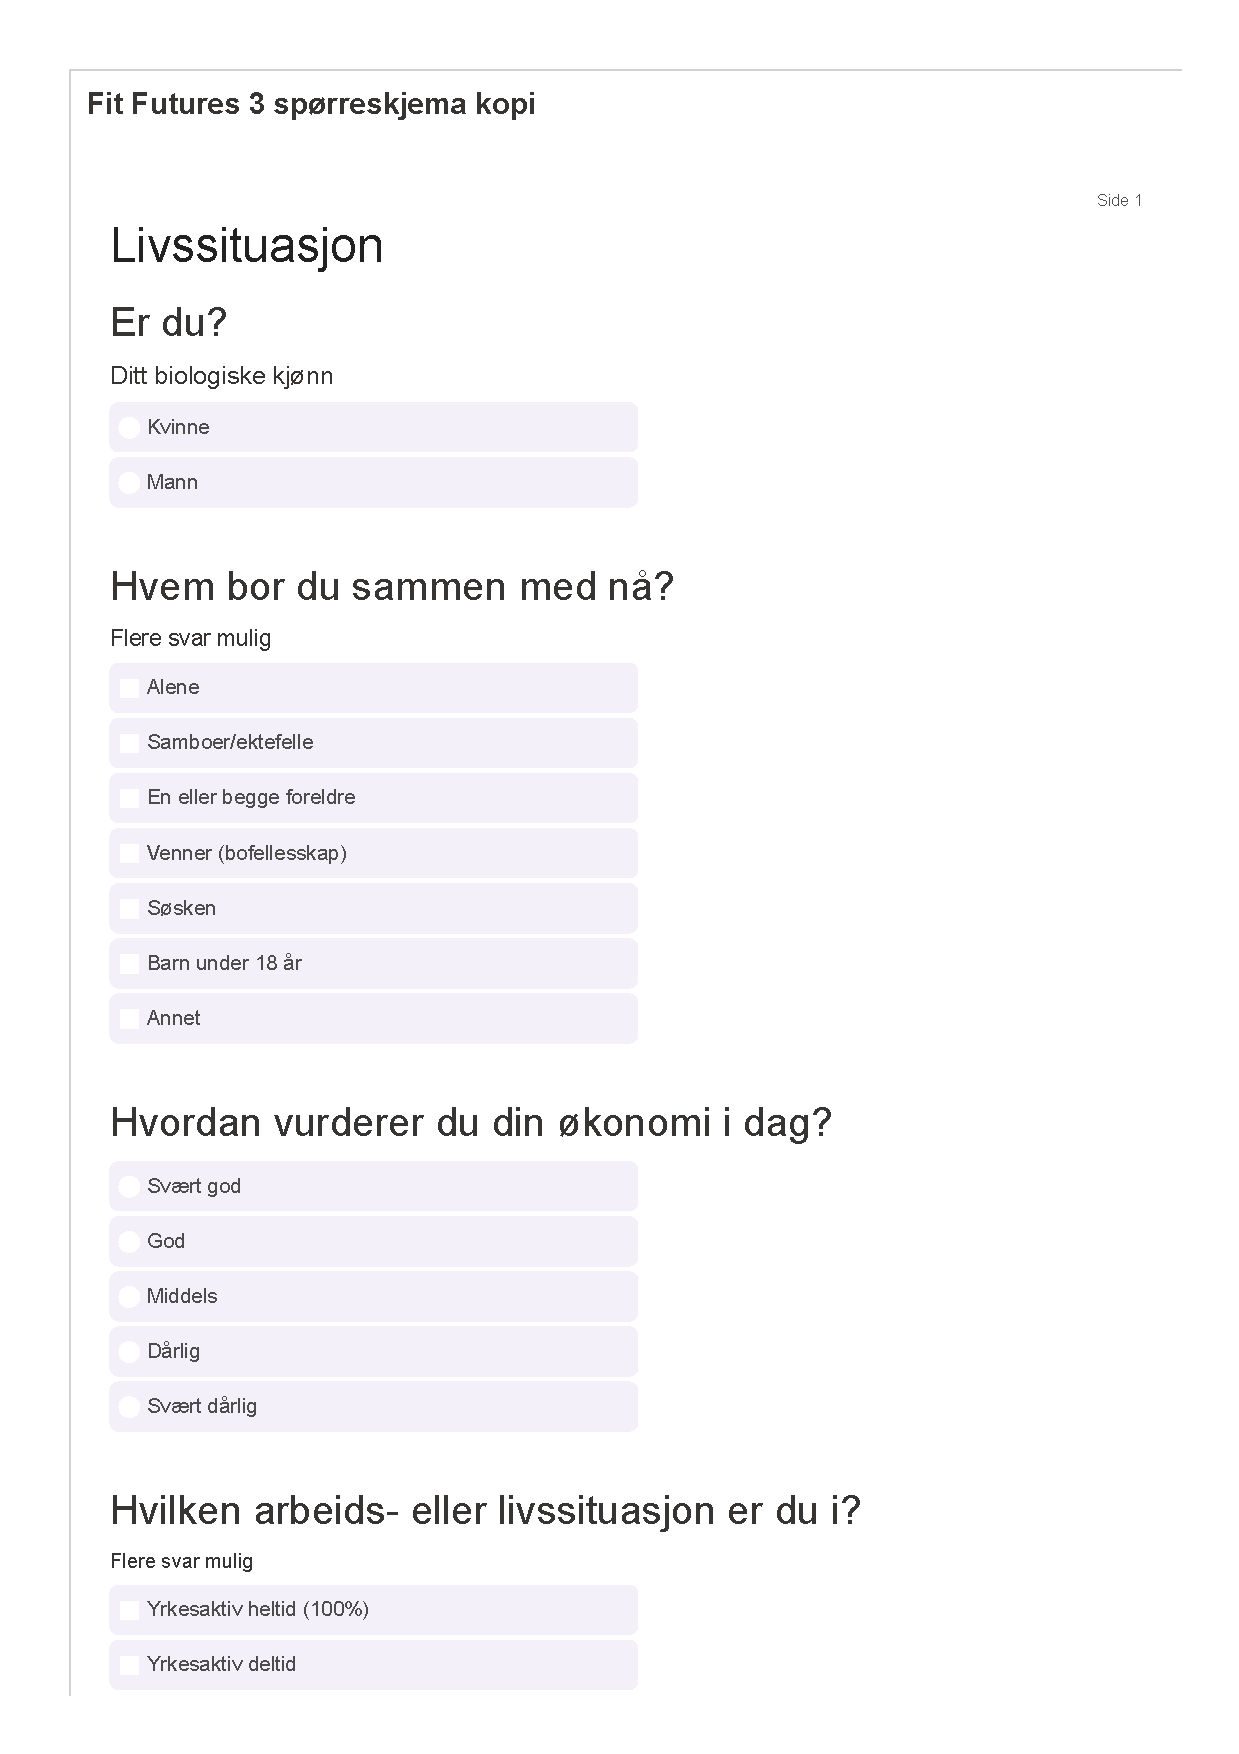
\includepdf[pages=1-32, nup=2x2, scale = 0.95, offset=30 -10]{Annex/FF3NOR_final_version.pdf}

%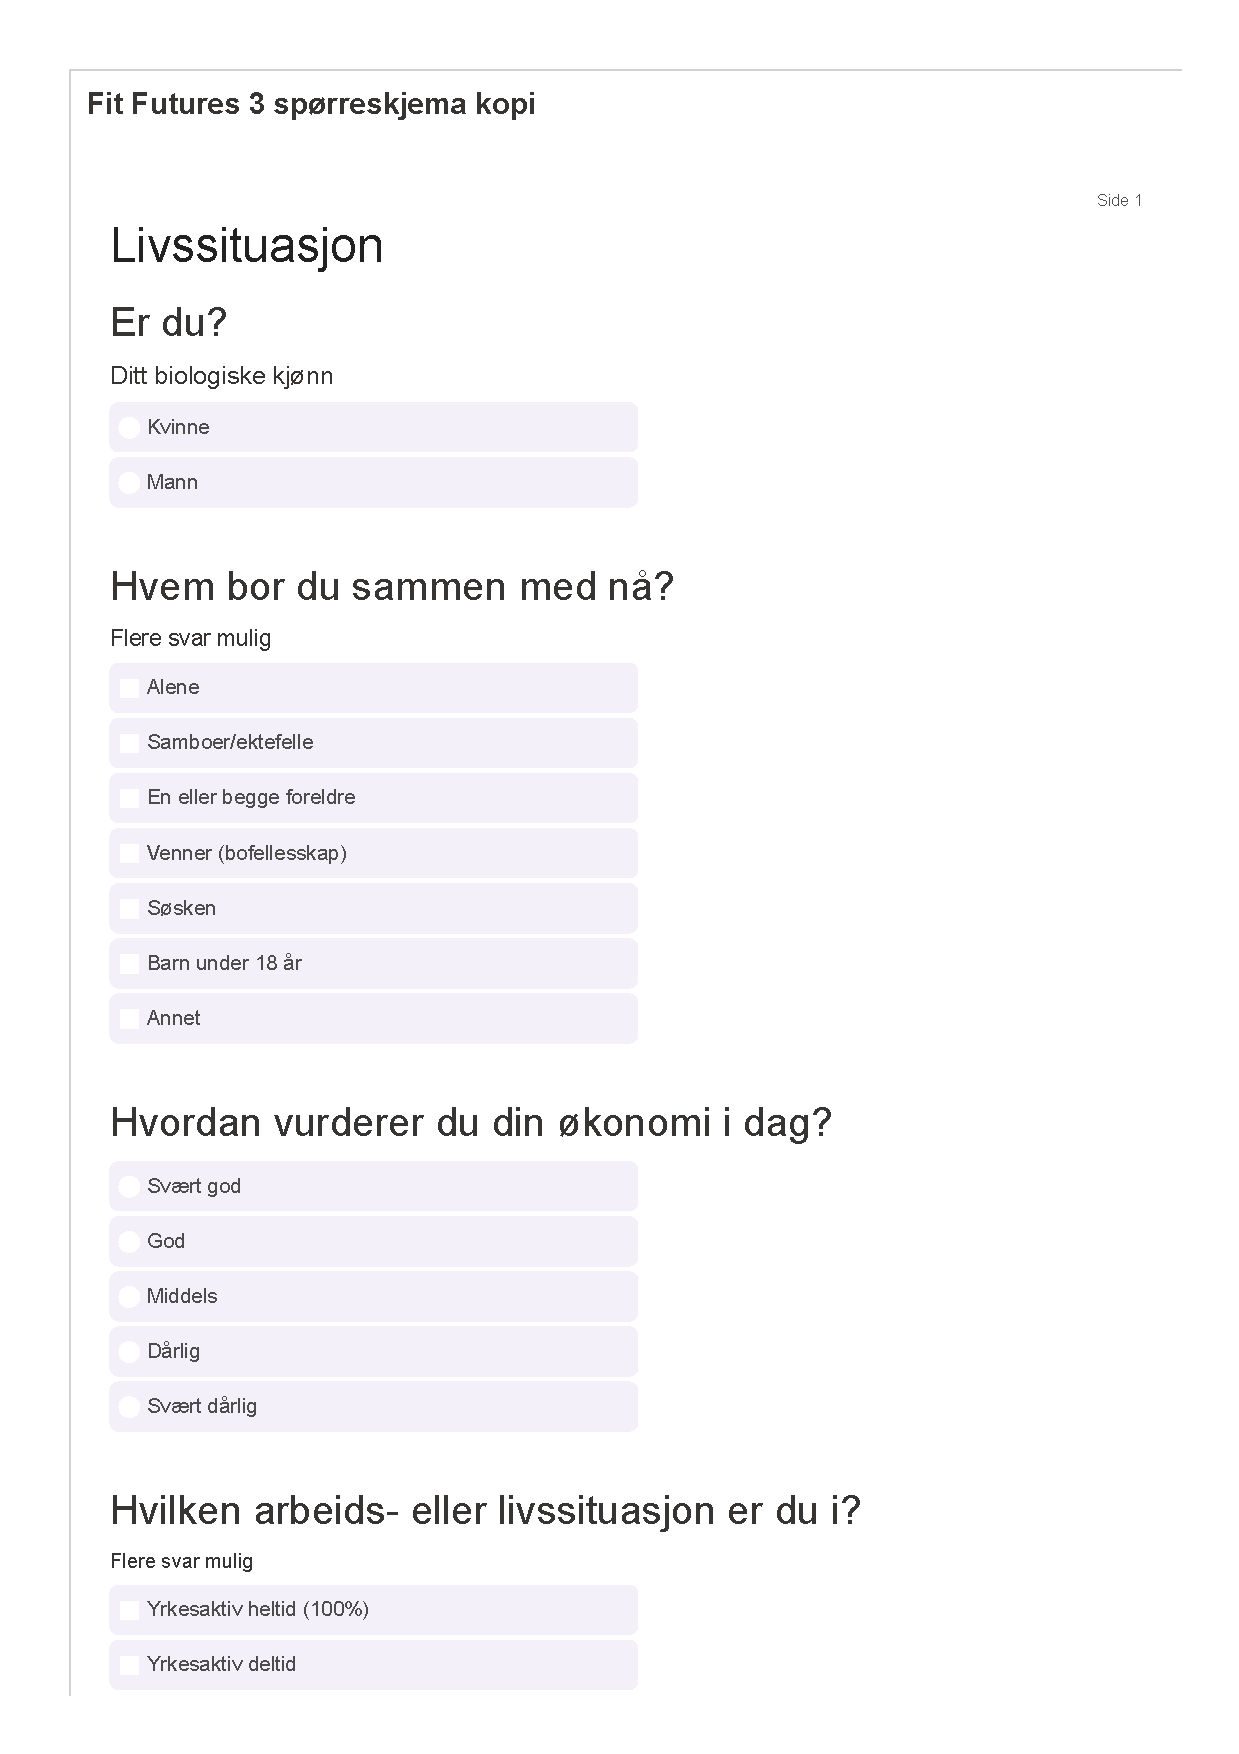
\includepdf[pages=1-32, nup=2x2, scale = 0.95, offset=0 190]{Annex/FF3NOR_final_version.pdf}

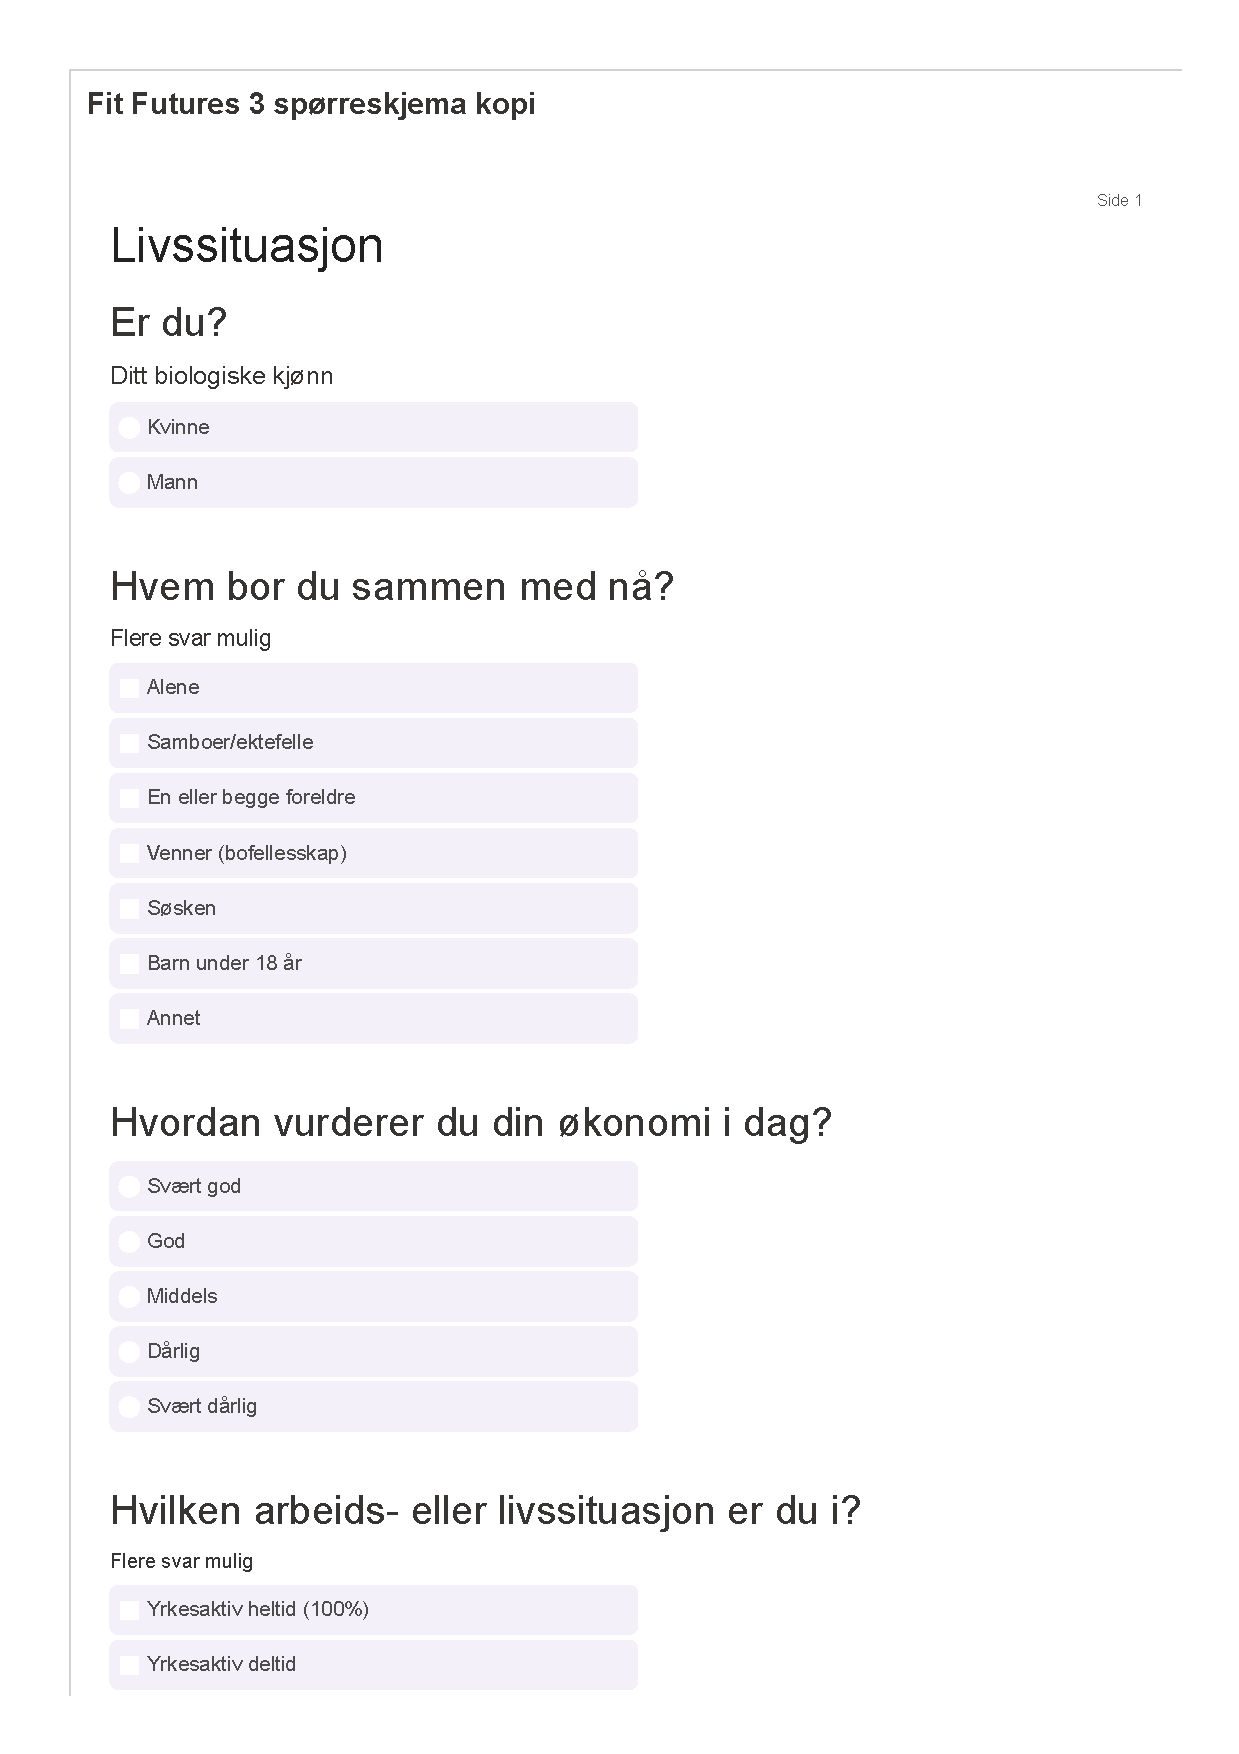
\includepdf[pages=1-32, width=\textwidth]{Annex/FF3NOR_final_version.pdf}       % Imports the contents from appendix.txt file 


\end{document}
